% So it begins ----------
\documentclass[a4paper,11pt,twoside]{report}
\usepackage[left=2.5cm,right=2.5cm,top=2.5cm,bottom=2.5cm]{geometry}

\usepackage[english]{babel}
\usepackage[utf8x]{inputenc} % for all the stylish Portuguese accents
\fontfamily{times}
\usepackage{titlesec}

\usepackage{setspace} % footnotes, figures and tables remain sigle-spaced
\parindent=0em
\parskip=12pt

%%%%%%%%%%%%%%%%%%%%%%%%
%%%%% PACKAGE FILE %%%%%
%%%%%%%%%%%%%%%%%%%%%%%%
% ADDED PACKAGES AND STRUCTURE OPTIONS ------------------------------

% %UHEAD.STY  If this is included after \documentstyle{report}, it adds
% an underlined heading style to the LaTeX report style.
% \pagestyle{uheadings} will put underlined headings at the top
% of each page. The right page headings are the Chapter titles and
% the left page titles are supplied by \def\lefthead{text}.

% Ted Shapin, Dec. 17, 1986

\makeatletter
\def\chapapp2{Chapter}

\def\appendix{\par
 \setcounter{chapter}{0}
 \setcounter{section}{0}
 \def\chapapp2{Appendix}
 \def\@chapapp{Appendix}
 \def\thechapter{\Alph{chapter}}}

\def\ps@uheadings{\let\@mkboth\markboth
% modifications
\def\@oddhead{\protect\underline{\protect\makebox[\textwidth][l]
		{\sl\rightmark\hfill\rm\thepage}}}
\def\@oddfoot{}
\def\@evenfoot{}
\def\@evenhead{\protect\underline{\protect\makebox[\textwidth][l]
		{\rm\thepage\hfill\sl\leftmark}}}
% end of modifications
\def\chaptermark##1{\markboth {\ifnum \c@secnumdepth >\m@ne
 \chapapp2\ \thechapter. \ \fi ##1}{}}%
\def\sectionmark##1{\markright {\ifnum \c@secnumdepth >\z@
  \thesection. \ \fi ##1}}}
\makeatother
% \setlength{\parskip}{12pt}        % a little space before a \par
\setlength{\parindent}{0pt}	      % don't indent first lines of paragraphs % identation?
% %%From: marcel@cs.caltech.edu (Marcel van der Goot)
%%Newsgroups: comp.text.tex
%%Subject: illegal modification of boxit.sty
%%Date: 28 Feb 92 01:10:02 GMT
%%Organization: California Institute of Technology (CS dept)
%%Nntp-Posting-Host: andromeda.cs.caltech.edu
%%
%%
%%Quite some time ago I posted a file boxit.sty; maybe it made it
%%to some archives, although I don't recall submitting it. It defines
%%	\begin{boxit}
%%	...
%%	\end{boxit}
%%to draw a box around `...', where the `...' can contain other
%%environments (e.g., a verbatim environment). Unfortunately, it had
%%a problem: it did not work if you used it in paragraph mode, i.e., it
%%only worked if there was an empty line in front of \begin{boxit}.
%%Luckily, that is easily corrected.
%%
%%HOWEVER, apparently someone noticed the problem, tried to correct it,
%%and then distributed this modified version. That would be fine with me,
%%except that:
%%1. There was no note in the file about this modification, it only has my
%%   name in it.
%%2. The modification is wrong: now it only works if there is *no* empty
%%   line in front of \begin{boxit}. In my opinion this bug is worse than
%%   the original one.
%%
%%In particular, the author of this modification tried to force an empty
%%line by inserting a `\\' in the definition of \Beginboxit. If you have
%%a version of boxit.sty with a `\\', please delete it. If you have my
%%old version of boxit.sty, please also delete it. Below is an improved
%%version.
%%
%%Thanks to Joe Armstrong for drawing my attention to the bug and to the
%%illegal version.
%%
%%                                          Marcel van der Goot
%% .---------------------------------------------------------------
%% | Blauw de viooltjes,                    marcel@cs.caltech.edu
%% |    Rood zijn de rozen;
%% | Een rijm kan gezet
%% |    Met plaksel en dozen.
%% |


% boxit.sty
% version: 27 Feb 1992
%
% Defines a boxit environment, which draws lines around its contents.
% Usage:
%   \begin{boxit}
%	... (text you want to be boxed, can contain other environments)
%   \end{boxit}
%
% The width of the box is the width of the contents.
% The boxit* environment behaves the same, except that the box will be
% at least as wide as a normal paragraph.
%
% The reason for writing it this way (rather than with the \boxit#1 macro
% from the TeXbook), is that now you can box verbatim text, as in
%   \begin{boxit}
%   \begin{verbatim}
%   this better come out in boxed verbatim mode ...
%   \end{verbatim}
%   \end{boxit}
%
%						Marcel van der Goot
%						marcel@cs.caltech.edu
%

\def\Beginboxit
   {\par
    \vbox\bgroup
	   \hrule
	   \hbox\bgroup
		  \vrule \kern1.2pt %
		  \vbox\bgroup\kern1.2pt
   }

\def\Endboxit{%
			      \kern1.2pt
		       \egroup
		  \kern1.2pt\vrule
		\egroup
	   \hrule
	 \egroup
   }	

\newenvironment{boxit}{\Beginboxit}{\Endboxit}
\newenvironment{boxit*}{\Beginboxit\hbox to\hsize{}}{\Endboxit}
   % to draw a box around the text - labels the page with the chapters
\makeatletter  %to avoid error messages generated by "\@". Makes Latex treat "@" like a letter


%%%%%%%%%% What do I need to fill %%%%%%%%%%
\def\university#1{\gdef\@university{#1}}
\def\faculty#1{\gdef\@faculty{#1}}
\def\dept#1{\gdef\@dept{#1}}
\def\title#1{\gdef\@title{#1}}
\def\masters#1{\gdef\@masters{#1}}
\def\supervisor#1{\gdef\@supervisor{#1}}
\def\supervisora#1{\gdef\@supervisora{#1}}
\def\submitdate#1{\gdef\@submitdate{#1}}
%%%%%%%%%%%%%%%%%%%%%%%%%%%%%%%%%%%%%%%%%%%%

%%%%%%%%%%%%%%%%%%%%%%
%%%%% TITLE PAGE %%%%%
%%%%%%%%%%%%%%%%%%%%%%
\def\maketitle{
    \begin{titlepage}
    \renewcommand{\baselinestretch}{1.5}
    \fontfamily{phv}\fontseries{mc}\selectfont
	\begin{center} \thispagestyle{empty}  
	\par{\LARGE \@university}\\
        \par{\LARGE \@faculty}\\
        \par{\LARGE \@dept}\\
	\vfill
	
	
\includegraphics[scale=0.25]{images/logo_fcul.pdf}
	
	\vfill
	\LARGE \textbf{Statistical approaches to measure heterogeneity in malaria transmission intensity:\\ An epidemiological study on the Tanzania populations}
	\vfill
	\par{\LARGE \@author}\\
	\vfill
	\large \textbf{Mestrado em Bioestatística} \\
	\vspace{1.2cm}
% 	\large Versão Provisória \\
	\vspace{0.8cm}
	\large Dissertação orientada por: \\
	%\vspace{1cm}
	\large Prof. Doutor Nuno Sepúlveda\\
	\large Prof.ª Doutora Marília Antunes\\
	\vfill
	\par{\large \@submitdate}
	\end{center}
\end{titlepage}
}

% \def\maketitle{
%   \begin{titlepage}
%   \thispagestyle{empty}
%     \begin{center}
        
%         \par{\LARGE \@university}\\
%         \par{\LARGE \@faculty}\\
%         \par{\LARGE \@dept}\\
        
%         \vspace{1.0cm}

% 		
\includegraphics[scale=0.25]{images/logo_fcul.pdf}\\
 
% 		\vspace{0.5cm}
        
%         \Huge
% 		\textbf{\@title}
        
%         \vspace{1.0cm}
        
%         \par{\LARGE \@author}\\
%         \vspace{1.0cm}
%         \Large
%         \textbf{\@masters}
        
%         \vspace{1.0cm}
%         \large
%         \textbf{(Versão provisória)}\\
%         Dissertação orientada por:\\\@supervisor\\\@supervisora

        
%         \vspace{1.0cm}
        
%         \par{\Large \@submitdate}
		
        

        
%     \end{center}
% \end{titlepage}
% }


\def\titlepage{
  \newpage
  \centering
  \linespread{1.15}
  \normalsize
  \vbox to \vsize\bgroup\vbox to 9in\bgroup
}

\def\endtitlepage{
  \par
  \kern 0pt
  \egroup
  \vss
  \egroup
  \cleardoublepage
}
%%%%%%%%%%%%%%%%%%
%%%%% RESUMO %%%%%
%%%%%%%%%%%%%%%%%%
\def\resumo{
  \begin{center}{
    \large\bf Resumo}
  \end{center}
  \small
%   \def\baselinestretch{1.15}
  \linespread{1.15}
  \normalsize
}
\def\endresumo{
  \par
}
%%%%%%%%%%%%%%%%%%%%
%%%%% ABSTRACT %%%%%
%%%%%%%%%%%%%%%%%%%%
\def\abstract{
  \begin{center}{
    \large\bf Abstract}
  \end{center}
  \small
%   \def\baselinestretch{1.15}
  \linespread{1.15}
  \normalsize
}
\def\endabstract{
  \par
}
%%%%%%%%%%%%%%%%%%%%%%%%%%%%
%%%%% ACKNOWLEDGEMENTS %%%%%
%%%%%%%%%%%%%%%%%%%%%%%%%%%%
\newenvironment{acknowledgements}{
  \cleardoublepage
  \begin{center}{
    \large \bf Acknowledgements}
  \end{center}
  \small
  \linespread{1.15}
  \normalsize
}{\cleardoublepage}
\def\endacknowledgements{
  \par
}
%%%%%%%%%%%%%%%%%%%%%%
%%%%% DEDICATION %%%%%
%%%%%%%%%%%%%%%%%%%%%%
\newenvironment{dedication}{
  \cleardoublepage
  \begin{center}{
    \large \bf Dedication}
  \end{center}
  \small
  \linespread{1.15}
  \normalsize
}{\cleardoublepage}
\def\enddedication{
  \par
}
%%%%%%%%%%%%%%%%%%%
%%%%% PREFACE %%%%%
%%%%%%%%%%%%%%%%%%%
\def\preface{
    \pagenumbering{roman}
    \pagestyle{plain}
    \doublespacing
}
%%%%%%%%%%%%%%%%
%%%%% BODY %%%%%
%%%%%%%%%%%%%%%%
\def\body{
    \cleardoublepage
    \makeatletter
    % \pagestyle{headings}
    \tableofcontents
    \pagestyle{plain}
    \cleardoublepage
    
    % \pagestyle{headings}
    \listoftables
    \pagestyle{plain}
    \cleardoublepage
    
    % \pagestyle{headings}
    \listoffigures
    \pagestyle{plain}
    \cleardoublepage
    
    % \pagestyle{headings}
    \pagenumbering{arabic}
    \linespread{1.15}
}
\makeatother  %to avoid error messages generated by "\@". Makes Latex treat "@" like a letter

% %%%%%%%%%%%%%%%%
% %%%%% BODY %%%%%
% %%%%%%%%%%%%%%%%
% \def\body{
%     %%% Contents %%%
%     % \cleardoublepage    
%     \pagestyle{uheadings}
%     \tableofcontents
%     \pagestyle{plain}
    
%     %%% Tables %%%
%     %\cleardoublepage
%     \pagestyle{uheadings}
%     \listoffigures
%     \pagestyle{plain}
%     %\cleardoublepage
    
%     %%% Figures %%%
%     \pagestyle{uheadings}
%     \listoftables
%     \pagestyle{plain}
%     %\cleardoublepage
    
%     %%% Chapters %%%
%     \pagestyle{uheadings}
% }

% \makeatother  %to avoid error messages generated by "\@". Makes Latex treat "@" like a letter % knit thesis structure


%%%%%%%%%%%%%%%%%%%%
%%%%% PACKAGES %%%%%
%%%%%%%%%%%%%%%%%%%%

\usepackage{adjustbox}
\usepackage{afterpage}
\usepackage{amsfonts}
\usepackage{amsmath} % for intense use of mathematical symbols
\usepackage{amssymb} % forarrows and such in equations
\usepackage{amsthm}
\usepackage{array}
\usepackage{auto-pst-pdf}
\usepackage[toc,page]{appendix}
\usepackage{bm} % bold symbols
\usepackage{booktabs}
\usepackage{breqn} % automatic line breaking in equations - useful
\usepackage[font=small, labelfont=bf]{caption}
\usepackage{color}
\usepackage{enumitem}
\usepackage{epsf}
\usepackage{epsfig}
\usepackage{epstopdf}
\usepackage{fancybox}
\usepackage{float} % figures and tables
\usepackage{geometry}
\usepackage{graphicx} % import graphics
\usepackage[hidelinks]{hyperref}  % for references and labels
\usepackage{latexsym} % some extra symbols
\usepackage{listings}
\usepackage{mathchars} % presentation of math characters
\usepackage{makecell}
\usepackage{multirow}
\usepackage[numbers,sort]{natbib} % citations
\usepackage{paralist}    % To enable customise enumerates
\usepackage{pst-plot}
\usepackage{pstricks}
\usepackage{pstricks-add}
\usepackage{rotating}
\usepackage{scrextend} % add lists
\usepackage{setspace} % set spacing between the lines
\usepackage{soul}
\usepackage{subcaption} % for subfigures
\usepackage{tabularx}
\usepackage{tikz}
\usepackage{tikzinput}
\usepackage[colorinlistoftodos, textwidth=60, textsize=small]{todonotes}
\usepackage[normalem]{ulem} % underline options
\usepackage{upgreek}
\usepackage{url} % allows linebreaks at certain characters or combinations of characters
\usepackage{verbatim} % comment environment
% \usepackage[svgnames]{xcolor}



%%%%%%%%%%%%%%%%%%%%%%%%%%%%%%%%
%%%%% EXTRAS FROM TEMPLATE %%%%%
%%%%%%%%%%%%%%%%%%%%%%%%%%%%%%%%

\let\origappendix\appendix % save the existing appendix command
\renewcommand\appendix{\clearpage\pagenumbering{roman}\origappendix}

\def\undertilde#1{\mathord{\vtop{\ialign{##\crcr $\hfil\displaystyle{#1}\hfil$\crcr\noalign{\kern1.5pt\nointerlineskip}
$\hfil\tilde{}\hfil$\crcr\noalign{\kern1.5pt}}}}}

\def\coop{\mbox{\large $\rhd\!\!\!\lhd$}}
\newcommand{\sync}[1]{\raisebox{-1.0ex}{$\;\stackrel{\coop}{\scriptscriptstyle
#1}\,$}}


%%%%%%%%%%%%%%%%%%%%%%%%
%%%%% NEW COMMANDS %%%%%
%%%%%%%%%%%%%%%%%%%%%%%%
\newcommand{\ipc}{{\sf ipc}}
\newcommand{\Prob}{\bbbp}
\newcommand{\Real}{\bbbr}
\newcommand{\real}{\Real}
\newcommand{\Int}{\bbbz}
\newcommand{\Nat}{\bbbn}
% syze of letters ------------------------------
\newcommand{\NN}{{\sf I\kern-0.14emN}}   % Natural numbers
\newcommand{\ZZ}{{\sf Z\kern-0.45emZ}}   % Integers
\newcommand{\QQQ}{{\sf C\kern-0.48emQ}}   % Rational numbers
\newcommand{\RR}{{\sf I\kern-0.14emR}}   % Real numbers
% mathematical letters ------------------------------
\newcommand{\KK}{{\cal K}}
\newcommand{\OO}{{\cal O}}
% bold letters ------------------------------
\newcommand{\AAA}{{\bf A}}
\newcommand{\HH}{{\bf H}}
\newcommand{\II}{{\bf I}}
\newcommand{\LL}{{\bf L}}
\newcommand{\PP}{{\bf P}}
\newcommand{\PPprime}{{\bf P'}}
\newcommand{\QQ}{{\bf Q}}
\newcommand{\UU}{{\bf U}}
\newcommand{\UUprime}{{\bf U'}}
\newcommand{\zzero}{{\bf 0}}
\newcommand{\ppi}{\mbox{\boldmath $\pi$}}
\newcommand{\aalph}{\mbox{\boldmath $\alpha$}}
\newcommand{\bb}{{\bf b}}
\newcommand{\ee}{{\bf e}}
\newcommand{\mmu}{\mbox{\boldmath $\mu$}}
\newcommand{\vv}{{\bf v}}
\newcommand{\xx}{{\bf x}}
\newcommand{\yy}{{\bf y}}
\newcommand{\zz}{{\bf z}}
\newcommand{\oomeg}{\mbox{\boldmath $\omega$}}
\newcommand{\res}{{\bf res}}
\newcommand{\cchi}{{\mbox{\raisebox{.4ex}{$\chi$}}}}
%\newcommand{\cchi}{{\cal X}}
%\newcommand{\cchi}{\mbox{\Large $\chi$}}
% Logical operators and symbols ------------------------------
\newcommand{\imply}{\Rightarrow}
\newcommand{\bimply}{\Leftrightarrow}
\newcommand{\union}{\cup}
\newcommand{\intersect}{\cap}
\newcommand{\boolor}{\vee}
\newcommand{\booland}{\wedge}
\newcommand{\boolimply}{\imply}
\newcommand{\boolbimply}{\bimply}
\newcommand{\boolnot}{\neg}
\newcommand{\boolsat}{\!\models}
\newcommand{\boolnsat}{\!\not\models}
\newcommand{\op}[1]{\mathrm{#1}}
\newcommand{\s}[1]{\ensuremath{\mathcal #1}}
% Properly styled differentiation and integration operators ------------------------------
\newcommand{\diff}[1]{\mathrm{\frac{d}{d\mathit{#1}}}}
\newcommand{\diffII}[1]{\mathrm{\frac{d^2}{d\mathit{#1}^2}}}
\newcommand{\intg}[4]{\int_{#3}^{#4} #1 \, \mathrm{d}#2}
\newcommand{\intgd}[4]{\int\!\!\!\!\int_{#4} #1 \, \mathrm{d}#2 \, \mathrm{d}#3}
% Large () brackets on different lines of an eqnarray environment ------------------------------
\newcommand{\Leftbrace}[1]{\left(\raisebox{0mm}[#1][#1]{}\right.}
\newcommand{\Rightbrace}[1]{\left.\raisebox{0mm}[#1][#1]{}\right)}
% Funky symbols for footnotes ------------------------------
\newcommand{\symbolfootnote}{\renewcommand{\thefootnote}{\fnsymbol{footnote}}}
% now add \symbolfootnote to the beginning of the document...
\newcommand{\normallinespacing}{\renewcommand{\baselinestretch}{1.15} \normalsize}
\newcommand{\mediumlinespacing}{\renewcommand{\baselinestretch}{1.2} \normalsize}
\newcommand{\narrowlinespacing}{\renewcommand{\baselinestretch}{1.0} \normalsize}
\newcommand{\bump}{\noalign{\vspace*{\doublerulesep}}}
\newcommand{\cell}{\multicolumn{1}{}{}}
\newcommand{\spann}{\mbox{span}}
\newcommand{\diagg}{\mbox{diag}}
\newcommand{\modd}{\mbox{mod}}
\newcommand{\minn}{\mbox{min}}
\newcommand{\andd}{\mbox{and}}
\newcommand{\forr}{\mbox{for}}
\newcommand{\EE}{\mbox{E}}
\newcommand{\deff}{\stackrel{\mathrm{def}}{=}}
\newcommand{\syncc}{~\stackrel{\textstyle \rhd\kern-0.57em\lhd}{\scriptstyle L}~}


\newtheorem{definition}{Definition}[chapter]
\newtheorem{theorem}{Theorem}[chapter] % this document has all the packages, newcomands lines and the rest of the Latex macropages (.sty)

\makeatletter
    \def\thebibliography#1{\chapter*{References\@mkboth
      {REFERENCES}{REFERENCES}}\list
      {[\arabic{enumi}]}{\settowidth\labelwidth{[#1]}\leftmargin\labelwidth
	\advance\leftmargin\labelsep
	\usecounter{enumi}}
	\def\newblock{\hskip .11em plus .33em minus .07em}
	\sloppy\clubpenalty4000\widowpenalty4000
	\sfcode`\.=1000\relax}
    \makeatother

\begin{document}

%%%%%%%%%%%%%%%%%%%%%%
%%%%% TITLE PAGE %%%%%
%%%%%%%%%%%%%%%%%%%%%%
% What do I need to fill -----
\title{\LARGE {\bf Statistical approaches to measure heterogeneity in malaria transmission intensity:\\ An epidemiological study on the Tanzania populations}\\
\vspace*{6mm}
}
\university{Universidade de Lisboa}
\faculty{Faculdade de Ciências}
\dept{Departamento de Estatística e Investigação Operacional}
\author{João Torrado Malato}
\masters{Mestrado em Bioestatística}
\supervisor{Prof. Doutor Nuno Sepúlveda}
\supervisora{Prof.ª Doutora Marília Antunes}
\submitdate{2018}
%%%%%%%%%%%%%%%%%%%%%%
\maketitle % title page

%%%%%%%%%%%%%%%%%%%
%%%%% PREFACE %%%%%
%%%%%%%%%%%%%%%%%%%

\preface % all this needs to have ROMAN NUMERATION
\clearpage

\narrowlinespacing

\vspace*{4mm}

%``Não se pode só analisar os dados, há que saber criar e contar a sua história.''\\

\noindent
``A análise dos dados por si só nunca nos serve de muito. Há que saber contar a sua história.''

\emph{--- Nuno Sepúlveda}

\noindent
\\
\\

``Ainda que não pareça, o ótimo é inimigo do bom. Respira fundo, sem medo!''

\emph{--- Marília Antunes}

\normallinespacing


%\cleardoublepage

\addcontentsline{toc}{chapter}{Acknowledgements}

\begin{acknowledgements}

I would like to thank everyone who directly and indirectly contributed to the realisation of this Biostatistics MSc thesis.
First of all, my supervisor, Nuno for providing me with the opportunity to work, develop, and prepare my project and dissertation in the field of malaria epidemiology and modelling of infectious diseases.
Moreover, thank you for all the advises, ideas, and continuous constructive criticism (as well as all the Wednesdays afternoon football games) that have already proven to be valuable teachings to take into the future.
I also want to thank my co-supervisor, Marília, for all the Skype pep talks and helpful suggestions during the later stages of the dissertation that kept me motivated and helped to further improve the thesis.
I am grateful for the opportunity to prepare this project at two institutions.
First, the London School of Hygiene and Tropical Medicine (LSHTM). Particularly acknowledging all members from the Chris Drakeley's group, whom during my time abroad made me feel welcome to work in a specialised and fully dedicated research group. Cheers to you!
And second, the Faculty of Sciences at the University of Lisbon (FCUL), that alongside with the Erasmus+ programme allowed me to travel abroad and learn new research fields, amazing organisations, and terrific people.

E agora em português.
Quero agradecer a todos aqueles que me apoiaram no projecto e escrita da tese.
Um obrigado a toda a minha família, principalmente aos meus pais e irmãos por me ajudarem com as viagens para a frente e para trás ao longo deste ano, e por constantemente zelarem pelo meu bem estar.
Um beijo especialmente carinhoso à minha Mãe por todos os telefonemas, cartas e mimos que disponibilizou.
Logo que concluir esta tese, será a primeira a quem vou ligar.
Aos meus colegas de mestrado um muito obrigado.
Especialmente ao Bruno, Heloísa, e Sofia, por me terem ajudado a entrar ná área da estatística ao longo dos dois anos do mestrado; e ao Constantino, por todos os debates, explicações e demonstrações, e por não esperar menos do que o melhor de mim, ao fazer de criticar esta tese um passatempo.
Obrigado ainda à minha família alargada e aos mais variados amigos, que se preocuparam e me fizeram companhia ao longo do ano.

Mais que todos, mil obrigados à Dida, por tudo.
\\
Obrigado Formiguita.

\begin{flushright}
João Malato,\\
Lisboa, Outubro de 2018.\\
\end{flushright}

\end{acknowledgements}

\newpage
\addcontentsline{toc}{chapter}{Resumo}

\begin{resumo}

% \begin{itemize}
% % What's the problem?
% 	\item Qual é o problema?
% % Why is it interesting?
% 	\item Porque é que ele é interessante?
% % What's the solution?
% 	\item Qual é a solução?
% % What follows from the solution?
% 	\item O que resulta (implicações) da solução?
% \end{itemize}
A malária (paludismo) é uma doença infecciosa, reconhecida, nas últimas décadas, como sendo um dos maiores desafios para a saúde pública.
A malária é endémica em grande parte da Africa Subsaariana, Sudeste asiático e América Latina, estimando-se cerca de 216 milhões de novos casos de infeção e 445 000 mortes, só em 2016.
Os estudos produzidos nos últimos anos têm permitido abordagens efetivas para o controlo e para uma eliminação mais eficiente dos seus transmissores (os mosquitos do género \textit{Anopheles}), bem como o desenvolvimento de tratamentos diretos na redução do parasita \textit{Plamodium falciparum}, a espécie mais incidente nos países da Africa Subsaariana.
Com estes avanços, a incidência de malária tem gradualmente vindo a ser reduzida, havendo cada vez mais áreas a transitar para estados de pré-eliminação e eliminação.
Devido a estes desenvolvimentos, surgem novos desafios para a estimação da incidência dos locais e da intensidade de transmissão.
As regiões onde a intensidade de transmissão é mantida baixa produzem infeções assintomáticas, tornando os indivíduos neste estado transmissores “invisíveis” de malária, uma vez que os métodos mais comuns para medir os níveis de malária baseiam-se na deteção objetiva de casos de infeção.
Como alternativa a estas medidas, surge a serologia, aplicada em análises sero-epidemiológicas.
Este método põe de lado a análise de indivíduos infetados/não infetados, passando a lidar com a exposição/não exposição dos indivíduos ao parasita \textit{P. falciparum} e o desenvolvimento de anticorpos pelo sistema imunitário.
A serologia mede e identifica a presença de anticorpos específicos para antigénios do parasita, podendo definir um gradiente para a intensidade de transmissão de uma dada população analisada, mesmo em locais de baixa incidência.

Esta tese teve como objetivo descrever e estimar a intensidade de transmissão do parasita \textit{P. falciparum} de uma amostra estratificada de 5058 indivíduos distribuídos em 21 vilas ao longo do Nordeste da Tanzânia.
Estes dados foram originalmente recolhidos e aplicados num estudo de referência para a área de sero-epidemiologia, tendo como intuito estimar a intensidade de transmissão associada às variáveis altitude e precipitação.

Numa primeira abordagem, os principais fatores de risco associados à prevalência de infeção e heterogeneidade nos vários locais foram identificados.
Através da construção e seleção do melhor modelo linear generalizado (generalised linear model, GLM), a influência destes determinantes de transmissão foi estudada.
Nesta análise, determinantes representativos da altitude, agregado de vilas, grupo étnico, ou grupo etário, demonstraram ter uma influência significativa quando adicionados no modelo, tendo um efeito direto na probabilidade de infeção.
O GLM também caracterizou os três determinantes de exposição usados, relativos aos três antigénios estudados ao longo do projeto: merozoite surface protein 1 (MSP1), merozoite surface protein 2 (MSP2) e apical merozoite antigen 1 (AMA1).
A presença destes determinantes no modelo demonstrou a sua utilidade como bons indicadores de infeções de malária, aumentando muito a probabilidade de infeção de indivíduos sempre que estavam presentes.

Tendo identificado os anticorpos para os antigénios como uma alternativa ao estado de infeção das populações, a segunda parte da tese aplicou diferentes propostas sero-epidemiológicas para estudar a intensidade de transmissão das diferentes vilas estudadas.
Para tal, diferentes modelos catalíticos reversíveis (reverse catalytic models, RCMs) foram propostos.
Estes modelos baseiam-se na ideia de que indivíduos transitam entre dois estados serológicos (seronegativo e seropositivo), transitando de um para outro a diferentes taxas de transição, a taxa de seroconversão (seroconversion rate, SCR) e a taxa de serorreversão (seroreversion rate, SRR).
A SCR representa a taxa média anual a que indivíduos de uma determinada idade (em anos) passam de seronegativos para seropositivos, após uma infeção.
Já a SRR representa a taxa média anual a que indivíduos seropositivos regressam a um estado seronegativo devido ao decaimento gradual dos anticorpos.

Quatro RCMs foram aplicados aos dados serológicos.
Um primeiro modelo M$_{0}$ assumiu as taxas SCR e SRR como constantes ao longo de todas as idades.
Dois modelos consideraram SRR dependente da idade, M$_{1,1}$ e M$_{1,2}$.
Os dois modelos assumiram a SCR de cada vila como constante ao longo da sequência de idades e a ocorrência de uma redução de SRR dada uma idade estimada.
O modelo M$_{1,2}$ representava uma versão mais restrita, considerando que após a idade de redução, a SRR era igual a zero.
Por fim, o RCM M$_{2}$ proposto considerava a ocorrência de algum efeito externo (e.g.: campanhas de intervenção e prevenção de malária nos locais estudados) que tenha ocorrido nas últimas décadas, influenciando a intensidade de transmissão.
Este modelo assumiu a SRR estimada como constante ao longo dos anos, com uma variação na SCR, acontecendo um número estimado de anos antes da recolha das amostras.

Os resultados deste estudo mostraram que qualquer um dos modelos tem o potencial de descrever a intensidade de transmissão, bem como a seroprevalência das várias vilas estudadas.
A análise dos resultados dos diferentes modelos mostrou que as propostas tidas como mais próximas da realidade (modelos M$_{1,2}$ e M$_{0}$ ) foram rejeitadas, na sua maioria, quando comparadas com o modelo de taxas constantes, M$_{0}$ (testes de razão de verosimilhanças, valores-p $>0.05$).
O modelo M$_{1,2}$, com SRR dependente da idade, foi apenas significativo numa minoria de vilas a altitudes intermédias (altitudes entre os 600 e os 1200 metros).
A não rejeição da hipótese nula, aquando da comparação com o modelo M$_{2}$, demonstrou poucos episódios significativos onde a alteração de intensidade de transmissão foi observável.
Este modelo foi apenas significativo em vilas com maiores taxas de transmissão estimadas, a altitudes baixas e intermédias.

Os RCM ainda que sejam modelos específicos para populações infinitas produziram estimativas paramétricas aceitáveis.
Uma análise de correlação entre M$_{0}$ e M$_{1,2}$ demonstrou que o modelo estatisticamente preferido, tendencialmente subestimou as estimativas de SCR.
Esta taxa, um \textit{proxy} da intensidade de transmissão, é geralmente a medida de interesse nas análises sero-epidemiológicas.
Situações de baixa intensidade de transmissão, que requerem uma maior precisão das estimativas, devem ter em conta estes resultados dados por M$_{0}$.
O melhoramento dos modelos M$_{1,1}$ e M$_{1,2}$ poderá trazer novos resultados sobre a importância da SRR na estimação mais precisa das intensidades de transmissão.
Já o modelo M$_{2}$ continuará a servir como uma ferramenta para controlo e evolução do estado serológico das populações intervencionadas.

Os dois modelos que consideram o efeito ao longo do tempo do sistema imunitário em regiões de malária endémica, M$_{1,1}$ e M$_{1,2}$, foram desenvolvidos paralelamente a esta tese, tendo sido propostos num artigo científico presentemente em avaliação.

\textbf{Palavras-chave:} malária, intensidade de transmissão, heterogeneidade de transmissão, epidemiologia, serologia, seroprevalência, taxa de seroconversão, taxa de seroreversão.

\end{resumo}

\newpage

\addcontentsline{toc}{chapter}{Abstract}

\begin{abstract}

% To this day, malaria continues to be a worldwide cause of death and disease.
% With the recent decades bringing insightful research studies, campaigns for control and elimination became more efficient, gradually reducing the \textit{Plasmodium falciparum} parasitic malaria across sub-Saharan African countries.
% Such actions have resulted in regions of pre-elimination going into elimination stages, where detectable symptomatic infections are almost vestigial.
% These scenarios may impose a new challenge, as the more usual methodologies do not consider apparent invisible individuals when estimating malaria transmission intensity and its prevalence of infection.
% As a proposed alternative to this question, sero-epidemiology can be used to more accurately perform such inferences.

% The objective of this project is then to estimate and characterise the \textit{P. falciparum} transmission intensity from a sample of 5058 individuals structured by age groups, from across 21 villages in the Northeast Tanzania, with different prevalence levels.
% First, the principal transmission determinants influencing the infection heterogeneity were identified.
% Using the generalised linear models (GLMs) the study revealed the importance of some demographical risk factors when assessing the presence/absence of infection.
% Determinants such as the age group of the individuals, the altitude of a village -- a known proxy of transmission intensity --, or the transect in which the villages are encompassed, were some of the more impactful demographical transmission determinants assessed.
% The detected antimalarial antibodies for the specific antigens MSP1, MSP2, and AMA1, used throughout this thesis, were also included in the GLMs and showed the importance these exposure determinants have as reasonable indicators of malaria infection.
% The inference then led to the use of different reverse catalytic models (RCMs), applied solely to the serological data sets of the three antigens collected. 

% The RCMs assume that individuals transit between two possible serological states (seronegative and seropositive) at distinct rates: seroconversion rate (SCR) and seroreversion rate (SRR).
% The SCR is the annual average rate by which the individuals of a certain age change from seronegative to seropositive, upon malaria infection.
% And the SRR is the annual average rate by which seropositive individuals of a certain age return to the seronegative state due to antibody decay.
% Focusing on different biological and epidemiological proposals -- that might present an effect on the annual transitional rates between seronegative and seropositive individuals due to parasite exposure -- four RCMs were tested.
% Model M$_0$ assumed the seroconversion rate (SCR) and the seroreversion rate (SRR) as constant transition values across all ages.
% Models M$_{1,1}$ and M$_{1,2}$ were built to adjust for the biological effect of gradually developing immunity over time, in a scenario of endemic malaria transmission.
% Both models assumed SCR as constant over time, with SRR being reduced to a second rate given an estimated cutoff.
% Model M$_{1,2}$, a more restrictive version, assumed that the reduced SRR would be equal to zero, with no seropositive individuals transiting into a seronegative state after the age cutoff.
% Finally, model M$_{2}$ proposed the epidemiological effect that some event (e.g.: possible campaigns or interventions to prevent malaria) might have had on transmission intensity.
% This model assumed SRR as constant rate across all ages, with a change in SCR happening under an estimated cutoff sometime before the sampling. 

% The results showed that, depending on the antigen, the models could be used to describe the transmission intensity and seroprevalence of the assessed villages.
% However, the traditional RCM M$_{0}$ (transitional rates constant over time) was more often preferred when compared to the age-dependent M$_{1,2}$ (likelihood ratio test, p-values $>0.05$).
% The age-dependent SRR model was only significant when applied to some villages at intermediate altitudes (600 meters to 1200 meters high).
% The traditional model was also chosen in favour of the model admitting a past change in transmission intensity, M$_{2}$, with the epidemiological model only identifying a change in few villages placed at low and intermediate altitudes.
% Despite the limited information to estimate some of the models' parameters, further analyses demonstrated that the statistically and overall more parsimonious model M$_0$ produced underestimations in its transitional rates, when compared to the more realistic model M$_{1,2}$.
% This underestimation could have a negative impact when estimating malaria transmission intensity in low transmission scenarios.
% Sided with the newly formulated strategies to advance sites in stages of malaria elimination and pre-elimination into eradication, serology serves as tool to more efficaciously measure transmission intensity.
% The improvement and application of the RCMs M$_{1,1}$ and M$_{1,2}$ could bring more information to the importance of a more precise estimation of the SRR.
To this day, malaria continues to be a worldwide cause of death and disease.
With the recent decades bringing insightful research studies, campaigns for control and elimination became more efficient, gradually reducing the \textit{Plasmodium falciparum} parasitic malaria across sub-Saharan African countries.
Such actions have resulted in regions of pre-elimination going into elimination stages, where detectable symptomatic infections are almost vestigial.
These scenarios may impose a new challenge, as the more usual methodologies do not consider apparent invisible individuals when estimating malaria transmission intensity and prevalence of infection.
As a proposed alternative to this question, sero-epidemiology can be used to more accurately perform such inferences.

The objective of this thesis is then to estimate and characterise the \textit{P. falciparum} transmission intensity from a sample of 5058 individuals structured by age groups, from across 21 villages in the Northeast Tanzania, with different prevalence levels.
First, the principal transmission determinants influencing the infection heterogeneity were identified.
Using the generalised linear models (GLMs) the study revealed the importance of some demographical risk factors when assessing the presence/absence of infection.
Determinants such as the age group of the individuals, the altitude of a village -- a known proxy of transmission intensity --, or the transect in which the villages were encompassed, were some of the more impactful demographical transmission determinants assessed.
The detected antimalarial antibodies for the specific antigens MSP1, MSP2, and AMA1, used throughout this thesis, were also included in the GLMs and showed the importance these exposure determinants have as reasonable indicators of malaria infection.
The inference then led to the use of different reverse catalytic models (RCMs), applied solely to the serological data sets of the three antigens collected.

The RCMs assume that individuals transit between two possible serological states (seronegative and seropositive) at distinct rates: seroconversion rate (SCR) and seroreversion rate (SRR).
The SCR is the annual average rate by which the individuals of a certain age change from seronegative to seropositive, upon malaria infection.
And the SRR is the annual average rate by which seropositive individuals of a certain age return to the seronegative state due to antibody decay.
Focusing on different biological and epidemiological proposals -- that might present an effect on the annual transitional rates between seronegative and seropositive individuals due to parasite exposure -- four RCMs were tested.
Model M$_{0}$ assumed the seroconversion rate (SCR) and the seroreversion rate (SRR) as constant transition values across all ages.
Models M$_{1,1}$ and M$_{1,2}$ were built to adjust for the biological effect of gradually developing immunity over time, in a scenario of endemic malaria transmission.
Both models assumed SCR as constant over time, with SRR being reduced to a second rate given an estimated cutoff.
Model M$_{1,2}$, a more restrictive version, assumed that the reduced SRR would be equal to zero, with no seropositive individuals transiting into a seronegative state after the age cutoff.
Finally, model M$_{2}$ proposed the epidemiological effect that some event (e.g.: possible campaigns or interventions to prevent malaria) might have had on transmission intensity. 
This model assumed SRR as constant rate across all ages, with a change in SCR happening under an estimated cutoff sometime before the sampling.

The results showed that, depending on the antigen, the models could be used to describe the transmission intensity and seroprevalence of the assessed villages.
However, the traditional RCM M$_{0}$ (transitional rates constant over time) was more often preferred when compared to the age-dependent M$_{1,2}$ (likelihood ratio test, p-values $>0.05$). The age-dependent SRR model was only significant when applied to some villages at intermediate altitudes (600 meters to 1200 meters high). The traditional model was also chosen in favour of the model admitting a past change in transmission intensity, M$_{2}$, with the epidemiological model only identifying a change in few villages placed at low and intermediate altitudes.
Despite the limited information to estimate some of the models' parameters, further analyses demonstrated that the statistically and overall more parsimonious model M$_{0}$ produced underestimations in its transitional rates, when compared to the more realistic model M$_{1,2}$.
This underestimation could have a negative impact when estimating malaria transmission intensity in low transmission scenarios.
Sided with the newly formulated strategies to advance sites in stages of malaria elimination and pre-elimination into eradication, serology serves as tool to more efficaciously measure transmission intensity.
The improvement and application of the RCMs M$_{1,1}$ and M$_{1,2}$ could bring more information to the importance of a more precise estimation of the SRR.

\textbf{Keywords:} malaria, transmission intensity, transmission heterogeneity, epidemiology, serological data, seroprevalence, seroconversion rate, seroreversion rate.


\end{abstract}

%\cleardoublepage

\begin{dedication}
  Dedication here.
\end{dedication}



%%%%%%%%%%%%%%%%
%%%%% BODY %%%%%
%%%%%%%%%%%%%%%%
\body
%%%%%%%%%%%%%%%%%%%%%%%%%%
%%%%%   INTRODUCTION %%%%%
%%%%%%%%%%%%%%%%%%%%%%%%%%
\chapter{Introduction}
\label{ch:1.0}

% % \usepackage{multirow}
% % \usepackage{booktabs}
% \begin{table}
% \centering
% \begin{tabular}{llccc} 
% \toprule
% \multicolumn{1}{c}{\multirow{2}{*}{Transect}} & \multicolumn{1}{c}{\multirow{2}{*}{Village}} & \multicolumn{3}{c}{Selected RCM}    \\ 
% \cmidrule{3-5}
% \multicolumn{1}{c}{}                          & \multicolumn{1}{c}{}                         & MSP1       & MSP2     & AMA1        \\ 
% \midrule
% Rombo                                         & Mokala                                       & M$_{0}$    & M$_{0}$  & M$_{0}$     \\
%                                               & Machame Aleni                                & M$_{0}$    & M$_{0}$  & M$_{1,2}$   \\
%                                               & Ikuini                                       & M$_{0}$    & M$_{0}$  & M$_{0}$     \\
%                                               & Kileo                                        & M$_{0}$    & M$_{0}$  & M$_{0}$     \\ 
% \cmidrule{2-5}
% N. Pare                                       & Kilomeni                                     & M$_{0}$    & M$_{0}$  & M$_{0}$     \\
%                                               & Lambo                                        & M$_{0}$    & M$_{0}$  & M$_{0}$     \\
%                                               & Ngulu                                        & M$_{0}$    & M$_{0}$  & M$_{0}$     \\
%                                               & Kambi ya Simba                               & M$_{0}$    & M$_{0}$  & M$_{0}$     \\ 
% \cmidrule{2-5}
% S. Pare                                       & Bwambo                                       & M$_{0}$    & M$_{2}$  & M$_{0}$     \\
%                                               & Mpinji                                       & M$_{1,2}$  & M$_{2}$  & M$_{0}$     \\
%                                               & Goha                                         & M$_{0}$    & M$_{0}$  & M$_{1,2}$   \\
%                                               & Kadando                                      & M$_{0}$    & M$_{0}$  & M$_{0}$     \\ 
% \cmidrule{2-5}
% W. Usamb. 1                                   & Emmao                                        & M$_{0}$    & M$_{0}$  & M$_{0}$     \\
%                                               & Handei                                       & M$_{0}$    & M$_{0}$  & M$_{0}$     \\
%                                               & Tewe                                         & M$_{0}$    & M$_{0}$  & M$_{0}$     \\
%                                               & Mn'galo                                      & M$_{0}$    & M$_{0}$  & M$_{0}$     \\ 
% \cmidrule{2-5}
% W. Usamb. 2                                   & Kwadoe                                       & M$_{2}$    & M$_{0}$  & M$_{0}$     \\
%                                               & Funta                                        & M$_{0}$    & M$_{2}$  & M$_{0}$     \\
%                                               & Tamota                                       & M$_{2}$    & M$_{2}$  & M$_{0}$     \\
%                                               & Mgila                                        & M$_{2}$    & M$_{0}$  & M$_{0}$     \\ 
% \cmidrule{2-5}
% W. Usamb. 3                                   & Mgome                                        & M$_{2}$    & M$_{0}$  & M$_{0}$     \\
% \bottomrule
% \end{tabular}
% \end{table}

%This chapter describes the fundamental concepts used throughout the thesis.
%Section \ref{seq:malaria.intro} introduces the theme of malaria as a global disease.
%A brief description of malaria and its burden in human populations, focusing the current panorama for malaria epidemiology in tropical and subtropical countries.
%Epidemiological tools used to estimate malaria transmission intensity are described in Section \ref{seq:estimating}, distinguishing between the currently most used approaches and explaining why serology could be an alternative.
%An example of an important serological study is shown in Section \ref{seq:example}, where sero-epidemiology was used beyond the classical tools in order to estimate malaria transmission intensity with positive results.
%Section \ref{seq:objectives} describes the outline structure of the present thesis, explaining the objectives that led to its development at the London School of Hygiene and Tropical Medicine.
%A brief description of its development alongside the human populations and a description of current panorama for malaria epidemiology in tropical and subtropical countries are made in Section \ref{seq:malaria.intro}.
%is then introduced, where recent (and consecutive) interventions in these sites continue to decrease the risk of contracting malaria.
%An example of application using sero-epidemiological methods is given in Section \ref{seq:example} with the present challenges briefly described in Section \ref{seq:challenges}.
%Section \ref{seq:objectives} makes a short description of the outline of the present thesis, as well as the fundamental objectives that led this project to gain shape.
%adjusts as the `classical' tools developed to measure situations of high malaria transmission intensity may present limitations when it comes to measure low endemic malaria transmission intensity.
%Malaria is a severe public health problem and remains the leading cause of death in developing countries.

Malaria is a parasitic disease described since ancient times, and until this day it continues to be a major health problem.
% With approximately 400 million people world-wide currently infected and estimates
Despite continuous worldwide efforts and investments, malaria is still the principal cause of death and disease caused by a parasite \cite{vitoria2009global}, with estimates for 216 million new infection cases and 445 000 deaths globally in 2016 \cite{who2017world}.
%continuously being a leading cause of death and disease across many tropical and subtropical countries, going as far as exerting selective pressures, such is the example of the sickle cell trait as a protective adaptation \cite{}.
The term malaria originates from the 18th century italian expression \textit{mala aria}, meaning `bad air', referring the foul air evaporating from stagnant waters of marshes that used to be thought as the origin of the disease \cite{warrell2002essential}.
The real causative agent of malaria was only discovered in 1897, after Ronald Ross identified parasites in a mosquito that had previously fed on an infected patient \cite{ross1897observations}.
This understanding of the parasites' life cycle of development and transmission laid the foundations for specialised and more focused methods for malaria treatment and control.
%This first understatement of the life cycle of development of the causative agent of malaria in humans and a vector -- the mosquito belonging to the genus \textit{Anopheles} -- led to the foundation for methods of combating the disease.

%The main vectors for malaria transmission in
The main carriers of malaria parasites known to affect humans are some species and subspecies of mosquitoes belonging to the genus \textit{Anopheles}.
More precisely the female mosquitoes, as they must take blood meals to support the development of successive batches of eggs \cite{who2017framework}.
%When infected, by biting exposed individuals it transmits the protozoan parasites of the genus \textit{Plasmodium} into the human hosts' blood steam, originating infections 9 to 10 days after \cite{who2017framework}.
%This alternation between humans and mosquito host represents the biological cycle of transmission of the malaria parasite.
Usually biting between sunset and sunrise, the infected mosquito transmits parasites of the genus \textit{Plasmodium} into the human hosts' blood stream, where they travel to the liver to multiply.
After five to fifteen days without apparent symptoms, the matured parasites re-emerge into the blood stream, targeting and invading the red blood cells \cite{who2017framework}.
By the time an infected individual might show the primary symptoms of malaria (such as chills, fever, abdominal discomfort, or muscle and joints aches), the parasites have already multiplied immensely, clogging blood vessels and rupturing blood cells \cite{warrell2002essential}.
Later stages of severe malaria usually cause anaemia, hypoglycaemia, acute renal failure, or coma (cerebral malaria), among other symptoms \cite{who2015guidelines}.
% Though\textcolor{red}{Dizer que pode haver indivíduos asimptomáticos}
However, despite the infection, some individuals might remain asymptomatic, not suggesting a case for malaria infection.
Nonetheless, if left untreated, severe malaria could be considered fatal in most cases \cite{who2015guidelines}.



%%%%%%%%%%%%%%%%%%%%%%%%%%
% MALARIA & EPIDEMIOLOGY %
%%%%%%%%%%%%%%%%%%%%%%%%%%
%\section{Malaria epidemiology}

\section{Epidemiology of the burden of human malaria}
\label{seq:malaria.intro}
There are four distinct \textit{Plasmodium} parasite species known to infect humans: \textit{P. falciparum}, \textit{P. vivax}, \textit{P. malariae}, and \textit{P. ovale} \cite{who2017world}.
%Of all the human malaria parasites, \textit{P. falciparum} is the most virulent, being responsible for the majority of malaria related morbidity and mortality, accounting for 99\% of the estimated malaria cases in the sub-Saharan Africa in 2016 \cite{who2017world}.
Of all, \textit{P. falciparum} is the most prevalent, being the principal cause of malaria morbidity and mortality \cite{perlmann2002malaria}.
%and the inferences made throughout this thesis deal exclusively with this pathogen.
% An individual infected with this parasites usually has prolonged fevers, with the massive number of destroyed red blood cells forming clots that can block the blood vessels in vital organs \cite{perlmann2002malaria,warrell2002essential}.
Malaria endemicity varies geographically, from Africa to South east Asia to South America \cite{who2017world}.
The differences in stability of transmission intensity depend on various environmental and demographical characteristics.
Biological traits and preferences from the \textit{Anopheles} mosquitoes are also an influence with implications on human hosts \cite{carter2002evolutionary, snow2002consequences}.
Their spread can be delimited by climatic determinants such as temperature, altitude, rainfall patterns, or humidity, influencing the mosquitoes' activity and abundance \cite{warrell2002essential}.
Man made environmental changes like deforestation, extensive irrigation systems, or water dams can also cause transmission intensity to change.
The combination of these aspects makes \textit{P. falciparum} endemicity usually found in tropical, subtropical, and temperate regions like the sub-Saharan Africa \cite{warrell2002essential}, where it accounts for 99\% of the estimated malaria cases in 2016 \cite{who2017world, who2017framework}.
% This parasitic species will be the one focused throughout the thesis.

% parágrafo dos Ab e 'age-dependent' immunity passou para a serologia!!

The last decade has witnessed a rise in commitment to malaria control in endemic countries \cite{kitua2011conquering}.
Effective actions in heavy malaria burdened sites have shown success in reducing the parasite's registered morbidity and mortality.
% \textcolor{red}{Insightful studies followed by effective actions in heavy malaria burdened sites have shown success in reducing the parasite's registered morbidity and mortality. ONDE ESTÃO OS ESTUDOS? Não dizer insightful. Estou a começar, ser mais humilde}
Malaria incidence rate, i.e., the number of reported cases per year, has been decreasing globally since 2010 \cite{who2017world}.
Fundings for disease control and prevention, although reportedly still less than required \cite{who2017world,pigott2012funding}, allowed for campaigns to include insecticide-treated mosquito nets, insecticide spraying actions, and facilitation of access to curative and preventive antimalarial drugs for millions of people at risk \cite{who2017world}.
Amongst the intervened populations, control surveys serve as an important tool, allowing to estimate malaria transmission intensity across different regions.
As malaria incidence is gradually reduced, it is required for such measuring approaches to remain as accurate as possible, since all developments made in this field require constant up to date data to keep formulating well informed actions for prevention and control \cite{who2017framework}.
% \textbf{\textcolor{red}{PREVALENCIA É UM UNIDADE ESTÁTICA, O QUE REDUZ POR UNIDADE DE TEMPO É A INCIDÊNCIA!!!!!}}
%%%%%%%%%%%%%%%%%%%%%%%%%%%%%%%%%%%%%%%%%%%%%
% ESTIMATING MALARIA INTENSITY TRANSMISSION %
%%%%%%%%%%%%%%%%%%%%%%%%%%%%%%%%%%%%%%%%%%%%%
\section{Estimating malaria transmission intensity}
\label{seq:estimating}

%%%%%%%%%%%%%%%%%%%%%%%%%%%%%%%%%%%%%%%%%%%%%
\subsection{Conventional measures to estimate transmission intensity}

Transmission intensity is the frequency with which people living in an area are bitten by the infected \textit{Anopheles} mosquitoes \cite{world2016terminology}.
% \textcolor{red}{NÃO DEFINI MALARIA TRANSMISSION INTENSITY: TENHO DE PÔR -- primeira frase do capítulo.}
Campaigns for control and elimination require knowledge and stratification of malaria transmission intensity amongst the intervened populations \cite{who2017framework, who2015guidelines}.
Based on the parasites' life cycle and its influencing determinants, several approaches can be used to estimate such transmission rate.
Currently, the most used measures for malaria transmission focus on counting the number of detectable cases of infection.
%For this thesis, the most known measures are grouped as the `classical approaches'.
%These measures usually focus on clinically detectable cases of infection, presenting similar strengths and limitations.
%For this thesis, measures used are grouped as two distinct groups.
%The first one, the `classical' approaches, identifies the most used measures.
%Those that focus on clinically detectable cases of infection.
These measures are usually based on active case detection, where infected individuals are identified by active searches for infected patients, or passive case detection, where symptomatic patients come into health facilities seeking care for their illness \cite{who2017framework,doolan2002malaria}.
In both situations, analyses are only performed on individuals presenting symptoms that evidence a possible case of infection \cite{who2017framework}.
Measures such as the parasite rate (PR) -- also known as prevalence of infection -- for assessing the proportion/prevalence of individuals with blood-stage infections in a community, or the spleen rate, for identifying the prevalence of palpable enlarged spleens due to malaria infection (an effect more commonly observed in first time infected individuals), are examples of possible population-focused approaches.
% Both methods usually assume prevalence of infection as an annual rate.
%of inference for transmission intensity uniquely based on population screening.
In order to be effective, these measures greatly depend on the diagnosis %\textcolor{red}{and treatment} 
given by established services from the public, or private health sectors, as well as coordinated community services that are the first line of action for symptom assessment and treatment, by reporting the cases to health facilities \cite{who2017framework}.
Alternatively, estimation of transmission intensity can be done by studies measuring the density of \textit{Anopheles} mosquitoes near the inspected populations.
The proportion of infected mosquitoes in a region positively correlates to the capacity of these insects to transmit malaria within that area.
This insect proportion also reflects the number of infected, and potentially infectious, human individuals \cite{who2015guidelines}.
The entomological inoculation rate (EIR) measures the number of infective mosquito bites received per person, in a population, over a defined period of time \cite{who2017framework}.
%by calculating the proportion of mosquitoes and their human biting rate \cite{warrell2002essential}, 

As interventions expand the number of populations inspected, heterogeneity in transmission intensity across different regions is likely to occur.
When assessing transmission rates across different sites, reports given by measures such as PR or EIR allow to identify determinant variables related to the parasites, the mosquitoes, or even the human hosts \cite{who2015guidelines}.
The analysis of these potential risk inducing variables can be used to define areas with high transmission rates and act accordingly \cite{who2015guidelines,world2015global}.
%Although practical and broadly used, by often depending on clinical cases, these measures can be imprecise and fail if there is a large prevalence of asymptomatic infections \cite{warrell2002essential}.

Although practical and broadly used, measures dependent on infected individuals present limitations.
% In low transmission settings, the difficulty to estimate malaria incidence intensifies.
Due to low transmission rates in certain environments, sampling infected mosquitoes and individuals can be challenging.
% \textcolor{red}{é muito difícil encontrar casos no tempo de amostragem, seja pessoas infectadas ou mosquitos infectados.}
These environments are characterised by a high number of non symptomatic cases of infection and a residual number of detectable infected mosquito bites.
As asymptomatic, the undiagnosed individuals will remain invisible to the health system while still contributing to the cycle of malaria transmission \cite{world2015global}.
Sites affected by seasonality that regularly shift between extreme high and low transmissions intensities also present a challenge to obtain accurate results \cite{cameron2015defining,o2007parasite}.
Regions where malaria incidence has been effectively reduced, or have recently been focused by campaigns, still need to be monitored in order to change interventions from malaria control and elimination to disease eradication.
For sites where malaria incidence is currently low, alternative approaches might be favourable when estimating the transmission rates \cite{corran2007serology}.
Serological antibody-based techniques can be used, as follows.
%If the study site is affected by seasonality, the results produced can also be misleading \cite{cameron2015defining}.
%The approaches present limited sensitivity to extreme high or low transmission intensities \cite{o2007parasite}.
%Isto acontece porque torna-se difícil associar os simptomas unicamente à malaria!
%In some settings the density of parasitaemia is so low in a substantial proportion of individuals that it cannot be detected with current routine diagnostic tools. These people unwittingly contribute to the cycle of malaria transmission. If future disease control and elimination strategies are to succeed, they will need to take into account this large “infectious parasite reservoir”. The expected development and availability over the next decade of new tools and approaches should help the detection and targeting of this reservoir and the clearing of plasmodia from asymptomatic carriers \cite{world2015global}.
%\textcolor{red}{geographical and demographical} 
%To deal with the  key approach to optimizing malaria responses within a country will be structuring programmes in response to stratification by malaria burden and based on an analysis of past malaria incidence data, risk determinants related to the human host, parasites, vectors and the environment that together with an analysis of access to services..
%The standard approaches are useful to estimate presence of infection in situations where endemic malaria occurs at high intensity rates, with several symptomatic cases at a time.
%It is then necessary to study possible alternatives \cite{malera2011research} in order to optimise population screenings \cite{sachs2002economic, stewart2009rapid}.
%as they tend to be expensive, time-consuming, and even with some lack of precision \cite{sachs2002economic, stewart2009rapid}.
%Assessing malaria transmission intensity and evaluating the impact of interventions is complicated in areas where transmission has been substantially reduced, as low endemic malaria often does not show evident symptoms \cite{}.
%Therefore, alternative approaches are required to assess malaria transmission and evaluate intervention programmes.


%%%%%%%%%%%%%%%%%%%%%%%%%%%%%%%%%%%%%%%%%%%%%
\subsection{Serology as an epidemiological tool}

% \textcolor{red}{Tenho de definir serology LOGO no primeiro parágrafo! Depois relacionar com os anticorpos.}
Serology-based methods inspect the densities of existing antibodies and respective antigens circulating in the serum.
Using serology, malaria transmission intensity can be assessed by identifying the levels of specific anti-malarial antibodies produced \cite{corran2007serology, drakeley2005estimating}.
Serology allows then to estimate the population level of disease transmission by appraising how a population boosts its immunity as a response to the presence or absence of infection.

% Antibodies \textcolor{red}{fazem target de tudo} are \textcolor{red}{protective--podem não ser protectores}
Antibodies are specific proteins produced by the immune system, able to recognise and target particular foreign substances, the antigen molecules.
During the course of natural infections to malaria parasites, individuals develop specific antibodies against the malarial antigens.
With multiple episodes of infection over time, a protective immunity will gradually build up, reducing manifestations of severe disease \cite{perlmann2002malaria}.
Because this process of achieving effective protection takes time, the antimalarial immunity in malaria endemic countries is said to be `age-dependent' \cite{ondigo2014estimation}.
% This gradual a\textcolor{red}{, justifying the reason for the primary risk group being children younger than 5 years old, who have yet to develop an efficient immune system \cite{snow2002consequences}. Isto é só verdade em África.}
% Pregnant woman are also a vulnerable group to malaria infections, as pregnancy affects the immune system's defences against the disease \cite{carter2002evolutionary,perlmann2002malaria}.
As the immune system reacts to the presence of malaria parasites, the identification of specific antibodies in serologic tests reflects the cumulative (age-dependent) exposure to multiple infections over time \cite{van2015serology}.
Blood samples taken at a certain time point can provide information about whether or not the individual has been infected before that time point \cite{hens2012modeling}.
This ability allows serology to function as a proxy measure of historical malaria transmission, even in low transmission settings.



When applied in epidemiological studies, serological methods shift the focus away from epidemiological measures based on infection.
% \textcolor{red}{, allowing for data sets to be based on random samples drawn from the population, while still detecting possible disease transmission heterogeneity across different epidemiological situations.}
The differentiation across multiple sites provides a better source of information than active or passive case detection that usually inspect only those who appear suspected of being infected, with possible biased results or inaccurate representative cases \cite{nkumama2017changes}.
%For that situation, a second group identifies serology as a way to measure malaria transmission intensity in situations of low and endemic malaria transmission.
%When symptomatic malaria infections occur frequently the `classical' approaches are the most commonly used measures.
%With the reduction of malaria symptomatic cases on various sites across Africa \cite{}
%Classic deterministic models
%The improvement over the last decade resulted in a 
%led to a change in malaria intervention objectives, shifting from controlling towards elimination \cite{kitua2011conquering}.
%Serology is based on the human anti-malarial antibodies gain by individuals exposed to malaria parasites.
% \\
% \textcolor{red}{In normal conditions}, an exposed healthy individual will gradually develop and accumulate the anti-malarial antibodies.
% This effect can be better seen in older children and adults, where the frequency and severity of the disease are reduced when compared to younger individuals \cite{snow2002consequences}.
% \textcolor{red}{Blood samples are usually taken, producing... SER MAIS PRECISO} 
Serology has increasingly been incorporated in cross-sectional and longitudinal studies to monitor recent population changes in transmission intensity \cite{cook2010using, cook2011serological, hay2008measuring} and evaluate effectiveness of malaria eradication efforts \cite{bruce1973seroepidemiological}.
% , identify hotspots for transmission

The antibodies produced upon exposure to malaria parasites belong to the acquired immune system.
The specific antimalarial antibodies, contrarily to some diseases such as some forms of the hepatitis virus, the mumps, or the rubella virus, wane over time in absence of infection.
This means malaria does not cause long-lasting immunity.
After a prolonged interval without reinfection, immunologically protected individuals can revert to an naïve status and once again become vulnerable to show symptoms.
%These specific protective antibodies are thought to have some effect on the transmission dynamics of malaria . Loss of protective immunity
However, in malaria endemic sites, individuals might be exposed to a somewhat constant rate of infection from an early age.
In those scenarios, the acquired immunity, i.e., the gradual learning of the immune system upon multiple exposures, grants antibody persistence due to continuous exposure over a long period time.
In cases of endemic malaria, data from a single cross-sectional survey can be used to generate a point estimate of the current disease transmission intensity.
The measure can also analyse potential historical changes in transmission intensity that led to a variation in exposure to the parasite \cite{hens2012modeling}.
%Because serological markers provide information on cumulative exposure over time they are particularly well suited for evaluating long-term transmission trends \cite{corran2007serology,drakeley2005estimating}. Data from a single cross-sectional serological survey can be used
%With the recent progress made in reducing the global malaria burden, alternative approaches that correctly identify asymptotic infections are becoming fundamental \cite{malera2011research}.
%As a proxy measure of malaria transmission, serological responses to P. falciparum antigens have shown a robust and consistent correlation with estimates of EIR \cite{corran2007serology}, and thus 
%Immunity in malaria does not fully protect against infection of disease and it may have poor immune memory \cite{struik2004does}.
%Thus, herd immunity does not tend to develop.
%In highly endemic areas, immunity reduces parasite densities in older children and adults and it reduces the frequency and severity of the disease 
%challenges for malaria em low transmission settings \cite{stresman2012malaria} principal serologic markers to detect malaria em low transmission settings \cite{bousema2010serologic} (pfMSP-1 and pfAMA-1)
%Under stable endemic malaria conditions, variation in transmission can continue even with very few vectors.
%High levels of immunity develop within the population due to regular and often continuous transmission \cite{warrell2002essential}.
%Effective antiparasitic immunity is achieved only after multiple infections
%The advantage of serological data in quantifying parasite exposure instead of infection has recently brought interest in sero-epidemiological studies of malaria \cite{}.
%Alternative method is to examine the prevalence of some markers of previous infection that is present in blood serum -- a measure of the proportion of humans currently with antibodies that developed in response to malaria infection \cite{corran2007serology}.
%A unique attribute of antibody measurements is that they provide an immunological record of an individual's exposure or vaccination history, and thus integrate information over time \cite{corran2007serology}.
%Typically seroprevalence rises with age and gives a robust measure of previous infection compared with age.
%Introduction to serology
%Individuals are born seronegative but can be converted into seropositive upon malaria exposure. In the absence of continuous frequent malaria exposure, these individuals can then revert to a seronegative immunological state.
%Explain about the relation between classical EIR and the measure of transmission intensity on serology (SCR).
%Explicar o processo de 'ser exposto' e passar ao estado infectado, e depois recuperar. Falar sobre o processo de desenvolver anticorpos específicos no processo de combater a infeção.
%\cite{arnold2017measuring}


%%%%%%%%%%%%%%%%%%%
% BENCHMARK STUDY %
%%%%%%%%%%%%%%%%%%%
\section{Northeast Tanzania as a serological benchmark study}
\label{seq:example}

%Serology has been gaining importance as it has proven to be effective when measuring transmission intensity in situations of low and endemic malaria transmission.
Serology and sero-epidemiological studies have already been assessed as good alternatives to analyse situations of malaria in stages of pre-elimination and elimination \cite{corran2007serology}.
A benchmark example is the study whose data set is used throughout this thesis \cite{drakeley2005altitude}.
The study in Northeast Tanzania applied serology-based methods to analyse cohorts of patients from 24 distinct villages with varying intensities of transmission.
Inferences made about the sites' seroprevalence  -- measure for the proportion of \textit{P. falciparum}-specific antigen seropositive individuals detected in each community -- allowed researchers to describe malaria transmission intensity from the different villages as function of altitude and estimated rainfall, confirming both variables to have a measurable impact on the disease's force of infection, i.e., the rate at which non immune, susceptible individuals become infected.

Following the described study, several published articles used and improved the sero-epidemiological methodologies and inferences.
Based on the same data set alone, studies of methods and approaches in various research fields were developed.
Some examples are studies on the serological analyses, inquiring about the trends in malaria endemicity \cite{drakeley2005estimating}, genetic studies on populations exposed to \textit{P. falciparum} parasites \cite{enevold2007associations, sepulveda2017malaria}, and development of specific mathematical model, used for serological analyses \cite{bosomprah2014mathematical}.
%Due to the variety and quality of information gathered, this data set has been used on multiple different studies with the focus being serological analysis, inquiring about the trends in malaria endemicity \cite{drakeley2005estimating}; genetic studies on populations exposed to \textit{P. falciparum} parasite \cite{enevold2007associations,sepulveda2017malaria}; and development of specific mathematical model, used for serological analysis \cite{bosomprah2014mathematical}.


%%%%%%%%%%%%%%%%%%%%%%
% CURRENT CHALLENGES %
%%%%%%%%%%%%%%%%%%%%%%
\section{Current challenges on malaria epidemiology}
\label{seq:challenges}

% \textcolor{red}{Esta section não faz muito sentido aqui}
The multidisciplinary investment to control and aid populations hurt by the endemic malaria burden is visible \cite{who2017world}.
Nowadays, severe malaria develops only in a minority of sites as effective campaigns have been able to control and reduce disease transmission intensity substantially \cite{marsh1995indicators}.
Low transmission settings are now registered across various regions \cite{cook2010using}.
%More regions are reducing malaria to low transmission settings with campaigns, switching their focus from sustained control to elimination \cite{cook2010using}.
%All efforts have resulted in areas of low transmission intensity,
%or areas where transmission has been reduced substantially, 
%malaria control programmes can start considering switching from sustained control initiatives to elimination \cite{cook2010using}.
%The  measure the fraction of the population with particular conditions at some point in time.
All measures presented here estimate malaria transmission intensity on the human population.
However, none of them is a perfect indicator.
%Treated infections can clear rapidly and even untreated infections can also clear after some time, so the classical approaches are but measures of recent infection.
Prevalence of malaria presents a characteristic pattern of increasing with age in young children under five years old, only to then decline throughout adolescence and adulthood (as individuals develop protective immunity).
This age-dependent fluctuation is defined as `peak-shift' and can be difficult to estimate, making approaches such as PR or EIR poor indexes of transmission intensity over time.
These measures can be used as good alternatives to estimate recent infections.
%Clinical incidence also displays age-specific patterns that can differ by endemicity, making the measures unreliable indexes of transmission intensity, as the screened regions may present heterogeneity in malaria transmission intensity.
For serological analyses, some infections may be treated and clear before an immune response develops.
% In other scenarios, individual characteristics, such as genetics, can also present a significant effect in the immune response.
This possible lack of immunity development, as well as waning immune responses from the malarial antibodies can affect the accuracy of seroprevalence.

%%%%%%%%%%%%%%%%%%%%%%%%
% OBJECTIVES & OUTLINE %
%%%%%%%%%%%%%%%%%%%%%%%%
\section{Objectives and outline}
\label{seq:objectives}

% This thesis will focus on the effects of the parasitic species \textit{P. falciparum}.

Three \textit{P. falciparum}-specific antigens were measured and analysed in order to estimate malaria transmission intensity: the merozoite surface protein 1 (MSP1), the merozoite surface protein 2 (MSP2), and the apical membrane antigen 1 (AMA1).
The corresponding antibodies are known to not confer effective protection against malaria.
Instead, they are used as serological markers due to their immunogenic profile, meaning they are expected to be detected and indicate exposure to malaria even in low transmission intensity settings \cite{reddy2012high, wong2014serological, bousema2010serologic}.
% MSP1 is the antigen most extensively characterised and has been implicated as a target for protective immune responses in a large number of studies \cite{perlmann2002malaria}.

To analyse the Tanzania data set, different statistical approaches were applied.
Using infection and serological samples from the different \textit{P. falciparum} antigens, one expects to identify the principal determinants influencing the prevalence of infection, as well as estimate seroconversion rate -- average rate at which individuals become positive for the antimalarial antibodies, upon exposure to \textit{P. falciparum} parasites.
%identify the expected heterogeneity amongst different sites through the use of different statistical approaches that relate to a real life scenario.
Based on the aphorism that all models are wrong but some are useful \cite{box2005statistics}, different statistical models were fit to the data.
First, by making use of the generalised linear models and more commonly used statistical approaches to study the detected infection cases and prevalence of infection.
Afterwards, the seroprevalence was studied by applying specific serological models to the different known antigens.
%Both approaches aim to describe the disease heterogeneity present across all populations studied.
%both introduced approaches, with aim to describe the disease heterogeneity present across all populations studied.
%The prevalence and seroprevalence values are used, measuring current malaria transmission intensity based on past exposure or past interventions.
%Estimate and measure malaria transmission intensity by

% \textcolor{red}{Isto é converas de café:}
As a thesis in Biostatistics, this project was structured in a way that would focus different academic objectives, while maintaining a coherent line of thought.
With its fundaments in the matters of malaria and malaria sero-epidemiology, this project granted the opportunity to:
\begin{itemize}
\item Work with a well recorded cross-sectional data, used in renowned sero-epidemiological studies;
\item Build different generalised linear models to characterise the risk factors and study effects causing heterogeneity in transmission intensity levels;
\item Make use of the specific reverse catalytic models to corroborate the previous heterogeneity inferences, and create serological profiles for different villages based on different biological and epidemiological assumptions;
\item Describe and propose an innovative extension of the more broadly used reverse catalytic models;
\item Study the implications of applying different models to the same data set by changing between epidemiological strategies.
\end{itemize}
%When performing inference for serology, two of the three models here described are known approaches, with one of the models here proposed being innovative.
%\textbf{
%objective: ja está feito: SCR constante ao longo do tempo\\ changes in SCR and changes in SRR e ver se as condições mudam com o que já está reportado.}
%The main objective of the thesis is to estimate and measure malaria transmission intensity from a set of different groups of villages, identify the expected heterogeneity amongst different sites through the use of different statistical approaches that relate to a real life scenario.
%Based on the aphorism that all models are wrong but some are useful \cite{}, different models are created and compared.
%The prevalence and seroprevalence values are used, measuring current malaria transmission intensity based on past exposure or past interventions.
%The thinking that was made during the creation of the project.\\
%The analysis that were made, the models created and the order in which they were created. The creation of the so called Infection Model.\\
%Etc.
%George P. Box -- \emph{´All models are wrong, but some are useful.'} -- The practical question is to how wrong do they have to be to no be useful?
%With this thesis different statistical approaches are described and used onto the same data serological set.
%All different models created aim to describe the disease heterogeneity, present across all populations studied.

The following chapter will specify the situation of malaria in the two studied regions of the Northeast Tanzania, as well as introduce, and describe the collected data (Chapter \ref{ch:2.0}).
The statistical theory used is described further ahead (Chapter \ref{ch:3.0}).
The models' analyses and inferences are then presented, firstly focusing the infection status of each individual as the outcome of interest.
Afterwards, by applying the alternative statistical methodologies onto the serological outcomes (Chapters \ref{ch:4.0} and \ref{ch:5.0}, respectively).
Lastly, the different methodologies and results are discussed, attending the statistical and epidemiological backgrounds of this project (Chapter \ref{ch:discussion}).
%%%%%%%%%%%%%%%%%%%%%%%%%%%
%%%%%   INTRODUCTION %%%%%
%%%%%%%%%%%%%%%%%%%%%%%%%%
\chapter{Introduction}
\label{ch:1.0}

%This chapter describes the fundamental concepts used throughout the thesis.
%Section \ref{seq:malaria.intro} introduces the theme of malaria as a global disease.
%A brief description of malaria and its burden in human populations, focusing the current panorama for malaria epidemiology in tropical and subtropical countries.
%Epidemiological tools used to estimate malaria transmission intensity are described in Section \ref{seq:estimating}, distinguishing between the currently most used approaches and explaining why serology could be an alternative.
%An example of an important serological study is shown in Section \ref{seq:example}, where sero-epidemiology was used beyond the classical tools in order to estimate malaria transmission intensity with positive results.
%Section \ref{seq:objectives} describes the outline structure of the present thesis, explaining the objectives that led to its development at the London School of Hygiene and Tropical Medicine.
%A brief description of its development alongside the human populations and a description of current panorama for malaria epidemiology in tropical and subtropical countries are made in Section \ref{seq:malaria.intro}.
%is then introduced, where recent (and consecutive) interventions in these sites continue to decrease the risk of contracting malaria.
%An example of application using sero-epidemiological methods is given in Section \ref{seq:example} with the present challenges briefly described in Section \ref{seq:challenges}.
%Section \ref{seq:objectives} makes a short description of the outline of the present thesis, as well as the fundamental objectives that led this project to gain shape.
%adjusts as the `classical' tools developed to measure situations of high malaria transmission intensity may present limitations when it comes to measure low endemic malaria transmission intensity.
%Malaria is a severe public health problem and remains the leading cause of death in developing countries.

Malaria is a parasitic disease described since ancient times, and until this day it continues to be a major health problem.
With approximately 400 million people world-wide currently infected and estimates for 130 million new cases every year \cite{perlmann2002malaria}, malaria is one of the principal causes of death and disease caused by a parasite \cite{vitoria2009global}.
%continuously being a leading cause of death and disease across many tropical and subtropical countries, going as far as exerting selective pressures, such is the example of the sickle cell trait as a protective adaptation \cite{}.
The term malaria originates from the 18th century italian expression \textit{mala aria}, meaning `bad air', referring the foul air evaporating\textcolor{red}{/miasma} found in stagnant waters of marshes that used to be thought as the origin of the disease \cite{warrell2002essential}.
The real causative agent of malaria was only discovered in 1897, after Ronald Ross identified parasites in a mosquito that had previously fed on an infected patient \cite{ross1897observations}.
The understanding of these parasites' life cycle of development and transmission was the beginning for the creation of specialised and more focused methods for malaria treatment and control.
%This first understatement of the life cycle of development of the causative agent of malaria in humans and a vector -- the mosquito belonging to the genus \textit{Anopheles} -- led to the foundation for methods of combating the disease.

%The main vectors for malaria transmission in
The main carriers of malaria parasites known to affect humans are some species and subspecies of mosquitoes belonging to the genus \textit{Anopheles}.
More precisely, the female mosquitoes, as they must take blood meals to support the development of successive batches of eggs \cite{who2017framework}.
%When infected, by biting exposed individuals it transmits the protozoan parasites of the genus \textit{Plasmodium} into the human hosts' blood steam, originating infections 9 to 10 days after \cite{who2017framework}.
%This alternation between humans and mosquito host represents the biological cycle of transmission of the malaria parasite.
If infected, the mosquito transmits protozoan parasites of the genus \textit{Plasmodium} into the human hosts' blood stream, where they travel to the liver to multiply.
After five to fifteen days without apparent symptoms, the matured parasites re-emerge into the blood stream, targeting and invading the red blood cells \cite{who2017framework}.
By the time an infected individual shows the primary symptoms of malaria (chills and fever), the parasites have already multiplied immensely, clogging blood vessels and rupturing blood cells \cite{warrell2002essential}.



%%%%%%%%%%%%%%%%%%%%%%%%%%
% MALARIA & EPIDEMIOLOGY %
%%%%%%%%%%%%%%%%%%%%%%%%%%
%\section{Malaria epidemiology}

\section{Epidemiology of the burden of human malaria}
\label{seq:malaria.intro}
There are four distinct \textit{Plasmodium} parasite species known to infect humans: \textit{P. falciparum}, \textit{P. vivax}, \textit{P. malariae}, and \textit{P. ovale} \cite{who2017world}.
%Of all the human malaria parasites, \textit{P. falciparum} is the most virulent, being responsible for the majority of malaria related morbidity and mortality, accounting for 99\% of the estimated malaria cases in the sub-Saharan Africa in 2016 \cite{who2017world}.
Of all, \textit{P. falciparum} is the most virulent, being the principal cause of malaria morbidity and mortality \cite{perlmann2002malaria}.
%and the inferences made throughout this thesis deal exclusively with this pathogen.
An individual infected with this parasitic species usually has prolonged fevers, with the massive number of destroyed red blood cells forming clots that can block the blood vessels in vital organs \cite{perlmann2002malaria,warrell2002essential}.
\textit{P. falciparum} malaria endemicity varies geographically.
The differences in stability of transmission intensity depend on various environmental, demographical, and biological characteristics of \textcolor{red}{quebrar mais as frases para ser mais específico}its vectors, with implications on the human hosts \cite{carter2002evolutionary, snow2002consequences}.
Its spread can be delimited by climatic determinants such as temperature, altitude, rainfall patterns, or humidity, that govern the activity and abundance of the \textit{Anopheles} mosquitoes \cite{warrell2002essential}.
Man made environmental changes like deforestation, extensive irrigation systems, or water dams can also cause transmission intensity to change.
The combination of these aspects makes \textit{P. falciparum} endemicity usually found in tropical, subtropical and temperate regions like the sub-Saharan Africa \cite{warrell2002essential}, where it accounts for 99\% of the estimated malaria cases in 2016 \cite{who2017world}.

\textcolor{red}{On these tropical ...} On these locations, populations are continuously exposed to a pattern of somewhat constant rate of malaria infections.
%Being vector dependent, the action of this parasite is refrained by several determinants that influence the , such as the temperature, rainfall and humidity, altitude, malaria seasonality, and even man-made events such as deforestation, the use of certain crops, or urbanisation.
%With usually found in tropical, subtropical and temperate regions, accounting for 99\% of the estimated malaria cases in the sub-Saharan Africa in 2016 \cite{who2017world}.
%In these regions, malaria is still the leading cause of morbidity and mortality in children younger than 5 years old and pregnant women \cite{who2017world}.
%Malaria is indigenous to 91 countries, with an estimated 216 million cases and 445,000 deaths worldwide.
%Around 90\% of these cases and 91\% of all malaria deaths occur in sub-Saharan Africa, where malaria is the leading cause of morbidity and mortality in children younger than 5 years old and pregnant women \cite{who2017world}.
%In such situations of stable endemic \textit{P. falciparum} parasites,
During the course of natural infections, individuals develop specific antibodies against the malarial antigens.
With multiple episodes of infection over time, a protective immunity will gradually build up, reducing manifestations of severe disease \cite{perlmann2002malaria}.
Because this process of achieving effective protection takes time, the antimalarial immunity in malaria endemic countries is said to be `age-dependent' \cite{ondigo2014estimation}, justifying the reason for the primary risk group being children younger than 5 years old, who have yet to develop an efficient immune system.
Pregnant woman are also a vulnerable group to malaria infection, as pregnancy reduces immunity \textcolor{red}{afecta o sistema imunitário e as defesas para combater as doenças} against the disease \cite{who2017world, carter2002evolutionary}.

Contrarily to some diseases that cause long-lasting immunity \textcolor{red}{dar exemplos ou reescrever pra ser mais ligeiro}, i.e., the produced antibodies endure throughout an individual's life, the developed antimalarial antibodies wane over time.
After a prolonged interval without reinfection, immunologically protected individuals can revert to an infant-like status and once again become vulnerable to contract a renewed infection.
%These specific protective antibodies are thought to have some effect on the transmission dynamics of malaria . Loss of protective immunity

The last decade has witnessed a rise in commitment to malaria control in African malaria endemic countries \cite{kitua2011conquering}.
Effective actions in heavy malaria burdened sites have shown success in reducing the parasite's registered morbidity and mortality.
Fundings for disease control and prevention, although reportedly still less than required \cite{pigott2012funding}, allowed for campaigns to include insecticide-treated mosquito nets, insecticide spraying actions, and facilitation of access to curative and preventive antimalarial drugs for millions of people in risk \cite{who2017world}.

\textcolor{red}{O que falta: conecção com a secção seguinte... Temos o controlo, tem vindo a diminuir e essa transmissão no fundo -- com a diminuição temos de estimar essa malária}

%%%%%%%%%%%%%%%%%%%%%%%%%%%%%%%%%%%%%%%%%%%%%
% ESTIMATING MALARIA INTENSITY TRANSMISSION %
%%%%%%%%%%%%%%%%%%%%%%%%%%%%%%%%%%%%%%%%%%%%%
\section{Estimating malaria transmission intensity}
\label{seq:estimating}


%%%%%%%%%%%%%%%%%%%%%%%%%%%%%%%%%%%%%%%%%%%%%
\subsection{Conventional measures to estimate transmission intensity of infection}

Campaigns for control and elimination require knowledge and stratification of malaria transmission intensity amongst the intervened populations \cite{who2017framework, who2015guidelines}.
Based on the parasites' life cycle and its influencing determinants, several approaches can be used to estimate such transmission rate.
Currently, the most used measures for malaria transmission focus \textcolor{red}{on counting the numbers of detecteable...} their prevalence analyses on clinically detectable cases of infection.
%For this thesis, the most known measures are grouped as the `classical approaches'.
%These measures usually focus on clinically detectable cases of infection, presenting similar strengths and limitations.
%For this thesis, measures used are grouped as two distinct groups.
%The first one, the `classical' approaches, identifies the most used measures.
%Those that focus on clinically detectable cases of infection.
These measures are usually based on active or passive case detection \cite{who2017framework,doolan2002malaria} \textcolor{red}{definir conceitos não depois!!}.
Infected individuals are identified by active searches for diseased patients, or those symptomatic patients come into specialised health facilities seeking care for their illness.
In both situations, analyses are performed %mostly 
on individuals presenting symptoms that evidence a possible case of infection \cite{who2017framework}.
Measures such as the parasite rate (PR), also known as prevalence of infection, for assessing the proportion of individuals \textcolor{red}{(prevalence)} with blood-stage infections amongst a community, or the spleen rate, for identifying the prevalence of palpable enlarged spleens due to malaria infection (a effect more commonly observed in first time infected individuals), are examples of possible symptomatic population focused approaches.
% Both methods usually assume prevalence of infection as an annual rate.
%of inference for transmission intensity uniquely based on population screening.
In order to be effective, these measures depend greatly on diagnosis %\textcolor{red}{and treatment} 
given by established services from the public, or private health sectors, as well as coordinated community services, that are the first action for symptom assessment and treatment, reporting the cases to health facilities \cite{who2017framework}.
Alternatively, estimation of transmission intensity can be done by studies measuring the density of \textit{Anopheles} mosquitoes near the inspected populations.
The proportion of infected mosquitoes in a region directly correlates to the capacity of these carriers to transmit malaria within that area.
This insect proportion also reflects the number of infected, and potentially infectious, human individuals \cite{who2015guidelines}.
The entomological inoculation rate (EIR) measures the number of infective mosquito bites received per person, in a population, over a defined period of time \cite{who2017framework}.
%by calculating the proportion of mosquitoes and their human biting rate \cite{warrell2002essential}, 

As interventions' coverage \textcolor{red}{definir coverage!} increase, heterogeneity in transmission intensity across different regions is likely to occur.
When assessing transmission rates across different sites, reports given by measures such as PR or EIR allow to identify determinant variables related to the parasites, the carriers, or even the human hosts \cite{who2015guidelines}.
The analysis of these potential risk variables sided with the incidence patterns they cause can be used to define high transmission areas
% , or even identify hotspots for transmission
, and act accordingly \cite{who2015guidelines,world2015global}.

%Although practical and broadly used, by often depending on clinical cases, these measures can be imprecise and fail if there is a large prevalence of asymptomatic infections \cite{warrell2002essential}.
Although practical and broadly used, these measures present limitations.
In low transmission settings, the difficulty to estimate malaria incidence intensifies.
Low transmission environments are characterised by high percentage of non symptomatic cases of infection, and residual number of detectable infected mosquito bites.
Being asymptomatic or undiagnosed, the individuals will remain invisible to the health system while still contributing to the cycle of malaria transmission \cite{world2015global}.
Sites affected by seasonality that regularly shift between extreme high and low transmissions intensities also present a challenge to obtain accurate results \cite{cameron2015defining,o2007parasite}.
Regions where malaria prevalence has been efficaciously reduced, or have recently been focused by campaigns, still need to be monitored in order to change interventions from malaria control and elimination, to disease eradication.
For sites where malaria incidence is currently low, alternative approaches can be used to estimate the transmission rates \cite{corran2007serology}. 
Serological antibody based approaches can be used, as follows.
%If the study site is affected by seasonality, the results produced can also be misleading \cite{cameron2015defining}.
%The approaches present limited sensitivity to extreme high or low transmission intensities \cite{o2007parasite}.
%Isto acontece porque torna-se difícil associar os simptomas unicamente à malaria!
%In some settings the density of parasitaemia is so low in a substantial proportion of individuals that it cannot be detected with current routine diagnostic tools. These people unwittingly contribute to the cycle of malaria transmission. If future disease control and elimination strategies are to succeed, they will need to take into account this large “infectious parasite reservoir”. The expected development and availability over the next decade of new tools and approaches should help the detection and targeting of this reservoir and the clearing of plasmodia from asymptomatic carriers \cite{world2015global}.
%\textcolor{red}{geographical and demographical} 
%To deal with the  key approach to optimizing malaria responses within a country will be structuring programmes in response to stratification by malaria burden and based on an analysis of past malaria incidence data, risk determinants related to the human host, parasites, vectors and the environment that together with an analysis of access to services..
%The standard approaches are useful to estimate presence of infection in situations where endemic malaria occurs at high intensity rates, with several symptomatic cases at a time.
%It is then necessary to study possible alternatives \cite{malera2011research} in order to optimise population screenings \cite{sachs2002economic, stewart2009rapid}.
%as they tend to be expensive, time-consuming, and even with some lack of precision \cite{sachs2002economic, stewart2009rapid}.
%Assessing malaria transmission intensity and evaluating the impact of interventions is complicated in areas where transmission has been substantially reduced, as low endemic malaria often does not show evident symptoms \cite{}.
%Therefore, alternative approaches are required to assess malaria transmission and evaluate intervention programmes.


%%%%%%%%%%%%%%%%%%%%%%%%%%%%%%%%%%%%%%%%%%%%%
\subsection{Serology as an epidemiological tool}

\textcolor{red}{O que é serologia, uma serologia approach

Posso meter um parágrafo à parte (em baixo) a definir os anticorpos.}
Antibody are protective proteins produced by the immune system.
The antibodies are able to recognise and target particular foreign substances, the antigen molecules.
Using serological methods, malaria transmission intensity is assessed by measuring the levels of specific anti-malarial antibodies produced upon exposure to the parasites, and by identifying antigens present in the serum \cite{corran2007serology, drakeley2005estimating}.
Serology allows then to estimate the population level of disease transmission by appraising how a population boosts its immunity, as a response to the presence or absence of infection.
%Since any healthy individual in expected to develop protective antibodies, t
This approach shifts the focus away from an outcome merely based on infection.
%For that situation, a second group identifies serology as a way to measure malaria transmission intensity in situations of low and endemic malaria transmission.
%When symptomatic malaria infections occur frequently the `classical' approaches are the most commonly used measures.
%With the reduction of malaria symptomatic cases on various sites across Africa \cite{}
%Classic deterministic models
%The improvement over the last decade resulted in a 
%led to a change in malaria intervention objectives, shifting from controlling towards elimination \cite{kitua2011conquering}.
%Serology is based on the human anti-malarial antibodies gain by individuals exposed to malaria parasites.
\textcolor{red}{In normal conditions}, an exposed healthy individual will gradually develop and accumulate the anti-malarial antibodies.
This effect can be better seen in older children and adults, where the frequency and severity of the disease are reduced when compared to younger individuals \cite{snow2002consequences}.
Being a direct response to malaria, the presence of \textit{P. falciparum}-specific antibodies reflects the cumulative (age-dependent) exposure to multiple infections over time \cite{van2015serology}.
%These antibodies can be detected and measured in the serum.

\textcolor{red}{Blood samples are usually taken, producing... SER MAIS PRECISO} Serological samples taken at a certain time point can provide information about whether or not the individual has been infected before that time point \cite{hens2012modeling}.
This ability allows serology to function as a proxy measure of historical malaria transmission, even in low transmission settings.
Serology has increasingly been incorporated in cross-sectional and longitudinal studies to monitor recent population changes in transmission intensity \cite{cook2010using, cook2011serological, hay2008measuring}, identify hotspots for transmission, and evaluate effectiveness of malaria eradication efforts \cite{bruce1973seroepidemiological}.

Based on this approach, data sets can be based on random samples drawn from the population and still detect possible disease transmission heterogeneity across different epidemiological situations.
The differentiation across multiple sites provides a better source of information than active or passive case detection that usually inspect only those who appear suspected of being infected, with possible biased results or inaccurate representative cases \cite{nkumama2017changes}.
Under the assumptions of acquired immunity (i.e. gradual learning of the immune system upon multiple exposures) and antibody persistence over a long period time, data from a single cross-sectional survey can be used to generate a point estimate of the current disease transmission intensity.
The measure can also analyse potential historical changes in transmission intensity that led to a variation in exposure to the infection \cite{hens2012modeling}.
%Because serological markers provide information on cumulative exposure over time they are particularly well suited for evaluating long-term transmission trends \cite{corran2007serology,drakeley2005estimating}. Data from a single cross-sectional serological survey can be used
%With the recent progress made in reducing the global malaria burden, alternative approaches that correctly identify asymptotic infections are becoming fundamental \cite{malera2011research}.
%As a proxy measure of malaria transmission, serological responses to P. falciparum antigens have shown a robust and consistent correlation with estimates of EIR \cite{corran2007serology}, and thus 
%Immunity in malaria does not fully protect against infection of disease and it may have poor immune memory \cite{struik2004does}.
%Thus, herd immunity does not tend to develop.
%In highly endemic areas, immunity reduces parasite densities in older children and adults and it reduces the frequency and severity of the disease 
%challenges for malaria em low transmission settings \cite{stresman2012malaria} principal serologic markers to detect malaria em low transmission settings \cite{bousema2010serologic} (pfMSP-1 and pfAMA-1)
%Under stable endemic malaria conditions, variation in transmission can continue even with very few vectors.
%High levels of immunity develop within the population due to regular and often continuous transmission \cite{warrell2002essential}.
%Effective antiparasitic immunity is achieved only after multiple infections
%The advantage of serological data in quantifying parasite exposure instead of infection has recently brought interest in sero-epidemiological studies of malaria \cite{}.
%Alternative method is to examine the prevalence of some markers of previous infection that is present in blood serum -- a measure of the proportion of humans currently with antibodies that developed in response to malaria infection \cite{corran2007serology}.
%A unique attribute of antibody measurements is that they provide an immunological record of an individual's exposure or vaccination history, and thus integrate information over time \cite{corran2007serology}.
%Typically seroprevalence rises with age and gives a robust measure of previous infection compared with age.
%Introduction to serology
%Individuals are born seronegative but can be converted into seropositive upon malaria exposure. In the absence of continuous frequent malaria exposure, these individuals can then revert to a seronegative immunological state.
%Explain about the relation between classical EIR and the measure of transmission intensity on serology (SCR).
%Explicar o processo de 'ser exposto' e passar ao estado infectado, e depois recuperar. Falar sobre o processo de desenvolver anticorpos específicos no processo de combater a infeção.
%\cite{arnold2017measuring}

%\textbf{In areas where malaria is highly seasonal, or remains within low levels, asymptomatic cases are a significant portion of the populations \cite{harris2010large}.}



%%%%%%%%%%%%%%%%%%%
% BENCHMARK STUDY %
%%%%%%%%%%%%%%%%%%%
\section{Northeast Tanzania as a serological benchmark study}
\label{seq:example}

%Serology has been gaining importance as it has proven to be effective when measuring transmission intensity in situations of low and endemic malaria transmission.
Sero-epidemiology has already been assessed as a good alternative to analyse situations of malaria in states of pre-elimination and elimination \cite{corran2007serology}.
A benchmark example is the study from where the data set used throughout this thesis originates \cite{drakeley2005altitude}.
Using serology based methods the study in Northeast Tanzania was able to describe the effects of altitude and estimated rainfall across different sites with varying intensities of transmission.
By measuring the seroprevalence levels of individuals in different villages the project measured the heterogeneity of \textit{P.falciparum} malaria transmission intensity, confirming both variables to have a measurable impact on the disease force of infection.
\\
Following the described article, several published articles used and improved the sero-epidemiological inferences.
Based on the same data set, studies of methods and approaches in various research fields were developed.
Are examples serological analyses inquiring about the trends in malaria endemicity \cite{drakeley2005estimating}, genetic studies on populations exposed to \textit{P. falciparum} parasite \cite{enevold2007associations, sepulveda2017malaria}, and development of specific mathematical model, used for serological analyses \cite{bosomprah2014mathematical}.
%Due to the variety and quality of information gathered, this data set has been used on multiple different studies with the focus being serological analysis, inquiring about the trends in malaria endemicity \cite{drakeley2005estimating}; genetic studies on populations exposed to \textit{P. falciparum} parasite \cite{enevold2007associations,sepulveda2017malaria}; and development of specific mathematical model, used for serological analysis \cite{bosomprah2014mathematical}.



%%%%%%%%%%%%%%%%%%%%%%
% CURRENT CHALLENGES %
%%%%%%%%%%%%%%%%%%%%%%
\section{Current challenges on malaria epidemiology}
\label{seq:challenges}

The multidisciplinary investment to control and aid populations hurt by the endemic malaria burden is visible \cite{who2017world}.
Nowadays, severe malaria develops only in a minority of sites, as effective campaigns have been able to control and reduce disease transmission intensity substantially \cite{marsh1995indicators}.
Low transmission settings are now registered across various regions \cite{cook2010using}.
%More regions are reducing malaria to low transmission settings with campaigns, switching their focus from sustained control to elimination \cite{cook2010using}.
%All efforts have resulted in areas of low transmission intensity,
%or areas where transmission has been reduced substantially, 
%malaria control programmes can start considering switching from sustained control initiatives to elimination \cite{cook2010using}.
%The  measure the fraction of the population with particular conditions at some point in time.
All measures here presented estimate malaria transmission intensity on the human population.
However, none of them is a perfect indicator.
%Treated infections can clear rapidly and even untreated infections can also clear after some time, so the classical approaches are but measures of recent infection.
Prevalence of malaria presents a pattern that increases with age in young children and then declines throughout adolescence and adulthood.
This age-dependent `peak-shift' can be difficult to estimate, making approaches such as PR or EIR poor indexes of transmission intensity over time.
These measures can be used as good alternatives to estimate recent infections.
%Clinical incidence also displays age-specific patterns that can differ by endemicity, making the measures unreliable indexes of transmission intensity, as the screened regions may present heterogeneity in malaria transmission intensity.
For serological analyses, some infections may be treated and clear before an immune response develops.
In other scenarios, individual characteristics, such as genetics, can also present a significant effect in the immune response.
This possible lack of immunity development, as well as waning immune responses, can affect the accuracy of seroprevalence.



%%%%%%%%%%%%%%%%%%%%%%%%
% OBJECTIVES & OUTLINE %
%%%%%%%%%%%%%%%%%%%%%%%%
\section{Objectives and outline}
\label{seq:objectives}

\textcolor{red}{analisar os dados ... in order to estimate}
The main objective of the thesis is to estimate malaria transmission intensity across different defined sites from the Northeast Tanzania.
Using infection and serological \textcolor{red}{surveys/samples} from three different \textit{P. falciparum} antigens -- merozoite surface protein 1 (MSP1$_{19}$), merozoite surface protein 2 (MSP2), and apical membrane antigen 1 (AMA1) --, one expects to identify the principal risk factors influencing malaria transmission, as well as measure the incidence heterogeneity from different villages with identifiable characteristics.
%identify the expected heterogeneity amongst different sites through the use of different statistical approaches that relate to a real life scenario.
Based on the aphorism that all models are wrong but some are useful \cite{box2005statistics}, different statistical models are fit to the data.
Firstly, by making use of the the more commonly used statistical approaches, to study the detected infection cases.
Afterwards, applying specific serological models to the different known antigens.
%Both approaches aim to describe the disease heterogeneity present across all populations studied.
%both introduced approaches, with aim to describe the disease heterogeneity present across all populations studied.
%The prevalence and seroprevalence values are used, measuring current malaria transmission intensity based on past exposure or past interventions.
%Estimate and measure malaria transmission intensity by

As a thesis in Biostatistics, this project was structured in a way that would focus different academic objectives, while maintaining a coherent -- and hopefully interesting -- line of thought.
With its fundaments in the matters of malaria and malaria sero-epidemiology, this project grants the opportunity to:
\begin{itemize}
\item Work with well recorded cross-sectional data, used in renowned sero-epidemiological studies;
\item Build different generalised linear models to characterise the exposure factors and study effects causing heterogeneity in transmission intensity levels;
\item Make use of the specific reverse catalytic models to corroborate the previous heterogeneity inferences, and create serological profiles for different villages based on different biological and epidemiological assumptions;
\item Describe and propose an innovative extension of the more broadly used reverse catalytic models;
\item Study the implications of applying different models to the same data set by changing between strategies.
\end{itemize}
%When performing inference for serology, two of the three models here described are known approaches, with one of the models here proposed being innovative.
%\textbf{
%objective: ja está feito: SCR constante ao longo do tempo\\ changes in SCR and changes in SRR e ver se as condições mudam com o que já está reportado.}
%The main objective of the thesis is to estimate and measure malaria transmission intensity from a set of different groups of villages, identify the expected heterogeneity amongst different sites through the use of different statistical approaches that relate to a real life scenario.
%Based on the aphorism that all models are wrong but some are useful \cite{}, different models are created and compared.
%The prevalence and seroprevalence values are used, measuring current malaria transmission intensity based on past exposure or past interventions.
%The thinking that was made during the creation of the project.\\
%The analysis that were made, the models created and the order in which they were created. The creation of the so called Infection Model.\\
%Etc.
%George P. Box -- \emph{´All models are wrong, but some are useful.'} -- The practical question is to how wrong do they have to be to no be useful?
%With this thesis different statistical approaches are described and used onto the same data serological set.
%All different models created aim to describe the disease heterogeneity, present across all populations studied.

The following chapters will specify the situation of malaria in the two studied regions of the Northeast Tanzania, as well as introduce, and describe the collected data (Chapter \ref{ch:2.0}).
The statistical theory used is described further ahead (Chapter \ref{ch:3.0}).
The models' analyses and inferences are then presented, firstly focusing the infection status of each individual as the outcome of interest.
Afterwards, by applying the alternative statistical methodologies onto the serological outcomes (Chapters \ref{ch:4.0} and \ref{ch:5.0}, respectively).
Lastly, the different methodologies and results are discussed, attending the statistical and epidemiological backgrounds of this project (Chapter \ref{ch:discussion}).
%%%%%%%%%%%%%%%%%%%%%%%%%%%%%%%%%%%%%%%%%%%%%%%%%%%
%%%%%   STUDY DESIGN & EXPLORATORY ANALYSIS   %%%%%
%%%%%%%%%%%%%%%%%%%%%%%%%%%%%%%%%%%%%%%%%%%%%%%%%%%
\chapter{Study design and description}
\label{ch:2.0}

Including the island of Zanzibar, Tanzania has almost 42 million inhabitants.
Tanzania is an East African country with moderate malaria endemicity \cite{sicuri2013economic}.
Throughout the past decades, Tanzania has made important progresses towards malaria control \cite{worldbank2017}.
%\textbf{cite: Combined Project Information Documents / Integrated Safeguards Datasheet (PID/ISDS)}.
From early 2000 until 2010, initiatives provided campaigns and interventions such as distribution of bed nets for mosquito control and improvement of diagnostics and treatment that allowed the country to gradually reduce its proportion of communities living in areas of intense transmission \cite{world2013epidemiological}.
Recent data suggests almost 60\% of the population currently lives in low transmission settings \cite{world2013epidemiological}.
The data used throughout this project were collected between 2001 and 2002 as part of a program investigating the burden of malaria and its transmission intensity across 24 villages in Tanzania \cite{drakeley2005altitude}.

%%%%%%%%%%%%%%%%%%%%
% TANZANIA DATASET %
%%%%%%%%%%%%%%%%%%%%
\section{Tanzania data set}

%%%%%%%%%%%%%%%%%%%%
\subsection{Study sites on Northeast Tanzania}

Within the Northeast Tanzania, the study encompassed the Kilimanjaro region, an inland area with the highest mountain in Africa, and the Tanga region, with the Usambara mountains and coastal plains near the Indian Ocean.
% \cite{world2013epidemiological}.
Six transects were delimited: Rombo, North, and South Pare in the Kilimanjaro region, and West Usambara 1, 2, and 3 in the Tanga region.
Each transect containing four villages located at different altitudes. One at high altitude ($>$1200m), two at intermediate altitude (600m$-$1200m), and one the closest to a low altitude ($<$600m) (Figure \ref{fig:tanzania.map}).
All transects comprised nearby areas with varying transmission intensity, representing increasing prevalence from high to low altitude.
%based on the premise that the effect of increasing altitude follows a reduction in \textit{Anopheles} vectors density and consequent fall in malaria transmission.
Each village was measured for its mean altitude, daily mean temperature, and rainfall estimates, derived from meteorological stations across both regions.
\vfill


%%%%%%%%%%%%%%%%%%%%
\subsection{Cross-sectional survey}

Two cross-sectional surveys were conducted in each village.
A first one after the short rainy season in November of 2001, and a second during the following year in June, after the long rains.
% The surveys were age-stratified for each village.
%age-stratified malariometric surveys were conducted in each village.
In addition to the local geographical data, for each one of the 24 villages the study objectives were to collect clinical and anthropometric data, as well as blood samples from a total of approximately 250 inhabitants, all structured by age: 80 with ages between 0$-$4 years old, 80 who were between 5$-$14 years old, and 90 who were between 15$-$45 years old.
The corresponding populational sampling proportions were then approximately 30\%, 30\%, and 40\%. 
% \textcolor{red}{Isto eram os objectivos, o que foi planeado (tenho de fazer referência à diferença entre planeamento e execução.}
Attention so that the sexes kept the same ratio across villages was also taken in account, being achieved in the younger age groups, although approximately 70\% of the 15$-$45 years old group surveyed were women.
Within each transect a selection criteria was taken to minimise differences in ethnicity.
This granted a dominant ethnic group between villages in the same transect, reducing the genetic diversity across those geographically closer sites.
Seasonal migration, and access to health care were also points taken into account during the population sampling.
%The study was able to collect several demographical indices (altitude levels, estimated daily temperatures, estimated annual rainfall) for each one of the 24 villages), as well as specific and proportioned age-stratified information for the different populations, including individual values such as age, gender, marital status, height, weight, body temperature, haemoglobin levels, presence/absence of malaria infection and specific antibodies to the malaria antigens.\\

\begin{figure}[!hb]
\center
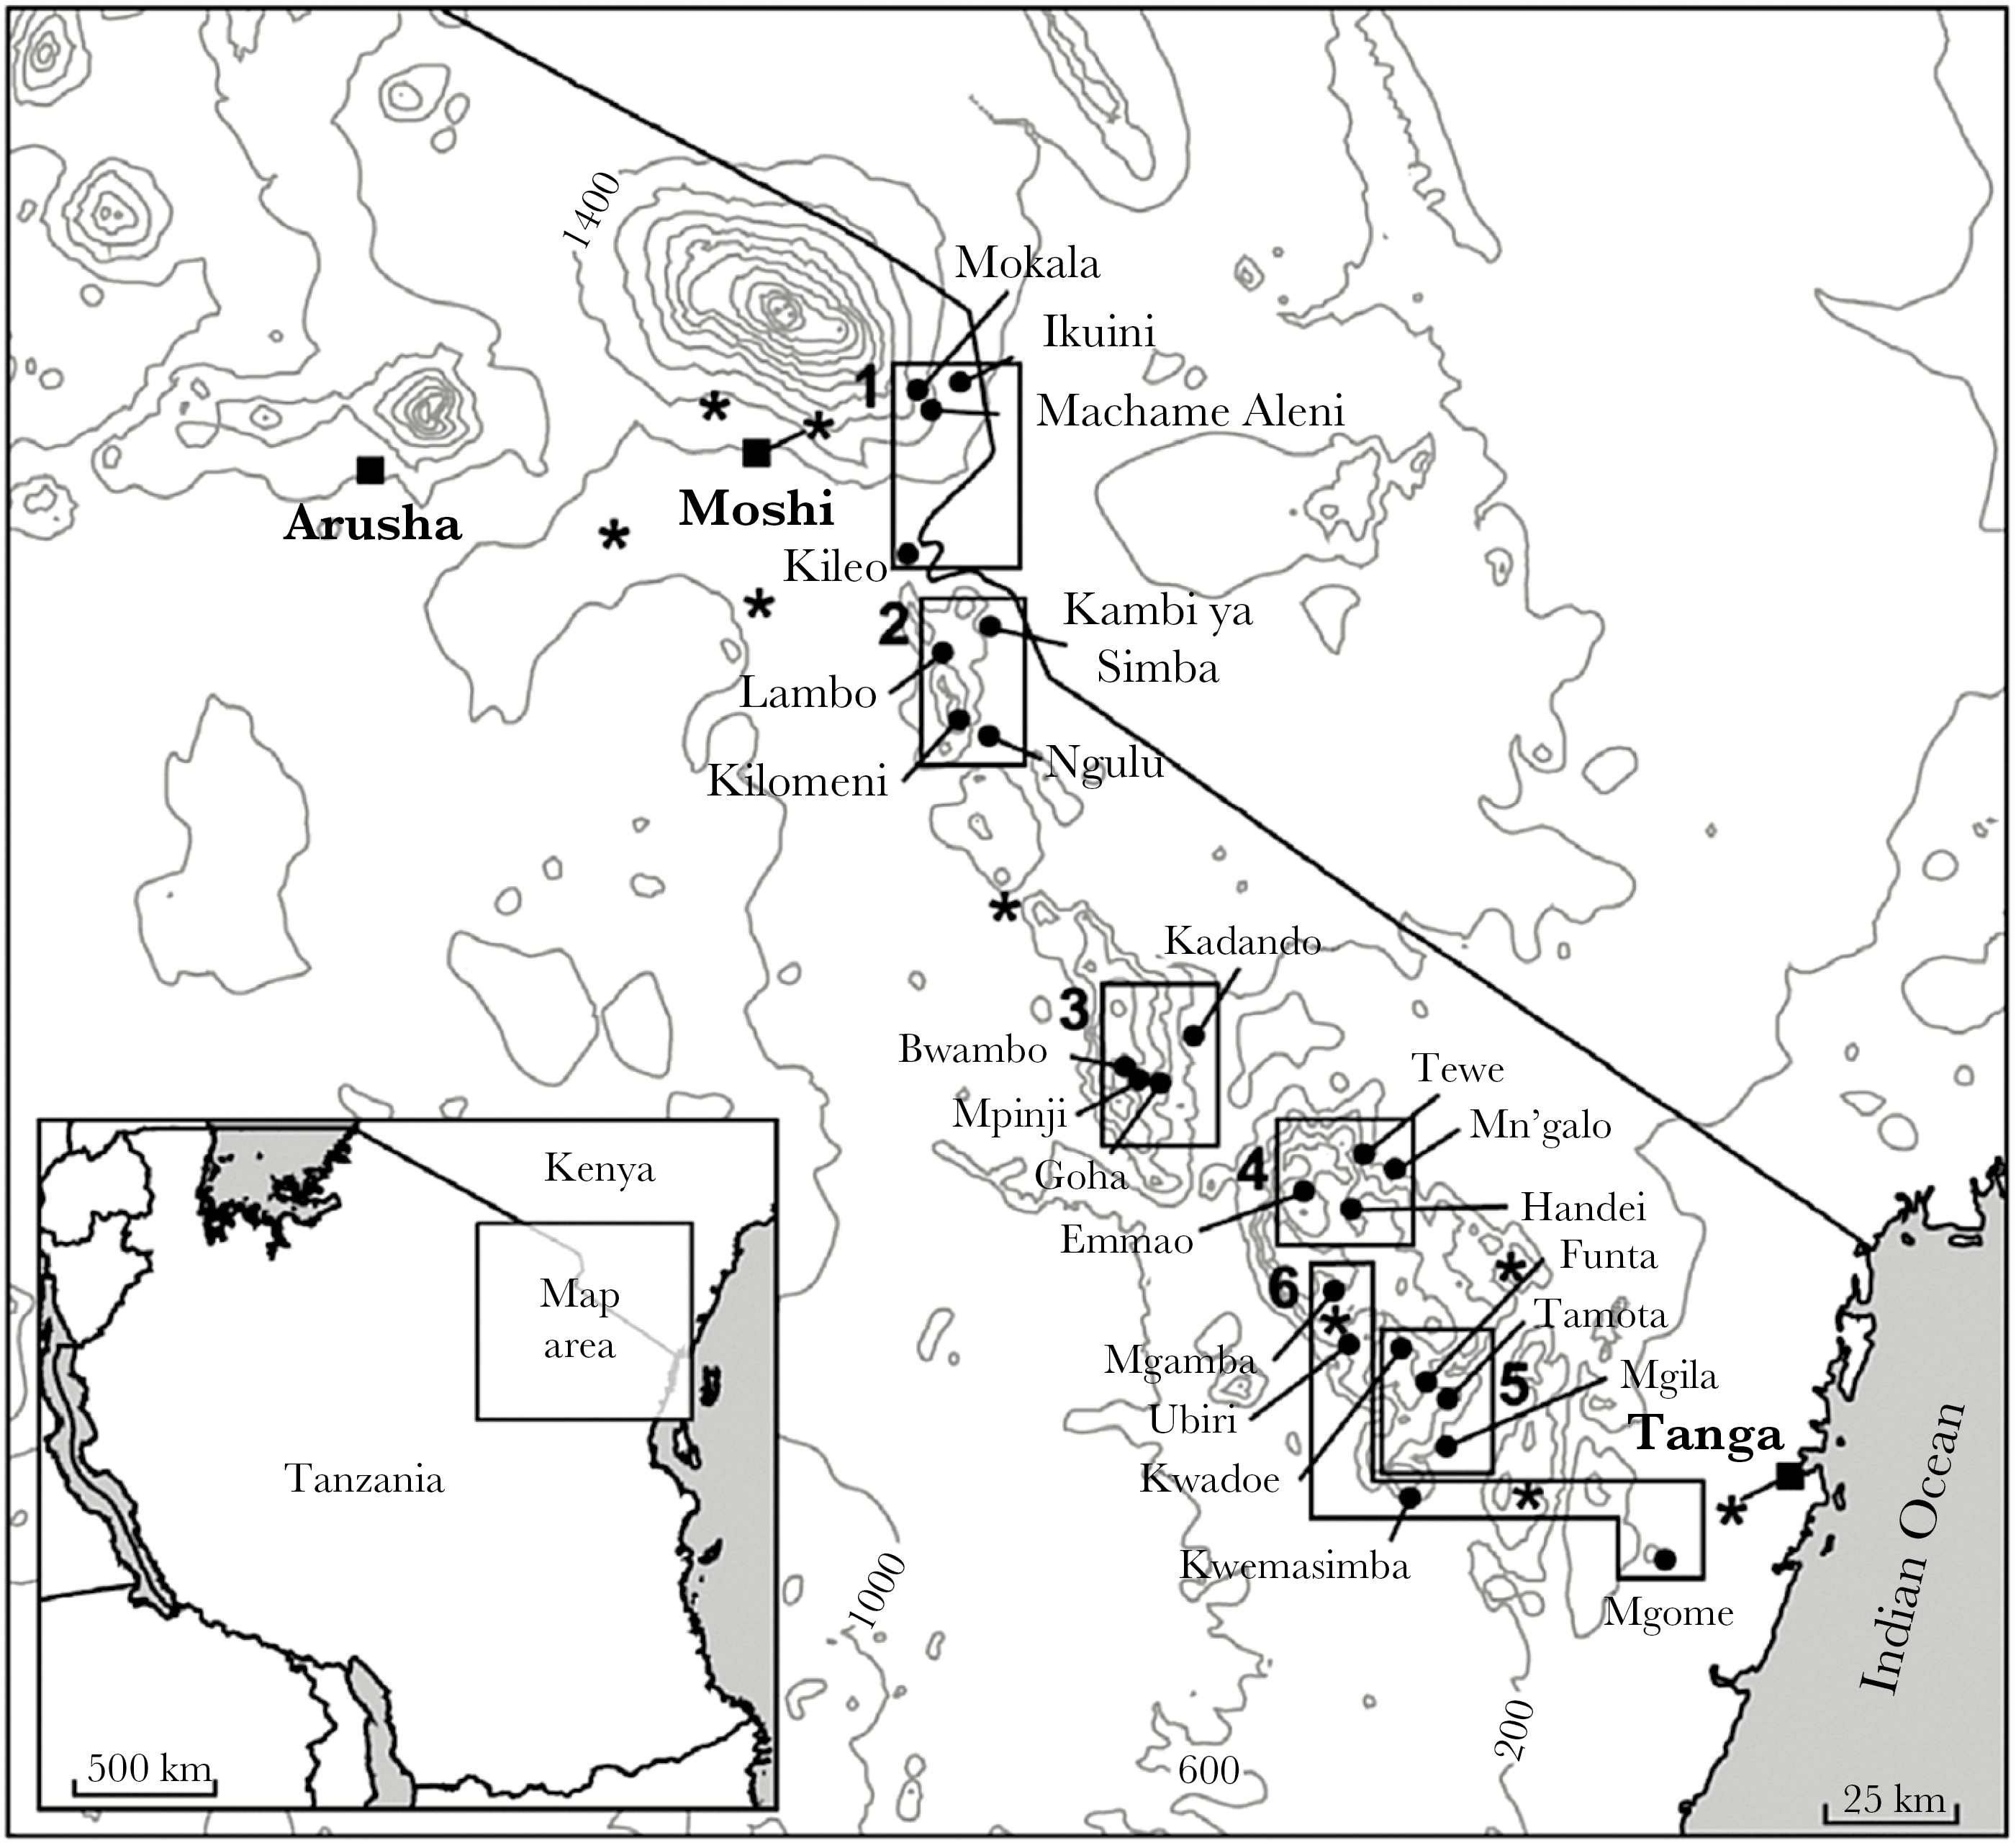
\includegraphics[width=13cm]{images/site_map.jpeg}
\caption[Map of study sites]{Map of study sites (black circles) grouped by respective numbered region transects: Rombo (transect 1), North Pale (transect 2), South Pale (transect 3), West Usambara 1 (transect 4), West Usambara 2 (transect 5), and West Usambara 3 (transect 6).
Locations of the 8 meteorological stations are also shown (asterisks).
Reprinted with permission \cite{sepulveda2017malaria}.}
\label{fig:tanzania.map}
\end{figure}



%%%%%%%%%%%%%%%%%%%%%%%%%
% VARIABLES DESCRIPTION %
%%%%%%%%%%%%%%%%%%%%%%%%%

%\section{Descriptive analysis}
\section{Variables description}

To study transmission intensity amongst Tanzania's different populations, several variables were selected to be analysed in this thesis.
Some variables refer the demographical information collected regarding each site.
For each village, its mean altitude and encompassing transect were registered.
Variables that characterise the selected inhabitants were also used.
Firstly, the infection outcome recorded for each individual.
This variable has value 0 in absence of infection and 1 when presence of malaria parasites is found, indicating the assumed true individual status.
Other binary variables selected were the gender of each individual (as female or male), and the three \textit{P. falciparum} antigens (either present or absent), used here as serological markers to identify exposure to parasite instead of immunological protection.
Since each antigen has different response levels to the presence of \textit{P. falciparum} parasites, the comparison of their serological outcomes under the same study characteristics could help to better understand how transmission intensity varies across the different villages.
Ethnicities were also recorded, with four possible ethnic groups: Wachaga, Wapare, Wasambaa, and Other.
As mentioned in the previous section, the ethnic groups of each village are expected to represent the genetic variability seen in each transect.
In other words, in each transect an ethnic group dominated the others in proportion.
The age in years of every individual was also a recorded variable, as well as the respective age group each one belonged to, with three possible categories, 1$-$4, 5$-$14, and 15$-$45.

Depending on the study objective, more than one of the described variables can be classified as the desired response variable, with others being used as explanatory variables and potential risk factors.
An example of response variable can be the infection or serological status of each individual.
The binary outcomes of these variables can be used to calculate the number of infected or previously exposed individuals within each village, attending other particular variables that may characterise such response.
All ten variables considered for the analyses are listed below.
%\subsubsection{Outcomes of interest}
%To study the transmission intensity amongst Tanzania's population, the response variable used was the number of infected individuals at each age group.
%This variable is dependent on the outcome for \textit{P. falciparum} infection, with possible values 0 in absence of infection and 1 when presence of malaria parasites is found.
%The outcome indicates the assumed true individual status.
%The use of this variable has a direct use when estimating malaria transmission intensity via the more classical epidemiological measures.
%\textbf{falar também das serologias!}
%\subsubsection{Covariates}
%Alongside the infection status a number of potential explanatory variables were recorded for each individual.
%These covariates can be separated in two distinct groups regarding the information they contain: demographical variables and epidemiological variables.
%The demographical variables the all the information collected regarding the sites and its inhabitants.
%Included in this group are the mean altitude of each village, the different transects, the three age groups, the individuals' gender, and their respective ethnicity.
%The epidemiological variables refer the three specific \textit{P. falciparum} antigens screened: PfMSP1, PfMSP2, and PfAMA1.
%Similar to the infection status, the epidemiological variables were registered for all individuals as 0 when it is not detectable, and 1 if it is.
%The explanatory variables used in the analyses are briefly listed listed below.
%\setlist[description]{font=\normalfont\itshape\space, leftmargin=\parindent,labelindent=\parindent}
%
\setlist[description]{labelindent=0pt,style=multiline,leftmargin=1.9cm}
\begin{description}[font=\normalfont\itshape]
\item [Altitude:]  Mean altitude of each village, in meters;
\item [Transect:]  Transect of villages (categorical variable with six possible outcomes, Rombo, North Pare, South Pare, West Usambara 1, West Usambara 2, and West Usambara 3);
\item [Gender:]  Gender of each individual (binary variable with possible outcomes, Female and Male);
\item [EthGp:]  Ethnic group of each individual (categorical variable with four possible outcomes, Wachaga, Wapare, Wasambaa, and Other);
\item [AgeYears:]  Age of each individual, in years;
\item [AgeGp:]  Age group of each individual (categorical variable with three possible outcomes, 1$-$4, 5$-$14, and 15$-$45);
\item [Infection:]  Infection status of each individual (binary variable with possible outcomes, 0 = infection is absent, and 1 = \textit{P. falciparum} malaria detected);
\item [MSP1:]  Serological status regarding the antigen MSP1 (binary variable with possible outcomes, 0 = antigen absent in serum, and 1 = antigen detected);
\item [MSP2:]  Serological status regarding the antigen MSP2 (binary variable with possible outcomes, 0 = antigen absent in serum, and 1 = antigen detected);
\item [AMA1:]  Serological status regarding the antigen AMA1 (binary variable with possible outcomes, 0 = antigen absent in serum, and 1 = antigen detected).
\end{description}

%%%%%%%%%%%%%%%%%%%%%%%%
% EXPLORATORY ANALYSIS %
%%%%%%%%%%%%%%%%%%%%%%%%
\section{Exploratory analysis}

The decision to perform analyses using only the complete cases for the described variables led to the exclusion of three villages from the West Usambara 3 transect (the villages removed were Magamba, Ubiri and Kwemasimba), where serological samples were not collected.
In this transect the remaining village, Mgome, is a coastal village with the lowest recorded mean altitude, at 179 meters.
By comparison, the first transect of the Usambara mountains registers the village located at highest altitude, Emmao, at 1780 meters high.
The resulting total population sample size is 5058 individuals, separated across the 21 villages (Table \ref{tab:demographic}).
Considering each village, the sample sizes ranged from 53 (Ngulu) up to 379 individuals (Handei).
Even with different sample sizes it was possible to verify the attention taken by the study to maintain a similar structure for ages and genders, as these variables presented similar proportions across all sites.
Similar attention was also taken for the different ethnic groups within each one of the six transects.
Each transect had a dominant ethnicity.
Rombo was represented by the Wachaga ethnic group, having only one village (Kileo) with Wapare as the main ethnicity, North and South Pare had mostly individuals from the Wapare ethnic group, both West Usambara 1 and 2 had Wasambaa as the main ethnic group, and the last transect, West Usambara 3, represented a mixture of different ethnicities (Other).
\\

\begin{table}[ht!]
\centering
\caption[Variables recorded for each village]{Descriptive table with the recorded variables for each one of the 21 selected villages within six different transects.
For all villages, values for mean altitude, population sample size, gender proportion, mean age, and proportion of each ethnic group are presented.}
\label{tab:demographic}
\begin{adjustbox}{width=1\linewidth}
\begin{tabular}{llccrcrrrr} 
\toprule
\multicolumn{1}{c}{\multirow{2}{*}{Transect}} & \multicolumn{1}{c}{\multirow{2}{*}{Village}} & \multirow{2}{*}{\begin{tabular}[c]{@{}c@{}} Altitude,\\m\end{tabular}} & \multirow{2}{*}{$n$} & \multirow{2}{*}{\begin{tabular}[c]{@{}c@{}} Female\\proportion, \% ($n$)\end{tabular}} & \multirow{2}{*}{\begin{tabular}[c]{@{}c@{}} Mean age,\\years\end{tabular}} & \multicolumn{4}{c}{Ethnic group, \% ($n$)}  \\ 
\cmidrule{7-10}
                          & \multicolumn{1}{c}{}   &   &   &   &   &   \multicolumn{1}{c}{Wachaga}   &   \multicolumn{1}{c}{Wapare}   &   \multicolumn{1}{c}{Wasambaa}   &   \multicolumn{1}{c}{Other}   \\ 
\midrule
Rombo                     &   Mokala          &   1703   &   291   &   62.20 (181)   &   15.34   &   98.28 (286)&   0.00 (0)    &   0.00 (0)   &   1.72 (5)     \\
                          &   Machame Aleni   &   1422   &   225   &   55.11 (124)   &   15.28   &   100.00 (225)  &   0.00 (0)    &   0.00 (0)   &   0.00 (0)   \\
                          &   Ikuini          &   1160   &   256   &   57.03 (146)   &   14.99   &   98.83 (253)&   0.39 (1)    &   0.39 (1)    &   0.39 (1)     \\
                          &   Kileo           &   723    &   223   &   61.88 (138)   &   14.94   &   3.14 (7)   &   86.55 (193) &   5.38 (12)   &   4.93 (11)    \\
\cmidrule{2-10}
N. Pare                   &   Kilomeni        &   1556   &   101   &   55.45 (56)    &   17.71   &   0.99 (1)   &   96.04 (97)  &   0.99 (1)    &   1.98 (2)     \\
                          &   Lambo           &   1188   &   131   &   64.89 (85)    &   15.43   &   0.00 (0)   &   94.66 (124) &   1.53 (2)    &   3.82 (5)     \\
                          &   Ngulu           &   832    &   53    &   52.83 (28)    &   13.75   &   1.89 (1)   &   96.23 (51)  &   1.89 (1)    &   0.00 (0)   \\
                          &   Kambi ya Simba  &   746    &   93    &   50.54 (47)    &   15.43   &   6.45 (6)   &   81.72 (76)  &   0.00 (0)   &   11.83 (11)   \\
\cmidrule{2-10}
S. Pare                   &   Bwambo          &   1598   &   240   &   54.17 (130)   &   16.61   &   1.25 (3)   &   98.33 (236  &   0.00 (0)   &   0.42 (1)     \\
                          &   Mpinji          &   1445   &   198   &   63.13 (125)   &   14.03   &   0.51 (1)   &   93.94 (186) &   2.02 (4)    &   3.54 (7)     \\
                          &   Goha            &   1163   &   337   &   58.75 (198)   &   14.53   &   0.00 (0)   &   96.44 (325) &   2.97 (10)   &   0.59 (2)     \\
                          &   Kadando         &   528    &   281   &   59.07 (166)   &   16.19   &   1.42 (4)   &   69.40 (195) &   18.51 (52)  &   10.68 (30)   \\
\cmidrule{2-10}
W. Usamb. 1               &   Emmao           &   1780   &   170   &   61.18 (104)   &   16.04   &   0.00 (0)   &   15.29 (26)  &   60.00 (102) &   24.71 (42)   \\
                          &   Handei          &   1368   &   379   &   56.46 (214)   &   14.21   &   0.00 (0)   &   2.11 (8)    &   94.20 (357) &   3.69 (14)    \\
                          &   Tewe            &   999    &   326   &   61.96 (202)   &   15.68   &   0.31 (1)   &   3.07 (10)   &   93.56 (305) &   3.07 (10)    \\
                          &   Mn'galo         &   389    &   363   &   58.95 (214)   &   15.58   &   0.00 (0)   &   1.10 (4)    &   89.53 (325) &   9.37 (34)    \\
\cmidrule{2-10}
W. Usamb. 2               &   Kwadoe          &   1564   &   296   &   62.16 (184)   &   15.14   &   0.68 (2)   &   2.03 (6)    &   94.59 (280) &   2.70 (8)     \\
                          &   Funta           &   1240   &   252   &   66.67 (168)   &   15.90   &   0.40 (1)   &   0.40 (1)    &   96.43 (243) &   2.78 (7)     \\
                          &   Tamota          &   1055   &   330   &   53.94 (178)   &   15.62   &   0.61 (2)   &   1.21 (4)    &   94.55 (312) &   3.64 (12)    \\
                          &   Mgila           &   375    &   288   &   71.88 (207)   &   15.62   &   0.00 (0)   &   9.72 (28)   &   67.36 (194) &   22.92 (66)   \\
\cmidrule{2-10}
W. Usamb. 3               &   Mgome           &   179    &   225   &   54.22 (122)   &   15.46   &   0.44 (1)   &   5.33 (12)   &   9.78 (22)   &   84.44 (190)  \\
\bottomrule
\end{tabular}
\end{adjustbox}
\end{table}

The combination of characteristics from each site may have different impacts in the resulting prevalence of infection, changing the seroprevalence values as consequence (Table \ref{tab:prevalence.categories}).
The overall prevalence of infection was reported as 19.81\%, with seroprevalence values for MSP1, MSP2, and AMA1 being 36.22\%, 40.25\%, and 46.56\%, respectively.
% The confidence intervals for the prevalence and seroprevalence values represent the uncertainty based on the sample size at each category, calculated for a significance level fixed at 0.05.
Analysing the different categories showed that \textit{Gender} did not seem to pose an effect on neither prevalence nor seroprevalence, as both estimates did not change much from female individuals to males.
Prevalence of infection across ethnic groups (variable \textit{EthGp}), showing different registered sample sizes, suggested mixed ethnicities ($\textit{EthGp}_{Other}$) suffered the most from detectable cases, presenting higher seroprevalence levels as well.
% As previously described, this ethnic group represents the last of the West Usambara transects, with only the village of Mgome.

% The change in prevalence across different age groups (\textit{AgeGp}) suggests evidence for the previously referred peak-shift effect.
% A justification might be the gradual increase in seroprevalence from one age group to the following.
Since individuals are born almost immunologically unprotected, with only maternal antibodies inherited from the mother, the first age group ($\textit{AgeGp}_{1-4}$) showed lower seroprevalence values.
Contrarily, the last age group ($AgeGp_{15-45}$) had a reduced prevalence of infection, with over 50\% of this older population showing presence of the various antimalarial antigens.
In this particular scenario, the difference in prevalence and seroprevalence between age groups might be justified by the gradual accumulation of protective antibodies due to exposure over time.
The primary risk group in these African populations is then children younger than 5 years old, who have yet to develop an efficient immune system \cite{snow2002consequences}.
Pregnant woman can also be a vulnerable group to malaria infections, as pregnancy affects the immune system's defences against the disease \cite{carter2002evolutionary,perlmann2002malaria}.
This influence of age on prevalence of infection and seroprevalence can be seen as the previously described peak-shift.
As malaria does not produce long-lasting immunity, in a case of transmission intensity reduction (or eradication), the developed (and accumulated) antibodies for the specific antigens could gradually decay, with the immunologically protected individuals becoming susceptible to high and symptomatic cases of infection, once again.

\begin{table}[H]
\centering
\caption[Prevalence and seroprevalence for each categorical variable]{Prevalence and seroprevalence of each one of the specific \textit{P. falciparum} antigens, estimated for the categorised available variables. Each prevalence and seroprevalence shows the 95\% confidence interval (CI), estimated using the Wald interval.}
\label{tab:prevalence.categories}
\begin{adjustbox}{width=1\linewidth}
\begin{tabular}{llcrrrr} 
\toprule
\multicolumn{1}{c}{\multirow{2}{*}{Variables}} & \multicolumn{1}{c}{\multirow{2}{*}{Categories}} & \multicolumn{1}{c}{\multirow{2}{*}{$n$}} & \multicolumn{1}{c}{\multirow{2}{*}{\begin{tabular}[c]{@{}c@{}}Prevalence, \%\\ (95\% CI) \end{tabular}}} & \multicolumn{3}{c}{Seroprevalence, \% (95\% CI)}                                \\ 
\cmidrule{5-7}
\multicolumn{1}{c}{} & \multicolumn{1}{c}{} & \multicolumn{1}{c}{} & \multicolumn{1}{c}{} & \multicolumn{1}{c}{MSP1} & \multicolumn{1}{c}{MSP2} & \multicolumn{1}{c}{AMA1}  \\ 
\midrule
\textit{AgeGp}                                 & 1$-$4         &   1261   & 19.59 (17.40, 21.78)   & 19.83 (17.63, 22.03)   & 24.27 (21.90, 26.63)   & 30.61 (28.07, 33.15)   \\
                                               & 5$-$14        &   1789   & 25.88 (23.85, 27.91)   & 30.58 (28.44, 32.71)   & 39.18 (36.92, 41.45)   & 45.78 (43.47, 48.09)   \\
                                               & 15$-$45       &   2008   & 14.54 (13.00, 16.08)   & 51.54 (49.36, 53.73)   & 51.25 (49.06, 53.43)   & 57.27 (55.11, 59.43)   \\
\textit{Gender}                                & Female      &   3017   & 18.99 (17.59, 20.39)   & 38.88 (37.14, 40.62)   & 42.46 (40.70, 44.22)   & 47.99 (46.21, 49.78)   \\
                                               & Male        &   2041   & 21.02 (19.25, 22.79)   & 32.29 (30.26, 34.32)   & 36.99 (34.90, 39.09)   & 44.44 (42.28, 46.59)   \\
\textit{EthGp}                                 & Wachaga     &   794    & 6.68 (4.94, 8.41)      & 20.03 (17.24, 22.81)   & 4.28 (2.87, 5.69)      & 7.68 (5.83, 9.54)      \\
                                               & Wapare      &   1583   & 9.85 (8.39, 11.32)     & 34.30 (31.96, 36.64)   & 39.48 (37.07, 41.89)   & 47.38 (44.92, 49.84)   \\
                                               & Wasambaa    &   2223   & 28.39 (26.51, 30.26)   & 38.46 (36.44, 40.48)   & 48.13 (46.06, 50.21)   & 55.29 (53.22, 57.35)   \\
                                               & Other       &   458    & 35.37 (30.99, 39.75)   & 60.04 (55.56, 64.53)   & 67.03 (62.73, 71.34)   & 68.78 (64.53, 73.02)   \\
\textit{Transect}                              & Rombo       &   995    & 6.73 (5.18, 8.29)      & 31.26 (28.38, 34.14)   & 4.82 (3.49, 6.16)      & 10.35 (8.46, 12.24)    \\
                                               & N. Pare     &   378    & 4.76 (2.62, 6.91)      & 28.31 (23.77, 32.85)   & 38.36 (33.46, 43.26)   & 54.23 (49.21, 59.26)   \\
                                               & S. Pare     &   1056   & 11.74 (9.80, 13.68)    & 29.64 (26.89, 32.39)   & 45.17 (42.17, 48.17)   & 49.91 (46.89, 52.92)   \\
                                               & W. Usamb. 1 &   1238   & 32.31 (29.71, 34.92)   & 29.08 (26.55, 31.61)   & 40.39 (37.65, 43.12)   & 65.75 (63.11, 68.39)   \\
                                               & W. Usamb. 2 &   1166   & 23.93 (21.48, 26.38)   & 46.83 (43.96, 49.69)   & 56.69 (53.85, 59.53)   & 42.97 (40.13, 45.81)   \\
                                               & W. Usamb. 3 &   225    & 50.67 (44.13, 57.20)   & 86.67 (82.22, 91.11)   & 91.11 (87.39, 94.83)   & 91.11 (87.39, 94.83)   \\
Overall                           & \multicolumn{1}{c}{--}   &   5058   & 19.81 (18.71, 20.91)   & 36.22 (34.90, 37.54)   & 40.25 (38.90, 41.60)   & 46.56 (45.19, 47.93)   \\
\bottomrule
\end{tabular}
\end{adjustbox}
\end{table}
\newpage

% \textcolor{red}{EM BAIXO RETIRAR/MELHORAR IMMUNOGENICITY E SINÓNIMOS}
When analysing the prevalence for each village, the infection outcome varied from 0.89\% in Machame Aleni, to 50.67\% in Mgome (Table \ref{tab:prevalence.seroprevalence}).
Since villages within each transect were ordered by decreasing altitude, it was possible to see an apparent pattern for prevalence of infection.
Villages located at higher altitudes seemingly had lower prevalence of infection than villages at lower altitudes.
As climate changes with altitude, sites with lower temperature or humidity values (that do not suit the \textit{Anopheles} mosquitoes) tend to present lower prevalence estimates \cite{lindsay1996climate}.
This impact on maximum reachable prevalence of infection allows altitude to be considered a proxy for malaria transmission intensity.

The sero-epidemiological variables were related to altitude as well, with seroprevalence appearing as a direct response to infection, since the gradient of immunological responses depends on the level of exposure to the parasite.
For the same village, the three antigens analysed presented different seroprevalence values, confirming their different immunogenic profiles when close to the same parasites and corroborating the idea that using more than a single antigen could be useful to better understanding the heterogeneity in malaria transmission intensity.
Of all, AMA1 appeared the most sensitive to \textit{P. falciparum}, with higher seroprevalence even at low altitude villages, when compared to the remaining two.
Seroprevalence estimates for the MSP1 antigen tend to be the lowest, at times presenting similar outcomes as MSP2.
All seroprevalence values appear to correlate well with prevalence of infection.
% However, the three are acknowledged for their sensitivity over their immunological protective capabilities, being generally used as indicators for parasite exposure \cite{reddy2012high,ondigo2014estimation}.
% one can help to predict malaria transmission intensity.
\\

\makeatletter
\setlength{\@fptop}{0pt}
\begin{table}[ht!]
\centering
\caption[Prevalence and seroprevalence of each village]{Values of prevalence and seroprevalence of each one of the specific \textit{P. falciparum} antigens, estimated for each village and their respective 95\% confidence interval (CI), estimated using the Wald interval. Proportions are based on the number of individuals in each village, column $n$ from previous Table \ref{tab:demographic}.}
\begin{adjustbox}{width=1\linewidth}
\label{tab:prevalence.seroprevalence}
\begin{tabular}{llrrrr} 
\toprule
\multicolumn{1}{c}{\multirow{2}{*}{Transect}} & \multicolumn{1}{c}{\multirow{2}{*}{Village~}} &
\multirow{2}{*}{\begin{tabular}[c] {@{}c@{}}Prevalence, \%\\(95\% CI)\end{tabular}} & \multicolumn{3}{c}{Seroprevalence, \% (95\% CI)}  \\ 
\cmidrule{4-6}
                          & \multicolumn{1}{c}{}   &   & \multicolumn{1}{c}{MSP1}   & \multicolumn{1}{c}{MSP2}   &   \multicolumn{1}{c}{AMA1} \\ 
\midrule
Rombo                     &   Mokala          &   5.84 (3.15, 8.54)      & 15.46 (11.31, 19.62)   & 3.09 (1.10, 5.08)      & 6.53 (3.69, 9.37)      \\
                          &   Machame Aleni   &   0.89 (0.00, 2.12)      & 24.44 (18.83, 30.06)   & 3.11 (0.84, 5.38)      & 4.00 (1.44, 6.56)      \\
                          &   Ikuini          &   12.89 (8.79, 17.00)    & 17.97 (13.27, 22.67)   & 1.95 (0.26, 3.65)      & 7.81 (4.53, 11.10)     \\
                          &   Kileo           &   6.73 (3.44, 10.01)     & 73.99 (68.23, 79.75)   & 12.11 (7.83, 16.39)    & 24.66 (19.01, 30.32)   \\
\cmidrule{2-6}
N. Pare                   &   Kilomeni        &   1.98 (0.00, 4.70)      & 8.91 (3.35, 14.47)     & 8.91 (3.35, 14.47)     & 23.76 (15.46, 32.06)   \\
                          &   Lambo           &   2.29 (0.00, 4.85)      & 19.85 (13.02, 26.68)   & 21.37 (14.35, 28.39)   & 54.20 (45.67, 62.73)   \\
                          &   Ngulu           &   3.77 (0.00, 8.90)      & 52.83 (39.39, 66.27)   & 81.13 (70.60, 91.67)   & 84.91 (75.27, 94.54)   \\
                          &   Kambi ya Simba  &   11.83 (5.26, 18.39)    & 47.31 (37.16, 57.46)   & 69.89 (60.57, 79.22)   & 69.89 (60.57, 79.22)   \\
\cmidrule{2-6}
S. Pare                   &   Bwambo          &   5.00 (2.24, 7.76)      & 8.33 (4.84, 11.83)     & 47.50 (41.18, 53.82)   & 33.33 (27.37, 39.30)   \\
                          &   Mpinji          &   2.53 (0.34, 4.71)      & 6.06 (2.74, 9.38)      & 55.05 (48.12, 61.98)   & 44.44 (37.52, 51.37)   \\
                          &   Goha            &   11.57 (8.16, 14.99)    & 28.49 (23.67, 33.31)   & 38.58 (33.38, 43.77)   & 53.41 (48.09, 58.74)   \\
                          &   Kadando         &   24.20 (19.19, 29.21)   & 65.84 (60.29, 71.38)   & 44.13 (38.32, 49.93)   & 63.70 (58.08, 69.32)   \\
\cmidrule{2-6}
W. Usamb. 1               &   Emmao           &   2.94 (0.40, 5.48)      & 1.76 (0.00, 3.74)      & 1.18 (0.00, 2.80)      & 13.53 (8.39, 18.67)    \\
                          &   Handei          &   27.97 (23.45, 32.49)   & 18.21 (14.32, 22.09)   & 35.36 (30.54, 40.17)   & 68.07 (63.38, 72.77)   \\
                          &   Tewe            &   33.74 (28.61, 38.88)   & 30.06 (25.08, 35.04)   & 44.17 (38.78, 49.56)   & 64.42 (59.22, 69.61)   \\
                          &   Mn'galo         &   49.31 (44.17, 54.45)   & 52.34 (47.20, 57.48)   & 60.61 (55.58, 65.63)   & 88.98 (85.76, 92.20)   \\
\cmidrule{2-6}
W. Usamb. 2               &   Kwadoe          &   7.09 (4.17, 10.02)     & 9.12 (5.84, 12.40)     & 16.89 (12.62, 21.16)   & 21.62 (16.93, 26.31)   \\
                          &   Funta           &   24.60 (19.29, 29.92)   & 61.51 (55.50, 67.52)   & 64.68 (58.78, 70.58)   & 51.19 (45.02, 57.36)   \\
                          &   Tamota          &   26.06 (21.32, 30.80)   & 49.09 (43.70, 54.48)   & 63.03 (57.82, 68.24)   & 32.42 (27.37, 37.47)   \\
                          &   Mgila           &   38.19 (32.58, 43.81)   & 70.14 (64.85, 75.42)   & 83.33 (79.03, 87.64)   & 69.79 (64.49, 75.09)   \\
\cmidrule{2-6}
W. Usamb. 2               &   Mgome           &   50.67 (44.13, 57.20)   & 86.67 (82.22, 91.11)   & 91.11 (87.39, 94.83)   & 91.11 (87.39, 94.83)   \\
\bottomrule
\end{tabular}
\end{adjustbox}
\end{table}
\makeatother

























%
\chapter{Description of data}

%%%%%%%%%%%%
%%% 2.1) %%%
%%%%%%%%%%%%
\section{Tanzania data set}

\subsection{Study site}

Data were collected as part of a program investigating the burden of the disease and its' transmission intensity, with several demographic and populational indices gathered to study and possibly predict the intensity of malaria transmission \cite{drakeley2005altitude}. The study area ranged from the highest mountain in Africa -- Mt. Kilimanjaro -- to Tanga, a coastal plain of North-East Tanzania (figure \ref{fig:2.1}). In this delimited region, six transects were defined based on the altitude -- 3 in the Kilimanjaro region, and 3 in the Tanga region -- each one containing four villages, one at high altitude ($>$1200m), two at intermediate altitude (600m$-$1200m), and one the closest to a low altitude ($<$600m), chosen to represent areas of varying transmission intensity, based on the premise that an effect of increasing altitude follows a reduction in vectors density \cite{bodker2003relationship}. For each village a selection criteria was used to minimise differences within transects in ethnicity, seasonal migration or access to health care.

% IS IT WORTH IT TO WRITE THIS PARAGRAPH?
According to the source article \cite{drakeley2005altitude}, the study area was mapped making use of differential global positioning satellite techniques (Trimble GeoExplorer III and Pro XR receivers; Trimble Navigation), and geographical data were analysed by use of Arc/Info~7.1 and ArcView~3.2 (ESRI). The long-term average daily mean temperature was derived from meteorological stations across both regions and rainfall estimates were derived by Meteosat infrared data collected by the Climate Prediction Center at the US National Oceanographic and Atmospheric Administration.

\begin{figure}[ht!]
\center
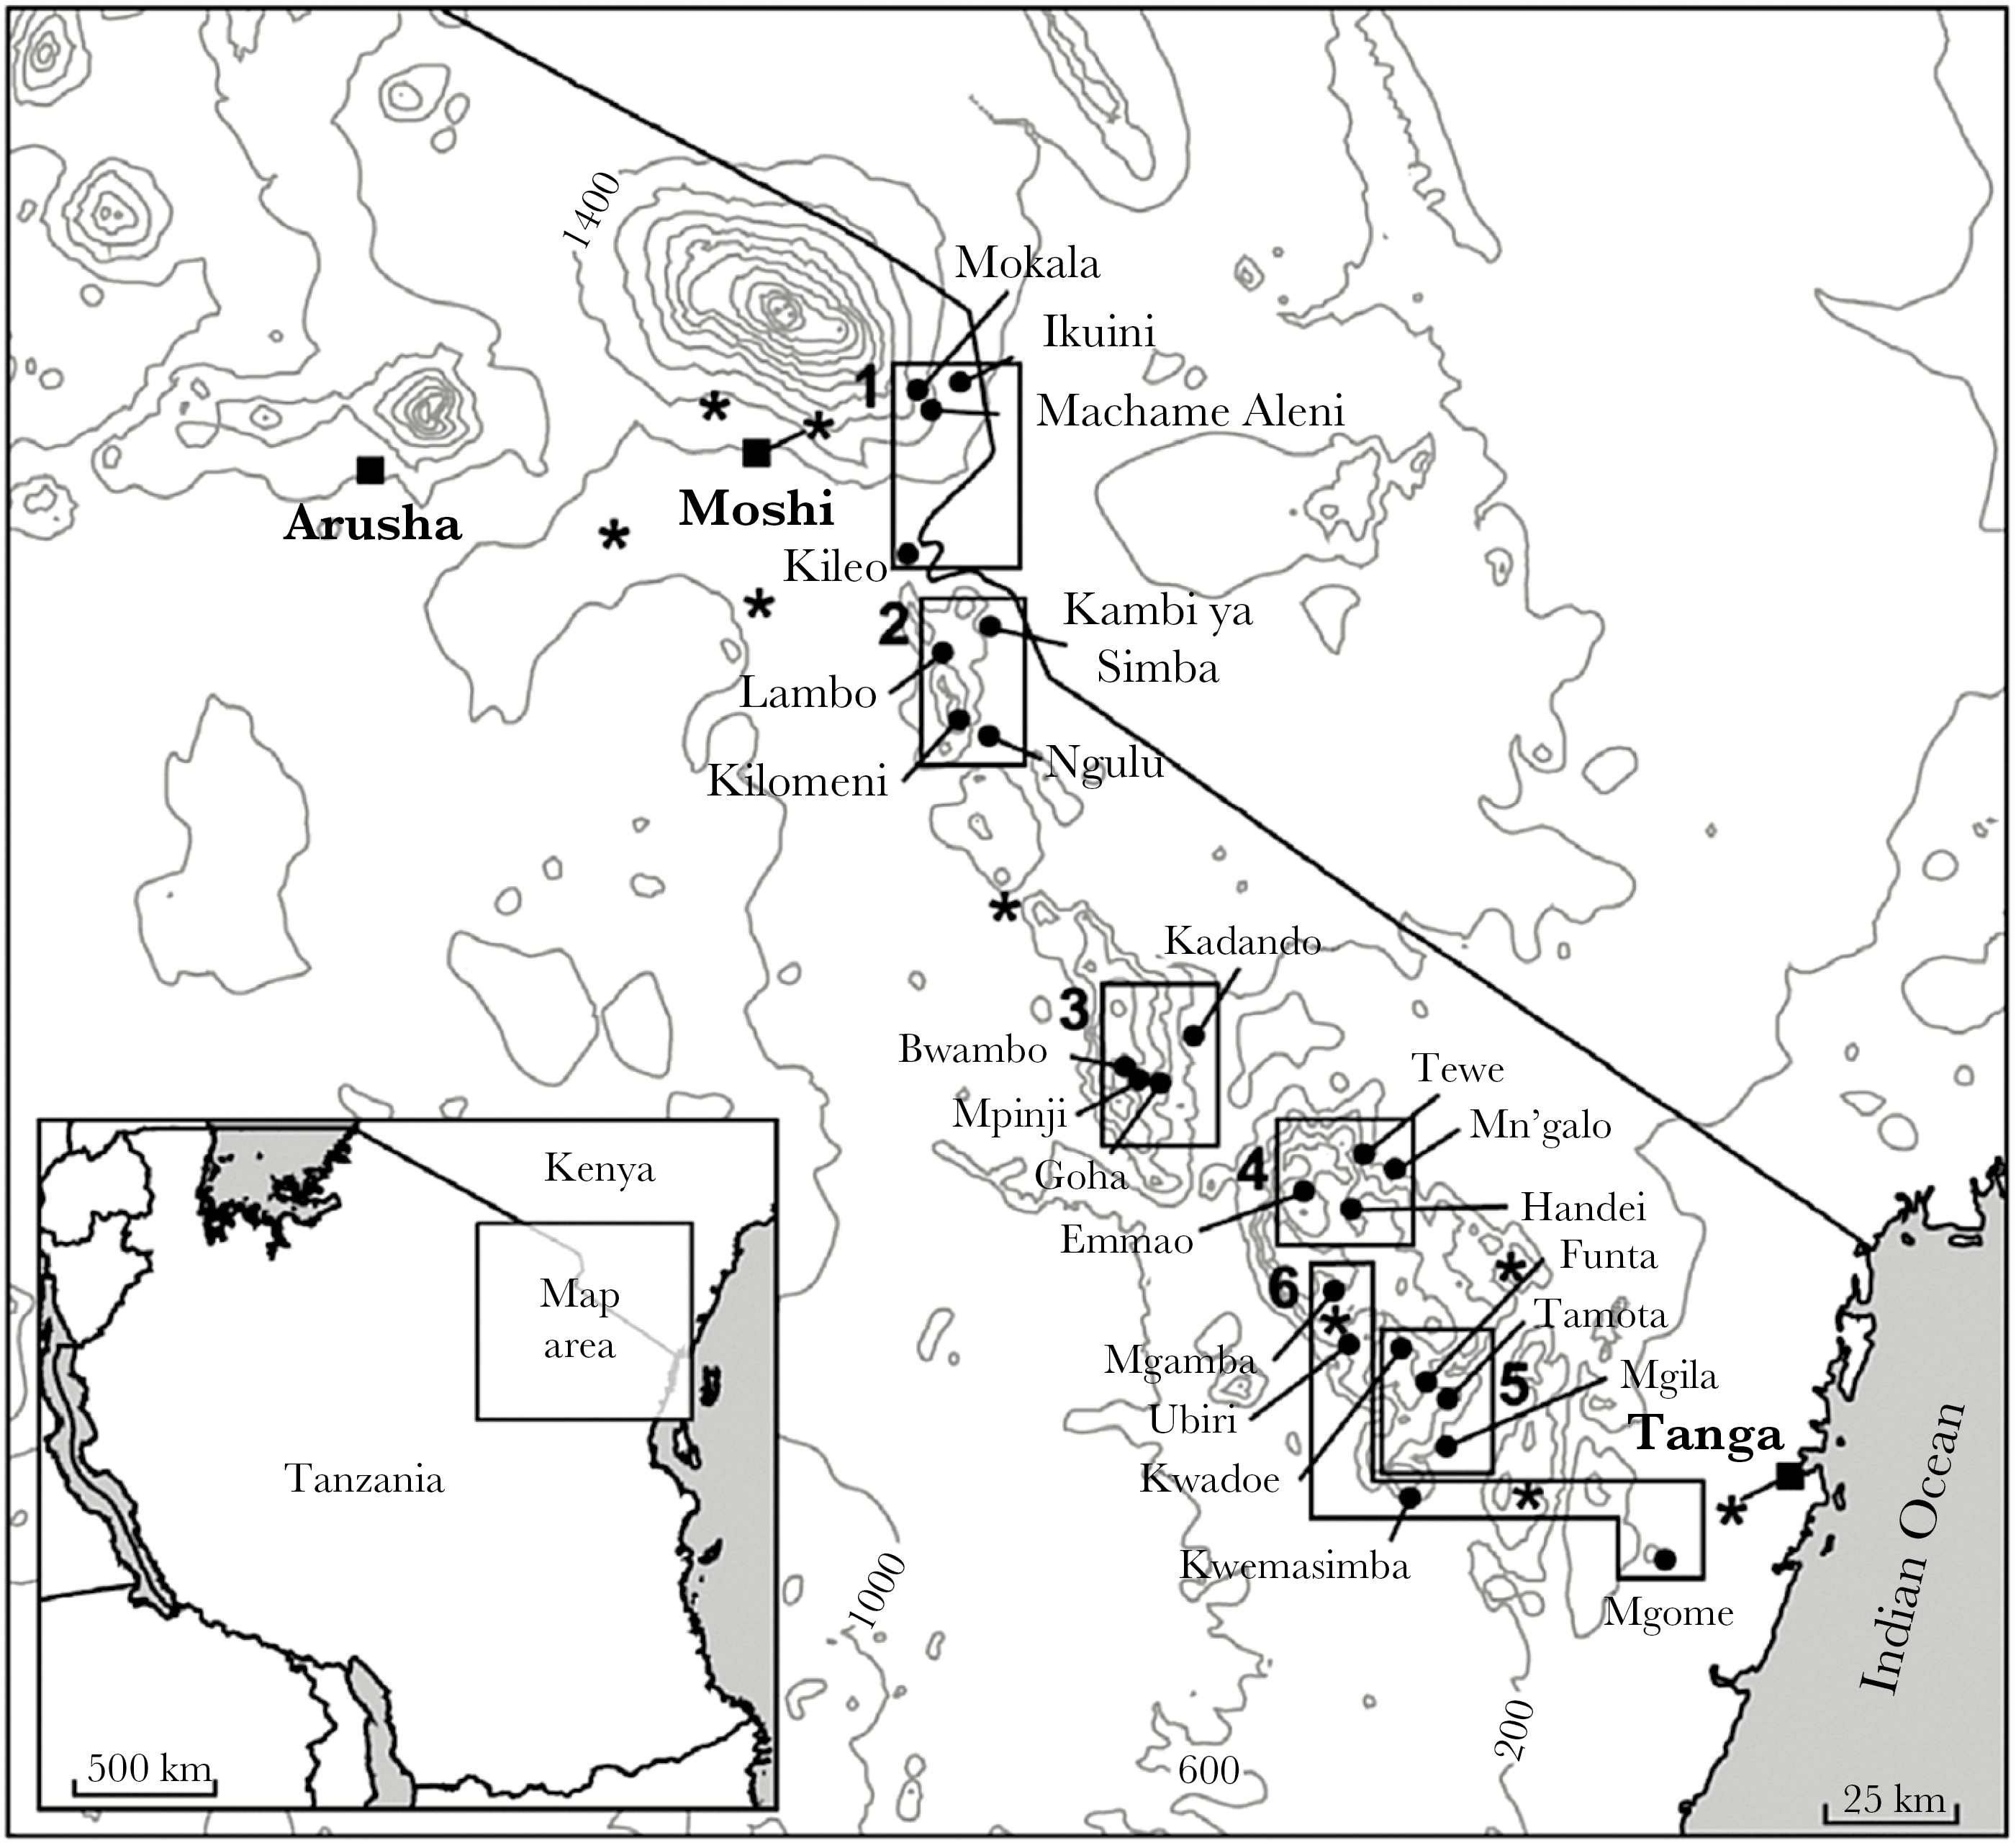
\includegraphics[width=13cm]{images/site_map.jpeg}
\caption[Map of study sites]{Map of study sites (black circles) grouped by respective numbered region transects: Rombo (transect 1), North Pale (transect 2), South Pale (transect 3), West Usambara 1 (transect 4), West Usambara 2 (transect 5) and West Usambara 3 (transect 6). Locations of the 8 meteorological stations are also shown (asterisks).}
\label{fig:2.1}
\end{figure}

\subsection{Cross-sectional surveys}

Two cross-sectional age-stratified malariometric surveys were conducted in each village after the short rainy season in November 2001 and again the following year in June, after the long rains. The study collected blood samples, as well as anthropometric and clinical data from a total of 250 villagers, with the number of individuals structured by age, 80 who were 0$-$4 years old, 80 who were 5$-$14 years old and 90 who were 15$-$45 years old. For the survey, attention so that the sexes were equally represented was taken, being achieved in the younger age groups, although 70\% of the 15$-$45 years old surveyed were woman.

The study was able to collect several demographical values (altitude levels, estimated daily temperatures, estimated annual rainfall) for each one of the 24 villages), as well as specific and proportioned age-stratified information for the different populations, including individual values such as age, gender, marital status, height, weight, body temperature, haemoglobin levels, presence/absence of malaria infection and specific antibodies to the malaria antigens.\\
Due to the variety and quality of such information, this data set has been used on multiple different studies with the focus being serological analysis, inquiring about the trends in malaria endimicity \cite{drakeley2005estimating}; genetic studies on populations exposed to \textit{P. falciparum} parasite \cite{enevold2007associations,sepulveda2017malaria}; and development of specific mathematical model, used for serological analysis \cite{bosomprah2014mathematical}.

%%%%%%%%%%%%
%%% 2.2) %%%
%%%%%%%%%%%%
\section{Data processing}

%All statistical analysis were performed in the software R version 3.4.1.\\
Having such large collection of variables, it's necessary to perform some filtering (the ugliest sentence ever written \dots). For the purposes of this analysis, specific variables were selected, and the two different times registered were unconsidered.\\
Demographic and epidemiological variables for this analysis were: transect, village and its' ID, village mean altitude, ethnic groups, gender, age in years and the respective age group, presence of \textit{P. falciparum} malaria infection and results from three specific antigens for the disease. The decision to perform the analysis using only the complete cases for the described variables let to the removal of three villages from the transect West Usambara 3 due to the lack of values for the antibodies. This last transect was reduces to the Mgome, the village with lowest altitude where such values happened to be collected.
 
\subsection{Variables description}

\subsubsection{Dependent variable}

To study the levels of infection among Tanzania's population, the presence/absence of \textit{P.falciparum} malaria was considered as the response variable. Having a Bernoulli distribution, this variable takes the value $0$ whenever there's no detection on malaria infection in a screened individual, and $1$ if the individual is reported as infected with the malaria parasite. This response variable has a direct use to estimate the proportion of disease as well as prevalence rate of the population.

\subsubsection{Covariates}

Having been collected with different methodological objectives (is this true? can I admit this?), the selected covariates were grouped in two distinct groups: demographical and epidemiological.

\begin{enumerate}
\item Demographical variables 
\item Epidemiological variables -- Antibodies and antigens. Exposition markers \textit{vs.} protection markers. Antibody relation to the prevalence.
\end{enumerate}

\textbf{Aqui inserir tablelas e tudo o resto para a análise descritiva!}

\subsection{Antibodies possible cross-reaction}

Existence of correlation between antibodies. First important conclusion: existence of cross-reaction! Correlation map!

%%%%%%%%%%%%%%%%%%%%%%%%%%%%%%%%%%%%%%%
%%%%%   STATISTICAL METHODOLOGY   %%%%%
%%%%%%%%%%%%%%%%%%%%%%%%%%%%%%%%%%%%%%%
\chapter{Statistical methodology}
\label{ch:3.0}

%Mathematical modelling and its analyses have been central to the understanding of infectious diseases in epidemiology. 
The statistical approaches used throughout the thesis are introduced in this chapter.
Section \ref{sec:sampling.distribution} describes the sampling distribution.
All the different sets of stochastic models applied to the data 
%and its statistical principles %used to apply to such data being 
are introduced in Section \ref{sec:models}, and finally, the %basic terminology and fundamental concept
methods used 
%in the field of mathematical modelling of infectious disease dynamics and its transmission are 
for parameter estimation, the approaches used to estimate confidence intervals, models evaluation, and selection, are described in Section \ref{sec:inference}.
%where the principal statistical methods used throughout the thesis for parameter estimation, model evaluation and selection, and inference are explained.
%Since no model can serve all purposes equally well.\textbf{[book - modelling parasite transmission and control]}\\
%In modelling malaria, it is useful to conduct studies that build a broad range of models and that explicitly consider the question of robustness of a model. \textbf{[book - modelling parasite transmission and control]}



%%%%%%%%%%%%%%%%%%%%%%%%%
% SAMPLING DISTRIBUTION %
%%%%%%%%%%%%%%%%%%%%%%%%%
\section{Sampling distribution}
\label{sec:sampling.distribution}

%As previously described in Chapter \ref{ch:2.0}, 
%The data set analysed was created from a cross-sectional study, with the variables registered through single screenings amongst all villages \cite{drakeley2005estimating}.
%The fundamental assumption in order to to apply stochastic methodologies to a cross-sectional data set is to consider individuals' age as proxy for time of exposure.
%By not having follow up data, the key assumption in order to estimate malaria transmission intensity through stochastic methodologies is to  
%This assumption allows to create a measure for historical exposure based on the sequence of the sampled population's age, as one infers older individuals are more likely to have been exposed to malaria parasites \cite{keeling2009mathematical}.
For the data collection in the original study \cite{drakeley2005altitude}, the selected individuals were screened for the presence malaria parasites and three specific \textit{P. falciparum} malarial antigens (MSP1, MSP2, and AMA1).
Each individual was recorded as infected or not infected for malaria, and seropositive or seronegative for the different antigens.
Within each village, the study design placed all sampled individuals in three distinct age groups with defined ranges $[1,5)$, $[5,15)$, and $[15,46)$, each one representing a specific percentage of the %total sampled
recorded population (example of village structure in Table \ref{tab:multinomial.bwambo}).
Under this structured data, the objective of the thesis is then to infer on the number of individuals with status infected/seropositive.

Since the total number of individuals placed within each age group $g=(1,2,3)$ is known, one can assume that the random vector containing the number of
individuals with each combination of characteristics (age $t=(T_{g_{min}},\dots,T_{g_{max}})$ in years and infection or seropositivity status, $j=(0,1)$) follows a Multinomial distribution, where $T_{g_{min}}$ and $T_{g_{max}}$ represent the minimum and the maximum exact ages in age group $g$.
Let $\tilde{X}$ be such vector.
For easiness of reading we shall refer to $\tilde{X}$ as $\tilde{X}_{gtj}$ so that track of indexes is kept.
Let $\tilde{x}_{gtj}$ be the observed vector and $x_{gtj}$ represent the number of individuals in age group $g$, exact age $t$, and status $j$.
The vector $\tilde{x}_{gtj}$ is then presented in Table \ref{tab:multinomial.bwambo} with three groups of rows ($g=(1,2,3)$), each with the distribution of the positive and negative cases ($j=(0,1)$) for all the ages within the age group ($t=(T_{g_{min}},\dots,T_{g_{max}})$).
% \textcolor{blue}{the age group has an independent Multinomial distribution, characterised by a sequence of $i=(1,\dots,I_g)$ rows for the ages within each group $g$, and $J=2$ columns, representing the possible outcomes of interest (0 or 1) for the absence or presence of disease infection, or antigens.
% Since the total number of individuals placed within each age group $g=(1,2,3)$ is known, one can assume the age group has an independent Multinomial distribution, characterised by a sequence of $i=(1,\dots,I_g)$ rows for the ages within each group $g$, and $J=2$ columns, representing the possible outcomes of interest (0 or 1) for the absence or presence of disease infection, or antigens.
%, and $J=2$ columns, representing the possible outcomes (0 or 1) for the absence or presence of disease or antigens.
% For a single village, the resulting sampling distribution is then a $I_g \times J$ Multinomial-product for the sequence of the three age groups, given by}

\begin{equation}
    \label{eq:multinomial.product}
    \begin{split}
    f(\tilde{x}_{gtj} | \tilde{x}_{g\cdot\cdot}, \tilde{\theta}_{gtj}) & = \prod_{g=1}^3 \left[ \frac{x_{g\cdot\cdot}!}{\prod_{t=1}^{T_g} \prod_{j=0}^1 x_{gtj}!} \prod_{t=1}^{T_g} \prod_{j=0}^1 (\theta_{gtj})^{x_{gtj}} \right] \\
    & = \prod_{g=1}^3 \left[\frac{x_{g\cdot\cdot}!}{\prod_{t=1}^{T_g} x_{gt0}!x_{gt1}!} \prod_{t=1}^{T_g} (\theta_{gt0})^{x_{gt0}} (\theta_{gt1})^{x_{gt1}} \right],
    \end{split}
\end{equation}
%
\noindent
where $x_{gtj}$ is the number of individuals from group $g$, with age $t$, and status outcome $j$, $x_{g\cdot\cdot}$ is the fixed number of sampled individuals contained in the age group $g$, and $\theta_{gtj}$ is the joint probability of an individual that belongs to age group $g$ with exact age $t$, being identified with status $j=(0,1)$.

The following analysis will be focused simply on a single Multinomial distribution from a unspecified age group $g$, with $t=(1,\dots,T)$, as it is simpler to analyse and can be later extended.
%to the sampling distribution.
Under this assumption of a unique age group, $x_{gtj}\equiv x_{tj}$, $x_{g\cdot\cdot}\equiv x_{\cdot\cdot}$, and $\theta_{gtj}\equiv\theta_{tj}$ .
According to the rule of conditional probability, the joint probability of an individual of age $t$ being identified as having status $j=(0,1)$ can be described as
%
$$\theta_{t1} = \pi_t \gamma_t\text{\ ,}$$ $$\theta_{t0} = (1-\pi_t) \gamma_t\ ,$$
%
\noindent
where $\gamma_t$ is the probability of a sampled individual having age $t$, and $\pi_t$ the probability of an individual of age $t$ being positive for infection or seropositive for the antigens.
The sampling distribution for one village can be then decomposed as follows
%
%\begin{equation}
%    \label{eq:multinomial.distribution}
%    \begin{split}
%    f(\boldsymbol{n_{ij}} | n_{\cdot\cdot}, \boldsymbol{\theta_{ij}}) & = \frac{n_{\cdot\cdot}!}{\prod_{i=1}^In_{i0}!n_{i1}!} \prod_{i=1}^I (\theta_{i0})^{n_{i0}} (\theta_{i1})^{n_{i1}} \\
%    & = \frac{n_{\cdot\cdot}!}{\prod_{i=1}^In_{i0}!n_{i1}!} \prod_{i=1}^I [(1-\pi_i)\gamma_i]^{n_{i0}} \ (\pi_i \gamma_i)^{n_{i1}} \\
%    & = \frac{n_{\cdot\cdot}!}{\prod_{i=1}^In_{i0}!n_{i1}!} \prod_{i=1}^I (1-\pi_i)^{n_{i0}} \ \pi_i^{n_{i1}} \ \gamma_i^{n_{i0}+n_{i1}} \\
%    & = \frac{n_{\cdot\cdot}!}{\prod_{i=1}^In_{i0}!n_{i1}!} \prod_{i=1}^I (1-\pi_i)^{n_{i0}} \ \pi_i^{n_{i1}} \ \gamma_i^{n_{i\cdot}},
%    \end{split}
%\end{equation}
\begin{equation}
    \label{eq:multinomial.distribution}
    \begin{split}
    f(\tilde{x}_{tj} | x_{\cdot\cdot}, \tilde{\theta}_{tj}) & = \frac{x_{\cdot\cdot}!}{\prod_{t=1}^T x_{t0}!x_{t1}!} \prod_{t=1}^T (\theta_{t0})^{x_{t0}} (\theta_{t1})^{x_{t1}} \\
    & = \frac{x_{\cdot\cdot}!}{\prod_{t=1}^T x_{t0}!x_{t1}!} \prod_{t=1}^T [(1-\pi_t)\gamma_t]^{x_{t0}} \ (\pi_t \gamma_t)^{x_{t1}} \\
    & = \frac{x_{\cdot\cdot}!}{\prod_{t=1}^T x_{t0}!x_{t1}!} \prod_{t=1}^T (1-\pi_t)^{x_{t0}} \ \pi_t^{x_{t1}} \ \gamma_t^{x_{t0}+x_{t1}}\ .
    %& = \frac{n_{\cdot\cdot}!}{\prod_{i=1}^In_{i0}!n_{i1}!} \prod_{i=1}^I (1-\pi_i)^{n_{i0}} \ \pi_i^{n_{i1}} \ \gamma_i^{n_{i\cdot}},
    \end{split}
\end{equation}

From the equation one can identify the marginal frequency of all individuals with age $t$, $x_{t\cdot}$, represented by the expression $x_{t0}+x_{t1}$ .
%Such distribution no longer depends on the vector of probabilities $\boldsymbol{\theta_{ij}}$.
This resulting marginal statistics is characterised by a Multinomial distribution, depending only on the total number of individuals within the group, $x_{\cdot\cdot}$, and parameter $\gamma_t$ .
Since its distribution does not depend on $\pi_t$, $x_{t\cdot}$ is an ancillary statistics for this interest parameter, being a sufficient statistics for $\gamma_t$ \cite{casella2002statistical}.
%This statistics is then an ancillary statistics for the interest parameter $\pi_i$, as its distribution does not depend on the Bernoulli trials for the infection or serological status outcome, being a sufficient statistics for $\gamma_i$ \cite{casella2002statistical}.

%\textbf{quero fazer a inferencia no $\pi$
%Estatística ancilar para o parâmetro de interesse $\pi$}
Under these considerations, one can infer about parameter $\pi_t$ in a way that the Multinomial distribution for the number of infection/seropositive outcomes in age $t$ ($x_{t1}$) is simplified, without losing its information.

\newpage

\begin{equation}
\label{eq:binom}
\begin{split}
f\left(\tilde{x}_{t1} | \tilde{x}_{t\cdot}, \tilde{\gamma}_{t},\tilde{\pi}_{t}\right) &=
\frac{f(\tilde{x}_{t1},\tilde{x}_{t\cdot})} {f(\tilde{x}_{t\cdot} | x_{\cdot\cdot}, \tilde{\gamma}_{t})} \\
& = \frac{\left(\frac{x_{\cdot\cdot}!}{\prod_{t=1}^T (x_{t\cdot}-x_{t1})!x_{t1}!}\right) \prod_{t=1}^T (1-\pi_t)^{x_{t\cdot}-x_{t1}}\ \pi_t^{x_{t1}}\ \gamma_t^{x_{t\cdot}}} {\left(\frac{x_{\cdot\cdot}!}{\prod_{t=1}^T x_{t\cdot}!}\right) \prod_{t=1}^T \gamma_t^{x_{t\cdot}}} \\
& = \prod_{t=1}^T \left(\frac{x_{t\cdot}!}{(x_{t\cdot}-x_{t1})!x_{t1}!}\right) (1-\pi_t)^{x_{t\cdot}-x_{t1}}\ \pi_t^{x_{t1}} \\
& = \prod_{t=1}^T \binom{x_{t\cdot}}{x_{t1}} (1-\pi_t)^{x_{t\cdot}-x_{t1}}\ \pi_t^{x_{t1}}\ .
\end{split}
\end{equation}

\noindent
The frequency of infection/seropositive cases, for each age value $t$ in years has then a Binomial distribution.
The final sampling distribution for the number of Bernoulli trials for positive or seropositive cases within each age, considering all independent villages studied, $k=(1,\dots,K)$, can be written using the sequence of marginal frequencies for all ages $t=(1,\dots,T)$, where $T$ is the maximum age recorded for each village, $m_t=x_{t1}$, and $n_t=x_{t_\cdot}$.
Let $M_{kt}$ represent the number of infected/seropositive individuals amongst the sampled, at village $k$, and with age $t$.
Once again, to facilitate the reading, $\tilde{M}=\{M_{kt}\}$ will be represented as $\tilde{M}_{kt}$ so that track of indexes is kept.
Then, $\tilde{M}_{kt}$ is a vector of size $K\times T$.
Each $M_{kt}$ follows a Binomial distribution with parameters $n_{kt}$ for the total number of sampled individuals with age $t$ from village $k$, and $\pi_{kt}$ for the probability of and individual with age $t$, living at village $k$, being positive for \textit{P. falciparum} infection or seropositive for its antigen inspected.
The resulting sampling distribution formula is then
%
\begin{equation}
\label{eq:sampling.distribution}
f(\tilde{m}_{kt} | \tilde{n}_{kt}, \tilde{\pi}_{kt}) = \prod_{k=1}^K \prod_{t=1}^T \binom{n_{kt}}{m_{kt}} \pi_{kt}^{\ m_{kt}} (1-\pi_{kt})^{n_{kt} - m_{kt}}\ .
\end{equation}

\noindent
% where $m_{kt}$ and $n_{kt}$ are the number of cases and the total number of sampled individuals with age $t$, recorded at village $k$.
This sampling distribution allows to disregard the initially defined age groups and work solely with the individuals of each age $t$, with prevalence/seroprevalence being assessed through the proportion values for each $t$.
%For the rest of the chapter, equation (\ref{eq:sampling.distribution}) will be referred to considering only a single village, thus removing the product of independent $k$ villages.

\makeatletter
% \setlength{\@fptop}{0pt}
\begin{table}[H]
\centering
\caption[Frequency table of infection status in the Bwambo village]{Frequency table of infection status for all sampled individuals in the Bwambo village, from the South Pare transect, ordered by age in years and age group. For each age group $[1,5)$, $[5,15)$, and $[15,46)$, independent and with Multinomial distribution, individuals were selected respecting the $30:30:40$ ratio.
For the village sample size of 396 individuals, each age group $g=(1,2,3)$, has a known $n_{g\cdot\cdot}$, with $n_{1\cdot\cdot}=92$, $n_{2\cdot\cdot}=151$, and $n_{3\cdot\cdot}=153$.
Within each age group $g$, selected individuals were then registered for their age, and screened for presence/absence of malaria parasites.
Each age group, has then a fixed number of frequency columns $J=2$, and specific number of $T_g$ rows, $T_1=4$, $T_2=10$, and $T_3=31$.}
\label{tab:multinomial.bwambo}
\begin{adjustbox}{totalheight=\textheight-5.9\baselineskip}
\begin{tabular}{ccccc}
\toprule
\multirow{2}{*}{\begin{tabular}[c]{@{}c@{}}Age group,\\$g$\\ \end{tabular}} & \multirow{2}{*}{\begin{tabular}[c]{@{}c@{}}Age, $t$\\in years\\ \end{tabular}} & \multicolumn{2}{c}{Frequency, $j$} & \multirow{2}{*}{$n_{g\cdot\cdot}$}  \\ 
\cmidrule{3-4}
    &     & 0    & 1   &      \\ 
\midrule
1   & 1    & 22   & 1   &      \\
    & 2    & 22   & 0   &      \\
    & 3    & 27   & 1   &      \\
    & 4    & 19   & 0   & 92   \\
\cmidrule{2-5}
2   & 5    & 13   & 0   &      \\
    & 6    & 13   & 2   &      \\
    & 7    & 13   & 1   &      \\
    & 8    & 9    & 0   &      \\
    & 9    & 13   & 1   &      \\
    & 10   & 11   & 0   &      \\
    & 11   & 14   & 1   &      \\
    & 12   & 19   & 1   &      \\
    & 13   & 14   & 1   &      \\
    & 14   & 13   & 1   & 151  \\
\cmidrule{2-5}
3   & 15   & 10   & 1   &      \\
    & 16   & 9    & 0   &      \\
    & 17   & 3    & 0   &      \\
    & 18   & 4    & 0   &      \\
    & 19   & 5    & 0   &      \\
    & 20   & 4    & 0   &      \\
    & 21   & 3    & 0   &      \\
    & 22   & 1    & 0   &      \\
    & 23   & 4    & 0   &      \\
    & 24   & 6    & 0   &      \\
    & 25   & 5    & 0   &      \\
    & 26   & 8    & 0   &      \\
    & 27   & 6    & 0   &      \\
    & 28   & 7    & 0   &      \\
    & 29   & 5    & 0   &      \\
    & 30   & 5    & 1   &      \\
    & 31   & 2    & 0   &      \\
    & 32   & 3    & 0   &      \\
    & 33   & 3    & 0   &      \\
    & 34   & 9    & 0   &      \\
    & 35   & 7    & 0   &      \\
    & 36   & 10   & 0   &      \\
    & 37   & 4    & 0   &      \\
    & 38   & 6    & 0   &      \\
    & 39   & 4    & 0   &      \\
    & 40   & 3    & 1   &      \\
    & 41   & 3    & 1   &      \\
    & 42   & 8    & 0   &      \\
    & 43   & 6    & 0   &      \\
    & 44   & 5    & 0   &      \\
    & 45   & 3    & 0   & 153  \\
\bottomrule
\end{tabular}
\end{adjustbox}
\end{table}
\makeatother


%%%%%%%%%%%%%%%%%%%%%%%%%%%%%%%%
% INTRO TO MATHEMATICAL MODELS %
%%%%%%%%%%%%%%%%%%%%%%%%%%%%%%%%
\section{Statistical models to analyse data}
\label{sec:models}

% Different statistical approaches can be applied when studying malaria transmission intensity.
%Knowing how to apply different methodologies and models is crucial when evaluating or developing projects for public health interventions, or plan for possible infectious disease outbreaks \cite{keeling2009mathematical}.
The first set of models used were the generalised linear models (GLMs).
This extension of the linear models was applied to study the prevalence of infection amongst the sampled individuals.
From the results, one can identify the principal determinants whose effects may influence transmission intensity.
By studying the characteristics of different sites, this approach allows to better understand the patterns causing transmission heterogeneity.
%As an extension to the known linear models, the GLM are equipped to deal with sets of nonGaussian distributions for the response variable, non-constant variance and additivity and independent and identically distributed errors that follow other than the Normal Gaussian distribution with mean 0 and standard deviation $\sigma^{2}$.
The GLMs have been used extensively in epidemiology due to their flexibility \cite{nelder1972glm,andersson2012stochastic}, pairing well with standard measures such as the previously described parasite rate.
%Though deterministic models are very insightful to study infectious disease spread in large population, they are less useful for small or isolated populations. To this purpose, stochastic models were developed.

After the GLMs, the class of the reverse catalytic models (RCMs) was applied to the serological data.
These specific stochastic models serve as an alternative for the study of infections, and have been used in low transmission settings \cite{corran2007serology}.
Here, the RCMs were used to describe situations of infectious diseases assuming the developed antibodies do not last an individuals' life.
%such is the case for the malarial antibodies.
%that do not induce  \textbf{long-lasting immunity (aligeirar o jargão!)}, such as malaria.
%Variations of the RCM also allow for the detection of heterogeneity in different epidemiological malaria related scenarios \cite{sepulveda2015current}.
%After the study of a simpler, and largely more used version of the RCMs, some variations are proposed to study the effects of acquired immunity in situations where individuals are exposed to constant levels of disease transmission intensity, or cases of abrupt reduction in malaria transmission due to malaria intervention programs.
Both modelling approaches play an important role in better understanding the different mechanisms of disease transmission rates and its effects on the analysed populations.
%The models were created considering the age-structured sampling distribution, as well as including theoretical relationships among the variables, creating a rational representation of the real world situation in which the data were collected.
%Empirical



%%%%%%%%%%%%%%%%%%%%%%%%%%%%%%%%
\subsection{Generalised linear models to infer on infection determinants}

For a more simplistic theory description, a single unspecified village will be focused.
Thus, the random variable $M_t$ describes the frequency of positively infected individuals with age $t$ in the village, among the sampled.
This Binomial distribution is included in the exponential family of distributions, with parameters $n_t$ and $\pi_t$, describing the total number of sampled villagers with age $t$ and the probability of a individual of that age being positive, respectively.
Under this assumption one can make use of the GLMs.
A GLM is characterised by three distinct components: a random component, a systematic component, and a link function.

For binary outcomes such as the infection status of an individual, the random component identifies the response variables from each individual $i=(1,\dots,n)$ as Bernoulli trials for the infection status outcome of each individual.
% devo descrever para tratar os indivíduos $\pi_i$ em vez das idades?.
% \textcolor{red}{Tenho de usar as covariáveis \textbf{por indivíduo} $i$ e não por idade $t$.}
% for each village (equation (\ref{eq:binom})), or its Multinomial-product (equation (\ref{eq:sampling.distribution})).
%Empirical
%The random component identifies the response variables, assumed to be independent and with distribution included in the exponential family of distributions.This family with standard multiparametric formula for a set of observations $\boldsymbol{X}=(X_1,\dots,X_n)$ given by
%\begin{equation}
%    f(x|\boldsymbol{\theta})=h(x)\ c(\boldsymbol{\theta})\  \exp{\left\{\sum_{i=1}^kw_i(\boldsymbol{\theta})\ t_i(x)\right\}},
%\end{equation}
%\noindent where the base measure $h(x)\geq0$ and $t_1(x),\dots,t_k(t)$ are real-valued functions of the observation $x$ that do not depend on the parameters $\boldsymbol{\theta}$, and $c(\boldsymbol{\theta})\geq0$ and $w_1(\boldsymbol{\theta}),\dots,w_k(\boldsymbol{\theta})$ are real-valued functions of the vector of parameters $\boldsymbol{\theta}$, that do not depend on the observation $x$ \cite{casella2002statistical}.
%When applied to the data set, the random component is characterised by the vector of proportions of the independent observations of positive individuals, $m_t$, in the total number of observations, $n_t$, in each age $t$ in years. Since each response variable has a Binomial distribution with fixed values for the total number of observations across all ages ($t=1,\dots,T$), and probability $\pi_t$ of an individual with age $t$ being identified as positive, its structure defined by the exponential family is then
%\begin{equation}
%    f(\boldsymbol{m_{t}}|\boldsymbol{n_{t}};\boldsymbol{\pi_t})= \prod_{t=1}^T\binom{n_t}{m_t}[1-\pi_t]^{n_t}\ \exp\left\{\sum_{t=1}^T\log\left(\frac{\pi_t}{1-\pi_t}\right)m_t\right\},
    %f(m_t|n_t;\pi_t)=\binom{n_t}{m_t}[1-\pi_t]^{n_t}\ \exp\left\{\log\left(\frac{\pi_t}{1-\pi_t}\right)m_t\right\},
%\end{equation}
%\noindent where $\textstyle h(\boldsymbol{m_t})=\prod_{t=1}^T\binom{n_t}{m_t}$, $\textstyle c(\boldsymbol{\pi_t})=[1-\pi_t]^{n_t}$, $\textstyle w_t(\boldsymbol{\pi_t})=\log\left(\frac{\pi_t}{1-\pi_t}\right)$, and $\textstyle t_t(\boldsymbol{m_t})=\sum_{t=1}^Tm_t$.
%\textstyle\binom{n_t}{m_t%} \geq0$ and $m_t$ are real-valued functions of the observations at each age $t$ that do not depend on $\pi_t$, and $\textstyle[1-\pi_t]^{n_t}\geq0$ and the canonical function, $\textstyle\log\left( \frac{\pi_t}{1-\pi_t}\right)$, are real-valued functions of the probability of seroprevalence at each age, that do not depend on $m_t$.
%
%Via the link function, the linear predictors from the systematic component are linked to the expected value of the response variables that characterise the random component.The given formula of of such link
%The seroprevalence for sampled individuals, in each sampled age, $\pi_t$, can be accessed through regression methods, and since the Binomial distribution for age $t$ is well known and included in the exponential family with formula
%It then becomes possible to make use of the link function, allowing for a degree of non-linearity between the response and the linear predictors. Thus, the expected values of the Binomial response variable, $E(\boldsymbol{m_t})$, is related to the linear predictor via a link function given by
%When talking about regression and modelling a data set, the first and most well known set of model applications would be the linear regression, that develops a linear relationship between a dependent response variable $Y_{i}$ ($i=1,\dots,n$), and a function of linear combinations of $k$ independent variables or predictors $X_{k}$ ($k=1,\dots,K$). This set of models also assumes the random errors as independent and identically distributed, following a Normal Gaussian distribution with mean 0 and standard deviation $\sigma^{2}$ ($\varepsilon_{i} \sim N(0, \sigma^{2})$).
%Assuming the observed values of the infection response for the $n$ individuals, $y_{i}$ $(i=1,\dots,n)$, as having a Bernoulli distribution, the proportion of infected individuals -- response variable $Y_{i}$ -- can be seen as being binomially distributed.\\
%Since this distribution is well known and included in the Exponential Family, it is possible to apply the GLM with the use of link functions, allowing for a degree of non-linearity between the response and the linear predictors that normally would not be possible to study through linear regression. Thus, the expected value of the Binomial response variable, $E(Y_{i})=\mu_{i}$, is related to the linear predictors via link function given by
The systematic component defines a linear combination of the explanatory variables.
Both random and systematic components are related via a link function.
Usually, this function links the expected value of the response variable, $E(M_i)$, with the systematic component of the model.
For a set of binary response variables, rather than directly modelling the dependence of the expected value, the link function explores how the probability of infection, $\pi_i=E(\frac{M_i}{n_i})$, can be described by the observed explanatory variables in the systematic component.
% \textcolor{red}{Em termos práticos isto o que faz é um Bernoulli por cada indivíduo}
Given the formula
%
\begin{equation}
    \label{eq:link}
    g(\pi_i)=\beta_0+\beta_1x_{i1}+\dots+\beta_k x_{ik}\ ,
\end{equation}
%
\noindent
where $g(\cdot)$ is the link function that associates both random and systematic components, $\beta_0,\ldots,\beta_k$ are the unknown coefficient parameters, with $\beta_{1},\ldots,\beta_{k}$ being the regression parameters associated with covariates $x_{i1},\ldots,x_{ik}$, respectively, and $\beta_{0}$ representing the intercept as the overall effect when all the categorical explanatory variables are set to their reference level and the continuous variable is set to zero (i.e. the mean effect in the absence of covariates).
The link function typically transforms the probability of range $[0,1]$ to a value in $(-\infty, +\infty)$.

There are different possible link functions.
The link functions used throughout the thesis are the logistic, the probit, and the complementary log-log, described bellow.
In the case of binary response variables with Binomial distribution, the most used is the logistic link function,
%
\begin{equation}
    \label{eq:logit}
    g(\pi_i)=\log\left(\frac{\pi_i}{1-\pi_i}\right)\ .
\end{equation}
%
\noindent
This transformation is called the canonical link function of the Binomial model, as it is the natural parameter of the Binomial exponential family.
%being the natural parameter of the Binomial exponential family,. 
Since $\frac{\pi_i}{1-\pi_i}$ is the  odds  of an individual $i$ being infected, the logistic, or logit transformation is then the log-odds of this event.

Considering a resulting logistic GLM, the odds of success can be described by $\textstyle\frac{\widehat{\pi}_{i}}{1-\widehat{\pi}_{i}}$, where $\widehat{\pi}_{i}$ is the estimated probability of an individual $i$ being infected, under the model characteristics.
The odds of success from this set of specific characteristics can give the odds ratio (OR) of a single level of a covariate by relating the odds of success of individual $i$ with the odds of success of a different individual $j$, given as
%
\begin{equation}
\label{eq:odds.ratio}
    \widehat{\text{OR}} = \frac{\widehat{\pi}_i/\left(1-\widehat{\pi}_i\right)}{\widehat{\pi}_j/\left(1-\widehat{\pi}_j\right)}= e^{\widehat{\beta}_k}\ ,
\end{equation}
%
\noindent
where $\widehat{\pi}_j$ is the probability of individual $j$ being infected, knowing he/she has the same exact characteristics as individual $i$, only changing the level of one of the explanatory variables included in the model, say the one associated with parameter $\beta_k$.
% his/her age is comprehended in the first age group \textit{AgeGp}$_{1-4}$, belongs to the ethnic group Other \textit{EthGp}$_{\text{Other}}$, inhabits Mgome, at the baseline altitude, in the West Usambara 3 transect \textit{Transect}$_{\text{WU3}}$, and does not present any detectable antibody levels \textit{AMA1}$_0$, \textit{MSP1}$_0$, and \textit{MSP2}$_0$.
From this ratio, values of $\text{OR}<1$ suggest that the odds of malaria infection are bigger for individual $j$ (denominator from equation (\ref{eq:odds.ratio})) than the risk of the inferred individual $i$.
Values of $\text{OR}>1$ suggest the opposite, with the odds of infection for the analysed individual with defined characteristics being higher.
Values close to $\text{OR}=1$ indicate both individuals have similar odds of being infected.
Based on estimates for the parameters and standard errors, the confidence intervals for the true odds ratio of each level of the covariates can be estimated by exponentiation the limits of the estimated confidence interval for the corresponding $\beta$ \cite{collet2003modelling}.
%For this case, the probability of infection ocurrence in an individual is
%\begin{equation}
%    \frac{p}{1-p}=e^{\beta_0+\beta_1+\beta_2+...}
%\end{equation}
%coeffs are the maximum likelihood estimates of the unknown parameters.
%The fitted probability of being infected  for the $i$th individual is
%
%\begin{equation*}
%\begin{split}
%\text{logit}(\pi_i)=\log\left(\frac{p_i}{1-p_i}\right) = \beta_0 + \beta_1(\textit{Altitude}\textit{AgeGp})
%\end{split}
%\end{equation*}


Other known link functions used are the probit link function,
%
\begin{equation}
    \label{eq:probit}
    g(\pi_i)=\Phi^{-1}(\pi_i)\ ,
\end{equation}
%
\noindent
that uses an inverse normal link function, and the complementary log-log, or cloglog link function
%
\begin{equation}
    \label{eq:cloglog}
    g(\pi_i)=\log[-\log(1-\pi_i)]\ .
\end{equation}

%\noindent
%which is the inverse .
The GLMs take into consideration the variables described in Chapter \ref{ch:2.0}, as well as potential relationships amongst them, better recreating a rational representation of the real world situation in which the data were collected.



%%%%%%%%%%%%%%%%%%%%%%%%%%%%%%%%
\subsection{Specific models for estimating malaria transmission intensity}

When modelling serological data, individuals are generally assumed to be born seronegative.
Upon exposure to malaria parasites, individuals might become seropositive by producing antibodies to deal with the infection.
Since malaria does not induce long lasting immunity, seropositive individuals can later revert into a seronegative state in the absence of continued exposure and recurrent infections.
This process of sequential change between two serological states can be described by the reverse catalytic models (RCMs).
The RCMs are mathematically formulated as a two state Markov Chain, where individuals transit between the seronegative and seropositive states (Figure \ref{fig:M0}).
The transitions from one state to the other occur at specific age-dependent rates that allow to quantify the levels of parasite exposure and malaria transmission intensity \cite{muench1959catalytic}.

\begin{figure}[ht!]
    \center
    \scalebox{1.25}{\begin{tikzpicture}[x=0.75pt,y=0.75pt,yscale=-1,xscale=1]
%uncomment if require: \path (0,300); %set diagram left start at 0, and has height of 300

\draw    (160, 120) rectangle (220, 160)   ;
\draw    (280, 120) rectangle (340, 160)   ;
\draw    (220,130) -- (280,130) ;
\draw [shift={(280,130)}, rotate = 180] [color={rgb, 255:red, 0; green, 0; blue, 0 }  ]   (0,0) .. controls (3.31,-0.3) and (6.95,-1.4) .. (10.93,-3.29)(0,0) .. controls (3.31,0.3) and (6.95,1.4) .. (10.93,3.29)   ;

\draw    (220,150) -- (280,150) ;

\draw [shift={(220,150)}, rotate = 0] [color={rgb, 255:red, 0; green, 0; blue, 0 }  ]   (0,0) .. controls (3.31,-0.3) and (6.95,-1.4) .. (10.93,-3.29)(0,0) .. controls (3.31,0.3) and (6.95,1.4) .. (10.93,3.29)   ;

\draw (190,140) node  [align=left] {S$^{-}$};
\draw (310,140) node  [align=left] {S$^{+}$};
\draw (250,120) node  [align=left] {$\lambda_t$};
\draw (250,160) node  [align=left] {$\rho_t$};
\end{tikzpicture}}
    \caption[Schematic representation of the reverse catalytic model]{Schematic representation of the reverse catalytic model, where individuals transit between seronegative ($\text{S}^-$) and seropositive ($\text{S}^+$) states with age-dependent rates $\lambda_t$ (seroconversion rate) and $\rho_t$ (seroreversion rate).}
    \label{fig:M0}
\end{figure}

The seroconversion rate (SCR or $\lambda_t$) is the annual average rate by which individuals with age $t$ change from seronegative to seropositive, upon malaria infection.
This rate is directly related to transmission intensity and has shown to correlate well with popular epidemiological measures of malaria transmission such as parasite and entomological inoculation rate \cite{corran2007serology, drakeley2005estimating, bodker2003relationship}.
Seroreversion rate (SRR or $\rho_t$) is the annual average rate by which seropositive individuals with age $t$ return to the seronegative state due to antibody decay.
This rate can be influenced by individual characteristics such as age or genetics \cite{corran2007serology}, and be used to predict how many seropositive individuals are expected to remain after complete interruption of transmission \cite{corran2007serology}.
%\\ in the absence of \\
%RECURRENT
%prolonged
%infection 
%The use of these models have the Markov property of lack of memory in a stochastic process, where for time $t$, the probability of transition from one state to another does not depend on previous transitions.This allows for the assumption of a probabilistic restart every time an individual transits from one state to the other.The probability of an individual with age $t$ being at one of the serological states is then defined by a probability matrix
%
%\begin{equation}
%    P(t)=[p_{i|j}(t)], \quad i,j=0,1 ,
%\end{equation}
%
%\noindent where $p_{i|j}(t)$ is the conditional probability of an individual with age $t$ being in state $i$ given he started the process in the state $j$. Making use of these probabilities, the transitional rates can be defined through the transition rate matrix,
%\begin{gather}
%    R = \begin{bmatrix} -\lambda    & \lambda \\ 
%                        \rho        & -\rho \end{bmatrix}
%\end{gather}
%\noindent where $\lambda$ and $\rho$, respectively representing the SCR and SRR, are the transition parameters from one state to the other. The presented negative values for the parameters in the matrix are simply to assure the sum of each line is equal to zero. 

When using RCMs to estimate malaria transmission intensity, one should assume the lower age limit to be $t=1$ year old.
While all individuals are usually assumed to be born seronegative ($\pi_0=0$), when dealing with responses to malaria parasites, the new born's immune system may be influenced by the presence of inherited maternal antibodies.
These antibodies eventually wane over the first months of the newborn's life.
By removing the first year from the analyses (with $t>0$), the influence of the maternal antibodies in the model's estimates is expected to be reduced.
% that \textcolor{red}{outsourced} influence is expected to be reduced.
% \textcolor{red}{reduced the maternal antibodies in the analysis.}


%%%%%%%%%%%%%%%%%%%%%%%%%%%%%%%%
\subsubsection{Malaria under stable transmission intensity}

%Following the previous definitions, a RCM that assumes the transitional rates as constant per unit of time $t$ can be created \cite{muench1959catalytic}.
The simplest RCM assumes both SCR and SRR to be constant over time: $\lambda_t =\lambda$ and $\rho_t = \rho$ (Figure \ref{fig:rcm.models}A).
In this situation, all individuals experience equal risk of exposure at all times.
The expected seroprevalence of individuals with age $t$ explained by this model, henceforward denoted M$_0$, is given by
%
\begin{equation}
    \label{eq:M0}
    \pi_{t|\lambda, \rho}=\frac{\lambda}{\lambda+\rho}\left(1-e^{-(\lambda+\rho)t}\right)\ ,
\end{equation}
%
\noindent
where $\lambda \in \rm I\!R_{0}^{+}$ and $\rho \in \rm I\!R_{0}^{+}$.
Both transition rates are expected to be positive, although the possibilities for $\lambda=0$ and $\rho=0$ are included to allow for some particular cases.
A null SCR value can happen if, by any change, a population has experienced transmission interruption.
In that situation any model will predict seroprevalence equal to zero.
A null SRR indicates that all individuals who are exposed and become seropositive will remain so throughout their remaining life.
Model M$_0$ is an increasing function of age that tends exponentially to a plateau given by $\textstyle\frac{\lambda}{\lambda+\rho}$, when $t\rightarrow\infty$.
The derivation of the equation can be found in Section \ref{appendix:M0.derivation} from Appendices.

While not common to use this model in situations of null SCR, it is worth mention that there are situations where SRR can become a rare event.
When this happens, by considering $\rho\rightarrow0$ the model can be rewritten as a traditional complementary log-log (or cloglog) model, with resulting formula
%
\begin{equation}
    \label{eq:rcm.cloglog}
    \log[-\log(1-\pi_t)]=\log\lambda+\log t\ .
\end{equation}
%
\noindent
However, this cloglog model is not usually applied in malaria research, though it has been used to study scenarios where a unique exposure to a disease develops immunisation with resulting permanent seropositive state \cite{hens2012modeling}.


\begin{figure}[th!]
    \center
    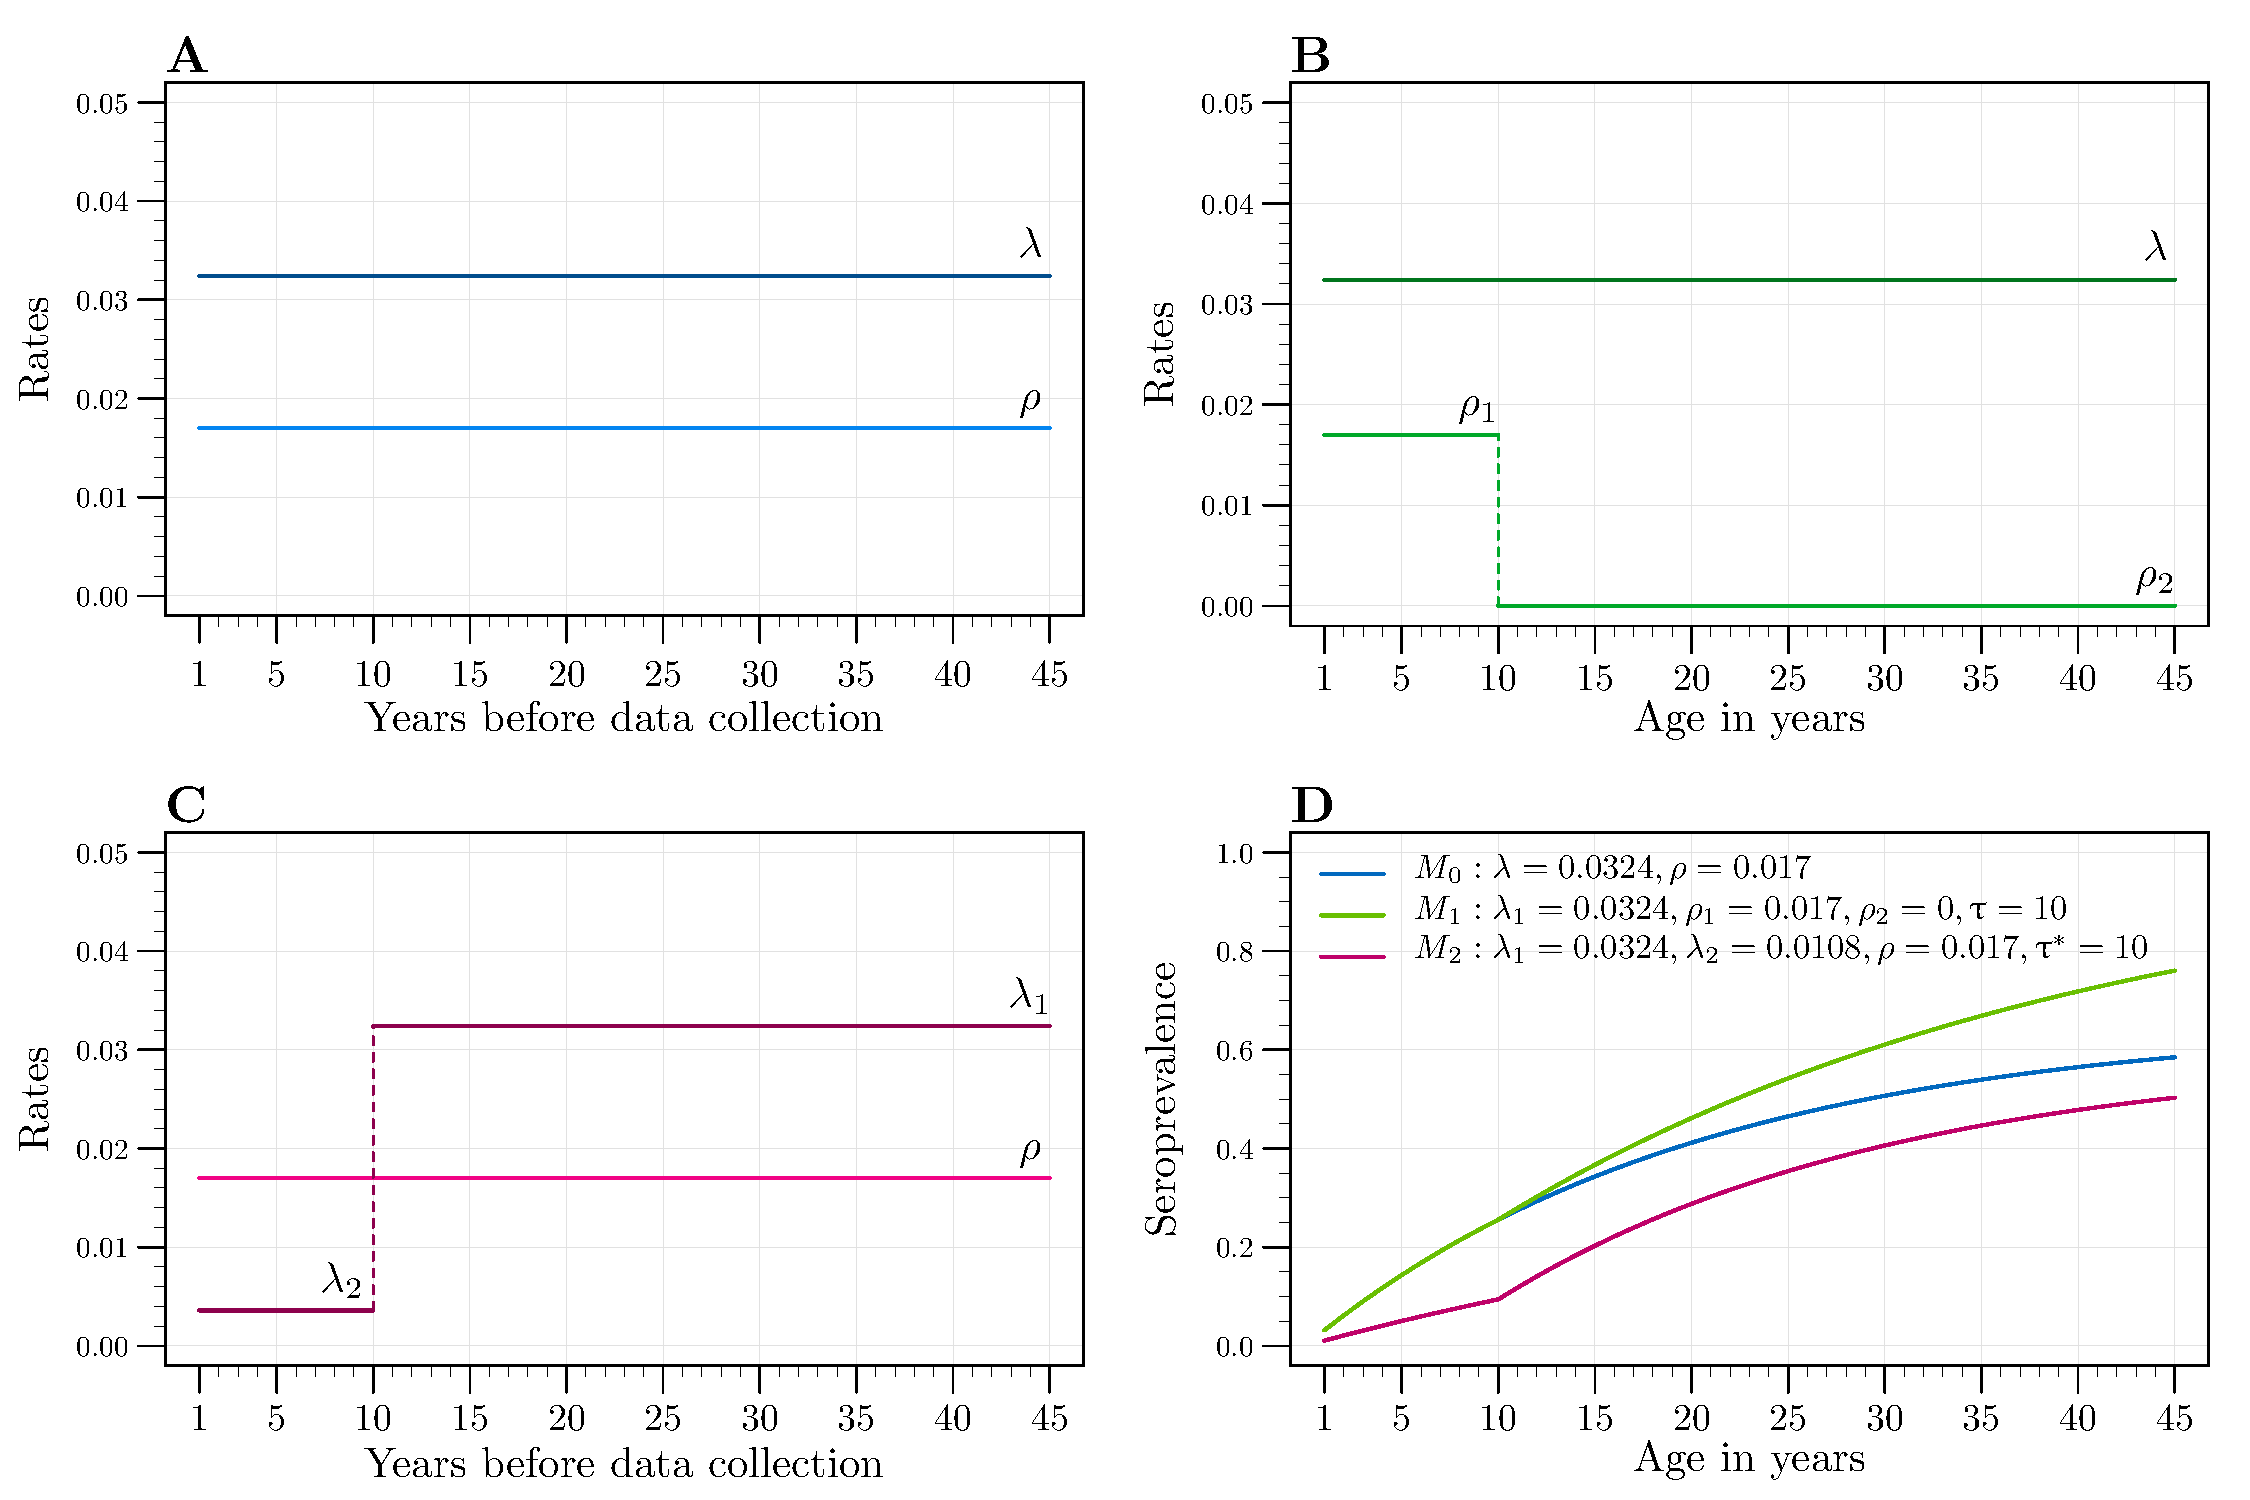
\includegraphics[width=\columnwidth]{images/RCM_structure.pdf}
    \caption[Representation of different possible RCMs]{Graphical representation of the SCR and SRR for each one of the three RCMs described. (\textbf{A}) $\text{M}_0$ with both parameters stable and constant over time; (\textbf{B}) $\text{M}_{1}$ (more specifically model M$_{1,2}$) that assumes SCR to be constant for all ages and SRR to abruptly decrease to a lower value given a change point $\uptau=10$; and (\textbf{C}) $\text{M}_2$ that assumes SCR to change its value after an age cutoff $\uptau^*=10$ while SRR remains constant over time. Plot (\textbf{D}) illustrates the resulting age-dependent seroprevalence calculated for each one of the models.
    % \textcolor{red}{It is worth noting that the SRR biphasic behaviour in $\text{M}_{1,1}$ appears to not reflect a visible effect on the seroprevalence, as shown in curve produced by $\text{M}_2$. It may indicate the smaller influence that SRR has in seroprevalence when compared to SCR -- but an influence nonetheless, as $\pi_t$ visibly increases after $\uptau$, when compared to the curve produced by $\text{M}_0$. -- isto posso tirar devido às novas alterações.}
    }
\label{fig:rcm.models}
\end{figure}


%%%%%%%%%%%%%%%%%%%%%%%%%%%%%%%%
\subsubsection{RCM assuming age-dependent rates to detect heterogeneity in malaria transmission intensity}

%\textbf{aplicar M0}
From a biological point of view, the previous model can be restrictive.
Even in a situation of constant transmission intensity (and thus constant SCR), exposed individuals will eventually develop specific antibodies from an early age, changing SRR over time \cite{cook2011serological}.
%\textbf{because at least SRR can change with age}.
From an epidemiological perspective, considering both rates to be fixed is also limiting.
Model M$_0$ does not account for past actions for control and elimination against the disease that may have occurred, causing SCR to change \cite{cook2010using, sepulveda2015current}.
%\textbf{scr pode mudar devida a intervenções} as modelling serological data under these conditions does not account for acquired immunity over time \cite{cook2011serological} or possible actions for control and elimination against the disease \cite{cook2010using}.
To better represent these two scenarios further mathematical models must be assessed.

In a situation of endemic populations, individuals are expected to gradually develop specific immunity over multiple episodes of infection, throughout their lives \cite{perlmann2002malaria}.
As more individuals become seropositive and remain there due to the constant transmission intensity, over time, less will revert into a seronegative state.
Modelling this effect of acquired immunity should then consider a change in SRR as a function of age.
%that one develops over time can be interpreted as the reduction in SRR over an individual's life, when exposed to stable and constant malaria transmission intensity throughout the hole process.
%The exposure to stable malaria transmission results in a gradual increase of immunological responses, thus individuals that transit to the seropositive state will tend to remain there, adapting to the level of exposure, with consequent antibody waning reduction. 
Mathematically, this age-dependent SRR reduction can be simplified by modelling all individuals with an initial parameter $\rho_1$ that abruptly changes to a different parameter $\rho_2$ after a specific age cutoff $\uptau$.
The change occurs while considering $\lambda_t=\lambda$ (Figure \ref{fig:rcm.models}B).
The age cutoff when such change occurs should vary inversely to the transmission intensity, as individuals exposed to high levels of parasite rate are expected to develop specific immunologic responses earlier in life (standard relation between SCR and expected change in SRR presented in Table \ref{tab:EIR.to.SCR} from Appendices).
%with values between 3 and 5 years in high transmission settings, or values between 15 to 20 years when malaria transmission intensity is lower and requires more time of exposure to adapt.
%for the rest of the individuals' lives 
%This situation is similar to a change due to age-dependent behaviours \cite{}, where mathematically assuming constant SCR, the seroprevalence of an individual aged $t$ years that developed specific immune protection at time $\uptau$ is modelled by the reduction in SRR that follows that instant.
The resulting expected seroprevalence for individuals with age $t$ is explained by model M$_{1,1}$, with formula
%
\begin{equation}
    \label{eq:rcm.reduction.srr}
    \pi_{t | \lambda, \rho_1, \rho_2, \uptau} = \left\{\begin{array}{ll} \frac{\lambda}{\lambda+\rho_{2}}\left(1-e^{-(\lambda+\rho_{2})(t-\uptau)}\right)+\frac{\lambda}{\lambda+\rho_{1}}\left(1-e^{-(\lambda+\rho_{1})\uptau}\right)e^{-(\lambda+\rho_{2})(t-\uptau)}\ , & \text{if $t>\uptau$}\\\\  
    \frac{\lambda}{\lambda+\rho_{1}}\left(1-e^{-(\lambda+\rho_{1})t}\right)\ , & \text{if $t\le\uptau$}\ ,\end{array} \right.
\end{equation}
%
\noindent
where $\lambda \in \rm I\!R_{0}^{+}$ is the SCR constant over time, $\rho_1$ the initial SRR that changes to $\rho_2$ given the cutoff $\uptau$.
Similar to M$_{0}$, this function for seroprevalence increases exponentially.

The derivation of this model is based on a RCM presented by Sepúlveda et al. \cite{sepulveda2015current}.
The original model was used to detect an increase in SCR from children and adolescents to adults, due to age-dependent behaviours.
The model proved useful in populations where the male adults go to work on sites that are malaria transmission hotspots, as opposed to younger individuals who stay within the malaria protected housing regions.
For instance, some mining populations in the Pará state, near the Brazilian Amazonia \cite{cunha2014serologically}.
% An example are some miner populations near the Brazilian Amazonia where the change in SCR estimated occurs between 25 and 30 years old. This increase in transmission intensity coincides with the age of working miners.
%such as populations where the male individuals are sent to work on sites that are malaria transmission hotspots, as opposed to younger individuals who stay within the treated housing regions \cite{}.
Having a similar structure, model M$_{1,1}$ was created considering a change in SRR instead, assuming SCR to be constant throughout the years.
However, to accurately represent the effect of acquired immunity, the model requires the restriction $\rho_1\geq\rho_2$, where $\rho_1 \in  \rm I\!R_{0}^{+}$ (similar to $\rho$ in M$_0$) and $\rho_2 \in [0,\rho_1]$.

In scenarios of endemic malaria with stable SCR, the constant exposure throughout an individual's life results in a gradual development in specific immunity.
This also indicates the whole population will eventually become seropositive, with SRR reduced to nearly zero by the time an individual reaches adulthood \cite{ondigo2014estimation}.
Based on equation (\ref{eq:rcm.reduction.srr}), this scenario can be represented by an abrupt reduction from $\rho_1 \in \rm I\!R_{0}^{+}$, to $\rho_2=0$, after the age cutoff.
With this model (hereafter denoted M$_{1,2}$) one expects that after a certain age, all seropositive individuals will remain so, with resulting expected seroprevalence closer to 1, as age increases.
\\
\\

When considering effective interventions for control of endemic malaria, one expects to infer a noticeable reduction in malaria transmission intensity some time before the sampling \cite{cook2010using}.
Mathematically, this reduction can be represented by admitting SCR as a function of time that changes from $\lambda_1$ to $\lambda_2$, given a cutoff $\uptau^*$, and $\rho_t=\rho$ (Figure \ref{fig:rcm.models}C) \cite{sepulveda2015current}.
%This change can be represented with a similar structure to equation (\ref{eq:rcm.reduction.srr}) by admitting a reduction in transmission rate, modulated by a reduction from $\lambda_1$ to $\lambda_2$, given a change point, $\uptau^*$, some time before sample collection (Figure \ref{fig:rcm.models}C) \cite{sepulveda2015current}.
The resulting seroprevalence in this model (hereafter labelled $\text{M}_{2}$) is described  by
%
\begin{equation}
    \label{eq:rcm.reduction.scr}
    \pi_{t| \lambda_1, \lambda_2, \rho, \uptau^*} = \left\{\begin{array}{ll} \frac{\lambda_{2}}{\lambda_{2}+\rho}\left(1-e^{-(\lambda_{2}+\rho)\uptau^{*}}\right)+\frac{\lambda_{1}}{\lambda_{1}+\rho}\left(1-e^{-(\lambda_{1}+\rho)(t-\uptau^*)}\right)e^{-(\lambda_{2}+\rho)\uptau^{*}}\ , & \text{if $t>\uptau^{*}$} \\\\  \frac{\lambda_{2}}{\lambda_{2}+\rho}\left(1-e^{-(\lambda_{2}+\rho)t} \right)\ , & \text{if $t\le\uptau^{*}$}\ , \end{array}\right.
\end{equation}
%
\noindent
where $\lambda_1$ is the initial SCR parameter that abruptly changes to $\lambda_2$ following the age cutoff $\uptau^*$, and $\rho \in \rm I\!R_{0}^{+}$ is the constant and stable SRR.
%Likewise to the previous models, % seroprevalence is also an increasing function of age, reaching a plateau defined by $\textstyle\frac{\lambda_{1}}{\lambda_{1}+\rho}\left(1-e^{-(\lambda_{1}+\rho)\uptau^*} \right)$ when $t\rightarrow\infty$.
Model M$_2$ is published in Sepúlveda et al. Section 2.3.1 \cite{sepulveda2015current}.
%used to assess changes in malaria transmission due to age-dependent cultural behaviours, such as populations where the male adult individuals are sent to work on sites that are malaria transmission hotspots, as opposed to younger individuals who stay within the treated housing regions \cite{}.
When considering successful interventions, a reduction in malaria transmission intensity is assumed, with corresponding reduction in SCR.
With this change in mind, one can expect a reduction after the cutoff through $\lambda_1\geq\lambda_2$, where $\lambda_1 \in \rm I\!R_{0}^{+}$ and $\lambda_2 \in [0,\lambda_1]$.
%The original model was used to describe changes in malaria intensity due to age-dependent behaviours, in situations where having specific characteristics such as age or gender, might influence the rates of malaria transmission intensity, when compared to other groups of the same population. older individuals may have higher malaria transmission intensity when compared to younger individuals of the same population, due to only being exposed in the working sites.

All variations of the RCMs create slightly different age-dependent seroprevalence curves with influence on the maximum reachable plateaus (Figure \ref{fig:rcm.models}D).
Considering the simpler model M$_{0}$ as reference for the curve analysis, the biphasic behaviour of SRR from M$_{1}$ appears to not reflect a visible effect on the expected seroprevalence as does M$_{2}$ considering variation in SCR.
%\textbf{It may indicate the smaller influence that SRR has in seroprevalence -- but an influence nonetheless. Não vale a pena meter}
Model M$_{0}$ is nested within the remaining RCMs, as is model M$_{1,2}$ in M$_{1,1}$.
This relation means the latter models can be transformed into M$_0$ by imposing certain parametric constrains (Figure \ref{fig:lrt.rcm.models}).
This facilitates model comparisons.
%The RCMs applied to serological data are able to estimate malaria transmission intensity even in low transmission settings \cite{corran2007serology}, applying a stochastic analysis and inferring about exposure over time with data from the cross-sectional study.

\begin{figure}[H]
    \center
    \scalebox{1.05}{\tikzset{every picture/.style={line width=0.75pt}} %set default line width to 0.75pt        

\begin{tikzpicture}[x=0.75pt,y=0.75pt,yscale=-1,xscale=1]
%uncomment if require: \path (0,269.6363525390625); %set diagram left start at 0, and has height of 269.6363525390625

\draw    (100, 80) rectangle (160, 120)   ;
\draw    (300, 80) rectangle (360, 120)   ;
\draw    (200, 178.67) rectangle (260, 218.67)   ;
\draw    (160,100) -- (298,100) ;
\draw [shift={(300,100)}, rotate = 180] [color={rgb, 255:red, 0; green, 0; blue, 0 }  ][line width=0.75]    (10.93,-3.29) .. controls (6.95,-1.4) and (3.31,-0.3) .. (0,0) .. controls (3.31,0.3) and (6.95,1.4) .. (10.93,3.29)   ;

\draw    (260,200) .. controls (309.86,199.95) and (329.96,180.35) .. (330,121.79) ;
\draw [shift={(330,120)}, rotate = 449.65] [color={rgb, 255:red, 0; green, 0; blue, 0 }  ][line width=0.75]    (10.93,-3.29) .. controls (6.95,-1.4) and (3.31,-0.3) .. (0,0) .. controls (3.31,0.3) and (6.95,1.4) .. (10.93,3.29)   ;

\draw    (130,120) .. controls (130.07,179.67) and (149.68,199.87) .. (198.51,200) ;
\draw [shift={(200,200)}, rotate = 539.6800000000001] [color={rgb, 255:red, 0; green, 0; blue, 0 }  ][line width=0.75]    (10.93,-3.29) .. controls (6.95,-1.4) and (3.31,-0.3) .. (0,0) .. controls (3.31,0.3) and (6.95,1.4) .. (10.93,3.29)   ;

\draw    (500, 80) rectangle (560, 120)   ;
\draw    (362,100) -- (500,100) ;

\draw [shift={(360,100)}, rotate = 0] [color={rgb, 255:red, 0; green, 0; blue, 0 }  ][line width=0.75]    (10.93,-3.29) .. controls (6.95,-1.4) and (3.31,-0.3) .. (0,0) .. controls (3.31,0.3) and (6.95,1.4) .. (10.93,3.29)   ;

\draw (130,100) node  [align=left] {M$_{1,1}$};
\draw (330,100) node  [align=left] {M$_{0}$};
\draw (230,200) node  [align=left] {M$_{1,2}$};
\draw (230,80) node [scale=0.9]  {$\rho _{1} =\rho _{2}$};
\draw (110,170) node [scale=0.9]  {$\rho _{2} =0$};
\draw (350,170) node [scale=0.9]  {$\uptau  >T$};
\draw (130,70) node [scale=0.7] [align=left] {$p=4$};
\draw (330,70) node [scale=0.7] [align=left] {$p=2$};
\draw (230,230) node [scale=0.7] [align=left] {$p=3$};
\draw (530,100) node  [align=left] {M$_{2}$};
\draw (440,80) node [scale=0.9]  {$\lambda_{1} =\lambda_{2}$};
\draw (440,120) node [scale=0.9]  {$\uptau^* >T$};
\draw (530,70) node [scale=0.8] [align=left] {$p=4$};


\end{tikzpicture}
}
    \caption[Nested reverse catalytic models]{Schematic representation of the different nested RCMs and the possible parametric restrictions that allow one model to transform into another. M$_{1,2}$ is equivalent to M$_{1,1}$ when $\rho_2\neq0$. M$_{0}$ is equivalent to M$_{1,1}$ when $\rho_1\neq\rho_2$, equivalent to M$_{1,2}$ when $\uptau>T$, or equivalent to M$_{2}$ when $\lambda_1\neq\lambda_2$ or $\uptau^*>T$.
    Values of $p$ indicate the number of parameters in each model.}
    \label{fig:lrt.rcm.models}
\end{figure}



%%%%%%%%%%%%%%%%%%%%%%%%%%%%%%%
% INTRO STATISTICAL INFERENCE %
%%%%%%%%%%%%%%%%%%%%%%%%%%%%%%%
\section{Statistical inference}
\label{sec:inference}

Throughout this thesis, analyses were performed within the frequentist framework.
The method of maximum likelihood was applied to estimate the parameters of the described models.
Two distinct approaches were used when estimating the parameters' confidence intervals.
%The profile likelihood approach used to estimate the RCMs with more than two parameters.
Comparisons between the adjusted models were performed by the Akaike's information Criterion (AIC), the Bayesian information criterion (BIC), the log-likelihood ratio test (for nested models), and the area under curve of the receiving operating characteristic (AUC-ROC).
Finally, goodness-of-fit tests were applied to measure the models' adequacy.

%based on the works of Cressie and Read \cite{cressie1984multinomial}.
%As an alternative, the measures of this thesis could have been approached from a Bayesian perspective, although Bayesian methods were not explored.

%%%%%%%%%%%%%%%%%%%%%%%%%%%%%%%
\subsection{Model estimation}

%%%%%%%%%%%%%%%%%%%%%%%%%%%%%%%
\subsubsection{Maximum likelihood estimation}

Parameter estimation was done by maximising equation (\ref{eq:sampling.distribution}) for the sampling distribution.
%For each independent sample of individuals with age $t$, the \textbf{proportion} of positive or seropositive individuals has a Binomial distribution. The joint density of all the observed values (equation (\ref{eq:sampling})) is the likelihood function, $L\left(\boldsymbol{\pi_t} | \boldsymbol{n_t}; \boldsymbol{m_t}\right)$.
In this method, the maximum likelihood estimates (MLE) are the parameters values that maximise the value of the model's likelihood function based on the observed $m_t$.
Equivalently, one can use the log-likelihood function,
%
%\begin{equation}
%\begin{split}
%\label{eq:mle}
%\log \mathcal{L}(\boldsymbol{\pi_t}|\boldsymbol{n_t},\boldsymbol{m_t}) & =
%\sum_{t=1}^T \log \binom{n_t}{m_t}\pi_t^{\ m_{t}}(1-\pi_t)^{n_t-m_t} \propto \\ 
%& \propto \sum_{t=1}^T n_t\log(1-\pi_t)+m_t\log\left(\frac{\pi_t}{1-\pi_t}\right),
%%\\& \equiv n_t\log [1-\pi_t]+m_t\log \left(\frac{\pi_t}{1-\pi_t}\right).
%\end{split}
%\end{equation}
%\textbf{Esta equação não precisa de ser usada. Se quiser usar tenho de adicionar o índice $k$}\\
%
%\noindent
transforming all products into sums of the likelihood and thus facilitating the maximisation process \cite{williams1994maximum}.
%as its maximisation estimators are easier to calculate through the sum of the log-likelihood \cite{williams1994maximum}.
%\textbf{1) maximizar 3.4), usar log porque tranformo produtos em somas}
MLE are calculated by solving the derivative of the log-transformed equation (\ref{eq:sampling.distribution}) when it is equal to zero.
% \textcolor{red}{ POSSO RETIRAR: The MLE are associated with the regression coefficients $\boldsymbol{\beta}$ that characterise the GLMs and the transitional rates and cutoff parameters in the RCMs, for which the observed sample is more likely to have occurred.}
%Through the properties of the maximum likelihood function,
In theory, the MLE are the realised value of the estimators, being asymptotically unbiased and jointly normal \cite{casella2002statistical}.
%\textbf{ESTIMATORS} (NUNCA \textbf{PREDICTORS})
The unknown parameters for the GLMs and RCM model M$_0$ can be estimated via maximum likelihood estimation, calculating the likelihood of each value that maximises the overall likelihood function.

Maximum likelihood estimates of the regression coefficients in the GLMs were calculated through a software command-defined function.
The method uses the iteratively reweighted least squares (IRLS) for the maximum likelihood estimation, where through a process of weighted iteration, the best linear unbiased estimates $\widehat{\beta}_0,\widehat{\beta}_1,\dots,\widehat{\beta}_k$ are found.
These estimated values are the ones which maximise the likelihood.
% minimise the sum of squared deviations of the observations from their expected values.
% Their respective confidence intervals were obtained by use of the function \texttt{confint()}.
%There are several numerical techniques which can be used to solve the maximum likelihood equations, such as the Newton-Raphson or Expectation-Maximisation algorithm.



%%%%%%%%%%%%%%%%%%%%%%%%%%%%%%%
\subsubsection{Profile likelihood method}

For the particular case of the RCMs M$_1$ (both variations of the model) and M$_2$, with time-dependent parameters $\uptau$ and $\uptau^*$ defined in years, and restricted within the parametric space $\mathbb{N}^{+}$, the use of the simple maximum likelihood estimation is difficult to apply.
% This characteristic makes it difficult to use the simple maximum likelihood estimation.
Knowing that $\uptau$ (although different, for the following description both cutoffs $\uptau$ and $\uptau^*$ will be broadly described using $\uptau$) can be a sequence of positive natural numbers, the profile likelihood method can be used, varying the natural cutoff value in order to estimate the remaining unknown parameters and its respective likelihood.
The estimation is done by the following steps:
(i) the cutoff parameter $\uptau$ is initially fixed at 1;
(ii) the remaining parameters are estimated via maximum likelihood;
(iii) the corresponding log-likelihood function is calculated at these estimates and;
(iv) $\uptau$ is then increased by one unit of time, repeating steps (ii) and (iii) for every increment until it reaches a predefined maximum age value $T$.
In the end, the overall maximum likelihood estimates are the ones associated with the value of $\uptau$ that provide the maximum value of all the log-likelihood estimates calculated.
%but to estimate all unknown parameters $\{\lambda, \rho_1, \rho_2, \uptau\}$, or $\{\lambda_1, \lambda_2, \rho, \uptau^*\}$, when considering an abrupt reduction in SRR (\ref{eq:rcm.reduction.srr}) or SCR (\ref{eq:rcm.reduction.scr}), respectively, a profile likelihood approach can be applied to the data. In this method, parameter $\uptau$ is defined as a sequence of possible values (years) for when the abrupt reduction may occur, starting at $\uptau=1$ and continuously increasing one unit until an agreed maximum limit value. For each update in sequential change in time $\uptau$, the maximum likelihood estimates for all remaining parameters is calculated, as well as the corresponding log-likelihood function. By the end, the overall maximum likelihood estimates are the ones associated with the value of $\uptau$ that returns the maximum value of all the log-likelihood values.
%Though extremely useful, by using exclusively integer values in the change point value, this profile likelihood method may overestimate the exact moment when the change occurs, even when applied to large sample sizes \cite{sepulveda2015current}. To evaluate their significance as more precise models to study seroprevalence, they must be compared with the model assuming stable rates.

%%%%%%%%%%%%%%%%%%%%%%%%
% CONFIDENCE INTERVALS %
%%%%%%%%%%%%%%%%%%%%%%%%
\subsection{Confidence intervals} \label{seq:confint}

The estimation of the confidence interval for the parameters done in the GLMs was based on properties of the maximum likelihood estimators.
%and the Gauss-Markov theorem 
It assumed estimated coefficients $\widehat{{\boldsymbol{\beta}}}$ to be asymptotically normal distributed.
This approach makes use of the most broadly known form of confidence interval estimation, based on the standard error method.
The standard error, $\textstyle\text{se}(\widehat{{\beta}})=\sqrt{V(\widehat{\beta})}$, is defined as the square root of the variance, a measure of variability of the estimate.
% that changes its precision based on the sample size.
Since the $\widehat{\beta}$ are asymptotic normal distributed, the $100(1-\alpha)$\% confidence intervals can be estimated by calculating the lower and upper limits, given the formula
%
\begin{equation}
    \left(\widehat{\beta}\pm \Phi_{\alpha/2} \times \text{se}({\widehat{\beta}})  \right)\ ,
    \label{eq:betas.ci}
\end{equation}
%
\noindent
where $\pm \Phi_{\alpha/2}$ represents the lower and upper quantiles of the standard normal distribution, considering tails of size $\alpha/2$.

While working with the RCMs, in some cases the unknown parameters are expected to present estimated values close to zero.
When in these situations, using the standard deviation method to calculate confidence intervals that close to the parametric space margin may not be the most efficient approach.
%In order to estimate the confidence intervals of these parameters,
For this thesis, the proposed alternative is to make use of the likelihood ratio statistic properties by
%Through this comparison method, a poorly estimated likelihood function 
testing null hypotheses for the acceptance or rejection of each one of the estimated parameters, within a defined critic region.
Considering the case of the RCM M$_0$ and the estimation of the confidence interval of parameter $\lambda$.
Via likelihood ratio, the null and alternative hypothesis in these situations are
%
$$H_0:\lambda=\lambda_0\ \textit{vs.}\ H_1:\lambda \neq \lambda_0\text{\ ,}$$
%
where $\lambda$ is the model's parameter and $\lambda_0$ is a defined estimate.
The likelihood ratio statistics is then based on
%
\begin{equation}
    \text{D}=(-2)\times \left(\Lambda{(\lambda_0,\rho^*)} - \Lambda{(\widehat{\lambda},\widehat{\rho})}\right)\ \overset{a_{\left(\text{H}_0\right)}}{\leadsto}\    \chi_{(1)}^{2}\ ,
\end{equation}
%
\noindent
where $\Lambda{(\lambda_0,\rho^*)}$ is the value of the log-likelihood function under the null hypothesis, with fixed $\lambda_0$ and estimated $\rho^*$, and $\Lambda{(\widehat{\lambda},\widehat{\rho})}$ is the value of the log-likelihood function under the alternative hypothesis with both parameters $\widehat{\lambda}$ and $\widehat{\rho}$ equal to the MLE.
%via profile likelihood.
This test statistic is asymptotically chi-squared distributed under the null hypothesis, with 1 degree of freedom that results from to the difference between the total number of unknown parameters of the models.
The $100(1-\alpha)$\% confidence interval for $\lambda$ is then the range of all possible values of $\lambda$ for which the null hypothesis is not rejected at a given critical region
%equal to or greater than $\text{c}_{\alpha}$.
identified at the level of significance $\alpha$.
This method identifies the confidence intervals as the values for $\lambda$ for which the estimated likelihood ratio test statistic is smaller or equal than the predefined critical value ($\lambda: D\leq \chi^2_{(1)}$).
%This critical region can be \textbf{identified at the 5\% significance} level as the probability of the LRT statistic be equal to or greater than $\text{c}_{\alpha}$.
%The confidence level used was 95\% for a $\alpha=0.05$.
%\textbf{APLICAR NO MODELO M0!!!!}
%Considering the case of the RCM M$_{1,1}$ and parameter $\rho_1$ confidence interval estimation.
%Via likelihood ratio, the null and alternative hypothesis in these situations are 
%$$ H_0:\rho_1=\rho_{1_0}\ \text{vs.}\ H_1:\rho_1 \neq \rho_{1_0}$$
%where $\rho_{1}$ is the model's parameter and $\rho_{1_0}$ is a defined %and instantiated 
%estimate.
%Through the likelihood ratio statistics,
%%
%\begin{equation}
%    \text{LRT}=(-2)\times %\frac{\Lambda_{(\rho_{1_0},\rho_2^*,\lambda^*)}} %{\Lambda_{(\widehat{\rho}_1,\widehat{\rho}_2,\widehat{\lambda})}}\ %\overset{a_{\left(\text{H}_0\right)}}{\leadsto}\    %\chi_{(1)}^{2}
%\end{equation}
%%
%\noindent
%where $\Lambda_{(\rho_{1_0},\rho_2^*,\lambda^*)}$ is the maximum log-likelihood function under the null hypothesis, with fixed $\rho_{1_0}$ and remaining parameters being estimated at each increment of $\uptau$, and $\Lambda_{(\widehat{\rho}_1,\widehat{\rho}_2,\widehat{\lambda})}$ is the estimated maximum log-likelihood function under the alternative hypothesis, with all parameters estimated via profile likelihood.
%This test statistic is chi-squared distributed under the null hypothesis with 1 degree of freedom from to the difference between the total number of parameters in each model.
%\\
%The confidence interval for $\rho_1$ is then the range of all possible values of $\rho_1$ for which the null hypothesis is not rejected at a given critical region $\text{c}_{\alpha}$.
%This critical region can be \textbf{identified at the 5\% significance} level as the probability of the LRT statistic be equal to or greater than $\text{c}_{\alpha}$.
%The confidence level used was 95\% for a $\alpha=0.05$.

%%%%%%%%%%%%%%%%%%%%%%%%%%%%%%%
\subsection{Model comparison}



%%%%%%%%%%%%%%%%%%%%%%%%%%%%%%%
\subsubsection{Information criteria}

The selection of the best fitted models was evaluated using two information criteria: the Akaike's information criterion,
%
\begin{equation}
    \label{eq:aic}
    \text{AIC}=(-2)\times\Lambda_{\text{model}}+2p\ ,
\end{equation}
%
\noindent
and the Bayesian information criterion,
%
\begin{equation}
    \label{eq:bic}
    \text{BIC}=(-2)\times\Lambda_{\text{model}}+p(\log n)\ ,
\end{equation}
%
%Information criteria: AIC (Akaike, 1973) and BIC (Schwarz 1978)
\noindent
%where $\log L(\boldsymbol{\widehat{\beta}}|\boldsymbol{m_t})$ is the maximised value for the log-likelihood function for the model with estimated $\boldsymbol{\widehat{\beta}}$ parameters, and $k$ the number of parameters considered in said model.
where $\Lambda_{\text{model}}$ is the log-likelihood function evaluated at the MLE for the model under consideration, $p$ is the number of parameters, and $n$ is the sample size.
The first term of the criteria reflects the goodness of fit and the second term describes the model's complexity.
The latter adds a penalty for the number of parameters $p$ included. %, penalising overly complex models.
% overfitting and
%When comparing both CRITERIA, BIC is expected to have an increased penalty value.
%since any sample size $n$ above seven individuals will multiply the number of parameters by a higher value than 2.
Under the principle of parsimony, for a set of candidate models the `best' model is the one presenting the smallest values for AIC or BIC. 



%%%%%%%%%%%%%%%%%%%%%%%%%%%%%%%
\subsubsection{Likelihood ratio test}

The Wilks' likelihood ratio test was used to compare the nested RCMs (see Figure \ref{fig:lrt.rcm.models}).
Under a defined null hypothesis for a parametric constrain, this test indicates the more parsimonious model based on the following test statistic
%
\begin{equation}
    \label{eq:lrt}
    \text{LRT} = (-2)\times\left(\Lambda_{\text{H}_0} - \Lambda_{\text{H}_1}\right)\   \overset{a_{\left(\text{H}_0\right)}}{\leadsto}\    \chi_{(\Delta p)}^{2}\ ,
\end{equation}
%
\noindent
where $\Lambda_{\text{H}_0}$ and $\Lambda_{\text{H}_1}$ are the estimated maximum log-likelihood functions of the models that characterise the null and alternative hypothesis.
Under the null hypothesis this test statistic is asymptotically chi-squared distributed, $\chi_{(\Delta p)}^{2}$, where $\Delta p$ degrees of freedom is the difference between the total number of parameters from each one of the compared models (subtracting as $\Delta p = p_{H_{1}}-p_{H_{0}}$).
For a significance level fixed at 0.05, p-values $>0.05$ indicate the model defined by the null hypothesis is statistically better than the model represented by the alternative hypothesis.
%is the log-likelihood estimate for the model assuming constant parameters, with stable values for transmission intensity and antibody waning, $\Lambda_{\text{reduction}}$ the log-likelihood estimate for the model assuming abrupt reduction in either SRR or SCR, and $\chi_{(2)}^{2}$ is a Chi-square distribution with two degrees of freedom resulting from the difference in in the total number of parameters for each one of the respective models, $\lambda$ and $\rho$ in the stable model, and either $\lambda$, $\rho_{1}$, $\rho_{2}$ and $\uptau$ in the model with abrupt reduction in SRR, or $\lambda_1$, $\lambda_2$, $\rho$, and $\uptau^*$ in the model with abrupt reduction in SCR. In case of rejection from the null hypothesis (i.e. p-values under 0.05 for a 5\% significance level) there is statistical evidence to accept a proposed change at an estimated time point.
%For the RCM, log-likelihood ratio test is preferred to the likelihood ratio test to derive confidence intervals rather than the likelihood ratio itself because, provided a sample size



%%%%%%%%%%%%%%%%%%%%%%%%%%%%%%%
\subsubsection{Area under the receiver operating characteristic curve}

The receiver operating characteristic (ROC) curve is a standard technique used to infer about the performance of a model by measuring its predictive outcome accuracy \cite{hosmer2013applied}.
This method explores the trade-off between sensitivity and specificity.
These statistical measures are, respectively, the proportion by which a model correctly predicts a true positive or seropositive individual as a case, and the proportion by which it correctly detects a negative or seronegative individual as a non-case.
Based on sensitivity and specificity, the accuracy of a model depends on how often, and with no wrong predictions, it differentiates between cases and non-cases.

The ROC curve of a model can be plotted for different cutoff points using the sensitivity values (proportion of identified true cases) in function of $1-\text{specificity}$ (proportion of wrongly identified cases).
The resulting area under the ROC curve (AUC), with range from 0 to 1, can be used as an index for a model's accuracy.
AUC values equal to 0 indicate a poorly performing model, misidentifying every single individual of a population sample.
Value of 0.5 predicts that a model is no better than a random guess.
And value of 1 indicates a perfectly accurate model that is able of correctly predict the status of all individuals.
When applied to several models under the same conditions, this measure for predictive accuracy can be used as an index statistics for model comparison.



%%%%%%%%%%%%%%%%%%%%%%%%%
% GOODNESS-OF-FIT TESTS %
%%%%%%%%%%%%%%%%%%%%%%%%%
\section{Goodness-of-fit tests}

To assess the goodness-of-fit of the models, several tests were performed inspecting the agreement between the observed and expected values.
The Hosmer-Lemeshow goodness-of-fit statistic was used to assess the fit of the GLMs \cite{hosmer2013applied}.
This test organises the outcomes in bin-like sub-groups $i=(1,\ldots,g)$, based on percentiles of the estimated probabilities called `deciles of risk groups', and with formula given by
%These sub-groups are usually referred to as `deciles of risk groups'.
%
\begin{equation}
    \label{eq:hosmer.lemeshow}
    C_{HL}^2= \sum_{i=1}^g\frac{(M_{i}-n_{i}\widehat{\pi}_{i})^2}{n_{i}\widehat{\pi}_{i}\left(1-\widehat{\pi}_{i}\right)}\ \overset{a_{\left(\text{H}_0\right)}}{\leadsto}\    \chi_{(g-1)}^{2}\ ,
\end{equation}
%
\noindent
where $M_{i}$ and $n_{i}$ are the number of infected or seropositive individuals and the total number of individuals recorded within each decile of risk group $i$, respectively, $\widehat{\pi}_{i}$ is the prevalence or seroprevalence for individuals in the decile of risk group $i$.
Under the null hypothesis that the model fits the data well, this test statistic is asymptotically chi-squared distributed, $\chi_{(g-1)}^{2}$, with $g-1$ degrees of freedom.
With the intent to create balanced sample sizes across the deciles of risk groups, this test can create a somewhat arbitrarily subdivision of the observations instead of grouping observations by their respective values of variables, possibly lowering the test's power.
%and producing limited results.
%A large p-value in this test may simply indicate the lack of evidence against the null hypothesis and in favour of the alternative hypothesis.

Assuming that more than a single goodness-of-fit test statistic would be applied, the test proposed by Noel Cressie and Timothy Read \cite{cressie1984multinomial} was used, of formula
%
\begin{equation}
    \label{eq:cressie.read}
    \text{CR}^2 = \frac{2}{\delta(\delta+1)} \sum_{i=1}^g M_i \left[ \left(\frac{M_i}{n_i\widehat{\pi}_i}\right)^\delta-1\right]\ \overset{a_{\left(\text{H}_0\right)}}{\leadsto}\    \chi_{(g-1)}^{2}\ ,
\end{equation}
%
%\textbf{COMO É QUE O $p$ É CALCULADO? NUMERO DE GRAUS DE LIBERDADE? NUMERO DE CLASSES?}
\noindent
where $M_i$ and $n_i$ are the number of infected or seropositive individuals and the total number of individuals within a class $i=(1,\dots,g)$, $\widehat{\pi}_i$ is the prevalence or seroprevalence for individuals of that group, $\delta \in \rm I\!R$ is a parameter that depending on its attributed value identifies the different goodness-of-fit tests used, and $g$ is the total number of classes considered.
By varying the values of $\delta$ on the equation, the tests here used are the Pearson's $\chi^2$ ($\delta=1$), the log-likelihood ratio statistic ($\delta=0$), the Freeman-Tukey statistic ($\delta=\textstyle-\frac{1}{2}$), the Neyman modified $\chi^2$ statistic ($\delta=-1$), and the modified log-likelihood ratio statistic ($\delta=-2$).
Under the null hypothesis for no significant difference between the observed and the estimated values, all test statistics are asymptotically chi-squared distributed, $\chi_{(g-1)}^{2}$, with ($g-1$) degrees of freedom.
For a significance level fixed at 0.05, p-values above this limit lead to the non rejection of the hypothesis of equality between the observed frequency distribution and the expected frequencies obtained by the model under testing.
%the recorded infected or seropositive individuals, and the expected numbers 
%
%Under the null hypothesis of equal probabilities, all the proposed tests are asymptotically chi-squared distributed, $\chi_{(\text{p}-1)}^2$, with $\text{p}-1$ degrees of freedom.
%For a significance levels fixed as $5\%$, this hypothesis is rejected for an alternative hypothesis, if the resulting estimated p-value found by use of the $\chi_{\text{p}-1}^2$ expression is greater than or equal to $0.05$.
%Other known alternative tests are then proposed and used, based on the information gathered in the work presented by Noel Cressie and Timothy Read in 1984 \cite{cressie1984multinomial}, where `working rules' are provided to decide which goodness-of-fit test should be used, when considering a Multinomial distribution.
%To test the fitted models, one can infer about the consistency of the calculated probabilities of an individual of age $t$ being positive or seropositive, $\pi_t$, for each model.
%The proposed goodness-of-fit tests are then the most commonly used Pearson's $\chi^2$
%\begin{equation}
%    \label{eq:1.chisquared}
%    X^2=\sum_{t=1}^T \frac{\left(M_t - n_t\pi_t\right)^2}{n_t\pi_t},
%\end{equation}
%\noindent the log-likelihood ratio statistic
%\begin{equation}
%    \label{eq:2.log.LRT.statistic}
%    G^2=2\times\sum_{t=1}^T M_t \log\left(\frac{M_t}{n_t\pi_t}\right),
%\end{equation}
%\noindent the Freeman-Tuckey statistic
%\begin{equation}
%    \label{eq:3.freeman.tuckey}
%    T^2=4\times\sum_{t=1}^T\left[\sqrt{M_t}-\sqrt{n_t\pi_t}\right]^2,
%\end{equation}
%\noindent the Neyman modified $\chi^2$ statistic
%\begin{equation}
%    \label{eq:4.neyman.modified}
%    NM^2=\sum_{t=1}^T \frac{\left(M_t - n_t\pi_t\right)^2}{M_t},
%\end{equation}
%\noindent and the modified log-likelihood ratio statistic
%\begin{equation}
%    \label{eq:5.LRT.modified}
%    GM^2=2\times\sum_{t=1}^T M_t \log\left(\frac{n_t\pi_t}{M_t}\right),
%\end{equation}
%\noindent where for all, $M_t$ is the number of seropositive individuals observed for age $t$, and the multiplication between the total number of individuals with age $t$, $n_t$, with the probability of an individual with that age being seropositive, $\pi_t$, returns the number of expected number of individuals for that age that would be seropositive, based on the values of $\pi_t$ calculated through the different models.
%Under the null hypothesis of equal probabilities, all the proposed tests are asymptotically chi-squared distributed, $\chi_{(\text{p}-1)}^2$, with $\text{p}-1$ degrees of freedom.
%For a significance levels fixed as $5\%$, this hypothesis is rejected for an alternative hypothesis, if the resulting estimated p-value found by use of the $\chi_{\text{p}-1}^2$ expression is greater than or equal to $0.05$.



%%%%%%%%%%%%%%%%%%%%%%%%
% STATISTICAL SOFTWARE %
%%%%%%%%%%%%%%%%%%%%%%%%
\section{Statistical software}

All statistical analyses and inference tests were done in the software R, version 3.4.1.
The command-defined function \texttt{glm()} was applied when calculating the GLMs' regression coeficients
Their respective confidence intervals were obtained by use of the function \texttt{confint()}.
%There are several numerical techniques which can be used to solve the maximum likelihood equations, such as the Newton-Raphson or Expectation-Maximisation algorithm.

\enlargethispage{\baselineskip}
Profile likelihood method to estimate parameters from the RCMs used the \texttt{optim()} function (see the R script used to estimate parameters from RCM M$_{1,1}$ in Appendices \ref{appendix:r.function}).
For each initialised value of $\uptau$, \texttt{optim()} finds the remaining estimates that maximise the likelihood function associated to the model's equation, through consecutive iterations.
The development and analyses of the RCMs done in this thesis helped to develop and test the \emph{SERO-AID} package.
This R package (currently in its final stages of development) was created specifically with the intent to facilitate seroprevalence analyses, allowing the comparisons between different RCMs, such as the M$_0$ or M$_2$.
%%%%%%%%%%%%%%%%%%%%%%%%%%%%%%%%%%%%%%%%
%%%%%   STATISTICAL METHODOLOGY   %%%%%
%%%%%%%%%%%%%%%%%%%%%%%%%%%%%%%%%%%%%%%
\chapter{Statistical methodology}
\label{ch:3.0}

%Mathematical modelling and its analyses have been central to the understanding of infectious diseases in epidemiology. 
The statistical approaches used throughout the thesis are introduced in this chapter.
Section \ref{sec:sampling.distribution} describes the sampling distribution.
All the different sets of stochastic models applied to the data 
%and its statistical principles %used to apply to such data being 
are introduced in Section \ref{sec:models}, and finally, the %basic terminology and fundamental concept
methods used 
%in the field of mathematical modelling of infectious disease dynamics and its transmission are 
for parameter estimation, the approaches used to estimate confidence intervals, models evaluation, and selection, are described in Section \ref{sec:inference}.
%where the principal statistical methods used throughout the thesis for parameter estimation, model evaluation and selection, and inference are explained.
%Since no model can serve all purposes equally well.\textbf{[book - modelling parasite transmission and control]}\\
%In modelling malaria, it is useful to conduct studies that build a broad range of models and that explicitly consider the question of robustness of a model. \textbf{[book - modelling parasite transmission and control]}



%%%%%%%%%%%%%%%%%%%%%%%%%
% SAMPLING DISTRIBUTION %
%%%%%%%%%%%%%%%%%%%%%%%%%
\section{Sampling distribution}
\label{sec:sampling.distribution}

%As previously described in Chapter \ref{ch:2.0}, 
%The data set analysed was created from a cross-sectional study, with the variables registered through single screenings amongst all villages \cite{drakeley2005estimating}.
%The fundamental assumption in order to to apply stochastic methodologies to a cross-sectional data set is to consider individuals' age as proxy for time of exposure.
%By not having follow up data, the key assumption in order to estimate malaria transmission intensity through stochastic methodologies is to  
%This assumption allows to create a measure for historical exposure based on the sequence of the sampled population's age, as one infers older individuals are more likely to have been exposed to malaria parasites \cite{keeling2009mathematical}.
For the data collection in the original study \cite{drakeley2005altitude}, the selected individuals were screened for the presence malaria parasites and three specific \textit{P. falciparum} malarial antigens (MSP1, MSP2, and AMA1).
Each individual was recorded as infected or not infected for malaria, and seropositive or seronegative for the different antigens.
Within each village, the study design placed all sampled individuals in three distinct age groups with defined ranges $[1,5)$, $[5,15)$, and $[15,46)$, each one representing a specific percentage of the %total sampled
recorded population (example of village structure in Table \ref{tab:multinomial.bwambo}).
Under this structured data, the objective of the thesis is then to infer about the number of individuals with status infected/seropositive.

Since the total number of individuals placed within each age group $g=(1,2,3)$ is known, one can assume that the random vector containing the number of
individuals with each combination of characteristics (exact age $i=(I_{g_{min}},\dots,I_{g_{max}})$ and infection or seropositivity status, $j=(0,1)$) follows a Multinomial distribution, where $I_{g_{min}}$ and $I_{g_{max}}$ represent the minimum and the maximum exact ages in age group $g$.
Let $\tilde{X}$ be such vector.
For easiness of reading we shall refer to $\tilde{X}$ as $\tilde{X}_{gij}$ so that track of indexes is kept.
Let $\tilde{x}_{gij}$ be the observed vector and $x_{gij}$ represent the number of individuals in age group $g$, exact age $i$, and status $j$.
The vector $\tilde{x}_{gij}$ is then presented in Table \ref{tab:multinomial.bwambo} with three groups of rows ($g=(1,2,3)$), each with the distribution of the positive and negative cases ($j=(0,1)$) for all the ages within the age group ($i=(I_{g_{min}},\dots,I_{g_{max}})$).
% \textcolor{blue}{the age group has an independent Multinomial distribution, characterised by a sequence of $i=(1,\dots,I_g)$ rows for the ages within each group $g$, and $J=2$ columns, representing the possible outcomes of interest (0 or 1) for the absence or presence of disease infection, or antigens.
% Since the total number of individuals placed within each age group $g=(1,2,3)$ is known, one can assume the age group has an independent Multinomial distribution, characterised by a sequence of $i=(1,\dots,I_g)$ rows for the ages within each group $g$, and $J=2$ columns, representing the possible outcomes of interest (0 or 1) for the absence or presence of disease infection, or antigens.
%, and $J=2$ columns, representing the possible outcomes (0 or 1) for the absence or presence of disease or antigens.
% For a single village, the resulting sampling distribution is then a $I_g \times J$ Multinomial-product for the sequence of the three age groups, given by}
%
\begin{equation}
    \label{eq:multinomial.product}
    \begin{split}
    f(\tilde{x}_{gij} | \tilde{x}_{g\cdot\cdot}, \tilde{\theta}_{gij}) & = \prod_{g=1}^3 \left[ \frac{x_{g\cdot\cdot}!}{\prod_{i=1}^{I_g} \prod_{j=0}^1 x_{gij}!} \prod_{i=1}^{I_g} \prod_{j=0}^1 (\theta_{gij})^{x_{gij}} \right] \\
    & = \prod_{g=1}^3 \left[\frac{x_{g\cdot\cdot}!}{\prod_{i=1}^{I_g} x_{gi0}!x_{gi1}!} \prod_{i=1}^{I_g} (\theta_{gi0})^{x_{gi0}} (\theta_{gi1})^{x_{gi1}} \right],
    \end{split}
\end{equation}
%
\noindent
where $x_{gij}$ is the number of individuals from group $g$, with age $i$, and status outcome $j$, $x_{g\cdot\cdot}$ is the fixed number of sampled individuals contained in the age group $g$, and $\theta_{gij}$ is the joint probability of an individual that belongs to age group $g$ with age $i$, being identified with status $j=(0,1)$.

The following analyses will be focused simply on a single Multinomial distribution from a unspecified age group $g$, with $i=(1,\dots,I)$, as it is simpler to analyse and can be later extended.
%to the sampling distribution.
Under this assumption of a unique age group, $x_{gij}\equiv x_{ij}$, $x_{g\cdot\cdot}\equiv x_{\cdot\cdot}$, and $\theta_{gij}\equiv\theta_{ij}$ .
According to the rule of conditional probability, the joint probability of an individual of age $i$ being identified as having status $j=(0,1)$ can be described as
%
$$\theta_{i1} = \pi_i \gamma_i\text{\ ,}$$ $$\theta_{i0} = (1-\pi_i) \gamma_i\ ,$$
%
\noindent
where $\gamma_i$ is the probability of a sampled individual having age $i$, and $\pi_i$ the probability of an individual of age $i$ being positive for infection or seropositive for the antigens.
The sampling distribution for one village can be then decomposed as follows
%
%\begin{equation}
%    \label{eq:multinomial.distribution}
%    \begin{split}
%    f(\boldsymbol{n_{ij}} | n_{\cdot\cdot}, \boldsymbol{\theta_{ij}}) & = \frac{n_{\cdot\cdot}!}{\prod_{i=1}^In_{i0}!n_{i1}!} \prod_{i=1}^I (\theta_{i0})^{n_{i0}} (\theta_{i1})^{n_{i1}} \\
%    & = \frac{n_{\cdot\cdot}!}{\prod_{i=1}^In_{i0}!n_{i1}!} \prod_{i=1}^I [(1-\pi_i)\gamma_i]^{n_{i0}} \ (\pi_i \gamma_i)^{n_{i1}} \\
%    & = \frac{n_{\cdot\cdot}!}{\prod_{i=1}^In_{i0}!n_{i1}!} \prod_{i=1}^I (1-\pi_i)^{n_{i0}} \ \pi_i^{n_{i1}} \ \gamma_i^{n_{i0}+n_{i1}} \\
%    & = \frac{n_{\cdot\cdot}!}{\prod_{i=1}^In_{i0}!n_{i1}!} \prod_{i=1}^I (1-\pi_i)^{n_{i0}} \ \pi_i^{n_{i1}} \ \gamma_i^{n_{i\cdot}},
%    \end{split}
%\end{equation}
\begin{equation}
    \label{eq:multinomial.distribution}
    \begin{split}
    f(\tilde{x}_{ij} | x_{\cdot\cdot}, \tilde{\theta}_{ij}) & = \frac{x_{\cdot\cdot}!}{\prod_{i=1}^Ix_{i0}!x_{i1}!} \prod_{i=1}^I (\theta_{i0})^{x_{i0}} (\theta_{i1})^{x_{i1}} \\
    & = \frac{x_{\cdot\cdot}!}{\prod_{i=1}^Ix_{i0}!x_{i1}!} \prod_{i=1}^I [(1-\pi_i)\gamma_i]^{x_{i0}} \ (\pi_i \gamma_i)^{x_{i1}} \\
    & = \frac{x_{\cdot\cdot}!}{\prod_{i=1}^Ix_{i0}!x_{i1}!} \prod_{i=1}^I (1-\pi_i)^{x_{i0}} \ \pi_i^{x_{i1}} \ \gamma_i^{x_{i0}+x_{i1}}\ ,
    %& = \frac{n_{\cdot\cdot}!}{\prod_{i=1}^In_{i0}!n_{i1}!} \prod_{i=1}^I (1-\pi_i)^{n_{i0}} \ \pi_i^{n_{i1}} \ \gamma_i^{n_{i\cdot}},
    \end{split}
\end{equation}
%
\noindent
\textcolor{red}{ Corririr para ser legivel: where the resulting sum, an be described as the} marginal frequency of all individuals with age $i$, represented by $x_{i\cdot}$, represented by the expression $x_{i0}+x_{i1}$ .
%Such distribution no longer depends on the vector of probabilities $\boldsymbol{\theta_{ij}}$.
This resulting marginal statistics is characterised by a Multinomial distribution, depending only on the total number of individuals within the group, $x_{\cdot\cdot}$, and parameter $\gamma_i$ .
Since its distribution does not depend on $\pi_i$, $x_{i\cdot}$ is an ancillary statistics for this interest parameter, being a sufficient statistics for $\gamma_i$ \cite{casella2002statistical}.
%This statistics is then an ancillary statistics for the interest parameter $\pi_i$, as its distribution does not depend on the Bernoulli trials for the infection or serological status outcome, being a sufficient statistics for $\gamma_i$ \cite{casella2002statistical}.

%\textbf{quero fazer a inferencia no $\pi$
%Estatística ancilar para o parâmetro de interesse $\pi$}
Under these considerations, one can infer about parameter $\pi_i$ in a way that the Multinomial distribution for the number of positive/seropositive outcomes in age $i$ ($x_{i1}$) is simplified, without losing its information.

\newpage

\begin{equation}
\label{eq:binom}
\begin{split}
f\left(\tilde{x}_{i1} | \tilde{x}_{i\cdot}, \tilde{\gamma}_{i},\tilde{\pi}_{i}\right) &=
\frac{f(\tilde{x}_{i1},\tilde{x}_{i\cdot})} {f(\tilde{x}_{i\cdot} | x_{\cdot\cdot}, \tilde{\gamma}_{i})} \\
& = \frac{\left(\frac{x_{\cdot\cdot}!}{\prod_{i=1}^I (x_{i\cdot}-x_{i1})!x_{i1}!}\right) \prod_{i=1}^I (1-\pi_i)^{x_{i\cdot}-x_{i1}}\ \pi_i^{x_{i1}}\ \gamma_i^{x_{i\cdot}}} {\left(\frac{x_{\cdot\cdot}!}{\prod_{i=1}^I x_{i\cdot}!}\right) \prod_{i=1}^I \gamma_i^{x_{i\cdot}}} \\
& = \prod_{i=1}^I \left(\frac{x_{i\cdot}!}{(x_{i\cdot}-x_{i1})!x_{i1}!}\right) (1-\pi_i)^{x_{i\cdot}-x_{i1}}\ \pi_i^{x_{i1}} \\
& = \prod_{i=1}^I \binom{x_{i\cdot}}{x_{i1}} (1-\pi_i)^{x_{i\cdot}-x_{i1}}\ \pi_i^{x_{i1}}\ .
\end{split}
\end{equation}

\noindent
The frequency of infection/seropositive cases, for each age value $i$ has then a Binomial distribution.
The final sampling distribution for the number of Bernoulli trials for positive or seropositive cases within each age, considering all independent villages studied, $k=(1,\dots,K)$, can be rewritten using the sequence of marginal frequencies for all ages as $t=(1,\dots,T)$, where $T$ is the maximum age recorded for each village, $m_t=x_{i1}$, and $n_t=x_{i_\cdot}$. \textcolor{red}{Manter os índices, em vez de mudar de $i$ para $t$ tenho de meter $t=i$}.
Let $M_{kt}$ represent the number of positive/seropositive individuals amongst the sampled, at village $k$ and with age $t$.
Once again, to facilitate the reading, $\tilde{M}=\{M_{kt}\}$ will be represented as $\tilde{M}_{kt}$ so that track of indexes is kept.
Then, $\tilde{M}_{kt}$ is a vector of size $K\times T$.
Each $M_{kt}$ follows a Binomial distribution with parameters $n_{kt}$ for the total number of sampled individuals with age $t$ from village $k$, and $\pi_{kt}$ for the probability of and individual with age $t$, living at village $k$, being positive or seropositive. 
The resulting sampling distribution formula is then

\begin{equation}
\label{eq:sampling.distribution}
f(\tilde{m}_{kt} | \tilde{n}_{kt}, \tilde{\pi}_{kt}) = \prod_{k=1}^K \prod_{t=1}^T \binom{n_{kt}}{m_{kt}} \pi_{kt}^{\ m_{kt}} (1-\pi_{kt})^{n_{kt} - m_{kt}}\ .
\end{equation}

\noindent
% where $m_{kt}$ and $n_{kt}$ are the number of cases and the total number of sampled individuals with age $t$, recorded at village $k$.
This sampling distribution allows to disregard the initially defined age groups and work solely with the individuals of each age $t$, with prevalence/seroprevalence being assessed through the proportion values for each $t$.
%For the rest of the chapter, equation (\ref{eq:sampling.distribution}) will be referred to considering only a single village, thus removing the product of independent $k$ villages.

\makeatletter
\setlength{\@fptop}{0pt}
\begin{table}[H]
\centering
\caption[Frequency table of infection status in the Bwambo village]{Frequency table of infection status for all sampled individuals from the Bwambo village, from the South Pare transect, ordered by age in years and age group. For each age group $[1,5)$, $[5,15)$, and $[15,46)$, independent and with Multinomial distribution, individuals were selected respecting the $30:30:40$ ratio.
For the village sample size of 396 individuals, each age group $g=(1,2,3)$, has a known $n_{g\cdot\cdot}$, with $n_{1\cdot\cdot}=92$, $n_{2\cdot\cdot}=151$, and $n_{3\cdot\cdot}=153$.
Within each age group $g$, selected individuals were then registered for their age, and screened for presence/absence of malaria parasites.
Each age group, has then a fixed number of frequency columns $J=2$, and specific number of $I_g$ rows, $I_1=4$, $I_2=10$, and $I_3=31$.}
\label{tab:multinomial.bwambo}
\begin{adjustbox}{totalheight=\textheight-5\baselineskip}
\begin{tabular}{ccccc}
\toprule
\multirow{2}{*}{\begin{tabular}[c]{@{}c@{}}Age group,\\$g$\\ \end{tabular}} & \multirow{2}{*}{\begin{tabular}[c]{@{}c@{}}Age, $t$\\in years\\ \end{tabular}} & \multicolumn{2}{c}{Frequency, $j$} & \multirow{2}{*}{$n_{g\cdot\cdot}$}  \\ 
\cmidrule{3-4}
    &     & 0    & 1   &      \\ 
\midrule
1   & 1    & 22   & 1   &      \\
    & 2    & 22   & 0   &      \\
    & 3    & 27   & 1   &      \\
    & 4    & 19   & 0   & 92   \\
\cmidrule{2-5}
2   & 5    & 13   & 0   &      \\
    & 6    & 13   & 2   &      \\
    & 7    & 13   & 1   &      \\
    & 8    & 9    & 0   &      \\
    & 9    & 13   & 1   &      \\
    & 10   & 11   & 0   &      \\
    & 11   & 14   & 1   &      \\
    & 12   & 19   & 1   &      \\
    & 13   & 14   & 1   &      \\
    & 14   & 13   & 1   & 151  \\
\cmidrule{2-5}
3   & 15   & 10   & 1   &      \\
    & 16   & 9    & 0   &      \\
    & 17   & 3    & 0   &      \\
    & 18   & 4    & 0   &      \\
    & 19   & 5    & 0   &      \\
    & 20   & 4    & 0   &      \\
    & 21   & 3    & 0   &      \\
    & 22   & 1    & 0   &      \\
    & 23   & 4    & 0   &      \\
    & 24   & 6    & 0   &      \\
    & 25   & 5    & 0   &      \\
    & 26   & 8    & 0   &      \\
    & 27   & 6    & 0   &      \\
    & 28   & 7    & 0   &      \\
    & 29   & 5    & 0   &      \\
    & 30   & 5    & 1   &      \\
    & 31   & 2    & 0   &      \\
    & 32   & 3    & 0   &      \\
    & 33   & 3    & 0   &      \\
    & 34   & 9    & 0   &      \\
    & 35   & 7    & 0   &      \\
    & 36   & 10   & 0   &      \\
    & 37   & 4    & 0   &      \\
    & 38   & 6    & 0   &      \\
    & 39   & 4    & 0   &      \\
    & 40   & 3    & 1   &      \\
    & 41   & 3    & 1   &      \\
    & 42   & 8    & 0   &      \\
    & 43   & 6    & 0   &      \\
    & 44   & 5    & 0   &      \\
    & 45   & 3    & 0   & 153  \\
\bottomrule
\end{tabular}
\end{adjustbox}
\end{table}
\makeatother


%%%%%%%%%%%%%%%%%%%%%%%%%%%%%%%%
% INTRO TO MATHEMATICAL MODELS %
%%%%%%%%%%%%%%%%%%%%%%%%%%%%%%%%
\section{Statistical models to analyse data}
\label{sec:models}

% Different statistical approaches can be applied when studying malaria transmission intensity.
%Knowing how to apply different methodologies and models is crucial when evaluating or developing projects for public health interventions, or plan for possible infectious disease outbreaks \cite{keeling2009mathematical}.
\textcolor{red}{CORRIGIR: The first set of models used to study prevalence of infection were the generalised linear models (GLMs).
This extension of the linear models was applied to analyse the prevalence of infection amongst sampled individuals.}
From the results, one can identify the principal determinants whose effects may influence transmission intensity.
By studying the characteristics of different well described sites, this approach allows to better understand the patterns causing transmission heterogeneity.
%As an extension to the known linear models, the GLM are equipped to deal with sets of nonGaussian distributions for the response variable, non-constant variance and additivity and independent and identically distributed errors that follow other than the Normal Gaussian distribution with mean 0 and standard deviation $\sigma^{2}$.
The GLMs have been used extensively in epidemiology due to their flexibility \cite{nelder1972glm,andersson2012stochastic}, pairing well with standard measures such as the described parasite rate.
%Though deterministic models are very insightful to study infectious disease spread in large population, they are less useful for small or isolated populations. To this purpose, stochastic models were developed.

After the GLMs, the class of the reverse catalytic models (RCMs) was applied to the serological data.
These specific stochastic models serve as an alternative for the study of infections, and have been used in low transmission settings \cite{corran2007serology}.
Here, the RCMs were used to describe situations of infectious diseases assuming the developed antibodies do not last \textcolor{red}{the entirety -- muito fancy} of an individuals' life.
%such is the case for the malarial antibodies.
%that do not induce  \textbf{long-lasting immunity (aligeirar o jargão!)}, such as malaria.
%Variations of the RCM also allow for the detection of heterogeneity in different epidemiological malaria related scenarios \cite{sepulveda2015current}.
%After the study of a simpler, and largely more used version of the RCMs, some variations are proposed to study the effects of acquired immunity in situations where individuals are exposed to constant levels of disease transmission intensity, or cases of abrupt reduction in malaria transmission due to malaria intervention programs.
Both modelling approaches play an important role in better understanding the different mechanisms of disease transmission rates and its effects on the analysed populations.
%The models were created considering the age-structured sampling distribution, as well as including theoretical relationships among the variables, creating a rational representation of the real world situation in which the data were collected.
%Empirical



%%%%%%%%%%%%%%%%%%%%%%%%%%%%%%%%
\subsection{Generalised linear models to infer about infection determinants}

For a more simplistic theory description, a single unspecified village will be focused.
Thus, the random variable $M_t$ describes the frequency of positively infected individuals with age $t$ in the village, among the sampled.
\textcolor{red}{This Binomial distribution with parameters $n_t$ and $\pi_t$, describing the total number of sampled villagers with age $t$ and the probability of a individual of that age being positive, respectively, is included in the exponential family of distributions. -- simplificar isto}
Under this assumption one can make use of the GLMs.
A GLM is characterised by three distinct components: a random component, a systematic component, and a link function.

For binary outcomes such as the infection status of an individual, the random component identifies the response variables form the each individual.
% for each village (equation (\ref{eq:binom})), or its Multinomial-product (equation (\ref{eq:sampling.distribution})).
%Empirical
%The random component identifies the response variables, assumed to be independent and with distribution included in the exponential family of distributions.This family with standard multiparametric formula for a set of observations $\boldsymbol{X}=(X_1,\dots,X_n)$ given by
%\begin{equation}
%    f(x|\boldsymbol{\theta})=h(x)\ c(\boldsymbol{\theta})\  \exp{\left\{\sum_{i=1}^kw_i(\boldsymbol{\theta})\ t_i(x)\right\}},
%\end{equation}
%\noindent where the base measure $h(x)\geq0$ and $t_1(x),\dots,t_k(t)$ are real-valued functions of the observation $x$ that do not depend on the parameters $\boldsymbol{\theta}$, and $c(\boldsymbol{\theta})\geq0$ and $w_1(\boldsymbol{\theta}),\dots,w_k(\boldsymbol{\theta})$ are real-valued functions of the vector of parameters $\boldsymbol{\theta}$, that do not depend on the observation $x$ \cite{casella2002statistical}.
%When applied to the data set, the random component is characterised by the vector of proportions of the independent observations of positive individuals, $m_t$, in the total number of observations, $n_t$, in each age $t$ in years. Since each response variable has a Binomial distribution with fixed values for the total number of observations across all ages ($t=1,\dots,T$), and probability $\pi_t$ of an individual with age $t$ being identified as positive, its structure defined by the exponential family is then
%\begin{equation}
%    f(\boldsymbol{m_{t}}|\boldsymbol{n_{t}};\boldsymbol{\pi_t})= \prod_{t=1}^T\binom{n_t}{m_t}[1-\pi_t]^{n_t}\ \exp\left\{\sum_{t=1}^T\log\left(\frac{\pi_t}{1-\pi_t}\right)m_t\right\},
    %f(m_t|n_t;\pi_t)=\binom{n_t}{m_t}[1-\pi_t]^{n_t}\ \exp\left\{\log\left(\frac{\pi_t}{1-\pi_t}\right)m_t\right\},
%\end{equation}
%\noindent where $\textstyle h(\boldsymbol{m_t})=\prod_{t=1}^T\binom{n_t}{m_t}$, $\textstyle c(\boldsymbol{\pi_t})=[1-\pi_t]^{n_t}$, $\textstyle w_t(\boldsymbol{\pi_t})=\log\left(\frac{\pi_t}{1-\pi_t}\right)$, and $\textstyle t_t(\boldsymbol{m_t})=\sum_{t=1}^Tm_t$.
%\textstyle\binom{n_t}{m_t%} \geq0$ and $m_t$ are real-valued functions of the observations at each age $t$ that do not depend on $\pi_t$, and $\textstyle[1-\pi_t]^{n_t}\geq0$ and the canonical function, $\textstyle\log\left( \frac{\pi_t}{1-\pi_t}\right)$, are real-valued functions of the probability of seroprevalence at each age, that do not depend on $m_t$.
%
%Via the link function, the linear predictors from the systematic component are linked to the expected value of the response variables that characterise the random component.The given formula of of such link
%The seroprevalence for sampled individuals, in each sampled age, $\pi_t$, can be accessed through regression methods, and since the Binomial distribution for age $t$ is well known and included in the exponential family with formula
%It then becomes possible to make use of the link function, allowing for a degree of non-linearity between the response and the linear predictors. Thus, the expected values of the Binomial response variable, $E(\boldsymbol{m_t})$, is related to the linear predictor via a link function given by
%When talking about regression and modelling a data set, the first and most well known set of model applications would be the linear regression, that develops a linear relationship between a dependent response variable $Y_{i}$ ($i=1,\dots,n$), and a function of linear combinations of $k$ independent variables or predictors $X_{k}$ ($k=1,\dots,K$). This set of models also assumes the random errors as independent and identically distributed, following a Normal Gaussian distribution with mean 0 and standard deviation $\sigma^{2}$ ($\varepsilon_{i} \sim N(0, \sigma^{2})$).
%Assuming the observed values of the infection response for the $n$ individuals, $y_{i}$ $(i=1,\dots,n)$, as having a Bernoulli distribution, the proportion of infected individuals -- response variable $Y_{i}$ -- can be seen as being binomially distributed.\\
%Since this distribution is well known and included in the Exponential Family, it is possible to apply the GLM with the use of link functions, allowing for a degree of non-linearity between the response and the linear predictors that normally would not be possible to study through linear regression. Thus, the expected value of the Binomial response variable, $E(Y_{i})=\mu_{i}$, is related to the linear predictors via link function given by
The systematic component defines a linear combination of the explanatory variables.
Both random and systematic components are related via a link function.
Usually, this function links the expected value of the response variable, $E(M_t)$, with the systematic component of the model.
For a set of binary response variables, rather than directly modelling the dependence of the expected value, the link function explores how the probability of infection, $\pi_t=E(\frac{M_t}{n_t})$, can be described by the observed explanatory variables in the systematic component.
\textcolor{red}{Em termos práticos isto o que faz é um Bernoulli por cada indivíduo}
Given the formula
%
\textcolor{red}{EU AQUI QUERO AS COVARIÁVEIS \textbf{PELO INDIVÍDUO} $i$ E NÃO POR $t$ (Como está atrás! Como tenho de alterar atrás!!!)}
\begin{equation}
    \label{eq:link}
    g(\pi_t)=\beta_0+\beta_1x_{t1}+\dots+\beta_k x_{tk}\ ,
\end{equation}
%
\noindent
where $g(\cdot)$ is the link function that associates both random and systematic components, $\beta_0,\ldots,\beta_k$ are the unknown coefficient parameters, with $\beta_{1},\ldots,\beta_{k}$ being the regression parameters associated with covariates $x_{t1},\ldots,x_{tk}$, respectively, and $\beta_{0}$ representing the \textcolor{red}{efeito médio na ausência de covariáveis} intercept as the overall effect when all the categorical explanatory variables are set to their reference level and the continuous variable is set to zero.
The link function typically transforms the probability of range $[0,1]$ to a value in $(-\infty, +\infty)$.
\textcolor{red}{meter $i$s em vez de $t$!!!!!}

There are different possible link functions.
\textcolor{red}{The functions used throughout the thesis are the logit, probit, cloglog, and are described below described bellow}.
In the case of binary response variables with Binomial distribution, the most used is the logistic link function,
%
\begin{equation}
    \label{eq:logit}
    g(\pi_t)=\log\left(\frac{\pi_t}{1-\pi_t}\right)\ .
\end{equation}
%
\noindent
This transformation is called the canonical link function of the Binomial model, as it is the natural parameter of the Binomial exponential family.
%being the natural parameter of the Binomial exponential family,. 
Since $\frac{\pi_t}{1-\pi_t}$ is the  odds  of an individual with age $t$ being infected, the logit transformation is then the log-odds of this event.
%\noindent that can be rewritten as
%\begin{equation}
%    \pi_t=\frac{e^{g(\pi_t)}}{1+e^{g(\pi_t)}}.
%\end{equation}
%The logistic link function can also provide the odds ratio, making it 
% The logistic link function is used for a wide variety of applications such as epidemiological and biomedical fields.
Other known link functions used are the probit link function,
%
\begin{equation}
    \label{eq:probit}
    g(\pi_t)=\Phi^{-1}(\pi_t)\ ,
\end{equation}
%
\noindent
that uses an inverse normal link function, and the complementary log-log link function
%
\begin{equation}
    \label{eq:cloglog}
    g(\pi_t)=\log[-\log(1-\pi_t)]\ .
\end{equation}

%\noindent
%which is the inverse .
The GLMs take into consideration the variables described in Chapter \ref{ch:2.0}, as well as potential relationships amongst them, better recreating a rational representation of the real world situation in which the data were collected.



%%%%%%%%%%%%%%%%%%%%%%%%%%%%%%%%
\subsection{Specific models for estimating malaria transmission intensity}

When modelling serological data, individuals are generally assumed to be born seronegative\textcolor{red}{, without protective immunity and susceptible to potential malaria infections -- isto pode ir c'o caralho}.
Upon exposure to malaria parasites, individuals might become seropositive by producing antibodies to deal with the infection.
Since malaria does not induce long lasting immunity, seropositive individuals can later revert into a seronegative state in the absence of continued exposure and recurrent infections.
This process of sequential change between two serological states can be described by the reverse catalytic models (RCMs).
The RCMs are mathematically formulated as a two state Markov Chain, where individuals transit between the seronegative and seropositive states (Figure \ref{fig:M0}).
The transitions from one state to the other occur at specific age-dependent rates that allow to quantify the levels of parasite exposure and malaria transmission intensity \cite{muench1959catalytic}.

\begin{figure}[ht!]
    \center
    \scalebox{1.25}{\begin{tikzpicture}[x=0.75pt,y=0.75pt,yscale=-1,xscale=1]
%uncomment if require: \path (0,300); %set diagram left start at 0, and has height of 300

\draw    (160, 120) rectangle (220, 160)   ;
\draw    (280, 120) rectangle (340, 160)   ;
\draw    (220,130) -- (280,130) ;
\draw [shift={(280,130)}, rotate = 180] [color={rgb, 255:red, 0; green, 0; blue, 0 }  ]   (0,0) .. controls (3.31,-0.3) and (6.95,-1.4) .. (10.93,-3.29)(0,0) .. controls (3.31,0.3) and (6.95,1.4) .. (10.93,3.29)   ;

\draw    (220,150) -- (280,150) ;

\draw [shift={(220,150)}, rotate = 0] [color={rgb, 255:red, 0; green, 0; blue, 0 }  ]   (0,0) .. controls (3.31,-0.3) and (6.95,-1.4) .. (10.93,-3.29)(0,0) .. controls (3.31,0.3) and (6.95,1.4) .. (10.93,3.29)   ;

\draw (190,140) node  [align=left] {S$^{-}$};
\draw (310,140) node  [align=left] {S$^{+}$};
\draw (250,120) node  [align=left] {$\lambda_t$};
\draw (250,160) node  [align=left] {$\rho_t$};
\end{tikzpicture}}
    \caption[Reverse catalytic model with constant transition parameters]{Schematic representation of the reverse catalytic model, where individuals transit between seronegative ($\text{S}^-$) and seropositive ($\text{S}^+$) states with age-dependent rates $\lambda_t$ (seroconversion rate) and $\rho_t$ (seroreversion rate).}
    \label{fig:M0}
\end{figure}

The seroconversion rate (SCR or $\lambda_t$) is the annual average rate by which individuals with age $t$ change from seronegative to seropositive, upon malaria infection.
This rate is directly related to transmission intensity and has shown to correlate well with popular epidemiological measures of malaria transmission such as parasite and entomological inoculation rate \cite{corran2007serology, drakeley2005estimating, bodker2003relationship}.
Seroreversion rate (SRR or $\rho_t$) is the annual average rate by which seropositive individuals with age $t$ return to the seronegative state due to antibody decay.
This rate can be influenced by individual characteristics such as age or genetics \cite{corran2007serology}, and be used to predict how many seropositive individuals are expected to remain after complete interruption of transmission \cite{corran2007serology}.
%\\ in the absence of \\
%RECURRENT
%prolonged
%infection 
%The use of these models have the Markov property of lack of memory in a stochastic process, where for time $t$, the probability of transition from one state to another does not depend on previous transitions.This allows for the assumption of a probabilistic restart every time an individual transits from one state to the other.The probability of an individual with age $t$ being at one of the serological states is then defined by a probability matrix
%
%\begin{equation}
%    P(t)=[p_{i|j}(t)], \quad i,j=0,1 ,
%\end{equation}
%
%\noindent where $p_{i|j}(t)$ is the conditional probability of an individual with age $t$ being in state $i$ given he started the process in the state $j$. Making use of these probabilities, the transitional rates can be defined through the transition rate matrix,
%\begin{gather}
%    R = \begin{bmatrix} -\lambda    & \lambda \\ 
%                        \rho        & -\rho \end{bmatrix}
%\end{gather}
%\noindent where $\lambda$ and $\rho$, respectively representing the SCR and SRR, are the transition parameters from one state to the other. The presented negative values for the parameters in the matrix are simply to assure the sum of each line is equal to zero. 

When using RCMs to estimate malaria transmission intensity, one should assume the lower age limit to be $t=1$ year old.
While all individuals are usually assumed to be born seronegative ($\pi_0=0$), when dealing with responses to malaria parasites, the new born's immune system may be influenced by the presence of inherited maternal antibodies.
These antibodies eventually wane over the first months of the newborn's life.
By removing the first year from the analyses, the influence of the maternal antibodies in the model's estimates is expected to be reduced.
% that \textcolor{red}{outsourced} influence is expected to be reduced.
% \textcolor{red}{reduced the maternal antibodies in the analysis.}


%%%%%%%%%%%%%%%%%%%%%%%%%%%%%%%%
\subsubsection{Malaria under stable transmission intensity}

\textcolor{red}{TENHO DE METER QUE $t>0$}
%Following the previous definitions, a RCM that assumes the transitional rates as constant per unit of time $t$ can be created \cite{muench1959catalytic}.
The simplest RCM assumes both SCR and SRR to be constant over time: $\lambda_t =\lambda$ and $\rho_t = \rho$ (Figure \ref{fig:rcm.models}A).
In this situation, all individuals experience equal risk of exposure at all times.
The expected seroprevalence of individuals with age $t$ explained by this model, henceforward denoted M$_0$, is given by
%
\begin{equation}
    \label{eq:M0}
    \pi_{t|\lambda, \rho}=\frac{\lambda}{\lambda+\rho}\left(1-e^{-(\lambda+\rho)t}\right)\ ,
\end{equation}
%
\noindent
where $\lambda \in \rm I\!R_{0}^{+}$ and $\rho \in \rm I\!R_{0}^{+}$.
Both transition rates are expected to be positive, although the possibilities for $\lambda=0$ and $\rho=0$ are included to allow for some particular cases.
A null SCR value can happen if, by any change, a population has experienced transmission interruption.
In that situation any model will predict seroprevalence equal to zero.
A null SRR indicates that all individuals who are exposed and become positively infected \textbf{(SEROPOSITIVE)} will remain so throughout their remaining life.
Model M$_0$ is an increasing function of age that tends exponentially to a plateau given by $\textstyle\frac{\lambda}{\lambda+\rho}$, when $t\rightarrow\infty$.
The derivation of the equation can be found in Section \ref{appendix:M0.derivation} from Appendices.

While not common to use this model in situations of null SCR, it is worth mention that there are situations where SRR can become a rare event.
When this happens, by considering $\rho\rightarrow0$ the model can be rewritten as a traditional complementary log-log model, with resulting formula
%
\begin{equation}
    \label{eq:rcm.cloglog}
    \log[-\log(1-\pi_t)]=\log\lambda+\log t\ .
\end{equation}
%
\noindent
However, this \textcolor{red}{cloglog -- não defini a abreviatura} model is not usually used in malaria research, but has been used to study scenarios where a unique exposure to the disease develops immunisation with resulting permanent seropositive state \cite{hens2012modeling}.

\begin{figure}[th!]
    \center
    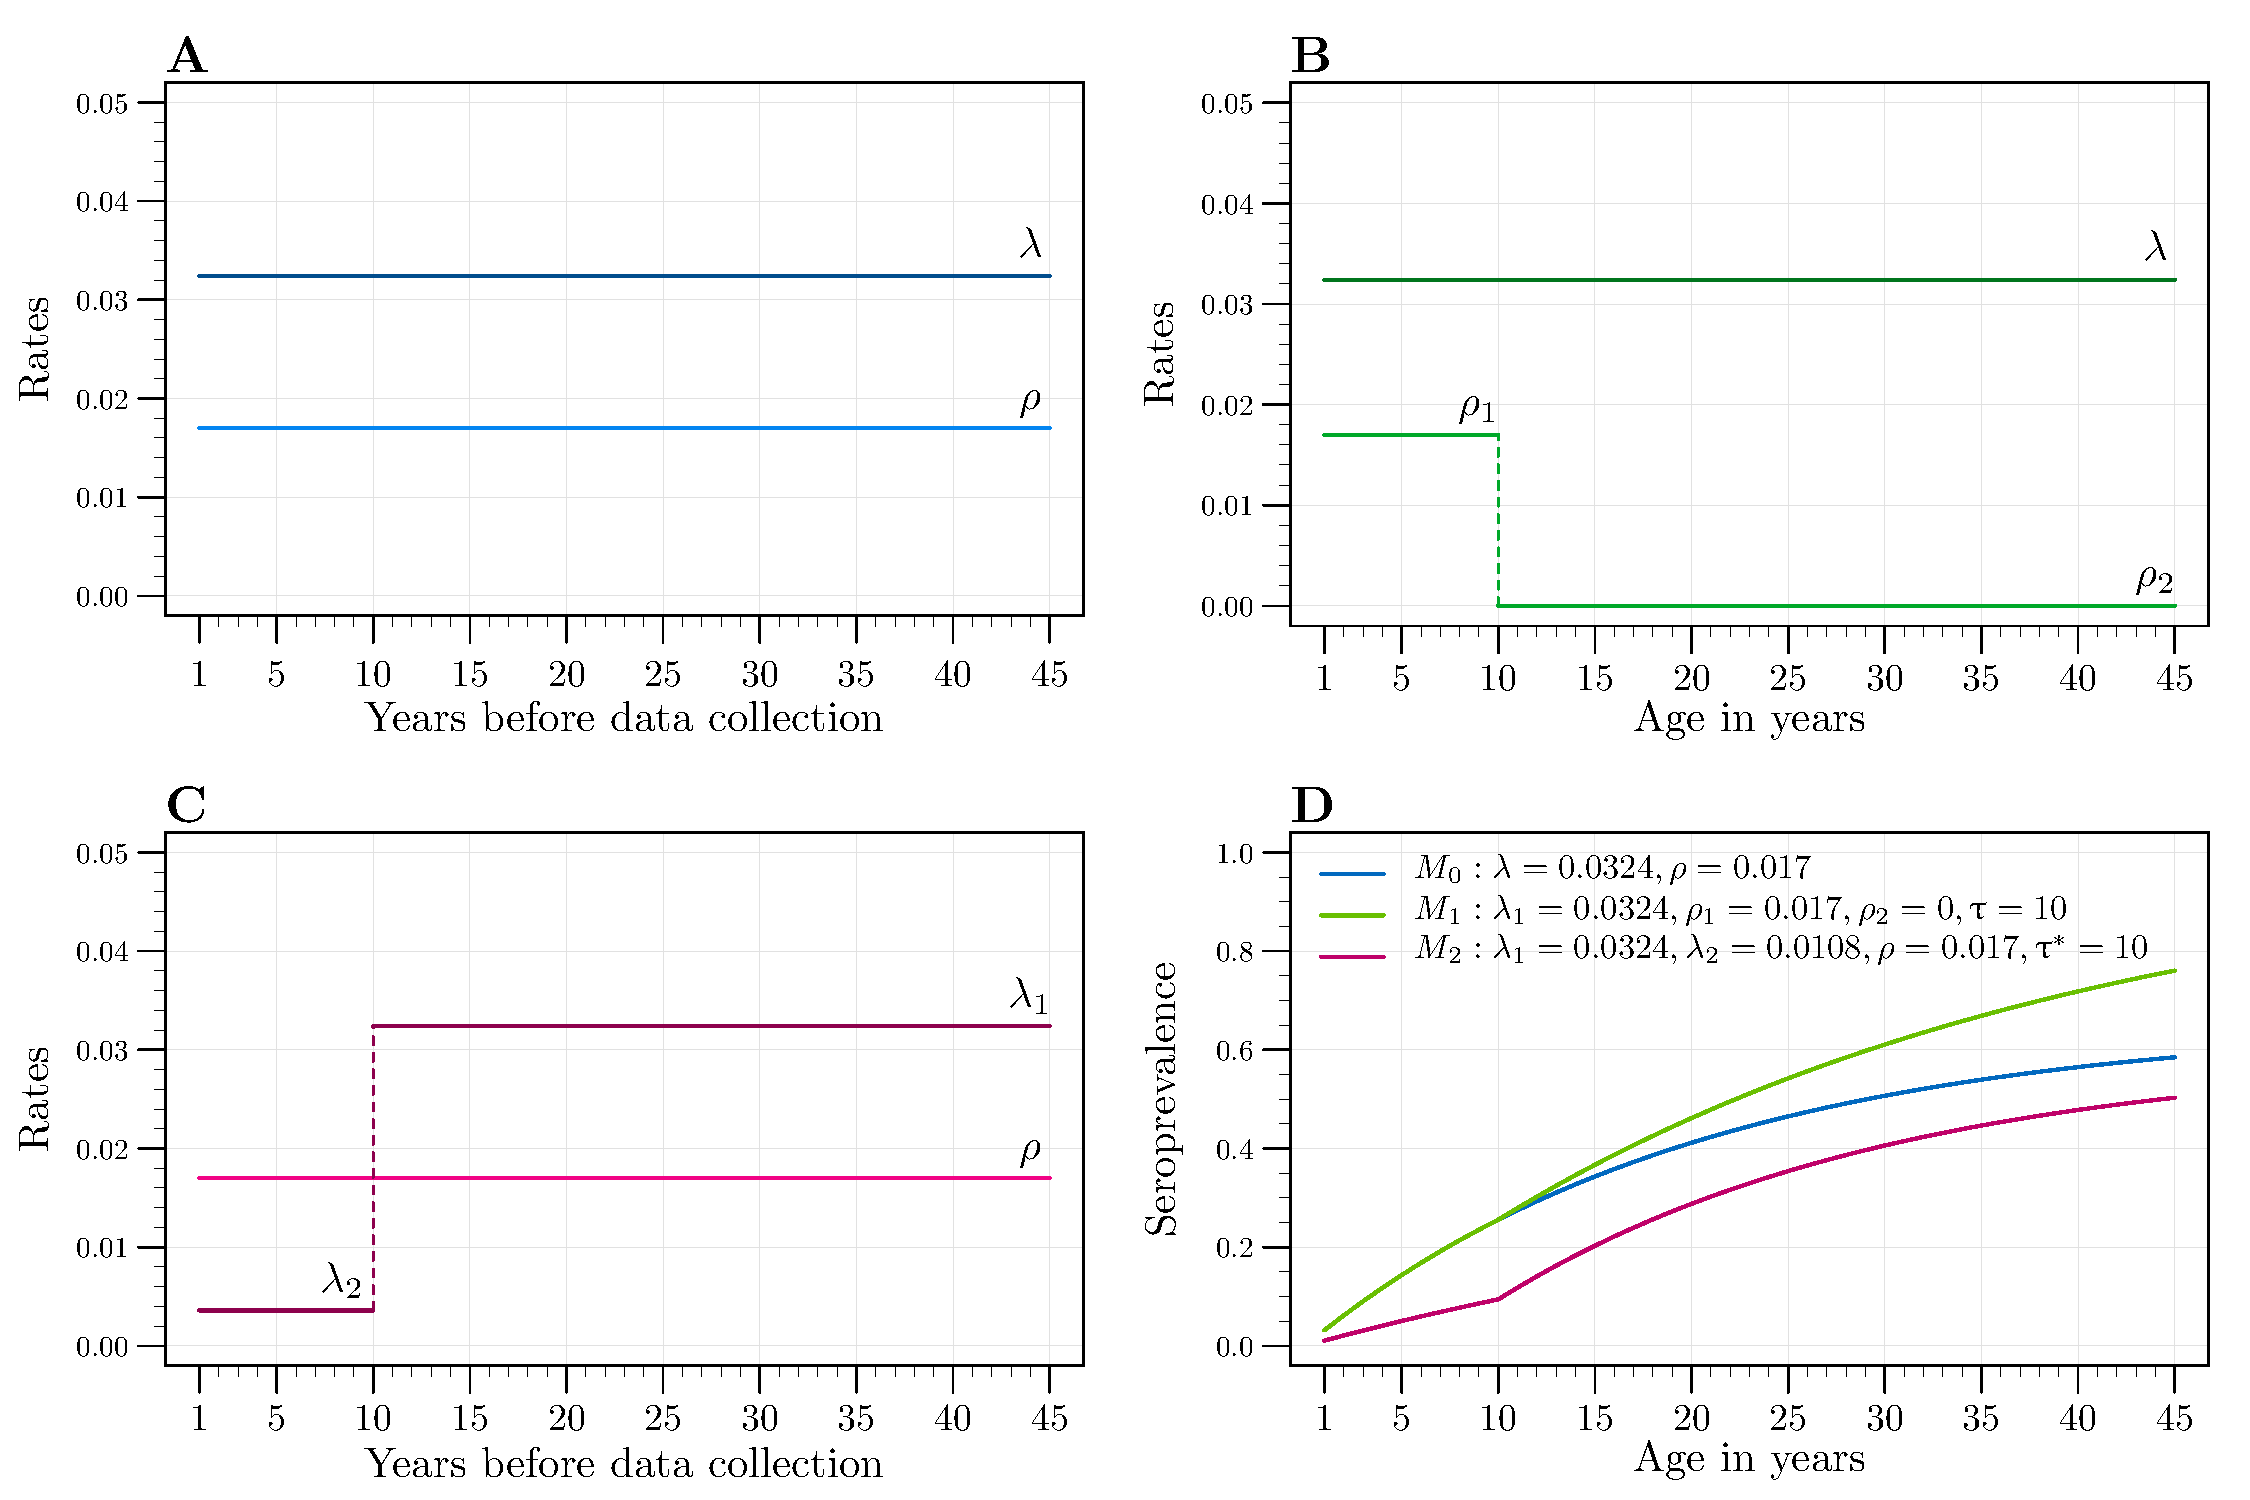
\includegraphics[width=\columnwidth]{images/RCM_structure.pdf}
    \caption[Reverse catalytic models]{Graphical representation of the SCR and SRR for each one of the three RCM described. (\textbf{A}) $\text{M}_0$ with both parameters stable and constant over time; (\textbf{B}) $\text{M}_{1,1}$ that assumes SCR to be constant for all ages and SRR to abruptly decrease to a lower value given an age cutoff $\uptau=10$; and (\textbf{C}) $\text{M}_2$ that assumes SCR to reduce to a lower value, after a change point $\uptau^*=10$. Plot (\textbf{D}) illustrates the resulting age-dependent seroprevalence calculated for each one of the models. \textcolor{red}{It is worth noting that the SRR biphasic behaviour in $\text{M}_{1,1}$ appears to not reflect a visible effect on the seroprevalence, as shown in curve produced by $\text{M}_2$. It may indicate the smaller influence that SRR has in seroprevalence when compared to SCR -- but an influence nonetheless, as $\pi_t$ visibly increases after $\uptau$, when compared to the curve produced by $\text{M}_0$. -- isto posso tirar devido às novas alterações.}}
\label{fig:rcm.models}
\end{figure}


%%%%%%%%%%%%%%%%%%%%%%%%%%%%%%%%
\subsubsection{RCM assuming age-dependent rates to detect heterogeneity in malaria transmission intensity}

%\textbf{aplicar M0}
From a biological point of view, the previous model can be restrictive.
Even in a situation of constant transmission intensity (and thus constant SCR), exposed individuals will eventually develop specific antibodies from an early age, changing SRR over time \cite{cook2011serological}.
%\textbf{because at least SRR can change with age}.
From an epidemiological perspective, considering both rates to be fixed is also limiting.
Model M$_0$ does not account for past actions for control and elimination against the disease that may have occurred, causing SCR to change \cite{cook2010using, sepulveda2015current}.
%\textbf{scr pode mudar devida a intervenções} as modelling serological data under these conditions does not account for acquired immunity over time \cite{cook2011serological} or possible actions for control and elimination against the disease \cite{cook2010using}.
To better represent these two scenarios further mathematical models must be assessed.

In a situation of endemic populations, individuals are expected to gradually develop specific immunity over multiple episodes of infection, throughout their lives \cite{perlmann2002malaria}.
As more individuals become seropositive and remain there due to the constant transmission intensity, over time, less will revert to a seronegative state.
Modelling this effect of acquired immunity should then consider a change in SRR as a function of age.
%that one develops over time can be interpreted as the reduction in SRR over an individual's life, when exposed to stable and constant malaria transmission intensity throughout the hole process.
%The exposure to stable malaria transmission results in a gradual increase of immunological responses, thus individuals that transit to the seropositive state will tend to remain there, adapting to the level of exposure, with consequent antibody waning reduction. 
Mathematically, this \textcolor{red}{variation variação do quê?} can be simplified by modelling all individuals with an initial parameter $\rho_1$ that abruptly changes to a different parameter $\rho_2$ after a specific age cutoff $\uptau$.
The change occur while considering $\lambda_t=\lambda$ (Figure \ref{fig:rcm.models}B).
The age cutoff when such change occurs should vary inversely to the transmission intensity, as individuals that are exposed to high levels of parasite rate are expected to develop specific immunologic responses earlier in life (standard relation between SCR and change in SRR presented in Table \ref{tab:EIR.to.SCR} from Appendices).
%with values between 3 and 5 years in high transmission settings, or values between 15 to 20 years when malaria transmission intensity is lower and requires more time of exposure to adapt.
%for the rest of the individuals' lives 
%This situation is similar to a change due to age-dependent behaviours \cite{}, where mathematically assuming constant SCR, the seroprevalence of an individual aged $t$ years that developed specific immune protection at time $\uptau$ is modelled by the reduction in SRR that follows that instant.
The resulting expected seroprevalence for individuals with age $t$ is explained by model M$_{1,1}$, with formula
%
\begin{equation}
    \label{eq:rcm.reduction.srr}
    \pi_{t | \lambda, \rho_1, \rho_2, \uptau} = \left\{\begin{array}{ll} \frac{\lambda}{\lambda+\rho_{1}}\left(1-e^{-(\lambda+\rho_{1})\uptau}\right)+\frac{\lambda}{\lambda+\rho_{2}}\left(1-e^{-(\lambda+\rho_{2})(t-\uptau)}\right)e^{-(\lambda+\rho_{1})\uptau}\ , & \text{if $t>\uptau$}\\\\  
    \frac{\lambda}{\lambda+\rho_{1}}\left(1-e^{-(\lambda+\rho_{1})t}\right)\ , & \text{if $t\le\uptau$}\ ,\end{array} \right.
\end{equation}
%
\noindent
where $\lambda \in \rm I\!R_{0}^{+}$ is the SCR constant over time, $\rho_1$ the initial SRR that changes to $\rho_2$ given the cutoff $\uptau$.
Similar to M$_{0}$, this function for seroprevalence increases exponentially.

The derivation of this model is based on a RCM presented by Sepúlveda et al. \cite{sepulveda2015current}.
The original model was used to detect an increase in SCR from children and adolescents to adults, due to age-dependent behaviours.
The model proved useful in populations where the male adults go to work on sites that are malaria transmission hotspots, as opposed to younger individuals who stay within the malaria protected housing regions.
\textcolor{red}{Are example -- isto é inglês ali do Pub} some mining populations in the Pará state, near the Brazilian Amazonia \cite{cunha2014serologically}.
% An example are some miner populations near the Brazilian Amazonia where the change in SCR estimated occurs between 25 and 30 years old. This increase in transmission intensity coincides with the age of working miners.
%such as populations where the male individuals are sent to work on sites that are malaria transmission hotspots, as opposed to younger individuals who stay within the treated housing regions \cite{}.
Having a similar structure, model M$_{1,1}$ was created considering a change in SRR instead, assuming SCR to be constant throughout the years.
However, to accurately represent the effect of acquired immunity, the model requires the restriction $\rho_1\geq\rho_2$, where $\rho_1 \in  \rm I\!R_{0}^{+}$ (similar to $\rho$ in M$_0$) and $\rho_2 \in [0,\rho_1]$.

In scenarios of endemic malaria with stable SCR, the constant exposure throughout an individual's life results in a gradual development in specific immunity.
This also indicates the whole population will eventually become seropositive, with SRR reduced to nearly zero by the time an individual reaches adulthood \cite{ondigo2014estimation}.
Based on equation (\ref{eq:rcm.reduction.srr}), this scenario can be represented by an abrupt reduction from $\rho_1 \in \rm I\!R_{0}^{+}$, to $\rho_2=0$, after the age cutoff.
With this model (hereafter denoted M$_{1,2}$) one expects that after a certain age, all seropositive individuals will remain so, with resulting expected seroprevalence closer to 1, as age \textcolor{red}{increases/advances}.
\\
\\

When considering effective interventions for control of endemic malaria, one expects to infer a noticeable reduction in malaria transmission intensity some time before the sampling \cite{cook2010using}.
Mathematically, this reduction can be represented by admitting SCR as a function of time that changes from $\lambda_1$ to $\lambda_2$, given a cutoff $\uptau^*$, and $\rho_t=\rho$ (Figure \ref{fig:rcm.models}C) \cite{sepulveda2015current}.
%This change can be represented with a similar structure to equation (\ref{eq:rcm.reduction.srr}) by admitting a reduction in transmission rate, modulated by a reduction from $\lambda_1$ to $\lambda_2$, given a change point, $\uptau^*$, some time before sample collection (Figure \ref{fig:rcm.models}C) \cite{sepulveda2015current}.
The resulting seroprevalence in this model (hereafter labelled $\text{M}_{2}$) is described  by
%
\begin{equation}
    \label{eq:rcm.reduction.scr}
    \pi_{t| \lambda_1, \lambda_2, \rho, \uptau^*} = \left\{\begin{array}{ll} \frac{\lambda_{2}}{\lambda_{2}+\rho}\left(1-e^{-(\lambda_{2}+\rho)\uptau^{*}}\right)+\frac{\lambda_{1}}{\lambda_{1}+\rho}\left(1-e^{-(\lambda_{1}+\rho)(t-\uptau^*)}\right)e^{-(\lambda_{2}+\rho)\uptau^{*}}\ , & \text{if $t>\uptau^{*}$} \\\\  \frac{\lambda_{2}}{\lambda_{2}+\rho}\left(1-e^{-(\lambda_{2}+\rho)t} \right)\ , & \text{if $t\le\uptau^{*}$}\ , \end{array}\right.
\end{equation}
%
\noindent
where $\lambda_1$ is the initial SCR parameter that abruptly changes to $\lambda_2$ following the age cutoff $\uptau^*$, and $\rho \in \rm I\!R_{0}^{+}$ is the constant and stable SRR.
%Likewise to the previous models, % seroprevalence is also an increasing function of age, reaching a plateau defined by $\textstyle\frac{\lambda_{1}}{\lambda_{1}+\rho}\left(1-e^{-(\lambda_{1}+\rho)\uptau^*} \right)$ when $t\rightarrow\infty$.
Model M$_2$ is published in Sepúlveda et al. Section 2.3.1 \cite{sepulveda2015current}.
%used to assess changes in malaria transmission due to age-dependent cultural behaviours, such as populations where the male adult individuals are sent to work on sites that are malaria transmission hotspots, as opposed to younger individuals who stay within the treated housing regions \cite{}.
When considering successful interventions, a reduction in malaria transmission intensity is assumed, with corresponding reduction in SCR.
With this change in mind, one can expect a reduction after the cutoff through $\lambda_1\geq\lambda_2$, where $\lambda_1 \in \rm I\!R_{0}^{+}$ and $\lambda_2 \in [0,\lambda_1]$.
%The original model was used to describe changes in malaria intensity due to age-dependent behaviours, in situations where having specific characteristics such as age or gender, might influence the rates of malaria transmission intensity, when compared to other groups of the same population. older individuals may have higher malaria transmission intensity when compared to younger individuals of the same population, due to only being exposed in the working sites.

All variations of the RCMs create slightly different age-dependent seroprevalence curves with influence on the maximum reachable plateaus (Figure \ref{fig:rcm.models}D).
Considering the simpler model M$_{0}$ as reference for the curve analysis, the biphasic behaviour of SRR from M$_{1}$ appears to not reflect a visible effect on the expected seroprevalence as does M$_{2}$ considering variation in SCR.
%\textbf{It may indicate the smaller influence that SRR has in seroprevalence -- but an influence nonetheless. Não vale a pena meter}
Model M$_{0}$ is nested within the remaining RCMs, as is model M$_{1,2}$ in M$_{1,1}$.
This relation means the latter models can be transformed into M$_0$ by imposing certain parametric constrains (Figure \ref{fig:lrt.rcm.models}).
This facilitates model comparisons.
%The RCMs applied to serological data are able to estimate malaria transmission intensity even in low transmission settings \cite{corran2007serology}, applying a stochastic analysis and inferring about exposure over time with data from the cross-sectional study.

\begin{figure}[H]
    \center
    \scalebox{1.05}{\tikzset{every picture/.style={line width=0.75pt}} %set default line width to 0.75pt        

\begin{tikzpicture}[x=0.75pt,y=0.75pt,yscale=-1,xscale=1]
%uncomment if require: \path (0,269.6363525390625); %set diagram left start at 0, and has height of 269.6363525390625

\draw    (100, 80) rectangle (160, 120)   ;
\draw    (300, 80) rectangle (360, 120)   ;
\draw    (200, 178.67) rectangle (260, 218.67)   ;
\draw    (160,100) -- (298,100) ;
\draw [shift={(300,100)}, rotate = 180] [color={rgb, 255:red, 0; green, 0; blue, 0 }  ][line width=0.75]    (10.93,-3.29) .. controls (6.95,-1.4) and (3.31,-0.3) .. (0,0) .. controls (3.31,0.3) and (6.95,1.4) .. (10.93,3.29)   ;

\draw    (260,200) .. controls (309.86,199.95) and (329.96,180.35) .. (330,121.79) ;
\draw [shift={(330,120)}, rotate = 449.65] [color={rgb, 255:red, 0; green, 0; blue, 0 }  ][line width=0.75]    (10.93,-3.29) .. controls (6.95,-1.4) and (3.31,-0.3) .. (0,0) .. controls (3.31,0.3) and (6.95,1.4) .. (10.93,3.29)   ;

\draw    (130,120) .. controls (130.07,179.67) and (149.68,199.87) .. (198.51,200) ;
\draw [shift={(200,200)}, rotate = 539.6800000000001] [color={rgb, 255:red, 0; green, 0; blue, 0 }  ][line width=0.75]    (10.93,-3.29) .. controls (6.95,-1.4) and (3.31,-0.3) .. (0,0) .. controls (3.31,0.3) and (6.95,1.4) .. (10.93,3.29)   ;

\draw    (500, 80) rectangle (560, 120)   ;
\draw    (362,100) -- (500,100) ;

\draw [shift={(360,100)}, rotate = 0] [color={rgb, 255:red, 0; green, 0; blue, 0 }  ][line width=0.75]    (10.93,-3.29) .. controls (6.95,-1.4) and (3.31,-0.3) .. (0,0) .. controls (3.31,0.3) and (6.95,1.4) .. (10.93,3.29)   ;

\draw (130,100) node  [align=left] {M$_{1,1}$};
\draw (330,100) node  [align=left] {M$_{0}$};
\draw (230,200) node  [align=left] {M$_{1,2}$};
\draw (230,80) node [scale=0.9]  {$\rho _{1} =\rho _{2}$};
\draw (110,170) node [scale=0.9]  {$\rho _{2} =0$};
\draw (350,170) node [scale=0.9]  {$\uptau  >T$};
\draw (130,70) node [scale=0.7] [align=left] {$p=4$};
\draw (330,70) node [scale=0.7] [align=left] {$p=2$};
\draw (230,230) node [scale=0.7] [align=left] {$p=3$};
\draw (530,100) node  [align=left] {M$_{2}$};
\draw (440,80) node [scale=0.9]  {$\lambda_{1} =\lambda_{2}$};
\draw (440,120) node [scale=0.9]  {$\uptau^* >T$};
\draw (530,70) node [scale=0.8] [align=left] {$p=4$};


\end{tikzpicture}
}
    \caption[Nested reverse catalytic models]{Schematic representation of the different nested RCMs and the possible parametric restrictions that allow one model to transform into another. M$_{1,2}$ is equivalent to M$_{1,1}$ when $\rho_2\neq0$. M$_{0}$ is equivalent to M$_{1,1}$ when $\rho_1\neq\rho_2$, equivalent to M$_{1,2}$ when $\uptau>T$, or equivalent to M$_{2}$ when $\lambda_1\neq\lambda_2$ or $\uptau^*>T$.
    Values of $p$ indicate the number of parameters in each model.}
    \label{fig:lrt.rcm.models}
\end{figure}



%%%%%%%%%%%%%%%%%%%%%%%%%%%%%%%
% INTRO STATISTICAL INFERENCE %
%%%%%%%%%%%%%%%%%%%%%%%%%%%%%%%
\section{Statistical inference}
\label{sec:inference}

Throughout this thesis, analyses were performed within the frequentist framework.
The method of maximum likelihood was applied to estimate the parameters of the described models.
Two distinct approaches were used when estimating the parameters' confidence intervals.
%The profile likelihood approach used to estimate the RCMs with more than two parameters.
Comparisons between the adjusted models were performed by the Akaike's information Criterion (AIC), the Bayesian information criterion (BIC), the log-likelihood ratio test (for nested models), and the area under curve of the receiving operating characteristic (AUC-ROC).
Finally, goodness-of-fit tests were applied to measure the models' adequacy.

%based on the works of Cressie and Read \cite{cressie1984multinomial}.
%As an alternative, the measures of this thesis could have been approached from a Bayesian perspective, although Bayesian methods were not explored.

%%%%%%%%%%%%%%%%%%%%%%%%%%%%%%%
\subsection{Model estimation}

%%%%%%%%%%%%%%%%%%%%%%%%%%%%%%%
\subsubsection{Maximum likelihood estimation}

Parameter estimation was done by maximising equation (\ref{eq:sampling.distribution}) for the sampling distribution.
%For each independent sample of individuals with age $t$, the \textbf{proportion} of positive or seropositive individuals has a Binomial distribution. The joint density of all the observed values (equation (\ref{eq:sampling})) is the likelihood function, $L\left(\boldsymbol{\pi_t} | \boldsymbol{n_t}; \boldsymbol{m_t}\right)$.
In this method, the \textcolor{red}{maximum likelihood estimates (MLE) estimates? Estimators?} are the parameters values that maximise the value of the model's likelihood function based on the observed $m_t$.
Equivalently, one can use the log-likelihood function,
%
%\begin{equation}
%\begin{split}
%\label{eq:mle}
%\log \mathcal{L}(\boldsymbol{\pi_t}|\boldsymbol{n_t},\boldsymbol{m_t}) & =
%\sum_{t=1}^T \log \binom{n_t}{m_t}\pi_t^{\ m_{t}}(1-\pi_t)^{n_t-m_t} \propto \\ 
%& \propto \sum_{t=1}^T n_t\log(1-\pi_t)+m_t\log\left(\frac{\pi_t}{1-\pi_t}\right),
%%\\& \equiv n_t\log [1-\pi_t]+m_t\log \left(\frac{\pi_t}{1-\pi_t}\right).
%\end{split}
%\end{equation}
%\textbf{Esta equação não precisa de ser usada. Se quiser usar tenho de adicionar o índice $k$}\\
%
%\noindent
 transforming all products into sums of the likelihood and thus facilitating the maximisation process \cite{williams1994maximum}.
 %as its maximisation estimators are easier to calculate through the sum of the log-likelihood \cite{williams1994maximum}.
%\textbf{1) maximizar 3.4), usar log porque tranformo produtos em somas}
MLE are calculated by solving the derivative of the log-transformed (\ref{eq:sampling.distribution}) when it is equal to zero.
% \textcolor{red}{ POSSO RETIRAR: The MLE are associated with the regression coefficients $\boldsymbol{\beta}$ that characterise the GLMs and the transitional rates and cutoff parameters in the RCMs, for which the observed sample is more likely to have occurred.}
%Through the properties of the maximum likelihood function,
In theory, such estimators are asymptotically unbiased and jointly normal \cite{casella2002statistical}.
%\textbf{ESTIMATORS} (NUNCA \textbf{PREDICTORS})


%%%%%%%%%%%%%%%%%%%%%%%%%%%%%%%
\subsubsection{Profile likelihood method}

Unknown parameters for the GLMs and model M$_0$ can be estimated via MLE, calculating the likelihood of each value that maximises the overall likelihood function.
\textcolor{red}{For the particular case of...}
RCMs M$_1$ (both variations of the model) and M$_2$ are
age-dependent, with parameters $\uptau$ and $\uptau^*$ defined in years, and restricted within the parametric space $\mathbb{N}^{+}$.
This characteristic makes it difficult to use the simple maximum likelihood estimation.
Knowing that $\uptau$ (although different, for the following description both $\uptau$ and $\uptau^*$ will be broadly described using $\uptau$) can be a sequence of positive natural numbers, the profile likelihood method can be used, varying the natural cutoff value in order to estimate the remaining unknown parameters and its respective likelihood.
The estimation is done by the following steps:
(i) the cutoff parameter $\uptau$ is initially fixed at 1;
(ii) the remaining parameters are estimated via maximum likelihood;
(iii) the corresponding log-likelihood function is calculated at these estimates and;
(iv) $\uptau$ is then increased by one unit of time, repeating steps (ii) and (iii) for every increment until it reaches a predefined maximum age value $T$.
In the end, the overall maximum likelihood estimates are the ones associated with the value of $\uptau$ that provide the maximum value of all the log-likelihood estimates calculated.
%but to estimate all unknown parameters $\{\lambda, \rho_1, \rho_2, \uptau\}$, or $\{\lambda_1, \lambda_2, \rho, \uptau^*\}$, when considering an abrupt reduction in SRR (\ref{eq:rcm.reduction.srr}) or SCR (\ref{eq:rcm.reduction.scr}), respectively, a profile likelihood approach can be applied to the data. In this method, parameter $\uptau$ is defined as a sequence of possible values (years) for when the abrupt reduction may occur, starting at $\uptau=1$ and continuously increasing one unit until an agreed maximum limit value. For each update in sequential change in time $\uptau$, the maximum likelihood estimates for all remaining parameters is calculated, as well as the corresponding log-likelihood function. By the end, the overall maximum likelihood estimates are the ones associated with the value of $\uptau$ that returns the maximum value of all the log-likelihood values.
%Though extremely useful, by using exclusively integer values in the change point value, this profile likelihood method may overestimate the exact moment when the change occurs, even when applied to large sample sizes \cite{sepulveda2015current}. To evaluate their significance as more precise models to study seroprevalence, they must be compared with the model assuming stable rates.

%%%%%%%%%%%%%%%%%%%%%%%%
% CONFIDENCE INTERVALS %
%%%%%%%%%%%%%%%%%%%%%%%%
\subsection{Confidence intervals} \label{seq:confint}

The estimation of the confidence interval for the parameters done in the GLMs was based on properties of the maximum likelihood estimators.
%and the Gauss-Markov theorem 
It assumed estimated coefficients $\hat{{\boldsymbol{\beta}}}$ to be asymptotically normal distributed.
This approach makes use of the most broadly known form of confidence interval estimation, based on the standard error method.
The standard error, $\textstyle\text{se}(\hat{{\beta}})=\sqrt{V(\hat{\beta})}$, is defined as the estimated standard deviation, $\sigma$, a measure of variability of the estimate, that changes its precision based on the sample size.
Since the $\hat{\beta}$ are asymptotic normal distributed, the $100(1-\alpha)$\% confidence intervals can be estimated by calculating the lower and upper limits, given the formula
%
\begin{equation}
    \left(\hat{\beta}\pm \Phi_{\alpha/2} \times \text{se}({\hat{\beta}})  \right)\ ,
    \label{eq:betas.ci}
\end{equation}
%
\noindent
where $\pm \Phi_{\alpha/2}$ represents the lower and upper quantiles of the standard normal distribution, considering tails of size $\alpha/2$.

While working with the RCMs, in some cases the unknown parameters are expected to present estimated values close to zero.
When in these situations, using the standard deviation method to calculate confidence intervals that close to the parametric space margin may not be the most efficient approach.
%In order to estimate the confidence intervals of these parameters,
For this thesis, the proposed alternative is to make use of the likelihood ratio statistic properties by
%Through this comparison method, a poorly estimated likelihood function 
testing null hypotheses for the acceptance or rejection of each one of the estimated parameters, within a defined critic region.
Considering the case of the RCM M$_0$ and the estimation of the confidence interval of parameter $\lambda$.
Via likelihood ratio, the null and alternative hypothesis in these situations are
%
$$H_0:\lambda=\lambda_0\ \textit{vs.}\ H_1:\lambda \neq \lambda_0\text{\ ,}$$
%
where $\lambda$ is the model's parameter and $\lambda_0$ is a defined estimate.
The likelihood ratio statistics is then based on
%
\textcolor{red}{Tenho de meter em coerência com a equação de LRT}
\begin{equation}
    \text{D}=(-2)\times \frac{\Lambda{(\lambda_0,\rho^*)}} {\Lambda{(\hat{\lambda},\hat{\rho})}}\ \overset{a_{\left(\text{H}_0\right)}}{\leadsto}\    \chi_{(1)}^{2}\ ,
\end{equation}
%
\noindent
where $\Lambda{(\lambda_0,\rho^*)}$ is the value of the log-likelihood function under the null hypothesis, with fixed $\lambda_0$ and estimated $\rho^*$, and $\Lambda{(\hat{\lambda},\hat{\rho})}$ is the value of the log-likelihood function under the alternative hypothesis with both parameters $\hat{\lambda}$ and $\hat{\rho}$ equal to the MLE.
%via profile likelihood.
This test statistic is chi-squared distributed under the null hypothesis, with 1 degree of freedom that results from to the difference between the total number of unknown parameters of the models.
The $100(1-\alpha)$\% confidence interval for $\lambda$ is then the range of all possible values of $\lambda$ for which the null hypothesis is not rejected at a given critical region
%equal to or greater than $\text{c}_{\alpha}$.
identified at the level of significance $\alpha$.
This method identifies the confidence intervals as the values for $\lambda$ for which the estimated likelihood ratio test statistic is smaller or equal than the predefined critical value ($\lambda: D\leq \chi^2_{(1)}$).
%This critical region can be \textbf{identified at the 5\% significance} level as the probability of the LRT statistic be equal to or greater than $\text{c}_{\alpha}$.
%The confidence level used was 95\% for a $\alpha=0.05$.
%\textbf{APLICAR NO MODELO M0!!!!}
%Considering the case of the RCM M$_{1,1}$ and parameter $\rho_1$ confidence interval estimation.
%Via likelihood ratio, the null and alternative hypothesis in these situations are 
%$$ H_0:\rho_1=\rho_{1_0}\ \text{vs.}\ H_1:\rho_1 \neq \rho_{1_0}$$
%where $\rho_{1}$ is the model's parameter and $\rho_{1_0}$ is a defined %and instantiated 
%estimate.
%Through the likelihood ratio statistics,
%%
%\begin{equation}
%    \text{LRT}=(-2)\times %\frac{\Lambda_{(\rho_{1_0},\rho_2^*,\lambda^*)}} %{\Lambda_{(\hat{\rho}_1,\hat{\rho}_2,\hat{\lambda})}}\ %\overset{a_{\left(\text{H}_0\right)}}{\leadsto}\    %\chi_{(1)}^{2}
%\end{equation}
%%
%\noindent
%where $\Lambda_{(\rho_{1_0},\rho_2^*,\lambda^*)}$ is the maximum log-likelihood function under the null hypothesis, with fixed $\rho_{1_0}$ and remaining parameters being estimated at each increment of $\uptau$, and $\Lambda_{(\hat{\rho}_1,\hat{\rho}_2,\hat{\lambda})}$ is the estimated maximum log-likelihood function under the alternative hypothesis, with all parameters estimated via profile likelihood.
%This test statistic is chi-squared distributed under the null hypothesis with 1 degree of freedom from to the difference between the total number of parameters in each model.
%\\
%The confidence interval for $\rho_1$ is then the range of all possible values of $\rho_1$ for which the null hypothesis is not rejected at a given critical region $\text{c}_{\alpha}$.
%This critical region can be \textbf{identified at the 5\% significance} level as the probability of the LRT statistic be equal to or greater than $\text{c}_{\alpha}$.
%The confidence level used was 95\% for a $\alpha=0.05$.

%%%%%%%%%%%%%%%%%%%%%%%%%%%%%%%
\subsection{Model comparison}



%%%%%%%%%%%%%%%%%%%%%%%%%%%%%%%
\subsubsection{Information criteria}

The selection of the best fitted models was evaluated using two information criteria: the Akaike's information criterion,
%
\begin{equation}
    \label{eq:aic}
    \text{AIC}=(-2)\times\Lambda_{\text{model}}+2p\ ,
\end{equation}
%
\noindent
and the Bayesian information criterion,
%
\begin{equation}
    \label{eq:bic}
    \text{BIC}=(-2)\times\Lambda_{\text{model}}+p(\log n)\ ,
\end{equation}
%
%Information criteria: AIC (Akaike, 1973) and BIC (Schwarz 1978)
\noindent
%where $\log L(\boldsymbol{\hat{\beta}}|\boldsymbol{m_t})$ is the maximised value for the log-likelihood function for the model with estimated $\boldsymbol{\hat{\beta}}$ parameters, and $k$ the number of parameters considered in said model.
where $\Lambda_{\text{model}}$ is the log-likelihood function evaluated at the MLE for the model under consideration, $p$ is the number of parameters, and $n$ is the sample size.
The first term of the criteria reflects the goodness of fit and the second term describes the model's complexity.
The latter adds a penalty for the number of parameters $p$ included. %, penalising overly complex models.
% overfitting and
%When comparing both CRITERIA, BIC is expected to have an increased penalty value.
%since any sample size $n$ above seven individuals will multiply the number of parameters by a higher value than 2.
Under the principle of parsimony, for a set of candidate models the `best' model is the one presenting the smallest values for AIC or BIC. 



%%%%%%%%%%%%%%%%%%%%%%%%%%%%%%%
\subsubsection{Likelihood ratio test}

The Wilks' likelihood ratio test was used to compare the nested RCMs (see Figure \ref{fig:lrt.rcm.models}).
Under a defined null hypothesis for a parametric constrain, this test indicates the more parsimonious model based on the following test statistic
%
\begin{equation}
    \label{eq:lrt}
    \text{LRT} = (-2)\times(\Lambda_{\text{H}_0} - \Lambda_{\text{H}_1})\   \overset{a_{\left(\text{H}_0\right)}}{\leadsto}\    \chi_{(\Delta p)}^{2}\ ,
\end{equation}
%
\noindent
where $\Lambda_{\text{H}_0}$ and $\Lambda_{\text{H}_1}$ are the estimated maximum log-likelihood functions of the models that characterise the null and alternative hypothesis.
Under the null hypothesis this test statistic is asymptotically chi-squared distributed, $\chi_{(\Delta p)}^{2}$, where $\Delta p$ degrees of freedom is the difference between the total number of parameters from each one of the compared models (subtracting as $\Delta p = p_{H_{1}}-p_{H_{0}}$).
For a significance level fixed at 0.05, p-values $>0.05$ indicate the model defined by the null hypothesis is statistically better than the model represented by the alternative hypothesis.
%is the log-likelihood estimate for the model assuming constant parameters, with stable values for transmission intensity and antibody waning, $\Lambda_{\text{reduction}}$ the log-likelihood estimate for the model assuming abrupt reduction in either SRR or SCR, and $\chi_{(2)}^{2}$ is a Chi-square distribution with two degrees of freedom resulting from the difference in in the total number of parameters for each one of the respective models, $\lambda$ and $\rho$ in the stable model, and either $\lambda$, $\rho_{1}$, $\rho_{2}$ and $\uptau$ in the model with abrupt reduction in SRR, or $\lambda_1$, $\lambda_2$, $\rho$, and $\uptau^*$ in the model with abrupt reduction in SCR. In case of rejection from the null hypothesis (i.e. p-values under 0.05 for a 5\% significance level) there is statistical evidence to accept a proposed change at an estimated time point.
%For the RCM, log-likelihood ratio test is preferred to the likelihood ratio test to derive confidence intervals rather than the likelihood ratio itself because, provided a sample size



%%%%%%%%%%%%%%%%%%%%%%%%%%%%%%%
\subsubsection{Area under the receiver operating characteristic curve}

The receiver operating characteristic (ROC) curve is a standard technique used to infer about the performance of a model by measuring its predictive outcome accuracy \cite{hosmer2013applied}.
This method explores the trade-off between sensitivity and specificity.
These statistical measures are, respectively, the proportion by which a model correctly predicts a true positive or seropositive individual as a case, and the proportion by which it correctly detects a negative or seronegative individual as a non-case.
Using these measures, the accuracy of a model depends on how often, and \textcolor{red}{without mistakes/with wrong predictions}, it differentiates between cases and non-cases.

The ROC curve of a model can be plotted for different cutoff points using the sensitivity values (proportion of identified true cases) in function of $1-\text{specificity}$ (proportion of wrongly identified cases).
The resulting area under the ROC curve (AUC), with range from 0 to 1, can be used as an index for a model's accuracy.
\textcolor{red}{Value 0.5 predicts taht a model is no better than a random guess.}
AUC values equal to 0 indicate a poorly performing model, misidentifying every single individual of a population sample.
Value of 1 indicates a perfectly accurate model that is able of correctly predict the status of all individuals.
When applied to several models under the same conditions, this measure for predictive accuracy can be used as an index statistics for model comparison.



%%%%%%%%%%%%%%%%%%%%%%%%%
% GOODNESS-OF-FIT TESTS %
%%%%%%%%%%%%%%%%%%%%%%%%%
\section{Goodness-of-fit tests}

To assess the goodness-of-fit of the models, several tests were performed inspecting the agreement between the observed and expected values.
The Hosmer-Lemeshow goodness-of-fit statistic was used to assess the fit of the GLMs \cite{hosmer2013applied}.
This test organises the outcomes in bin-like sub-groups $i=(1,\ldots,g)$, based on percentiles of the estimated probabilities called `deciles of risk groups', and with formula given by
%These sub-groups are usually referred to as `deciles of risk groups'.
%
\begin{equation}
    \label{eq:hosmer.lemeshow}
    C_{HL}^2= \sum_{i=1}^g\frac{(M_{i}-n_{i}\hat{\pi}_{i})^2}{n_{i}\hat{\pi}_{i}\left(1-\hat{\pi}_{i}\right)}\ \overset{a_{\left(\text{H}_0\right)}}{\leadsto}\    \chi_{(g-1)}^{2}\ ,
\end{equation}
%
\noindent
where $M_{i}$ and $n_{i}$ are the number of infected or seropositive individuals and the total number of individuals recorded within each decile of risk group $i$, respectively, $\hat{\pi}_{i}$ is the prevalence or seroprevalence for individuals in the decile of risk group $i$.
Under the null hypothesis that the model fits the data well, this test statistic is asymptotically chi-squared distributed, $\chi_{(g-1)}^{2}$, with $g-1$ degrees of freedom.
With the intent to create balanced sample sizes across the deciles of risk groups, this test can create a somewhat arbitrarily subdivision of the observations instead of grouping observations by their respective values of variables, possibly lowering the test's power.
%and producing limited results.
%A large p-value in this test may simply indicate the lack of evidence against the null hypothesis and in favour of the alternative hypothesis.

Assuring that more than a single goodness-of-fit test statistic would be applied, the test proposed by Noel Cressie and Timothy Read \cite{cressie1984multinomial} was used, of formula
%
\begin{equation}
    \label{eq:cressie.read}
    \text{CR}^2 = \frac{2}{\delta(\delta+1)} \sum_{i=1}^g M_i \left[ \left(\frac{M_i}{n_i\hat{\pi}_i}\right)^\delta-1\right]\ \overset{a_{\left(\text{H}_0\right)}}{\leadsto}\    \chi_{(g-1)}^{2}\ ,
\end{equation}
%
%\textbf{COMO É QUE O $p$ É CALCULADO? NUMERO DE GRAUS DE LIBERDADE? NUMERO DE CLASSES?}
\noindent
where $M_i$ and $n_i$ are the number of infected or seropositive individuals and the total number of individuals within a class $i=(1,\dots,g)$, $\hat{\pi}_i$ is the prevalence or seroprevalence for individuals of that group, $\delta \in \rm I\!R$ is a parameter that depending on its attributed value identifies the different goodness-of-fit tests used, and $g$ is the total number of classes considered.
By varying the values of $\delta$ on the equation, the tests here used are the Pearson's $\chi^2$ ($\delta=1$), the log-likelihood ratio statistic ($\delta=0$), the Freeman-Tukey statistic ($\delta=\textstyle-\frac{1}{2}$), the Neyman modified $\chi^2$ statistic ($\delta=-1$), and the modified log-likelihood ratio statistic ($\delta=-2$).
Under the null hypothesis for no difference between the observed and the estimated values, all test statistics are asymptotically chi-squared distributed, $\chi_{(g-1)}^{2}$, with ($g-1$) degrees of freedom.
For a significance level fixed at 0.05, p-values above this limit lead to the non rejection of the hypothesis of equality between the observed frequency distribution and the expected frequencies obtained by the model under testing.
%the recorded infected or seropositive individuals, and the expected numbers 
%
%Under the null hypothesis of equal probabilities, all the proposed tests are asymptotically chi-squared distributed, $\chi_{(\text{p}-1)}^2$, with $\text{p}-1$ degrees of freedom.
%For a significance levels fixed as $5\%$, this hypothesis is rejected for an alternative hypothesis, if the resulting estimated p-value found by use of the $\chi_{\text{p}-1}^2$ expression is greater than or equal to $0.05$.
%Other known alternative tests are then proposed and used, based on the information gathered in the work presented by Noel Cressie and Timothy Read in 1984 \cite{cressie1984multinomial}, where `working rules' are provided to decide which goodness-of-fit test should be used, when considering a Multinomial distribution.
%To test the fitted models, one can infer about the consistency of the calculated probabilities of an individual of age $t$ being positive or seropositive, $\pi_t$, for each model.
%The proposed goodness-of-fit tests are then the most commonly used Pearson's $\chi^2$
%\begin{equation}
%    \label{eq:1.chisquared}
%    X^2=\sum_{t=1}^T \frac{\left(M_t - n_t\pi_t\right)^2}{n_t\pi_t},
%\end{equation}
%\noindent the log-likelihood ratio statistic
%\begin{equation}
%    \label{eq:2.log.LRT.statistic}
%    G^2=2\times\sum_{t=1}^T M_t \log\left(\frac{M_t}{n_t\pi_t}\right),
%\end{equation}
%\noindent the Freeman-Tuckey statistic
%\begin{equation}
%    \label{eq:3.freeman.tuckey}
%    T^2=4\times\sum_{t=1}^T\left[\sqrt{M_t}-\sqrt{n_t\pi_t}\right]^2,
%\end{equation}
%\noindent the Neyman modified $\chi^2$ statistic
%\begin{equation}
%    \label{eq:4.neyman.modified}
%    NM^2=\sum_{t=1}^T \frac{\left(M_t - n_t\pi_t\right)^2}{M_t},
%\end{equation}
%\noindent and the modified log-likelihood ratio statistic
%\begin{equation}
%    \label{eq:5.LRT.modified}
%    GM^2=2\times\sum_{t=1}^T M_t \log\left(\frac{n_t\pi_t}{M_t}\right),
%\end{equation}
%\noindent where for all, $M_t$ is the number of seropositive individuals observed for age $t$, and the multiplication between the total number of individuals with age $t$, $n_t$, with the probability of an individual with that age being seropositive, $\pi_t$, returns the number of expected number of individuals for that age that would be seropositive, based on the values of $\pi_t$ calculated through the different models.
%Under the null hypothesis of equal probabilities, all the proposed tests are asymptotically chi-squared distributed, $\chi_{(\text{p}-1)}^2$, with $\text{p}-1$ degrees of freedom.
%For a significance levels fixed as $5\%$, this hypothesis is rejected for an alternative hypothesis, if the resulting estimated p-value found by use of the $\chi_{\text{p}-1}^2$ expression is greater than or equal to $0.05$.



%%%%%%%%%%%%%%%%%%%%%%%%
% STATISTICAL SOFTWARE %
%%%%%%%%%%%%%%%%%%%%%%%%
\section{Statistical software}

All statistical analyses and inference tests were done in the software R, version 3.4.1.
Maximum likelihood estimates of the regression coefficients in the GLMs were calculated through the command-defined function \texttt{glm()}.
\textcolor{red}{This method uses the iteratively reweighted least squares (IRLS) for the maximum likelihood estimation, where through a process of weighted iteration, the best linear unbiased estimates $\hat{\beta}_0,\hat{\beta}_1,\dots,\hat{\beta}_k$ are found. Isto tem de estar na parte inferencial e não aqui}
These estimated values are the ones which maximise the likelihood.
% minimise the sum of squared deviations of the observations from their expected values.
Their respective confidence intervals were obtained by use of the function \texttt{confint()}.
%There are several numerical techniques which can be used to solve the maximum likelihood equations, such as the Newton-Raphson or Expectation-Maximisation algorithm.

Profile likelihood method to estimate parameters from the RCMs used the \texttt{optim()} function.
For each initialised value of $\uptau$, \texttt{optim()} finds the remaining estimates that maximise the likelihood function associated to the model's equation, through consecutive iterations.
The developments and analyses of the RCMs done in this thesis helped to develop and test the \emph{SERO-AID} package.
This R package (currently in its final stages of development) was created specifically with the intent to facilitate seroprevalence analyses, allowing the comparisons between different RCMs, such as the M$_0$ or M$_2$.
%%%%%%%%%%%%%%%%%%%%%%%%%%%%%%%%
%%%%%   CLASSICAL MODELS   %%%%%
%%%%%%%%%%%%%%%%%%%%%%%%%%%%%%%%
\chapter[Analysis of prevalence of infection using generalised linear models]{Analysis of prevalence of infection using generalised linear models}
\label{ch:4.0}

% \textcolor{red}{RISK FACTORS aqui não faz muito sentido -- trocar por transmission determinants}
% \textcolor{red}{E tenho de chegar ao fim e dizer os transmission determinants são estes:...}
Prevalence of infection can be studied through the use of the generalised linear models (GLMs).
These models use the infection status of an individual as outcome of interest.
% \textcolor{red}{Isto está pouco perceptível, posso tirar: The use of this response variable can recreate the sensitivity of the most common malaria approaches when it comes to analyse transmission rate patterns across different defined regions.}
% \textcolor{red}{Não há necessidade: To explain the outcome, a combination of explanatory variables onto a GLMs' systematic component were used to reproduce the closest representation to the real life scenario as possible.}
The analysis of a GLM can help to explain how each covariate adds either an increase or decrease effect on the risk of infection.
Throughout this chapter, the significance level for all statistical hypothesis testing remained fixed at 0.05.
%Throughout the chapter, the use of the generalised linear models (GLMs) with different associated link functions allows for the understanding of the expected patters for prevalence of infection, as well as population-level transmission intensity.
%By developing and analysing different possible GLMs, one can then understand the effects, either harmful or protective, that each variable adds up to the prevalence of infection.
%characterising the status of each individual.
%This response variable is then set to be explained by different possible linear combinations of the remaining explanatory variables that define the systematic component.
%The model structure is linked by a link function, 

%The main objective in this chapter is to develop the best rational representation of the real life situation in which the data were collected.
%The first step is to create different demographical structures for the systematic component that would fit the prevalence model.
%These linear combinations of the explanatory variables are created based on theoretical relationships among them.


%%%%%%%%%%%%%%%%%%%%
% DATA PREPARATION %
%%%%%%%%%%%%%%%%%%%%
\section{Data preparation} \label{sec:4.1}

When using GLMs, the probability of an individual from a population being identified as infected depends on the values of multiple explanatory variables, i.e., the risk factors or transmission determinants.
Depending on the values when presented, the transmission determinants can influence the risk of infection, thus characterising the transmission heterogeneity recorded at different sites.
To compare how malaria transmission behaves across the different surveyed sites, the best approach was to identify a baseline village from which all results could be compared to.
The single village from West Usambara 3, Mgome, was the one selected.
With this village as reference, its altitude -- the lowest recorded -- was subtracted to the values from the explanatory variable \textit{Altitude}, allowing to interpret the null values of this quantitative variable.
Starting at Mgome (0 meters), each unit value incremented in the transmission determinant \textit{Altitude} represented a 100 meters high increase.


All explanatory variables here were categorical with the exception of \textit{Altitude}, being fitted into the models as factors with different levels.
To each factor was attributed a level corresponding to the baseline reference, from where the remaining levels were to be compared to.
The reference level from \textit{AgeGp} was the age group of individuals with ages within the interval of 1 to 4 years old, $\textit{Agegp}_{1-4}$.
Binary factor \textit{Gender} had its first level characterising a female individual and the second level a male one.
With Mgome as reference, the dominant ethnic group from the village, $\textit{EthGp}_{Other}$, was the indicator level from variable \textit{EthGp}, and West Usambara 3 ($\textit{Transect}_{WU3}$) the baseline factor from variable \textit{Transect}.
All three binary variables representing the antigens \textit{MSP1}, \textit{MSP2}, and \textit{AMA1}, had their reference levels corresponding to the absence of each respective antigen.

%%%%%%%%%%%%%%%%%%%%%%%%%%%%%%
% MODEL BUILDING & SELECTION %
%%%%%%%%%%%%%%%%%%%%%%%%%%%%%%
\section{Model fitting and selection}

When contemplating the potential transmission determinants in a model, their presence or absence may cause different impacts on the prevalence of malaria infection.
To study how influential these variables might be, simple univariate GLMs were fitted \cite{collet2003modelling}.
From an analysis of deviance, variables that more effectively could change the outcome results on their own were identified (Table \ref{tab:risk.factors}).
% it is possible to identify which exposure factors can more effectively change the outcome results on their own (Table \ref{tab:risk.factors}).
Determinants \textit{Transect} and \textit{Altitude} appeared as the more informative variables.
The logarithmic transformation of \textit{Altitude} was firstly thought as a way to reduce variability of the data, although it turned out causing a reduced change in deviance, being less impactful than the original continuous variable.
Further analysis under the logit link function showed a relationship between the response variable and \textit{Altitude}, thus being preferred to the use of the transformed variable (Figure \ref{fig:altitude_curve}).
% This transformed variable was rejected from further use.
%This transformation can still be used upon building the GLMs, although the non-transformed risk factor should be preferred.
\\

\begin{table}[h!]
\centering
\caption[Change in deviance for the studied univariate GLMs.]{Change in deviance for the variables considered for the prevalence of infection logistic GLMs (with respective degrees of freedom). P-values result from testing the significance of the model against the null model containing no explanatory variables. P-values $>0.05$ indicate the constructed univariate model is not statistically different than the null model.}
\label{tab:risk.factors}
\begin{tabular}{crr} 
\toprule
Risk factor   & \multicolumn{1}{c}{\begin{tabular}[c]{@{}c@{}}Change in\\deviance (d.f.)\end{tabular}} & p-value \\ 
\midrule
\textit{Altitude}      & 460.07 (1)   & $<0.001$  \\
log(\textit{Altitude}) & 437.54 (1)   & $<0.001$  \\
\textit{AgeGp}         & 76.62 (2)    & $<0.001$  \\
\textit{Gender}        & 3.13 (1)     & 0.0767    \\
\textit{EthGp}        & 379.56 (3)   & $<0.001$  \\
\textit{Transect}      & 482.73 (5)   & $<0.001$  \\
\textit{MSP1}          & 156.23 (1)   & $<0.001$  \\
\textit{MSP2}          & 223.58 (1)   & $<0.001$  \\
\textit{AMA1}          & 324.75 (1)   & $<0.001$  \\
\bottomrule
\end{tabular}
\end{table}

Only the univariate model containing the factor \textit{Gender}, with one degree of freedom, did not reject the null hypothesis for equality when compared to a null model without explanatory variables (p-value $>0.05$).
However, despite not being significant, and even though it caused the lesser impact on the deviance, \textit{Gender} was still considered for the models' construction.

\newpage

\begin{figure}[H]
\center
\begin{adjustbox}{width=14cm}
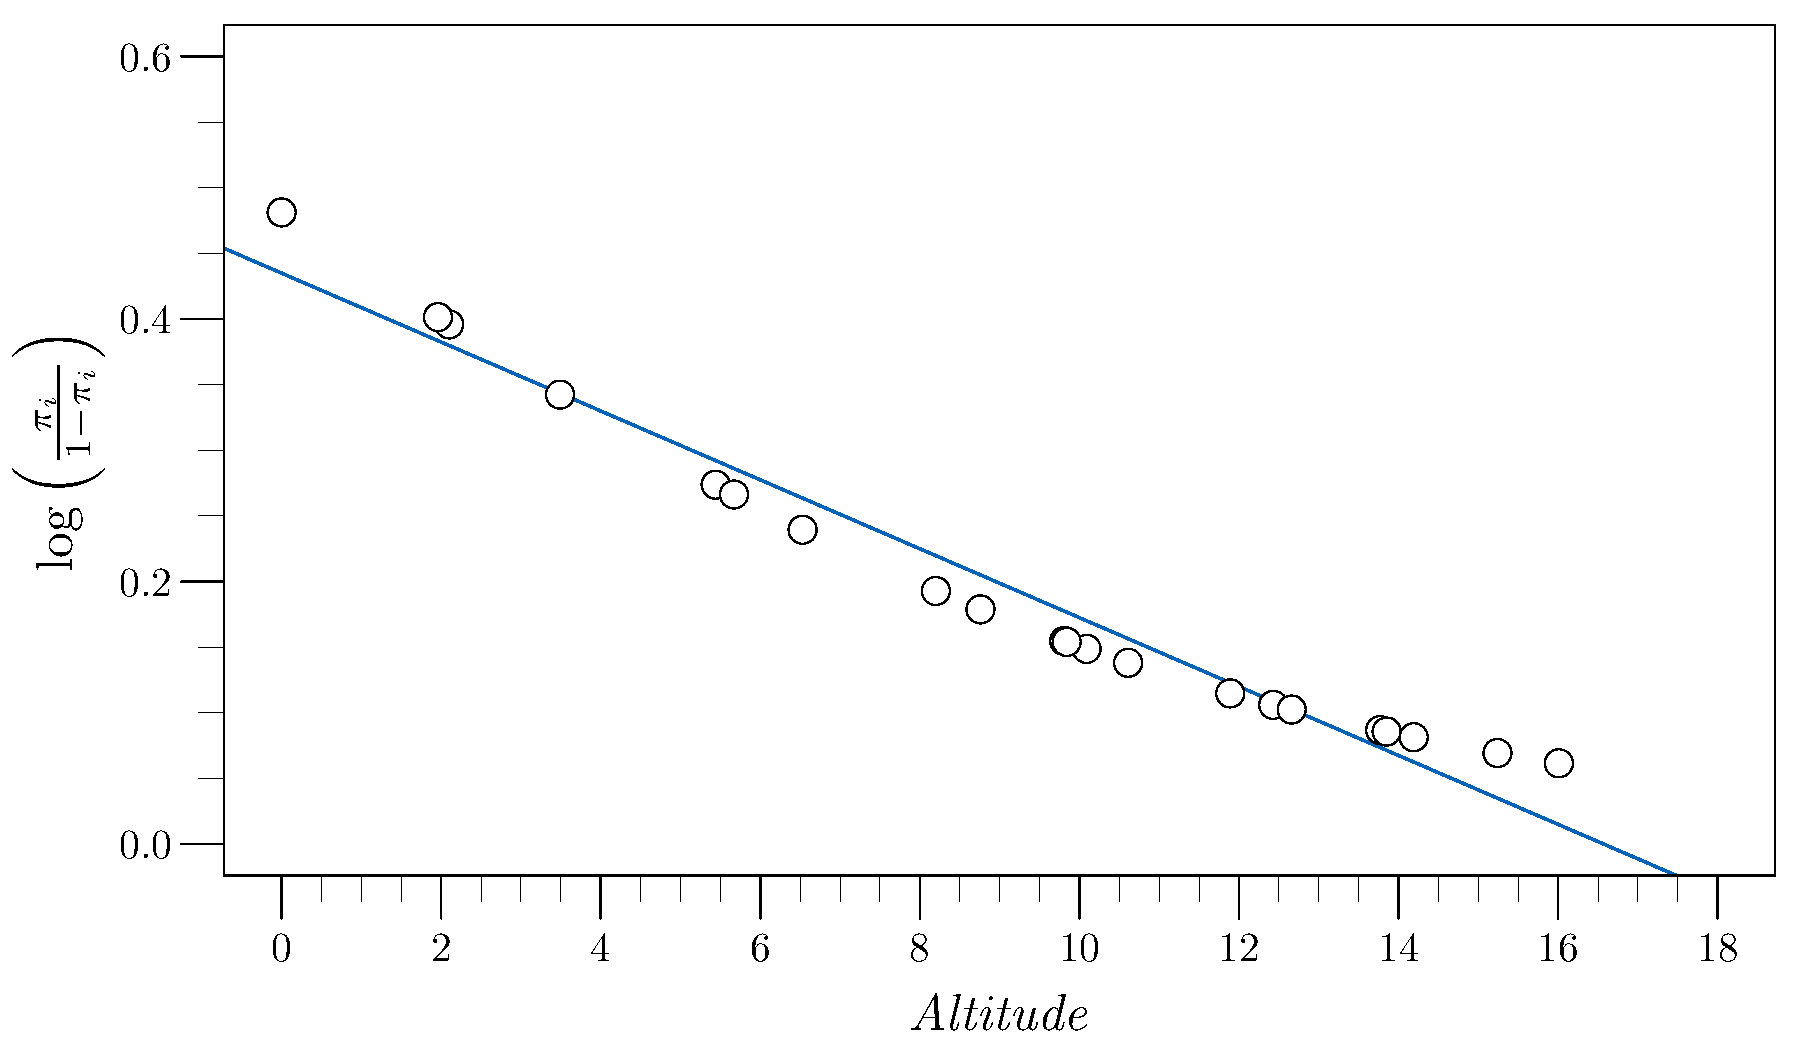
\includegraphics{images/altitude.pdf}
\end{adjustbox}
\caption[Relationship between transmission determinant \textit{Altitude} and respective log odds]{Relationship between prevalence of infection and the transmission determinant \textit{Altitude}. Starting at 0 meters, each unit in the \textit{Altitude} axis represents an increment in 100 meters high.}
\label{fig:altitude_curve}
\end{figure}

For inference purposes, the transmission determinants presented were separated into two different groups.
The first group encompassed the `demographical determinants', all variables characterising the environmental effects and individual characteristics that influenced the outcome.
Risk factors \textit{Transect}, \textit{Altitude}, \textit{AgeGp}, \textit{Gender}, and \textit{EthGp} belong in this group.
A second group identified the `exposure antigens', \textit{MSP1}, \textit{MSP2}, and \textit{AMA1}.
This approach allowed the creation of a first set of models and explain prevalence of infection based exclusively on demographical variables.
Afterwards, the more informative systematic structure was selected and used as reference when adding the exposure factors.
The addition of exposure antigens can be used to indicate the level of exposure to malaria parasites (Table \ref{tab:glm.formulas}).
%The antigens presented mostly work as markers for malaria exposure rather than conferring a noticeable immunological uplift \cite{}, the impact in prevalence reduction is not major.

\begin{table}[ht!]
\centering
\caption[Structure of systematic components used in the GLMs]{Structure of all GLMs' systematic components created, with respective degrees of freedom. Each model assumes probability of infection as response variable. Models \texttt{fit1} to \texttt{fit3} exclusively use variables from the demographical determinants. The following models add variables from the exposure antigens. The exposure transmission determinants are added in order, first individually (models \texttt{fit4} through \texttt{fit6}), and then pairing them up in two (\texttt{fit7}, \texttt{fit8}, and \texttt{fit9}). The last two models (\texttt{fit10} and \texttt{fit11}) add all three exposure factors to the \texttt{fit2} and \texttt{fit3} systematic structures.}
\label{tab:glm.formulas}
\begin{adjustbox}{width=\linewidth}
\begin{tabular}{llc} 
\toprule
Model   &  \multicolumn{1}{c}{Terms fitted in model}   &   d.f  \\
\midrule
\texttt{fit1}   & \textit{Altitude} + \textit{AgeGp} + \textit{Gender} + \textit{EthGp} + \textit{Transect}   & 5045   \\
\texttt{fit2}   & \textit{Altitude} $\times$ \textit{AgeGp} + \textit{Gender} + \textit{EthGp} + \textit{Transect}   & 5043   \\
\texttt{fit3}   & \textit{Altitude} $\times$ \textit{AgeGp} + \textit{Gender} + \textit{EthGp} $\times$ \textit{Transect}   & 5039   \\
\texttt{fit4}   & \textit{Altitude} $\times$ \textit{AgeGp} + \textit{Gender} + \textit{EthGp} + \textit{Transect} + \textit{MSP2}  & 5042   \\
\texttt{fit5}   & \textit{Altitude} $\times$ \textit{AgeGp} + \textit{Gender} + \textit{EthGp} + \textit{Transect} + \textit{MSP1}   & 5042   \\
\texttt{fit6}   & \textit{Altitude} $\times$ \textit{AgeGp} + \textit{Gender} + \textit{EthGp} + \textit{Transect} + \textit{AMA1}   & 5042   \\
\texttt{fit7}   & \textit{Altitude} $\times$ \textit{AgeGp} + \textit{Gender} + \textit{EthGp} + \textit{Transect} + \textit{MSP1} + \textit{MSP2}  & 5041   \\
\texttt{fit8}   & \textit{Altitude} $\times$ \textit{AgeGp} + \textit{Gender} + \textit{EthGp} + \textit{Transect} + \textit{MSP2} + \textit{AMA1}  & 5041   \\
\texttt{fit9}   & \textit{Altitude} $\times$ \textit{AgeGp} + \textit{Gender} + \textit{EthGp} + \textit{Transect} + \textit{MSP1} + \textit{AMA1}   & 5041   \\
\texttt{fit10}   & \textit{Altitude} $\times$ \textit{AgeGp} + \textit{Gender} + \textit{EthGp} + \textit{Transect} + \textit{MSP1} + \textit{MSP2} + \textit{AMA1}   & 5040   \\
\texttt{fit11}   & \textit{Altitude} $\times$ \textit{AgeGp} + \textit{Gender} + \textit{EthGp} $\times$ \textit{Transect} + \textit{MSP1} + \textit{MSP2} + \textit{AMA1}   & 5036   \\
\bottomrule
\end{tabular}
\end{adjustbox}
\end{table}

The first structure built, \texttt{fit1}, described malaria prevalence as a function of all demographical determinants with no interactions considered.
%Systematic component fit2 uses the logarithmic transformation of \textit{Altitude}.
%This transformation, firstly thought to help reducing the variability of the data, turned out less impactful than the original risk factor used in fit1, being discarded on the following models.
When recreating malaria prevalence over different time points, the age (or in this case the age group) of an individual is an important risk factor to consider, as it can be a categorical proxy for time of exposure.
%The constant exposure or recurrent infections to endemic malaria causes individuals to develop protective immunity and consequently reducing its prevalence rate at older age groups.
With \textit{Altitude} being a proxy for transmission intensity, the empirical association between this variable and \textit{AgeGp} (\texttt{fit2} and \texttt{fit3}) was expected to more accurately represent the altitude-dependent prevalence values.
% to recreate a peak-shift effect on the altitude-dependent prevalence values.
Under this interaction, the prevalence of infection should present higher values at age group 1$-$4, decreasing to lower estimates until the higher age group 15$-$45.
However, the maximum prevalence reached depends on the continuous \textit{Altitude}, as lower altitude sites have higher transmission intensities recorded.
With each transect mostly represented by a single ethnic group, the structure from \texttt{fit3} recreated the association between variables \textit{EthGp} and \textit{Transect}.

Afterwards, the addition of exposure variables onto the models was made gradually.
Starting at \texttt{fit4}, the exposure antigens were added to the previous model structure from \texttt{fit2}.
First, a single exposure transmission determinant was added to the model.
Factor \textit{MSP2} was added in \texttt{fit4}, \textit{MSP1} in \texttt{fit5}, and \textit{AMA1} was added in \texttt{fit6}.
The comparison of the three models should clarify for a better understanding of how sensitive the antigens are to the presence of infection (their immunogenicity).
%immunogenic they are (i.e. how quickly the antigens react upon exposure to malaria).
Using \texttt{fit2}'s demographical structure, models \texttt{fit7}, \texttt{fit8}, and \texttt{fit9}, added two exposure factors.
Systematic component from \texttt{fit7} included both \textit{MSP1} and \textit{MSP2}, fit8 incorporated \textit{MSP2} and \textit{AMA1}, and \texttt{fit9} built \textit{MSP1} and \textit{AMA1}.
These models functioned as an intermediary complement between the addition of a single antigen factor, and the inclusion of all three.
The order by which the exposure variables were included was based on previous knowledge that specific antigens MSP1 and AMA1 are more impactful than MSP2.
Finally, \texttt{fit10} included all exposure risk factors into \texttt{fit2}'s systematic structure.
The systematic component \texttt{fit11} then extended all three exposure antigens onto the demographical systematic structure from \texttt{fit3}, with a relation between \textit{EthGp} and \textit{Transect}.
%Models fit5 to fit11 are extensions of the peak-shift model fit3, with model fit12 deriving from the structure of the demographical model fit4.
%Models fit5, fit6, and fit7, add each antigen variable individually and can be used to compare the influence each one as on the information gained.
%Since all antigens presented mostly work as markers for malaria exposure rather than conferring a noticeable immunological uplift \cite{}, their impact in prevalence reduction should not be major.
%The structures from fit8, fit9, and fit10, add different pairs of antigens, with fit11 adding all three variables.
%Model fit12 adopted the same idea from the previously constructed fit4, relating variables \textit{EthGp} and \textit{Transect}.

All systematic components were then fitted using three link functions, logistic, probit, and complementary log-log, for a total of 33 possible GLMs (Table \ref{tab:glm.comparison}).
Information criteria (AIC and BIC) and area under the ROC curve (AUC) were the measures used to compare the produced results and select the overall best GLM.
AUC reflected mostly the information gained by the addition of different variables.
This criterion remained unchanged for models possessing the same systematic component structures, simply reflecting the discriminating power of each model.
To compare models built with an equal structure, that only varied their respective link functions, values of AIC and BIC were used.
Since the penalty parameter from the criteria remained unchanged for models with same systematic components (parameters seen in equations (\ref{eq:aic}) and (\ref{eq:bic})), the lowest produced value depended only on the likelihood value given by each associated link function.
The GLMs were tested for their goodness-of-fit using the Hosmer-Lemeshow test statistic with ten deciles of risk groups, and all test statistics originated from equation (\ref{eq:cressie.read}), considering a similar number of classes.
\newpage

Under the systematic component from \texttt{fit1}, the best fitted GLM linked the outcome to its predictors via the cloglog link function.
Assessing the three GLMs from \texttt{fit1}, this model presented the lowest AIC and BIC values recorded.
Complementary, it also had the highest AUC value.
% Despite the link function used, results from the goodness-of-fit tests all suggest a poor fit.
%The use of the logarithmic transformation in fit2 produces higher values of AIC and BIC and lower AUC, suggesting a lesser adjusted model, granting reduced information when compared to the cloglog GLM fit1.
Models adjusted with both \texttt{fit2} and \texttt{fit3} presented best estimated results when the probit link function was used.
The use of an interaction between \textit{Altitude} and \textit{AgeGp} in these models showed an increase in information gain, reaching AUC values above 0.78.
Comparing both probit models, \texttt{fit2} appeared the better option, thus discarding the \textit{EthGp}$-$\textit{Transect} interaction.
% even though its goodness-of-fit tests present p-values $>0.05$.% suggesting lack of association between the covariates.

All models where exposure antigens were added presented better comparative results when the logistic link function was used.
The AIC and BIC values from the ordered models increased gradually, as more transmission determinants were added.
Model created using the systematic components \texttt{fit10} and \texttt{fit11}, reached estimated values of AUC above 0.80.
Comparing the logistic models \texttt{fit4}, \texttt{fit5}, and \texttt{fit6} suggested \textit{AMA1} (\texttt{fit6}) to be the more informative factor, within the analysed antigens.
Indeed, \texttt{fit6} described better the outcome using the same demographical structure as the other two antigens, also corroborating the values obtained for the AMA1 antigen in the analysis of deviance (Table \ref{tab:risk.factors}).
Factor \textit{MSP1} (\texttt{fit5}) was the second more informative, with \textit{MSP2} (\texttt{fit4}) being the one granting the least information to the models.
Logistic models \texttt{fit7}, \texttt{fit8}, and \texttt{fit9} consolidated this information, as both GLMs with the lesser informative transmission determinant \textit{MSP2} showed reduced information.
The models' analysis made from the majority of the goodness-of-fit results suggested the logistic \texttt{fit8} and \texttt{fit9} results did not depart from the model, not rejecting the null hypothesis.
% Although the logistic models present better values on the comparison methods, few appear to be significantly well adjusted at 5\% significance level.

Similarly to the comparison between the two probit models \texttt{fit2} and \texttt{fit3}, the logistic models \texttt{fit10} and \texttt{fit11} were compared one against the other.
Having similar values for AUC, the overall lower AIC and BIC results from the single interaction model identified it as the more parsimonious GLM built.
The logistic GLM \texttt{fit10} presented good performances from the comparison methods, although its p-values from the Hosmer-Lemeshow goodness-of-fit test statistic showed some evidence for lack of fit (p-value$=0.016$).
The test indicated the model to be poorly adjusted to the data, contrarily to the rest.
Regardless of this result, and with the main objective being to build the best possible descriptive model, the logistic \texttt{fit10} was the selected model.
%Results from Pearson's $\chi^2$ validate the model as having a significant association between the variables, with all other not rejecting the null hypothesis.
%The selected model requires then further analyses and adjustments to become more parsimonious, while maintaining its with good predictive power margin.

\begin{table}[H]
\centering
\caption[Comparison and goodness-of-fit results for all constructed GLMs]{Results for the constructed GLMs, grouped by the trio of link functions applied on each structure. Each model presents values of information criteria (AIC and BIC), and AUC, as well as results for the goodness-of-fit test statistics: Hosmer-Lemeshow with 10 deciles of risk group (C$_{HL}^{2}$), Pearson $\chi^{2}$ (X$^{2}$), log-likelihood ratio statistic (G$^{2}$), Freeman-Tukey statistic (T$^{2}$), Neyman modified $\chi^{2}$ (NM$^{2}$), and modified log-likelihood ratio statistic (GM$^{2}$). A bold font indicates the best AIC and BIC for fit.}
\begin{adjustbox}{width=\linewidth}
\label{tab:glm.comparison}
\begin{tabular}{clcccccccccc}
\toprule
\multirow{2}{*}{Model}   & \multirow{2}{*}{Link}   & \multicolumn{3}{c}{Comparison methods}   &   & \multicolumn{6}{c}{Goodness-of-fit}   \\
\cmidrule{3-5}\cmidrule{7-12}
       &           & AIC       & BIC       & AUC     &   & C$_{HL}^{2}$ & X$^{2}$  & G$^{2}$  & T$^{2}$  & NM$^{2}$ & GM$^{2}$ \\ 
\midrule
%fit1   & logit     & 4221.24   & 4306.12   & 0.778   &   & 0.455    & 0.757   & 0.754   & 0.753   & 0.749   & 0.752   \\
%       & probit    & 4224.02   & 4308.89   & 0.778   &   & 0.661    & 0.901   & 1.000   & 0.902   & 0.904   & 0.409   \\
%       & cloglog   & 4218.74   & 4303.62   & 0.778   &   & 0.143    & 0.403   & 0.397   & 0.392   & 0.378   & 0.387   \\
%fit2   & logit     & 4256.04   & 4340.92   & 0.772   &   & 0.607    & 0.859   & 0.859   & 0.860   & 0.860   & 0.860   \\
%       & probit    & 4257.25   & 4342.12   & 0.772   &   & 0.712    & 0.916   & 1.000   & 0.916   & 0.917   & 0.528   \\
%       & cloglog   & 4253.83   & 4338.70   & 0.772   &   & 0.418    & 0.697   & 0.707   & 0.689   & 0.679   & 0.670   \\
%fit3   & logit     & 4190.80   & 4288.73   & 0.782   &   & 0.359    & 0.665   & 0.667   & 0.668   & 0.670   & 0.669   \\
%       & probit    & 4188.80   & 4286.73   & 0.782   &   & 0.299    & 0.568   & 0.525   & 0.548   & 0.524   & 0.571   \\
%       & cloglog   & 4195.65   & 4293.58   & 0.782   &   & 0.641    & 0.820   & 0.559   & 0.801   & 0.779   & 0.990   \\
%fit4   & logit     & 4194.48   & 4318.52   & 0.783   &   & 0.276    & 0.576   & 0.576   & 0.575   & 0.573   & 0.575   \\
%       & probit    & 4193.65   & 4317.70   & 0.783   &   & 0.478    & 0.760   & 0.706   & 0.760   & 0.760   & 0.813   \\
%       & cloglog   & 4195.97   & 4320.02   & 0.783   &   & 0.041    & 0.175   & 0.032   & 0.170   & 0.161   & 0.683   \\
%fit5   & logit     & 4145.53   & 4249.99   & 0.788   &   & 0.676    & 0.856   & 0.855   & 0.855   & 0.854   & 0.855   \\
%       & probit    & 4146.00   & 4250.46   & 0.788   &   & 0.560    & 0.765   & 0.859   & 0.769   & 0.771   & 0.676   \\
%       & cloglog   & 4150.52   & 4254.98   & 0.788   &   & 0.329    & 0.587   & 0.122   & 0.576   & 0.565   & 1.000   \\
%fit6   & logit     & 4134.33   & 4238.79   & 0.793   &   & 0.007    & 0.039   & 0.038   & 0.037   & 0.034   & 0.036   \\
%       & probit    & 4135.47   & 4239.93   & 0.793   &   & 0.022    & 0.082   & 0.058   & 0.079   & 0.075   & 0.107   \\
%       & cloglog   & 4143.88   & 4248.34   & 0.793   &   & 0.015    & 0.072   & 0.004   & 0.070   & 0.066   & 0.737   \\
%fit7   & logit     & 4112.50   & 4216.96   & 0.794   &   & 0.060    & 0.164   & 0.160   & 0.158   & 0.149   & 0.156   \\
%       & probit    & 4114.18   & 4218.64   & 0.794   &   & 0.152    & 0.326   & 0.354   & 0.322   & 0.315   & 0.293   \\
%       & cloglog   & 4118.25   & 4222.71   & 0.794   &   & 0.040    & 0.129   & 0.017   & 0.115   & 0.098   & 0.589   \\
%fit8   & logit     & 4107.09   & 4218.08   & 0.795   &   & 0.029    & 0.081   & 0.074   & 0.070   & 0.055   & 0.065   \\
%       & probit    & 4109.29   & 4220.28   & 0.795   &   & 0.004    & 0.013   & 0.013   & 0.016   & 0.016   & 0.019   \\
%       & cloglog   & 4116.52   & 4227.51   & 0.795   &   & 0.018    & 0.066   & 0.003   & 0.044   & 0.026   & 0.489   \\
%fit9   & logit     & 4087.89   & 4198.88   & 0.797   &   & 0.180    & 0.337   & 0.337   & 0.336   & 0.328   & 0.334   \\
%       & probit    & 4092.61   & 4203.60   & 0.797   &   & 0.019    & 0.056   & 0.112   & 0.071   & 0.083   & 0.045   \\
%       & cloglog   & 4092.59   & 4203.58   & 0.797   &   & 0.371    & 0.600   & 0.139   & 0.575   & 0.548   & 1.000   \\
%fit10  & logit     & 4078.17   & 4189.16   & 0.800   &   & 0.005    & 0.020   & 0.021   & 0.022   & 0.022   & 0.022   \\
%       & probit    & 4081.87   & 4192.86   & 0.800   &   & $<$0.001 & 0.002   & 0.003   & 0.003   & 0.004   & 0.004   \\
%       & cloglog   & 4086.87   & 4197.85   & 0.800   &   & 0.004    & 0.021   & 0.001   & 0.017   & 0.012   & 0.198   \\
%fit11  & logit     & 4062.81   & 4180.33   & 0.801   &   & 0.014    & 0.048   & 0.051   & 0.051   & 0.050   & 0.051   \\
%       & probit    & 4068.41   & 4185.92   & 0.801   &   & $<$0.001 & 0.002   & 0.003   & 0.002   & 0.002   & 0.002   \\
%       & cloglog   & 4070.81   & 4188.33   & 0.801   &   & 0.085    & 0.254   & 0.023   & 0.229   & 0.202   & 1.000   \\
%fit12  & logit     & 4067.07   & 4210.70   & 0.802   &   & 0.014    & 0.045   & 0.049   & 0.051   & 0.050   & 0.051   \\
%       & probit    & 4073.75   & 4217.38   & 0.802   &   & 0.001    & 0.005   & 0.010   & 0.007   & 0.008   & 0.005   \\
%       & cloglog   & 4071.02   & 4214.65   & 0.802   &   & 0.030    & 0.095   & 0.032   & 0.100   & 0.100   & 0.286   \\
\texttt{fit1}   & logit              & 4221.24   & 4306.12   & 0.778   &   & 0.057   & 0.374   & 0.374   & 0.372   & 0.362   & 0.370   \\
       & probit             & 4224.02   & 4308.89   & 0.778   &   & 0.054   & 0.382   & 0.650   & 0.378   & 0.365   & 0.186   \\
       & \textbf{cloglog}   & 4218.74   & 4303.62   & 0.778   &   & 0.097   & 0.443   & 0.438   & 0.433   & 0.417   & 0.428   \\
\texttt{fit2}   & logit              & 4190.80   & 4288.73   & 0.782   &   & 0.059   & 0.258   & 0.251   & 0.245   & 0.221   & 0.238   \\
       & \textbf{probit}    & 4188.80   & 4286.73   & 0.782   &   & 0.104   & 0.327   & 0.281   & 0.285   & 0.228   & 0.287   \\
       & cloglog            & 4195.65   & 4293.58   & 0.782   &   & 0.026   & 0.180   & 0.051   & 0.161   & 0.130   & 0.412   \\
\texttt{fit3}   & logit              & 4194.48   & 4318.52   & 0.783   &   & 0.028   & 0.132   & 0.138   & 0.138   & 0.127   & 0.136   \\
       & \textbf{probit}    & 4193.65   & 4317.70   & 0.783   &   & 0.002   & 0.018   & 0.021   & 0.023   & 0.019   & 0.024   \\
       & cloglog            & 4195.97   & 4320.02   & 0.783   &   & 0.094   & 0.273   & 0.215   & 0.310   & 0.315   & 0.425   \\
\texttt{fit4}   & \textbf{logit}     & 4145.53   & 4249.99   & 0.788   &   & 0.585   & 0.877   & 0.885   & 0.888   & 0.898   & 0.892   \\
       & probit             & 4146.00   & 4250.46   & 0.788   &   & 0.854   & 0.970   & 0.983   & 0.969   & 0.967   & 0.949   \\
       & cloglog            & 4150.52   & 4254.98   & 0.788   &   & 0.334   & 0.697   & 0.312   & 0.710   & 0.717   & 0.987   \\
\texttt{fit5}   & \textbf{logit}     & 4134.33   & 4238.79   & 0.793   &   & 0.034   & 0.164   & 0.168   & 0.168   & 0.160   & 0.167   \\
       & probit             & 4135.47   & 4239.93   & 0.793   &   & 0.008   & 0.053   & 0.033   & 0.036   & 0.019   & 0.039   \\
       & cloglog            & 4143.88   & 4248.34   & 0.793   &   & 0.054   & 0.234   & 0.035   & 0.237   & 0.228   & 0.808   \\
\texttt{fit6}   & \textbf{logit}     & 4112.50   & 4216.96   & 0.794   &   & 0.205   & 0.472   & 0.470   & 0.465   & 0.433   & 0.457   \\
       & probit             & 4114.18   & 4218.64   & 0.794   &   & 0.536   & 0.814   & 0.834   & 0.811   & 0.803   & 0.786   \\
       & cloglog            & 4118.25   & 4222.71   & 0.794   &   & 0.180   & 0.491   & 0.152   & 0.448   & 0.388   & 0.864   \\
\texttt{fit7}   & \textbf{logit}     & 4107.09   & 4218.08   & 0.795   &   & 0.013   & 0.066   & 0.044   & 0.032   & 0.007   & 0.022   \\
       & probit             & 4109.29   & 4220.28   & 0.795   &   & 0.011   & 0.050   & 0.047   & 0.049   & 0.030   & 0.049   \\
       & cloglog            & 4116.52   & 4227.51   & 0.795   &   & 0.014   & 0.087   & 0.006   & 0.043   & 0.011   & 0.211   \\
\texttt{fit8}   & \textbf{logit}     & 4087.89   & 4198.88   & 0.797   &   & 0.267   & 0.543   & 0.493   & 0.464   & 0.358   & 0.431   \\
       & probit             & 4092.61   & 4203.60   & 0.797   &   & 0.174   & 0.388   & 0.536   & 0.429   & 0.441   & 0.331   \\
       & cloglog            & 4092.59   & 4203.58   & 0.797   &   & 0.275   & 0.579   & 0.208   & 0.477   & 0.354   & 0.822   \\
\texttt{fit9}   & \textbf{logit}     & 4078.17   & 4189.16   & 0.800   &   & 0.019   & 0.084   & 0.102   & 0.108   & 0.112   & 0.111   \\
       & probit             & 4081.87   & 4192.86   & 0.800   &   & 0.004   & 0.021   & 0.030   & 0.034   & 0.036   & 0.037   \\
       & cloglog            & 4086.87   & 4197.85   & 0.800   &   & 0.037   & 0.157   & 0.024   & 0.154   & 0.137   & 0.605   \\
\texttt{fit10}  & \textbf{logit}     & 4062.81   & 4180.33   & 0.801   &   & 0.016   & 0.089   & 0.100   & 0.103   & 0.100   & 0.104   \\
       & probit             & 4068.41   & 4185.92   & 0.801   &   & 0.001   & 0.010   & 0.018   & 0.017   & 0.016   & 0.014   \\
       & cloglog            & 4070.81   & 4188.33   & 0.801   &   & 0.012   & 0.085   & 0.009   & 0.052   & 0.023   & 0.220   \\
\texttt{fit11}  & \textbf{logit}     & 4067.07   & 4210.70   & 0.802   &   & 0.097   & 0.276   & 0.260   & 0.247   & 0.186   & 0.230   \\
       & probit             & 4073.75   & 4217.38   & 0.802   &   & 0.001   & 0.008   & 0.023   & 0.019   & 0.022   & 0.015   \\
       & cloglog            & 4071.02   & 4214.65   & 0.802   &   & 0.072   & 0.265   & 0.129   & 0.259   & 0.235   & 0.464   \\
\bottomrule
\end{tabular}
\end{adjustbox}
\end{table}


%%%%%%%%%%%%%%%%%%%%%%%%
% RESULTS AND ANALYSES %
%%%%%%%%%%%%%%%%%%%%%%%%
\section{Model inferences}

With the majority of the goodness-of-fit test statistics suggesting no evidence against the null hypothesis of good fit, no further adjustments were made to the logistic model \texttt{fit10} (Table \ref{tab:fit11.glm}).
% in order to ameliorate the model's \textcolor{red}{parsimony or its (already adequate) predictive power -- isto valerá a pena?} (Table \ref{tab:fit11.glm}).
Assessing the AUC of approximately 0.801, its optimal cutoff for sensitivity and specificity were calculated as 0.786 and 0.691, respectively (Figure \ref{fig:roc_curve}).
\\

% Most goodness-of-fit test statistics suggested a good fit from the logistic model fit10.
% However, some adjustments could still be done to ameliorate the model's parsimony, while maintaining its good predictive power.
% Factor \textit{Gender}, identified from the start as a non significant variable, and thought to not play a part in the malaria infection outcome, was removed.
% Its removal produced a well adjusted model (Table \ref{tab:fit11.glm}), with significant results in all test statistics ($\text{C}_{HL}^2=21.482,\ \text{p-value}=0.006;\ \text{X}^2=19.021,\ \text{p-value}=0.040;\ \text{G}^2=19.144,\ \text{p-value}=0.038;\ \text{T}^2=19.350\ ,\text{p-value}=0.036;\ \text{NM}^2=20.575,\ \text{p-value}=0.024;\ \text{GM}^2=19.654,\ \text{p-value}=0.033$).
% AIC value slightly increased, while the more sensible BIC decreased (4063.43 and 4174.42, respectively), thus confirming the quality of the model, when fit to the data.
% For this new prevalence model, estimated AUC maintained at the approximately 0.80, a good predictive power (Figure \ref{fig:roc_curve}).
% The model had an optimal cutoff when sensitivity was equal to 0.778 and specificity was 0.706.
%suggest it does not play a part in the malaria infection, being identified as a non-significant variable.
%Its removal originates a more parsimonious and well adjusted model (Table \ref{tab:fit11.glm}).
%This new prevalence model slightly increases its AIC value, while decreasing the more sensible BIC, for respective values 4063.40 and 4174.4.
%All goodness-of-fit tests present p-values below the fixed 0.05, confirming the quality of the model when fit to the data .

\begin{figure}[H]
\center
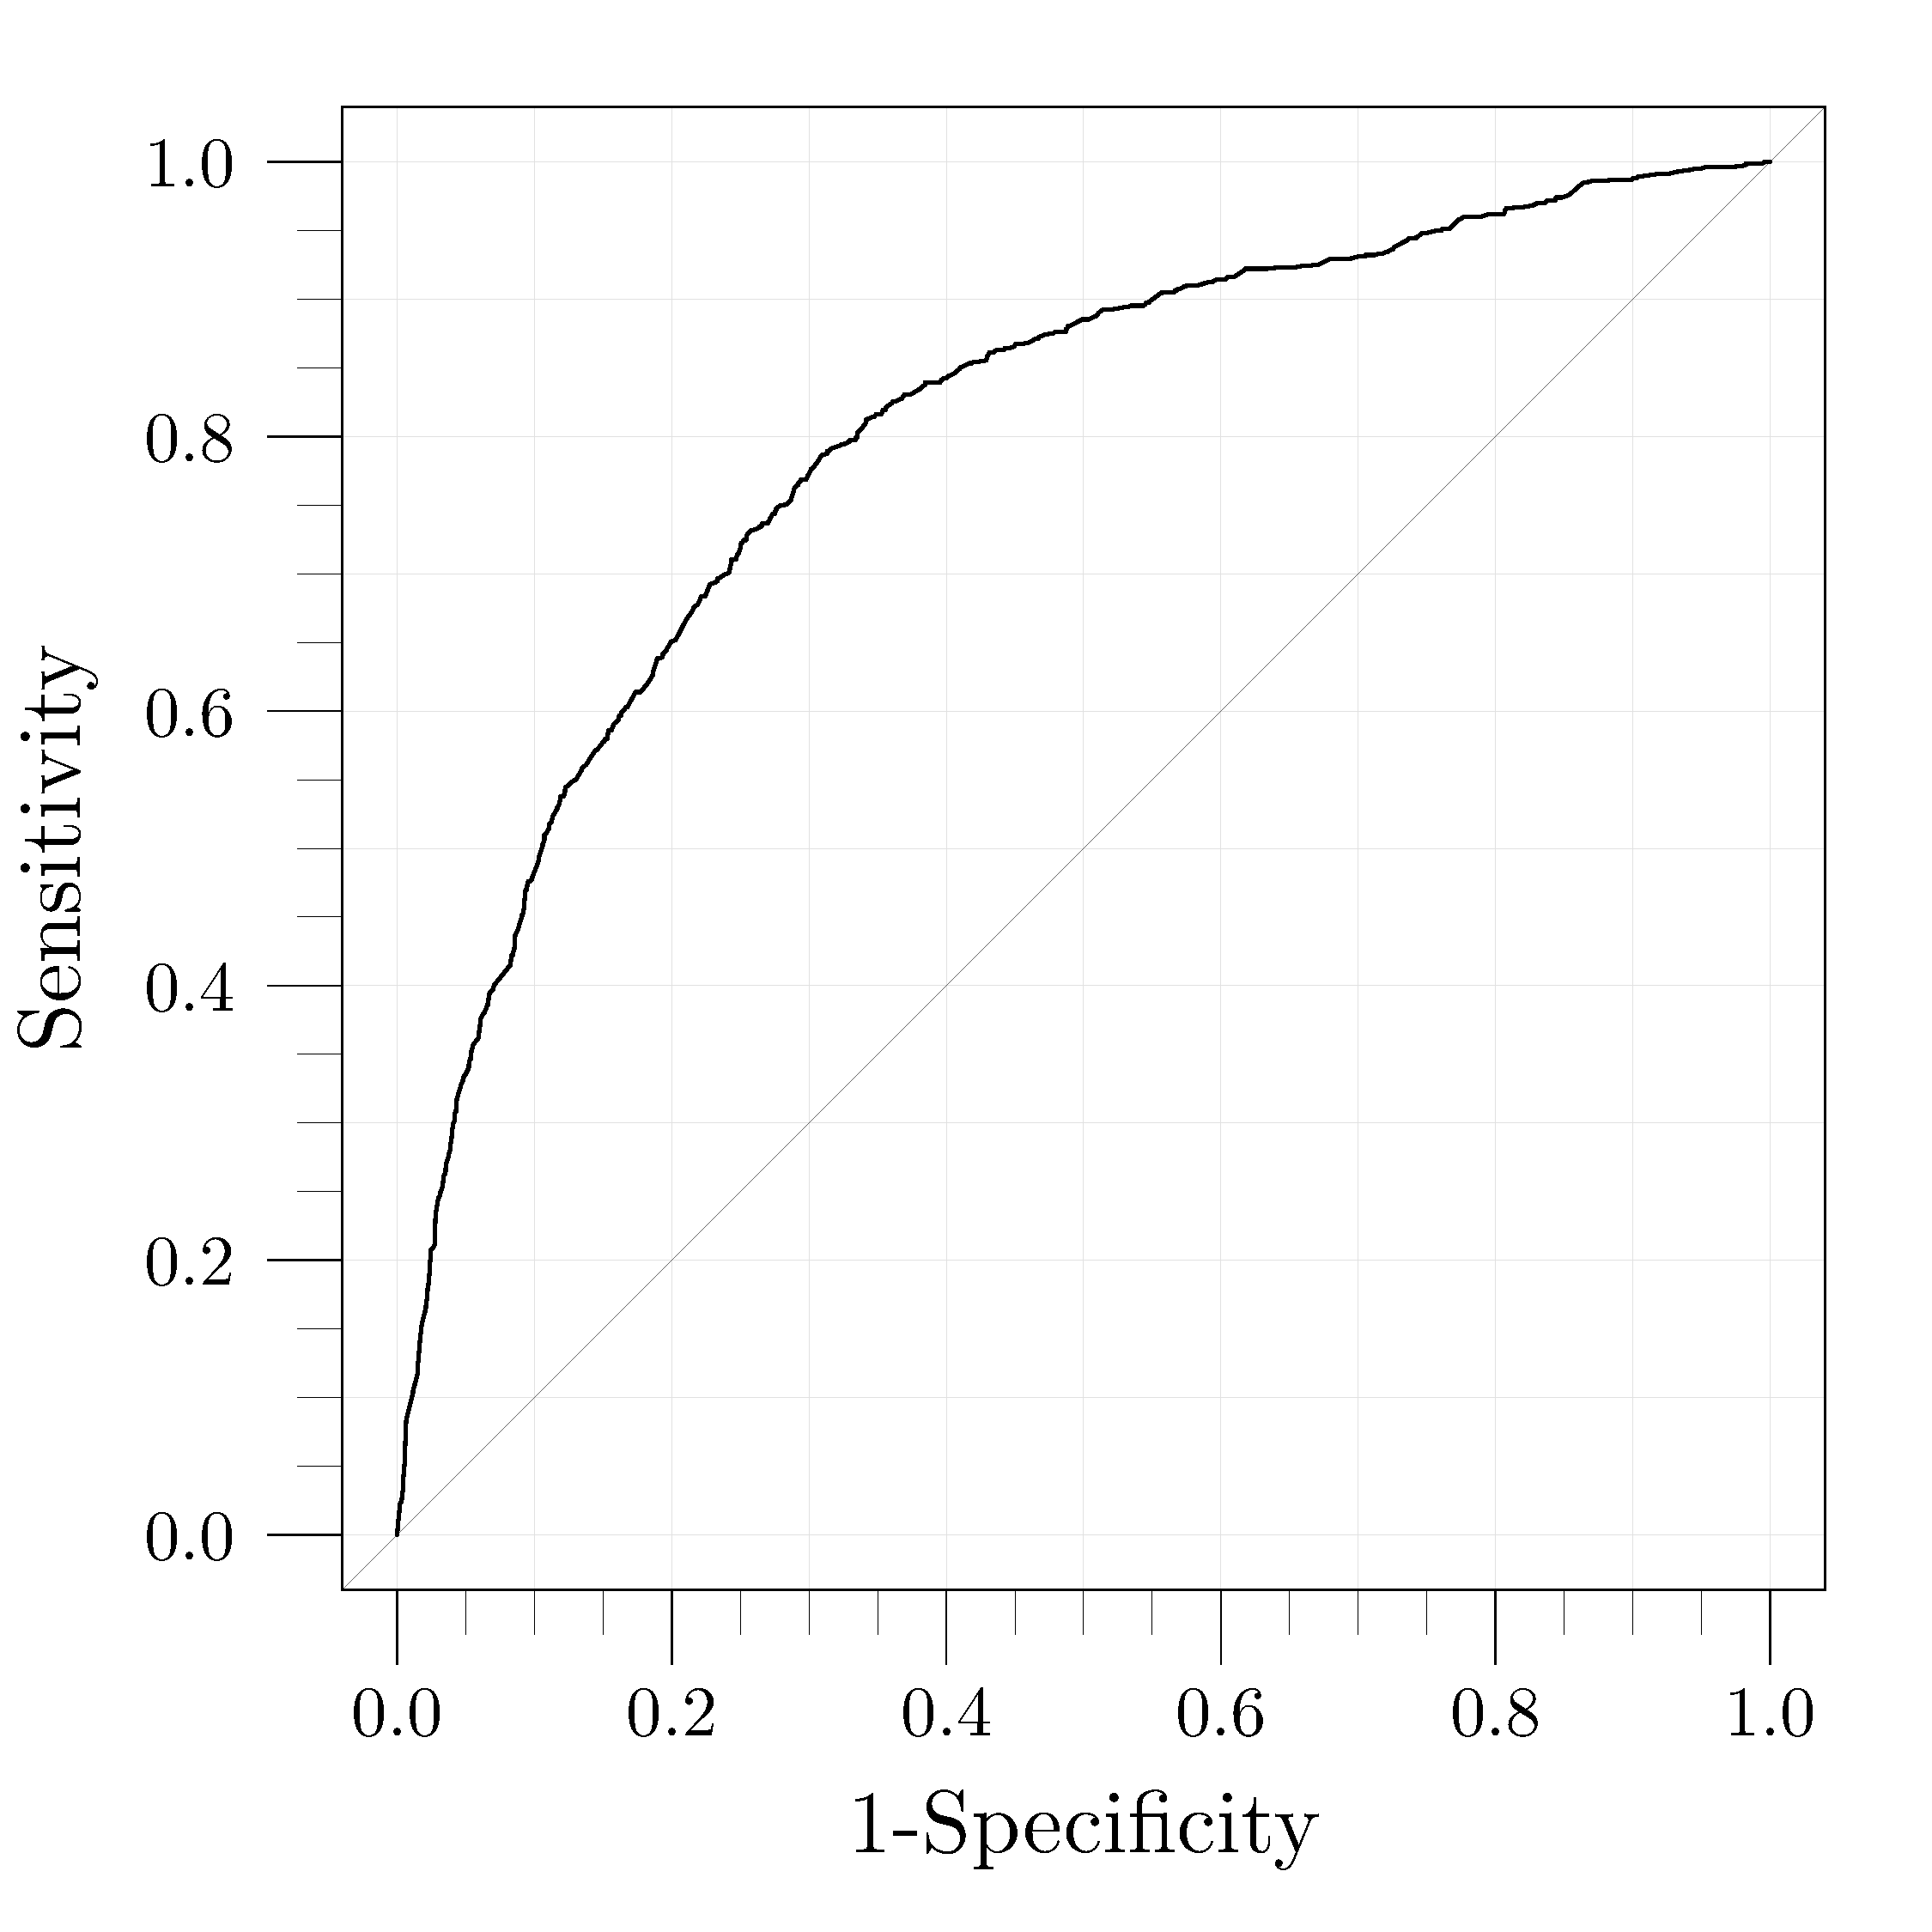
\includegraphics[width=9.5cm,height=9.5cm]{images/ROC_curve.pdf}
\caption[ROC curve of the selected GLM]{ROC curve of the logit model \texttt{fit10} ($\text{AUC}=0.801$). Maximum discrimination for values of sensitivity equal to 0.786 and specificity equal to 0.691.}
\label{fig:roc_curve}
\end{figure}

The logit link function facilitated further epidemiological inferences of the coefficients of the model, allowing for the interpretation of the explanatory variables in terms of odds ratio \cite{collet2003modelling}.
% With the model's parameters, and their respective standard errors, the odds of malaria infection occurrence to an individual can be obtained.
This is, comparing the odds of possible malaria infection when in relation to a similar individual that has a single variation in one of its variables.
%The standard error of the estimated of $\widehat{\beta}_1$ will be the standard error of the estimated log odds ratio, that is $\text{se}(\widehat{\beta}_1)=\text{se}(\log(e^{\beta_1}))$. With this results, an approximate 95\% confidence interval for the true odds ratio can be calculated by the expression XXX.\\
%The fact that this interval includes the unity suggests that the risk of infection occurring in persons XXX is not significantly different from those in the baseline level.
The analysis of the more significant transmission determinants and their respective odds ratios can create an association between the variations in malaria transmission intensity across the different situations that characterise the data.
%Investigating which are the significant risk factors that when combined cause a rise in prevalence of infection.
%Prevalence=probability of malaria infection occurre=the risk disease occurrence.\\
%Number of cases of the disease that occur given a period.\\
%The main purpose of estimating risks is to be able to make comparisons between the risk of disease at different levels of an risk factor, and thereby assess the association between the disease and that risk factor.\\
\newpage

\begin{table}[ht!]
\centering
\caption[Adjusted logistic GLM \texttt{fit10}]{Adjusted logistic GLM \texttt{fit10} with respective significant variables estimates, standard error and p-value. Odds ratio are given in relation to the indicator level of each transmission determinant (the odds ratios for these levels are equal to 1.00). For reference, the baseline level from the categorical demographical determinants are here indicated: $\textit{AgeGp}_{1-4}$, $\textit{Gender}_{Female}$, $\textit{EthGp}_{Other}$, and $\textit{Transect}_{WU3}$.}
\label{tab:fit11.glm}
\begin{adjustbox}{width=\linewidth}
% \begin{tabular}{ccrcrcc} 
% \toprule
% \multicolumn{1}{c}{Coefficient} & \multicolumn{1}{c}{\begin{tabular}[c]{@{}c@{}}Factor\\level\end{tabular}} & \multicolumn{1}{c}{\begin{tabular}[c]{@{}c@{}}Parameter\\estimate\end{tabular}} & \multicolumn{1}{c}{\begin{tabular}[c]{@{}c@{}}Standard\\error\end{tabular}} & \multicolumn{1}{c}{p-value} & \multicolumn{1}{c}{Odds ratio} & \multicolumn{1}{c}{\begin{tabular}[c]{@{}c@{}}95\% Confidence\\interval\end{tabular}}  \\ 
% \midrule
% (Intercept)                        & ---           & $-$0.775   & 0.212   & $<$0.001   & 0.46 & (0.30, 0.70)   \\
% \textit{Altitude}                  & ---           & $-$0.148   & 0.019   & $<$0.001   & 0.86 & (0.83, 0.89)   \\
% \textit{AgeGp}                     & 5$-$14        &  0.095     & 0.190   & 0.619      & 1.10 & (0.76, 1.60)   \\
%                                   & 15$-$45       & $-$1.712   & 0.196   & $<$0.001   & 0.18 & (0.12, 0.26)   \\
% \textit{EthGp}                     & Wachaga       &  0.623     & 0.320   & 0.052      & 1.86 & (1.00, 3.51)   \\
%                                   & Wapare        & $-$0.224   & 0.209   & 0.284      & 0.80 & (0.53, 1.21)   \\
%                                   & Wasambaa      &  0.192     & 0.160   & 0.231      & 1.21 & (0.89, 1.66)   \\
% \textit{Transect}                  & Rombo         & $-$0.971   & 0.322   & 0.003      & 0.38 & (0.20, 0.71)   \\
%                                   & N. Pare       & $-$1.478   & 0.337   & $<$0.001   & 0.23 & (0.12, 0.43)   \\
%                                   & S. Pare       & $-$0.420   & 0.247   & 0.089      & 0.66 & (0.40, 1.06)   \\
%                                   & W. Usamb. 1   &  0.463     & 0.214   & 0.030      & 1.59 & (1.04, 2.42)   \\
%                                   & W. Usamb. 2   &  0.014     & 0.212   & 0.946      & 1.01 & (0.67, 1.54)   \\
% \textit{AMA1}                      & 1             &  0.664     & 0.098   & $<$0.001   & 1.94 & (1.60, 2.36)   \\
% \textit{MSP1}                      & 1             &  0.500     & 0.097   & $<$0.001   & 1.65 & (1.36, 1.99)   \\
% \textit{MSP2}                      & 1             &  0.393     & 0.095   & $<$0.001   & 1.48 & (1.23, 1.79)   \\
% \textit{Altitude $\times$ AgeGp}   & 5$-$14        &  0.022     & 0.022   & 0.316      & 1.02 & (0.98, 1.07)   \\
%                                   & 15$-$45       &  0.114     & 0.023   & $<$0.001   & 1.12 & (1.07, 1.17)   \\
% \bottomrule
% \end{tabular}
\begin{tabular}{ccrcrcc} 
\toprule
\multicolumn{1}{c}{Coefficient} & \multicolumn{1}{c}{\begin{tabular}[c]{@{}c@{}}Factor\\level\end{tabular}} & \multicolumn{1}{c}{\begin{tabular}[c]{@{}c@{}}Parameter\\estimate, $\widehat{\beta}$\end{tabular}} & \multicolumn{1}{c}{\begin{tabular}[c]{@{}c@{}}Standard\\error\end{tabular}} & \multicolumn{1}{c}{p-value} & 
\multicolumn{1}{c}{\begin{tabular}[c]{@{}c@{}}Odds ratio,\\$e^{\widehat{\beta}}$\end{tabular}} &
\multicolumn{1}{c}{\begin{tabular}[c]{@{}c@{}}95\% Confidence\\interval\end{tabular}}  \\ 
\midrule
(Intercept)                        & ---           & $-$0.863   & 0.218   & $<$0.001   & 0.42   & (0.28, 0.65)   \\
\textit{Altitude}                  & ---           & $-$0.148   & 0.019   & $<$0.001   & 0.86   & (0.83, 0.89)   \\
\textit{AgeGp}                     & 5$-$14        &    0.112   & 0.190   & 0.555      & 1.12   & (0.77, 1.63)   \\
                                   & 15$-$45       & $-$1.681   & 0.197   & $<$0.001   & 0.19   & (0.13, 0.27)   \\
\textit{Gender}                    & Male          &    0.134   & 0.083   & 0.105      & 1.14   & (0.97, 1.34)   \\
\textit{EthGp}                     & Wachaga       &    0.619   & 0.320   & 0.053      & 1.86   & (1.00, 3.50)   \\
                                   & Wapare        & $-$0.228   & 0.209   & 0.276      & 0.80   & (0.53, 1.20)   \\
                                   & Wasambaa      &    0.194   & 0.160   & 0.226      & 1.21   & (0.89, 1.67)   \\
\textit{Transect}                  & Rombo         & $-$0.956   & 0.322   & 0.003      & 0.38   & (0.20, 0.72)   \\
                                   & N. Pare       & $-$1.470   & 0.337   & $<$0.001   & 0.23   & (0.12, 0.44)   \\
                                   & S. Pare       & $-$0.407   & 0.247   & 0.099      & 0.67   & (0.41, 1.08)   \\
                                   & W. Usamb. 1   &    0.472   & 0.214   & 0.027      & 1.60   & (1.05, 2.44)   \\
                                   & W. Usamb. 2   &    0.028   & 0.212   & 0.894      & 1.03   & (0.68, 1.56)   \\
\textit{AMA1}                      & 1             &    0.666   & 0.099   & $<$0.001   & 1.95   & (1.61, 2.36)   \\
\textit{MSP1}                      & 1             &    0.505   & 0.097   & $<$0.001   & 1.66   & (1.37, 2.00)   \\
\textit{MSP2}                      & 1             &    0.396   & 0.095   & $<$0.001   & 1.49   & (1.23, 1.79)   \\
\textit{Altitude $\times$ AgeGp}   & 5$-$14        &    0.022   & 0.022   & 0.335      & 1.02   & (0.98, 1.07)   \\
                                   & 15$-$45       &    0.114   & 0.023   & $<$0.001   & 1.12   & (1.07, 1.17)   \\
\bottomrule
\end{tabular}
\end{adjustbox}
\end{table}

In Mgome, 111 out of the 225 inhabitants were not infected.
Being the village with the highest prevalence of infection at the moment of sampling, one expected this selected baseline site to present good characteristics that, by comparison, could help to describe the different prevalence amongst all other villages.
% The logistic regression model shows that the risk of developing malaria infection during XXX was XXX times (p-value=XXX) higher in individuals XXX at the moment of sampling, than those who were XXX.
The odds ratio analysis suggested that the odds of an individual developing malaria infection at the reference village's altitude (0 meters, recall Section \ref{sec:4.1}) was significantly higher than those who inhabited any site with a higher altitude ($\widehat{\beta}=−0.148$ and $\text{p-value}<0.001$).
Being a proxy of malaria transmission, each 100 meters increased in altitude granted a reduction in odds of infection of approximately 14\% ($\widehat{OR}=0.86$).
This reduction showed how impactful altitude is, working as a protective factor.
The small confidence interval for the true odds ratio suggested a high precision of the odds of infection.
%This protective odds factor, proxy of malaria transmission intensity, has a small 95\% confidence interval.
% \textcolor{red}{FALAR AQUI DE COMO A VARIÁVEIS CLIMÁTICAS ESTÃO DIRECTAMENTE RELACIONADAS E REPRESENTADAS PELA ALTITUDE.}

% Agegp
Comparing the different age groups, only individuals older than 14 years old appeared to have their odds of infection significantly reduced ($\widehat{\beta}=-1.681$ and $\text{p-value}<0.001$).
This reduction -- $\widehat{OR}=0.19$, the biggest estimated in the categorical transmission determinants -- suggested older individuals were more prepared to live in sites of endemic transmission settings.
These older inhabitants, when in similar conditions as children from the reference level \textit{AgeGp}$_{1-4}$, would had their odds of being infected reduced by 73\% to 87\%.
There was no significant difference from infants to children with ages between 5 and 14 years old.
% The risk from individuals in the second age group ($\text{p-value}=0.619$) seems higher relatively to the first.
% However, with a confidence interval for the true odds ratio containing the unity, this level seems inconclusive, not influencing the prevalence of infection.
% The risk factor \textit{AgeGp}, with two degrees of freedom, estimates the odds ratio of its upper age groups relative to its indicator level.
% The risk of infection for individuals with ages comprehended in the second age group, $\textit{AgeGp}_{5-14}$ ($\text{p-value}=0.619$), shows a small increase of 6\% in prevalence.
% With its respective confidence interval for the true odds ratio ranging from 0.68 to 1.64, this level does not seem to significantly influence the prevalence of infection.
% However, individuals in the the third age group level, $\textit{AgeGp}_{15-45}$ ($\text{p-value}<0.001$), have their risk of infection reduced by 74\% to 88\%, when compared to the reference age group.
% This reduction (the biggest estimated in the categorical risk factors) suggests that individuals older than 14 years old are usually protected enough, and when in similar conditions as children from the first age group, their risk of being infected would be 82 times smaller.
% Gender
The binary risk factor \textit{Gender}, was kept throughout the model's construction.
Ultimately it did not seem to play a significant role influencing prevalence of infection ($\widehat{\beta}=0.134$ and $\text{p-value}=0.105$).

% Ethnic
Assessing the different ethnicities, only the Wachaga ethnic group ($\widehat{\beta}=0.619$ and $\text{p-value}=0.053$) seemed to produce a borderline significant result on the response variable, with $\widehat{OR}=1.86$.
Despite the inclusion of the unity in the estimated confidence interval for the true odds ratio, this level suggested a tendency.
In similar conditions, individuals from this ethnic group would had higher odds infection than someone from the ethnicities found in Mgome, $\textit{EthGp}_{Other}$, at the moment of sampling.
% Maybe by omitting data from some individuals in the analysis could adjust the estimated odds ratio to some extend, and removing the unity from the confidence interval, resulting in some more informative results.
The odds of infection in individuals from the remaining ethnic groups Wapare ($\widehat{\beta}=-0.228$ and $\text{p-value}=0.276$) and Wasambaa ($\widehat{\beta}=0.194$ and $\text{p-value}=0.226$) did not appear significantly different in the analysis.
% , suggest individuals in these ethnic groups have a increased risk of being infected than someone with Other ethnicity, under the same conditions.
% As for the Wapare ethnic group ($\text{p-value}=0.284,\ \text{OR}=0.80$), the relative risk of an individual from this ethnic group being infected is reduced.
% Even though different ethnicities granted different levels of risk of malaria prevalence, the exclusion of data from some individuals in the analysis could adjust the estimated odds ratio to some extend, resulting in some more informative or precise confidence intervals. OUT

% Transect
The covariate \textit{Transect} showed how malaria transmission intensity varied between the two Tanzanian regions, across the different defined transects.
If compared in the same conditions, individuals from the four villages in Rombo ($\widehat{\beta}=-0.956$ and $\text{p-value}=0.003$) had their odds of being infected reduced by 62\% ($\widehat{OR}=0.38$), while villages in the North Pare ($\widehat{\beta}=-1.470$ and $\text{p-value}<0.001$) had their odds reduced by 77\% ($\widehat{OR}=0.23$).
The latter showed the more significant and precise odds reduction.
Similar to the tendency value in $\textit{EthGp}_{Wachaga}$, with the inclusion of the unity within the confidence interval of the true odds ratio, villages belonging to South Pare seem to present reduced odds for malaria infection.
%However, since the confidence interval for the true odds ratio includes the unity, the results fom South Pare can be somewhat inconclusive.
In the Tanga region, West Usambara 1 ($\widehat{\beta}=0.472$ and $\text{p-value}=0.027$) suggested a higher odds of infection relatively to Mgome, having prevalence growing by 1.60 times.
West Usambara 2 ($\widehat{\beta}=0.028$ and $\text{p-value}=0.894$) did not seem to significantly impact prevalence.
% The analysis of the confidence intervals for the true odds ratio in the different transects marked \textit{Transect} as a highly determinant factor for malaria infection.

% AMA1 MSP1 MSP2
The presence of each one of exposure antigens, \textit{AMA1}, \textit{MSP1}, or \textit{MSP2} ($\widehat{\beta}=0.666$, $\widehat{\beta}=0.505$, and, $\widehat{\beta}=0.022$, respectively, all with $\text{p-values}<0.001$), when compared to their respective control level, consistently increased the prevalence as a consequence for exposure ($\widehat{OR}_{AMA1}=1.95$, $\widehat{OR}_{MSP1}=1.66$, $\widehat{OR}_{MSP2}=1.49$, respectively).
This increment suggested how impactful the antigens can be.
Since in normal conditions any non exposed individual is expected to not develop specific antimalarial antibodies, thus not being at risk of becoming infected, the simple detection of an antigen by itself implies a increase on the odds of infection due to exposure.
Depending on the three antigens, odds of infection increased from almost 50\%, when MSP2 was detected, to almost doubling the odds whenever antigen AMA1 was detected in the serum.
%(0.000, 1.02)This interval barely includes the unity, suggesting that the evidence that XXX protects against malaria infection is now significant at about the 5\% level. Omitting the data from some individuals from the analysis could decrease the estimated odds ratio to some extend, resulting in a more informative result.


%%%%%%%%%%%
% SUMMARY %
%%%%%%%%%%%
\section{Summary}

% Primeira frase é conversa fiada...
The identification and study of the primary malaria infection covariates in a region is an approach that can be made as soon as enough variables are collected.
These analyses present some flexibility, as different and more specific transmission determinants can be included for consideration, depending on the study objectives \cite{binka1995risk}.
When overseeing the regions of the Northeast Tanzania, the best combination of transmission determinants through the GLMs helped making inferences about the relative proportion of infected malaria cases across the different sites at the time of sampling.
Also, through the regression coefficient estimates and estimated odds ratio, the relative transmission intensity across the different villages was compared, inferring about impactful determinants that could originate the prevalence estimated and transmission intensity heterogeneity measured.
% In distant or contrasting regions, the identification of the important determinants can potentially lead to hotspots for prevalence of infection.

The application of different categorical variables onto the logistic regression model \texttt{fit10} identified the more susceptible levels to infection.
In the demographical determinants, both \textit{AgeGp} and \textit{Transect} proved to be important categorical risk factors to describe occurrence of infection.
% As the latter can influence the prevalence of infection, the effect of \textit{AgeGp} also reflects the acquired immunity to parasites.
The odds of adults becoming infected with malaria is lower since they might have developed specific immunity throughout periods of recurrent exposure and reinfections.
The impact of these transmission determinants can be related to the geographical conditions of each site, modelling the environment and overall anthropomorphic characteristic of its inhabitants.
Variable \textit{Altitude} also played an important role.
As a proxy for transmission intensity, a value increment in this continuous risk factor can be interpreted as a decrease in temperature and humidity, gradually reducing the number of \textit{Anopheles} mosquitoes, \textit{P. falciparum} transmitters.

Binary variables for the antigen responses presented elevated odds for malaria infection.
All three exposure antigens worked well as stable predictors for malaria exposure, being indirectly influenced by the demographical determinants delineating the level of exposure, and presenting a direct effect in the immunological uplift (aquired immunity) over time gained by an individual \cite{shelton2015genetic}.
With the antigens identified as good indicators for exposure to malaria parasites and overall transmission intensity, when measured at different ages, Chapter \ref{ch:5.0} focused the detection of the immunologic responses as outcome of interest.
Specific stochastic models were applied, measuring transmission intensity produced by different characteristics from each village, across the sequence of different ages.
% Is the model good?\\
% What's missing?\\
% Disadvantages of using this model.
%The basis for choosing a single model from amongst them will not then rest on statistical grounds alone.
%while in areas of lower transmission many cases also occur in older children and adults.
% OR can also have some limitations, as odds ratios below 1 are more difficult to interpret than those above it. This is perhaps due to the fact that from below, odds ratios are limited by 0, whereas from above, there is no limit.
% Referir artigo \cite{shelton2015genetic} que fala dos Ab MSP1, MSP2, e AMA1 nas várias regiões, e como eles evoluem ao longo das faixas etárias.

%%%%%%%%%%%%%%%%%%%%%%%%%%%%%%%%%%
%%%%%   ALTERNATIVE MODELS   %%%%%
%%%%%%%%%%%%%%%%%%%%%%%%%%%%%%%%%%
\chapter[Reverse catalytic models: analysis of seroprevalence]{Reverse catalytic models:\\ analysis of seroprevalence}
\label{ch:5.0}

% \textcolor{red}{Coisas a apontar pelo Nuno: devia ter lido mais para detectar gralhas/confusões em termso estatísticos. \textbf{JÁ:}peak-shift -- tenho de falar LOGO na introdução! Conceito não é geral (mais conhecido na parte da modelação matemática) Tem de estar claro na introdução.}
All analyses performed in this chapter used the seropositivity registered from the three specific \textit{P. falciparum} antimalarial antigens MSP1, MSP2, and AMA1, as the outcome of interest.
Focusing on these detected signals of exposure to malaria parasites brought new inference tools to the study of transmission intensity across the distinct sites.
% Shifting the analyses from recorded symptomatic cases, to these detected signals of exposure to malaria parasites through the antigens brings new inference tools -- seroepidemiological tools -- to the study of transmission intensity across different sites.
The nested reverse catalytic models (RCMs) were here applied to the data of each village.
% Each model estimates seroprevalence assuming individuals transit between seronegative and seropositive states for the different antigens.
The models' results were compared using the likelihood ratio tests, identifying the statistically overall best model for each village and antigen (parametric dependencies represented in Figure \ref{fig:lrt.rcm.models}).

Models considering a change in seroreversion rate (SRR), M$_{1,1}$ and the more restricted M$_{1,2}$, were proposed alongside this thesis.
Their results were compared beforehand, selecting the true model for the age-dependent change in SRR.
Afterwards, both models assuming changes in their transition rates were compared to M$_0$ with constant seroconversion rate (SCR) and SRR across all ages.
The application of different RCMs allowed for inferences on how the acquired immune system behaves upon exposure to a certain level of transmission intensity.
% Estimating malaria transmission rate through different RCMs allowed for inferences on how the immunological system behave when individuals are exposed to different levels of transmission to be made. \textcolor{red}{esta frase não está bem -- quero saber a intensidade de transmissão (frase anterior)}
Also, by tracking different antimalarial antibodies detected at different ages, the RCMs can explain the past serological history of the populations, describing if any noticeable change occurred in recent decades.
%can also bring epidemiological inferences can also be made.
%Analyses on how the gradual accumulation of different immunologic defences over years of exposure, or recent campaigns for malaria control can change transmission intensity.
%From the results one should be able to infer how the gradual accumulation of antigens over years of exposure can present an impact on transmission intensity.
%Also, how the campaigns for malaria control in recent decades helped shaping the immunological spectrum of the Northeast Tanzania populations, and what it means.
%the main focus from analysing the variables modelling the prevalence of infection to considering how such probability of disease can be modulated by serological recorded values, and how does it change throughout an individual's life.
%the effects of acquired immunity through continued exposure to the endemic disease.
%In this chapter, the previously described RCMs are put to use.
%Results for model M$_0$ are firstly described,
%Since all models are nested, the comparisons are made through the likelihood ratio test.

%%%%%%%%%%%
% RESULTS %
%%%%%%%%%%%
\section{Model results and comparison}
%%%%%%%%%%%%%
% M12 v M11 %
%%%%%%%%%%%%%
\subsection[Models for age-dependent seroreversion rate]{Models for age-dependent SRR: M$_{1,1}$ \textit{vs.} M$_{1,2}$}

Before comparing the different RCMs alongside their sero-epidemiological implications, both models assuming change in SRR were compared (Tables \ref{tab:M12.M11.msp1}, \ref{tab:M12.M11.msp2} and \ref{tab:M12.M11.ama1} from Appendices, for the antigens MSP1, MSP2, and AMA1, respectively).
Both models
%M$_{1,1}$ with restriction $\rho_2\leq\rho_1$, and M$_{1,2}$, with restriction $\rho_2=0$,
represented the individual biological effects of accumulated antimalarial immunity due to exposure, under stable and constant rate of transmission across all ages.
% Depending on the intensity, seronegative individuals transit into an antigen seropositive state.
% Considering an endemic scenario, exposed seropositive individuals remain in this state as long as the parasitic infections are recurrent.
The models assumed a reduction in SRR, $\rho_1$ to $\rho_2$, given an age cutoff $\uptau$.
% As more exposed individuals become seropositive, the models assume a reduction in seroreversion rate ($\rho_1$) to a obligatory lower rate ($\rho_2$), given the time cutoff.
However, while M$_{1,1}$ considered the reduction $\rho_1\geq\rho_2$, the more restricted M$_{1,2}$ assumed that after some age $\uptau$, all individuals had transited into the seropositive state ($\rho_2=0$), remaining so.
% , there remaining whilst the stable transmission endured.

% Results from the two models are compared (Tables \ref{tab:M12.M11.msp1}, \ref{tab:M12.M11.msp2}, and \ref{tab:M12.M11.ama1}, from Appendices, for antigens MSP1, MSP2, and AMA1, respectively).
When the models were fit to data from different antigens, $ \widehat{\rho}_2$ estimates from model M$_{1,1}$ were consistent with zero for some villages.
The likelihood ratio tests further validated the results, suggesting the model to be statistically equivalent to M$_{1,2}$ (p-value $>0.05$) for a majority of the villages.
When comparing both age-dependent SRR models, despite some villages being significantly better described by M$_{1,1}$, possible numeric errors registered in the estimates of this model (resulting in numerous estimates for $ \widehat{\rho}_1>10$) led to the choosing of M$_{1,2}$ as the best model to take further into the analyses.

With M$_{1,2}$ as the selected model, estimates for $ \widehat{\rho}_2$ equal to zero in every village suggested individuals persist as seropositive after some time, regardless of antigen or transmission intensity.
Within each transect, SCR estimates, $ \widehat{\lambda}$, seemed to decrease with altitude.
% From the SRR estimates, an altitude effect could also be inferred, although not as dependent as the previous parameter estimates.
Contrarily, the influence of altitude was positively related to $ \widehat{\rho}_1$, as lower estimates were generally found in villages located at low and intermediate altitudes.
Estimates for the cutoff parameter $ \widehat{\uptau}$ were consistently higher for lower altitude villages, reaching lower estimates as the villages' elevation increased.
% This relation implied that at lower altitude regions, with consequent higher transmission levels of endemic malaria infection, members of an exposed population tend to become seropositive earlier in their life.
This relation implied that at lower altitude regions, with consequent higher transmission levels of endemic malaria infection, members of an exposed population tend to become seropositive and revert at lower rates throughout their life.
As opposed to individuals inhabiting villages at higher altitudes, with lower transmission levels of malaria infection.
On those sites, higher estimates for SRR explain the faster recovery rate due to non recurrent exposure to \textit{P. falciparum} parasites.
Also, higher altitude exposed populations can become and remain seropositive earlier in live under endemic transmissison intensity.
% for high levels of endemic malaria transmission, the parasites reach the overall population faster.
% With this quick spread, members of the population are exposed from younger ages, turning seropositive earlier in life.
% As the majority of the population is exposed and develops antigen protection, SRR eventually gets reduced to zero.
% \textcolor{red}{Some estimates are = to 0}


%%%%%%%%%%%%
% M0 v M12 %
%%%%%%%%%%%%
\subsection[Testing change in seroreversion rate]{Testing change in SRR: M$_{0}$ \textit{vs.} M$_{1,2}$}

Having model M$_{1,2}$ identified, the analysis proceeded by testing whether this proposed age-dependent change in SRR was indeed significantly better to estimate malaria transmission intensity.
Model M$_{1,2}$ was compared against the nested M$_0$ (Table \ref{tab:M0.M12.msp1} for MSP1, and from Appendices \ref{appendix:M0vM12}, Tables \ref{tab:M0.M12.msp2} and \ref{tab:M0.M12.ama1} for MSP2 and AMA1, respectively).
% Model M$_0$ assumes both SCR and SRR as constant over time.
The likelihood ratio tests concluded that for most villages, M$_0$ was the preferred model, irrespectively of the antigen under analysis.
Some villages at intermediate and high altitudes, however, presented a significant age-dependent change in its SRR.
The likelihood ratio tests from the MSP1 data set identified villages Mpinji ($ \widehat{\uptau}=8$) from the South Pare transect, and Kwadoe ($ \widehat{\uptau}=14$) from the West Usambara 2 transect.
Assessing the MSP2 antigen, Mpinji ($ \widehat{\uptau}=34$) was once again identified for having a significant reduction in its SRR. This time taking place in individuals with ages between 31 and 36 years old.
Village Funta ($ \widehat{\uptau}=40$), from the West Usambara 2, was also identified in this data set.
Finally, in the AMA1 antigen, individuals at Machame Aleni ($ \widehat{\uptau}=14$), from the transect Rombo a were estimated to have had a SRR reduction to zero approximately at the age of 14, remaining seropositives for this antigen for the rest of their lifes.

Inferring about the practical epidemiological implications of choosing the simpler model over M$_{1,2}$, correlation analyses between the estimated SCR and SRR were performed (Figure \ref{fig:comparisons.M0.M12}).
Attending the SCR correlations (plots A1, A2, and A3 from Figure \ref{fig:comparisons.M0.M12}), estimates from both models were strongly correlated with each other ($r_{\text{MSP1}}^2=0.99$, $r_{\text{MSP2}}^2=0.82$, and $r_{\text{AMA1}}^2=0.75$).
Despite this linear relation it is worth noting that by choosing model M$_0$ rather than M$_{1,2}$, all SCR estimates were subjected to a reduction up to approximately 11\%.
In the SRR analysis (plots B1, B2, and B3 from Figure \ref{fig:comparisons.M0.M12}), parameter $ \widehat{\rho}$ from M$_0$ did not present a strong positive correlation to $ \widehat{\rho}_1$ from M$_{1,2}$, estimated for ages lower than $ \widehat{\uptau}$ ($r_{\text{MSP1}}^2=0.03$, $r_{\text{MSP2}}^2=0.27$, and $r_{\text{AMA1}}^2=0.57$).
Model M$_0$ largely underestimated SRR for ages lower than the age cutoff in antigens MSP1 and MSP2, and overestimated the same rate when applied to the AMA1 antigen.
After the age cutoff, the underestimation seen in MSP1 and MSP2 shifts, as model M$_{1,2}$ assumes SRR equal to zero for ages greater than $ \widehat{\uptau}$.
This lack of correlation between the SRR estimates from both models might depend on the different levels of altitude and transmission intensity values registered at each village, influencing the parameter estimate and corresponding value of $ \widehat{\uptau}$.
% This comes to show that although considered the best model of the two, M$_0$ can still present somewhat imprecise information.
% The generated p-values, being higher than one first expected expected, were analysed for 
% a null Uniform distribution when testing data generated by model M$_0$ (Figures C1, C2, and C3, from Figure \ref{fig:comparisons.M0.M12}).
% %The corresponding p-values tended to be higher than expected from a Uniform distribution when testing data generated by the null hypothesis (graphics A1, A2 and A3 from Figure \ref{fig:comparisons.M0.M12}).
% The results from the Kolmogorov-Smirnov statistics show a tendency for rejecting (or nearly rejecting) the hypothesis, suggesting M$_0$ is unlikely the true model for the data.
% However, this interpretation can not be confirmed possibly due to the low number of villages under analysis.
The comparison of the estimated seroprevalence curves produced by the two models showed how assuming a reduction in SRR at some age can produce an effect on the maximum reachable seroprevalence (Figure \ref{fig:msp1.seroprevalence.M0.M12} for the estimated seroprevalence from MSP1, and Figures \ref{fig:msp2.seroprevalence.M0.M12} and \ref{fig:ama1.seroprevalence.M0.M12} from Appendices \ref{appendix:M2.seroprev.msp2} and \ref{appendix:M2.seroprev.ama1}, respectively, for estimated seroprevalence from MSP2 and AMA1).


%%%%% Figure %%%%%
\begin{figure}[H]
\centering
\begin{adjustbox}{width=\linewidth}
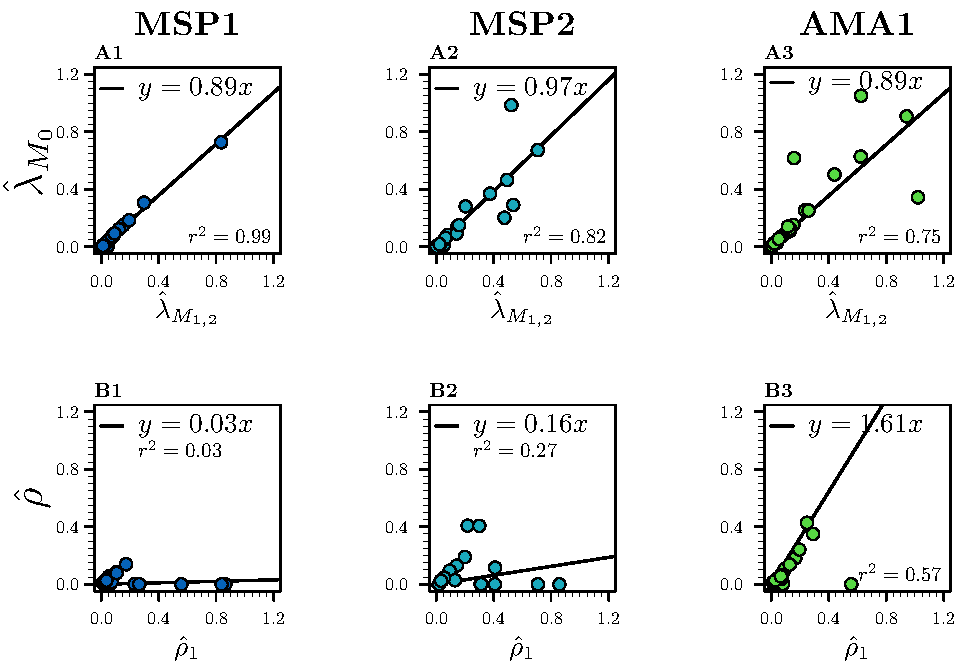
\includegraphics[width=\columnwidth]{images/M0vM12.pdf}
\end{adjustbox}
\caption[Correlation analyses between parameter estimates from M$_0$ and M$_ {1,2}$]{Comparison of parameter estimates from models M$_0$ and M$_{1,2}$. The first column, with figures \textbf{A1} and \textbf{B1}, represents analyses made for the MSP1 antigen data set, the second column, with figures \textbf{A2} and \textbf{B2}, represents analyses using the MSP2 antigen data, and third column, with figures \textbf{A3} and \textbf{B3}, represents analyses for the AMA1 antigen data set. Figures \textbf{A1}, \textbf{A2}, and \textbf{A3} in the first row, shows the 21 model M$_0$ SCR estimates, $ \widehat{\lambda}_{M_0}$, as function of the corresponding M$_{1,2}$ estimates. Figures \textbf{B1}, \textbf{B2}, and \textbf{B3} in the second row represent model M$_0$ SRR estimates, $ \widehat{\rho}$, as function of the M$_{1,2}$'s $ \widehat{\rho}_1$, calculated before the cutoff value $ \widehat{\uptau}$. For the second row, villages with $ \widehat{\rho}_1>10$ were excluded form the analysis. For each graph the line of tendency (in black) with respective formula and corresponding Pearson's correlation statistics, $r^2$, is shown.}
\label{fig:comparisons.M0.M12}
\end{figure}


%%%%% MSP1 %%%%%
\begin{sidewaystable}
\centering
\caption[Likelihood ratio test for comparing RCMs M$_0$ and M$_{1,2}$, MSP1 antigen data]{Comparison between models M$_0$ and M$_{1,2}$ using the likelihood ratio test. Data used from the immune responses to \textit{P. falciparum}-MSP1 antigen in samples from the 21 villages. Model M$_0$ assumes a constant SCR and SRR ($\lambda$ and $\rho$, respectively), while model M$_{1,2}$ assumes a constant SCR, $\lambda_1$ for ages $<\uptau$ and $\lambda_2=0$ otherwise. LogL refers to the log-likelihood function evaluated at the respective maximum likelihood estimates using profile likelihood method. P-value is associated with the log-likelihood ratio test comparing the nested model M$_0$ with M$_{1,2}$. Estimated 95\% confidence intervals including $>$10 suggest the model did not have sufficient information to accurately estimate the lower and upper limits. This event can be mostly seen at high altitude villages.}
\label{tab:M0.M12.msp1}
\begin{adjustbox}{width=\linewidth}
%%%%%%%%%%%%%%%%%%%%%%%%%%%
%%%%% MSP1 - M0 vs M12 %%%%
%%%%%%%%%%%%%%%%%%%%%%%%%%%
\begin{tabular}{llllllllclr} 
\toprule
\multicolumn{1}{c}{\multirow{2}{*}{Transect}} & \multicolumn{1}{c}{\multirow{2}{*}{Village}} & \multicolumn{3}{c}{Model M$_{0}$} & \multicolumn{1}{c}{} & \multicolumn{4}{c}{Model M$_{1,2}$} & \multicolumn{1}{c}{\multirow{2}{*}{p-value}}  \\ 
\cmidrule{3-5}\cmidrule{7-10}
\multicolumn{1}{c}{} & \multicolumn{1}{c}{} & \multicolumn{1}{c}{$\hat{\lambda}$ (95\% CI)} & \multicolumn{1}{c}{$\hat{\rho}$ (95\% CI)} & \multicolumn{1}{c}{logL} & \multicolumn{1}{c}{} & \multicolumn{1}{c}{$\hat{\lambda}$ (95\% CI)} & \multicolumn{1}{c}{$\hat{\rho}_1$ (95\% CI)} & \multicolumn{1}{c}{$\hat{\uptau}$} & \multicolumn{1}{c}{logL} & \multicolumn{1}{c}{} \\
\midrule
Rombo       & Mokala          & 0.014 (0.008, 0.030)   & 0.016 (0.000, 0.093)   & -45.68   & & 0.016 (0.009, $>$5)   & 0.031 (0.000, $>$10)   & 30 & -45.63 & 0.752\\
              & Machame Aleni & 0.047 (0.024, 0.140)   & 0.083 (0.020, 0.372)   & -56.54   & & 0.052 (0.027, $>$5)   & 0.104 (0.031, 0.460)   & 37 & -56.01 & 0.303\\
              & Ikuini        & 0.014 (0.010, 0.038)   & 0.000 (0.000, 0.102)   & -58.55   & & 0.020 (0.011, $>$5)   & 0.061 (0.000, $>$10)   & 22 & -58.16 & 0.377\\
              & Kileo         & 0.307 (0.205, 0.499)   & 0.055 (0.023, 0.125)   & -44.77   & & 0.298 (0.210, $>$5)   & 0.055 (0.026, 0.110)   & 40 & -45.61 & $\sim$1.000\\
\cmidrule{2-11}
N. Pare     & Kilomeni        & 0.005 (0.002, 0.038)   & 0.000 (0.000, 0.351)   & -18.93   & & 0.046 (0.004, $>$5)   & 0.864 (0.000, $>$10)   & 30 & -17.22 & 0.064\\
            & Lambo           & 0.015 (0.010, 0.041)   & 0.001 (0.000, 0.104)   & -37.86   & & 0.019 (0.010, $>$5)   & 0.232 (0.000, $>$10)   & 7  & -37.60 & 0.471\\
            & Ngulu           & 0.074 (0.046, 0.159)   & 0.000 (0.000, 0.058)   & -13.79   & & 0.084 (0.052, $>$5)   & $>$10 (0.000, $>$10)   & 1  & -13.31 & 0.327\\
            & Kambi ya Simba  & 0.067 (0.039, 0.122)   & 0.010 (0.000, 0.059)   & -27.45   & & 0.074 (0.043, $>$5)   & 0.019 (0.000, $>$10)   & 36 & -27.01 & 0.348\\
\cmidrule{2-11}
S. Pare     & Bwambo          & 0.005 (0.003, 0.017)   & 0.000 (0.000, 0.126)   & -36.14   & & 0.017 (0.004, $>$5)   & 0.265 (0.000, $>$10)   & 27 & -34.93 & 0.120\\
            & Mpinji          & 0.005 (0.002, 0.009)   & 0.000 (0.000, 0.055)   & -21.75   & & 0.009 (0.005, $>$5)   & $>$10 (0.134, $>$15)   & 8  & -19.23 & 0.025\\
            & Goha            & 0.032 (0.021, 0.054)   & 0.017 (0.000, 0.070)   & -58.55   & & 0.042 (0.025, $>$5)   & 0.073 (0.000, 0.196)   & 24 & -57.35 & 0.121\\
            & Kadando         & 0.152 (0.108, 0.230)   & 0.029 (0.011, 0.068)   & -57.05   & & 0.156 (0.115, $>$5)   & 0.032 (0.014, 0.069)   & 38 & -56.82 & 0.498\\
\cmidrule{2-11}
W. Usamb. 1 & Emmao           & 0.001 (0.000, 0.127)   & 0.000 (0.000, $>$10)   & -10.86   & & 0.006 (0.001, $>$5)   & 0.838 (0.000, $>$10)   & 26 &  -9.68 & 0.124\\
            & Handei          & 0.044 (0.021, 0.128)   & 0.139 (0.040, 0.520)   & -57.56   & & 0.049 (0.025, $>$5)   & 0.173 (0.062, 0.527)   & 37 & -56.42 & 0.131\\
            & Tewe            & 0.026 (0.020, 0.040)   & 0.000 (0.000, 0.032)   & -64.19   & & 0.030 (0.023, $>$5)   & $>$10 (0.000, $>$10)   & 2  & -62.63 & 0.077\\
            & Mn'galo         & 0.074 (0.056, 0.099)   & 0.009 (0.000, 0.026)   & -67.23   & & 0.075 (0.058, $>$5)   & 0.010 (0.000, $>$10)   & 40 & -67.08 & 0.584\\
\cmidrule{2-11}
W. Usamb. 2 & Kwadoe          & 0.007 (0.004, 0.011)   & 0.000 (0.000, 0.032)   & -37.52   & & 0.013 (0.007, $>$5)   & 0.558 (0.013, 2.794)   & 14 & -35.47 & 0.043\\
            & Funta           & 0.121 (0.088, 0.172)   & 0.018 (0.005, 0.045)   & -47.92   & & 0.123 (0.093, 0.169)  & 0.020 (0.007, 0.045)   & 40 & -47.46 & 0.337\\
            & Tamota          & 0.093 (0.063, 0.152)   & 0.041 (0.014, 0.100)   & -64.58   & & 0.092 (0.066, $>$5)   & 0.042 (0.017, 0.091)   & 40 & -65.06 & $\sim$1.000\\
            & Mgila           & 0.184 (0.131, 0.286)   & 0.026 (0.008, 0.070)   & -64.36   & & 0.194 (0.140, $>$5)   & 0.036 (0.013, 0.091)   & 33 & -64.45 & $\sim$1.000\\
\cmidrule{2-11}
W. Usamb. 3 & Mgome           & 0.727 (0.398, 4.520)   & 0.078 (0.023, 0.482)   & -34.25   & & 0.835 (0.457, $>$5)   & 0.107 (0.035, $>$10)   & 37 & -32.48 & 0.060\\
\bottomrule
\end{tabular}
\end{adjustbox}
\end{sidewaystable}

\newpage

%%%%% Figure %%%%%
\begin{figure}[H]
\center
\begin{adjustbox}{width=\linewidth,totalheight=\textheight-4\baselineskip}
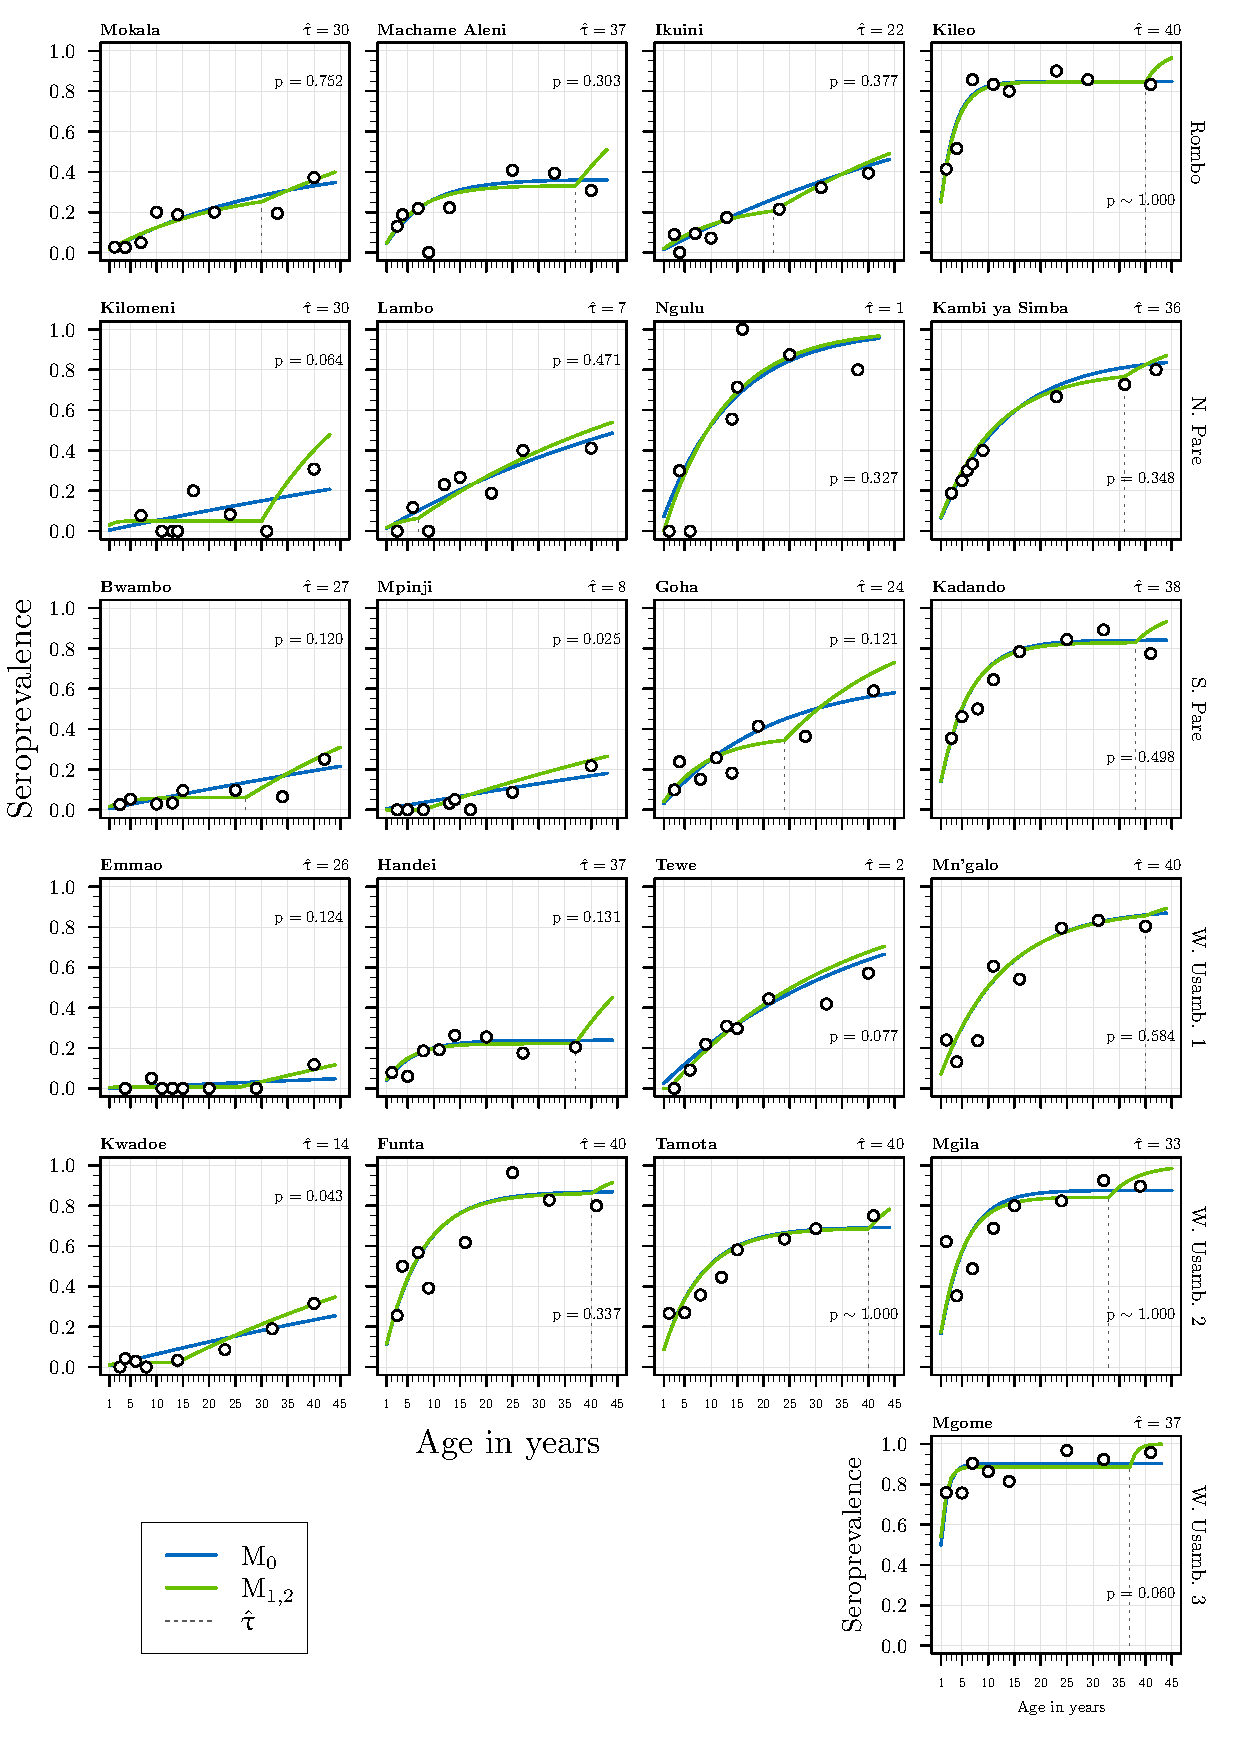
\includegraphics[width=\columnwidth]{images/Seroprevalence_M0vM12_msp1.pdf}
\end{adjustbox}
\caption[Estimated MSP1 seroprevalence for models M$_0$ and M$_{1,2}$]{Fits for the estimated MSP1 antigen seroprevalence for the 21 assessed villages, using models M$_0$ (blue lines) and M$_{1,2}$ (green lines), with the cutoff parameter of the latter signalled. Each row of graphs represents data from the transects (identified on the right hand side), where villages are ordered by decreasing altitude (and increasing malaria incidence). In the different plots, the dots represent the observed seroprevalence of distinct age groups by splitting the sampled age distribution into similar bins. P-values from the resulting likelihood ratio tests are identified.}
\label{fig:msp1.seroprevalence.M0.M12}
\end{figure}

\newpage


%%%%%%%%%%%
% M0 v M2 %
%%%%%%%%%%%
\subsection[Testing change in seroconversion rate]{Testing change in SCR: M$_{0}$ \textit{vs.} M$_{2}$}

% With the change in SRR statistically non significant,
With a possible change in SRR discarded for most villages, model M$_0$ was compared against M$_2$ to test if the SCR in each village was reasonably constant throughout the past years (Table \ref{tab:M0.M2.msp1} for MSP1, and from Appendices \ref{appendix:M0vM2}, Tables \ref{tab:M0.M12.msp2} and \ref{tab:M0.M12.ama1} for MSP2 and AMA1, respectively).
Model M$_2$ was developed assuming a change in SCR occurred some time before the sampling.
% Such cahange be originated from a successful campaign for prevention and control of the disease.
% The sudden change in SCR exposes individuals to a different intensity of malaria transmission.
% and adjust their immunological system accordingly.
Based on the frequency of antigens detected at different ages, model M$_2$ was able to estimate how long ago that change occurred, assuming $1\leq \widehat{\uptau}^*\leq40$.
% \textcolor{red}{, and how abrupt it was; isto aqui não faz sentido, a change pode ser positiva ou negativa}.

The estimated seroprevalence curves produced by this model suggested that a change in transmission might have occurred in various villages (Figure \ref{fig:seroprevalence.M0.M2} for the estimated seroprevalence from MSP1, and Figures \ref{fig:msp2.seroprevalence.M0.M2} and \ref{fig:ama1.seroprevalence.M0.M2} from Appendices \ref{appendix:M2.seroprev.msp2} and \ref{appendix:M2.seroprev.ama1}, respectively, for estimated seroprevalence from MSP2 and AMA1).
However, from the likelihood ratio tests, the apparently evident changes in SCR seen in model M$_2$ were in fact only statistically significant for a few villages.
% The different immunogenic antigens presented different villages where a significant change may have occurred.
Results from the MSP1 antigen identified a significant change in SCR in Kwadoe, Tamota, Mgila (all from transect West Usambara 2), and Mgome (West Usambara 3).
Estimates for Kwadoe ($ \widehat{\uptau}^*=30$) indicated the SCR reduction occurred approximately between 27 and 32 years before sampling (Figure \ref{fig:profile.kwadoe}).
The remaining three villages estimated the cutoff for change in SCR between one and two years ($ \widehat{\uptau}^*=1$).
For the MSP2 data set, villages Bwambo ($ \widehat{\uptau}^*=37$) and Mpinji ($ \widehat{\uptau}^*=1$) from the South Pare transect, and Funta ($ \widehat{\uptau}^*=6$) and Tamota ($ \widehat{\uptau}^*=1$), both from West Usambara 2, were identified.
In Bwambo, the SCR reduction took place between 35 and 39 years before the survey sampling.
Similar to the lower altitude villages identified using the previous antigen, the changes in Mpinji and, once again, in Tamota were estimated to approximately occur just one to two years before the data collection.
And in Tamota, a the gange in SCR occurred approximately six years before the study.
Likelihood ratio tests from the AMA1 antigen suggested that only individuals from the village Machame Aleni ($ \widehat{\uptau}^*=20$), from the transect Rombo, were exposed to a significant reduction in SCR during the last 40 years.
This change was estimated to happen approximately 20 years before sampling.



% As the more immunogenic, AMA1 is expected to be more easily detected at lower intensities of transmission, where other antigens might be significantly reduced.
% This sensitivity have resulted in less significant or noticeable changes in seroprevalence estimation.
% Non significant changes in SCR for AMA1 antigens have also been reported in \textit{P. vivax} analyses, under similar conditions \cite{cook2010using}.

% Despite the parametric restriction proposed for model M$_2$ ($\lambda_1\geq\lambda_2$), some villages where $\uptau^*$ was equal to one, estimated $\lambda_2$ with a higher value than $\lambda_1$.
% Although not intended, by occurring almost entirely on medium to low altitude villages, this event could grant some information about the sites.
% In those villages, children between one and two years old represented the interval where model M$_2$ identified the greatest change in SCR across all ages.
% % This event ($\uptau^*=1$) causes M$_2$ to estimate seroprevalence using only the upper bracket from equation (\ref{eq:rcm.reduction.scr}).
% The seroprevalence curves generated under this assumption ($\uptau^*=1$) did not present the characteristic biphasic behaviour from M$_2$ (Figure \ref{fig:seroprevalence.M0.M12}).
% An example was the village Tamota.
% Despite a statistically significant change in SCR for two antigens, with an estimated cutoff equal to one, its maximum likelihood estimators for $\lambda_2$ were higher than $\lambda_1$ in both occasions.
% This could also be malfunction from the package, due to the small amount of information available to perform more precise estimations at each year.

%%%%% MSP1 %%%%%
\begin{sidewaystable}
\centering
\caption[Likelihood ratio test for comparing RCMs M$_0$ and M$_{2}$, MSP1 antigen data]{Comparative analysis of the results from models  M$_{0}$ and M$_{2}$, referring all 21 villages, considering MSP1 individual status as the outcomes. Model M$_{0}$ assumes constant SCR ($\lambda$) and SRR ($\rho$) for all ages. Model M$_{2}$ also assumes constant SRR, and a change in SCR after the cutoff parameter, $\uptau^*$. logL refers to the log-likelihood function evaluated at the respective maximum likelihood estimates using the profile likelihood method. p-value is associated with the log-likelihood ratio test comparing both models.}
\label{tab:M0.M2.msp1}
\begin{adjustbox}{width=\linewidth}
%%%%%%%%%%%%%%%%%%%%%%%%%%
%%%%% MSP1 - M0 vs M2 %%%%
%%%%%%%%%%%%%%%%%%%%%%%%%%
\begin{tabular}{lllllllllclr}
\toprule
\multicolumn{1}{c}{\multirow{2}{*}{Transect}} & \multicolumn{1}{c}{\multirow{2}{*}{Village}} & \multicolumn{3}{c}{Model M$_0$} & \multicolumn{1}{c}{} & \multicolumn{5}{c}{Model M$_2$} & \multicolumn{1}{c}{\multirow{2}{*}{p-value}}  \\ 
\cmidrule{3-5}\cmidrule{7-11}
\multicolumn{1}{c}{} & \multicolumn{1}{c}{} & \multicolumn{1}{c}{$\hat{\lambda}$ (95\% CI)} & \multicolumn{1}{c}{$\hat{\rho}$ (95\% CI)} & \multicolumn{1}{c}{logL} & \multicolumn{1}{c}{} & \multicolumn{1}{c}{$\hat{\lambda}_1$ (95\% CI)} & \multicolumn{1}{c}{$\hat{\lambda}_2$ (95\% CI)} & \multicolumn{1}{c}{$\hat{\rho}$ (95\% CI)} & \multicolumn{1}{c}{$\hat{\uptau}^*$} & \multicolumn{1}{c}{logL} & \multicolumn{1}{c}{} \\ 
\midrule
Rombo       & Mokala         & 0.014 (0.008, 0.030)   & 0.016 (0.000, 0.093)   & -45.68   & &   100.664 (0.006, $>$10) & 0.012 (0.004, 0.031)   & 0.190 (0.000, 0.243)   & 8   & -44.43   & 0.287\\
            & Machame Aleni  & 0.047 (0.024, 0.140)   & 0.083 (0.020, 0.372)   & -56.54   & &   54.484 (0.000, $>$10)  & 0.045 (0.026, 0.085)   & 0.107 (0.031, 0.203)   & 14  & -55.23   & 0.270\\
            & Ikuini         & 0.014 (0.010, 0.038)   & 0.000 (0.000, 0.102)   & -58.55   & &   0.011 (0.006, 0.025)   & 0.051 (0.012, 0.116)   & 0.000 (0.000, 0.053)   & 1   & -56.88   & 0.188\\
            & Kileo          & 0.307 (0.205, 0.499)   & 0.055 (0.023, 0.125)   & -44.77   & &   236.197 (0.122, $>$10) & 0.287 (0.184, 0.449)   & 0.077 (0.031, 0.127)   & 4   & -43.83   & 0.391\\
\cmidrule{2-12}
N. Pare     & Kilomeni       & 0.005 (0.002, 0.038)   & 0.000 (0.000, 0.351)   & -18.93   & &   0.027 (0.000, $>$10)   & 0.004 (0.001, 0.013)   & 0.003 (0.000, 0.103)   & 27  & -17.84   & 0.336\\
            & Lambo          & 0.015 (0.010, 0.041)   & 0.001 (0.000, 0.104)   & -37.86   & &   78.671 (0.000, $>$10)  & 0.010 (0.002, 0.035)   & 0.125 (0.000, 0.180)   & 10  & -36.47   & 0.249\\
            & Ngulu          & 0.074 (0.046, 0.159)   & 0.000 (0.000, 0.058)   & -13.79   & &   58.997 (0.071, $>$10)  & 0.038 (0.009, 0.105)   & 0.018 (0.000, 0.046)   & 13  & -11.88   & 0.148\\
            & Kambi ya Simba & 0.067 (0.039, 0.122)   & 0.010 (0.000, 0.059)   & -27.45   & &   44.179 (0.000, $>$10)  & 0.068 (0.040, 0.112)   & 0.023 (0.000, 0.055)   & 17  & -27.02   & 0.651\\
\cmidrule{2-12}
S. Pare     & Bwambo         & 0.005 (0.003, 0.017)   & 0.000 (0.000, 0.126)   & -36.14   & &   20.786 (0.000, $>$10)  & 0.006 (0.003, 0.011)   & 0.039 (0.000, 0.070)   & 35  & -33.49   & 0.071\\
            & Mpinji         & 0.005 (0.002, 0.009)   & 0.000 (0.000, 0.055)   & -21.75   & &   1.962 (0.008, $>$10)   & 0.003 (0.001, 0.008)   & 0.058 (0.000, 0.092)   & 24  & -18.88   & 0.057\\
            & Goha           & 0.032 (0.021, 0.054)   & 0.017 (0.000, 0.070)   & -58.55   & &   0.019 (0.012, 0.036)   & 0.061 (0.029, 0.102)   & 0.000 (0.000, 0.034)   & 2   & -56.59   & 0.141\\
            & Kadando        & 0.152 (0.108, 0.230)   & 0.029 (0.011, 0.068)   & -57.05   & &   0.093 (0.046, 0.161)   & 0.343 (0.164, 0.575)   & 0.018 (0.000, 0.046)   & 1   & -54.54   & 0.081\\
\cmidrule{2-12}
W. Usamb. 1 & Emmao          & 0.001 (0.000, 0.127)   & 0.000 (0.000, $>$10)   & -10.86   & &   24.373 (0.000, $>$10)  & 0.001 (0.000, 0.005)   & 0.081 (0.000, 0.219)   & 30  & -9.35    & 0.221\\
            & Handei         & 0.044 (0.021, 0.128)   & 0.139 (0.040, 0.520)   & -57.56   & &   117.997 (0.000, $>$10) & 0.047 (0.022, 0.100)   & 0.282 (0.000, 0.434)   & 7   & -56.68   & 0.415\\
            & Tewe           & 0.026 (0.020, 0.040)   & 0.000 (0.000, 0.032)   & -64.19   & &   0.048 (0.026, 0.089)   & 0.000 (0.000, 0.022)   & 0.022 (0.000, 0.065)   & 3   & -61.72   & 0.085\\
            & Mn'galo        & 0.074 (0.056, 0.099)   & 0.009 (0.000, 0.026)   & -67.23   & &   50.536 (0.167, $>$10)  & 0.071 (0.054, 0.092)   & 0.022 (0.014, 0.034)   & 15  & -64.46   & 0.063\\
\cmidrule{2-12}
W. Usamb. 2 & Kwadoe         & 0.007 (0.004, 0.011)   & 0.000 (0.000, 0.032)   & -37.52   & &   2.652 (0.299, $>$10)   & 0.004 (0.002, 0.008)   & 0.038 (0.026, 0.056)   & 30  & -31.49   & 0.002\\
            & Funta          & 0.121 (0.088, 0.172)   & 0.018 (0.005, 0.045)   & -47.92   & &   59.081 (0.000, $>$10)  & 0.116 (0.087, 0.157)   & 0.022 (0.011, 0.042)   & 13  & -46.53   & 0.249\\
            & Tamota         & 0.093 (0.063, 0.152)   & 0.041 (0.014, 0.100)   & -64.58   & &   0.046 (0.023, 0.084)   & 0.243 (0.128, 0.389)   & 0.016 (0.000, 0.051)   & 1   & -60.30   & 0.014\\
            & Mgila          & 0.184 (0.131, 0.286)   & 0.026 (0.008, 0.070)   & -64.36   & &   0.062 (0.038, 0.110)   & 0.579 (0.378, 0.807)   & 0.002 (0.000, 0.023)   & 1   & -53.04   & $<$0.001\\
\cmidrule{2-12}
W. Usamb. 3 & Mgome          & 0.727 (0.398, 4.520)   & 0.078 (0.023, 0.482)   & -34.25   & &   0.088 (0.023, 0.432)   & 1.310 (0.748, 1.847)   & 0.010 (0.000, 0.088)   & 1   & -30.86   & 0.034\\
\bottomrule
\end{tabular}
\end{adjustbox}
\end{sidewaystable}

\newpage

%%%%% Figure %%%%%
\begin{figure}[H]
\center
\begin{adjustbox}{width=\linewidth,totalheight=\textheight-5\baselineskip}
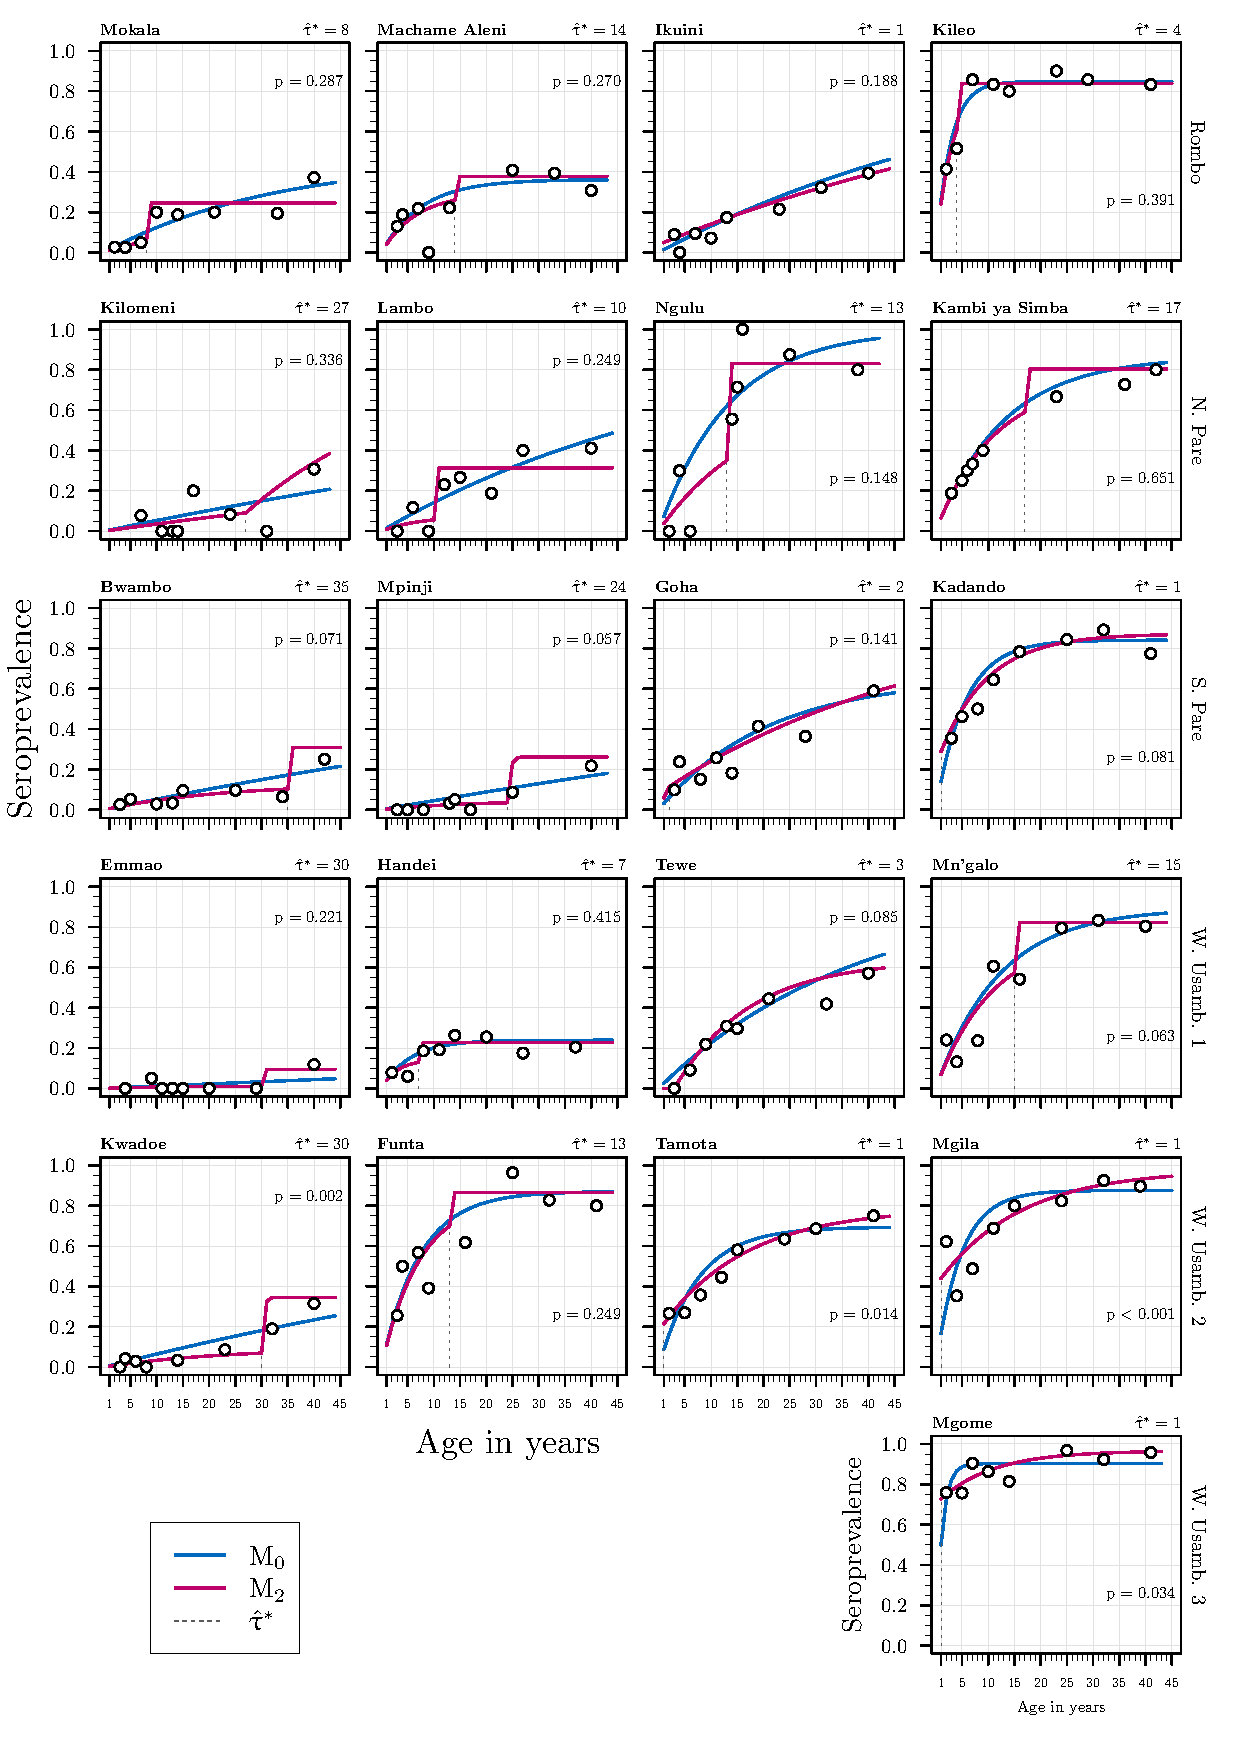
\includegraphics[width=\columnwidth]{images/Seroprevalence_M0vM2_msp1.pdf}
\end{adjustbox}
\caption[Estimated MSP1 seroprevalence for models M$_0$ and M$_2$]{Fits for the estimated MSP1 antigen seroprevalence for the 21 assessed villages, using models M$_0$ (blue lines) and M$_2$ (light red lines), with the cutoff parameter of the latter signalled, identifying the change in SCR happening in years before sampling. Each row of graphs represents data from the transects (identified on the right hand side), where villages are ordered by decreasing altitude (and increasing malaria incidence). In the different plots, the dots represent the observed seroprevalence of distinct age groups by splitting the sampled age distribution into similar bins. P-values from the resulting likelihood ratio tests are identified.}
\label{fig:seroprevalence.M0.M2}
\end{figure}


\begin{figure}[ht!]
\center
\begin{adjustbox}{width=\linewidth}
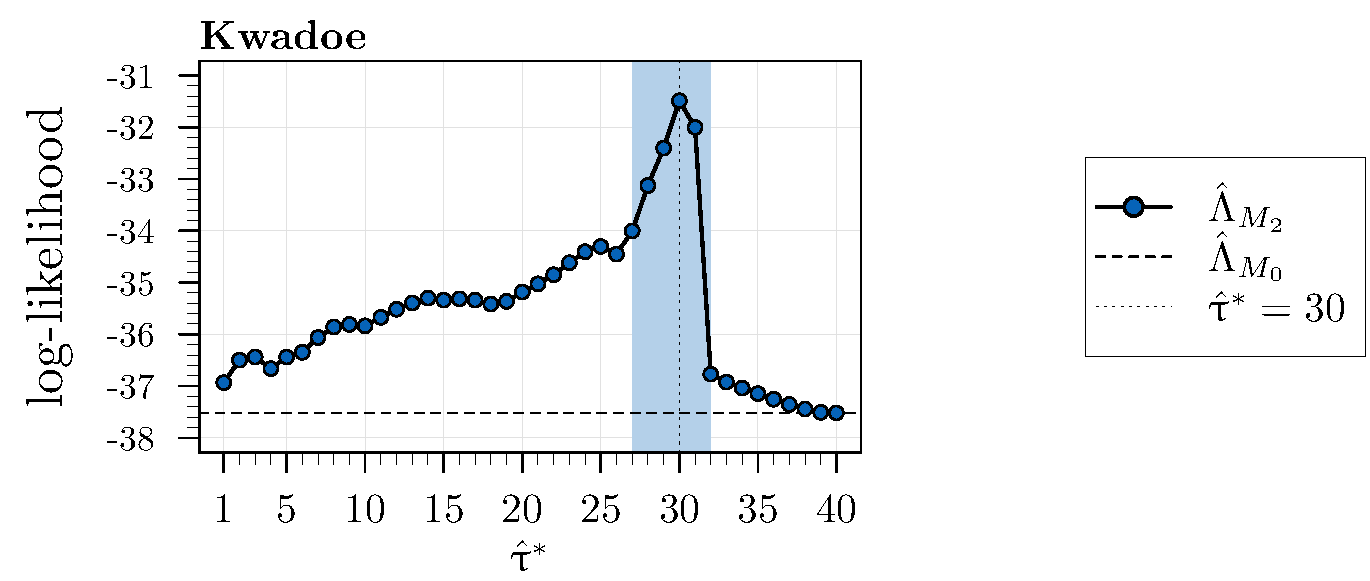
\includegraphics[width=\columnwidth]{images/profile_kwadoe.pdf}
\end{adjustbox}
\caption[Profile likelihood methodology for estimation of parameters from village Kwadoe, MSP1 antigen data]{Example of the profile likelihood methodology implemented to estimate parameter values from village Kwadoe in model M$_2$. Parameters that maximised the log-likelihood were estimated by gradually increasing one unit in the cutoff parameter $\uptau^*$ and estimate the remaining parameters $\lambda_1$, $\lambda_2$, and $\rho$ at each level, via maximum likelihood. Estimate $ \widehat{\uptau}^*=30$ (thin dashed line) returns the maximum value of log-likelihood and all the associated parameters. The Horizontal dashed line represents the maximum log-likelihood estimated using model M$_0$, under the same data set.}
\label{fig:profile.kwadoe}
\end{figure}

%%%%%%%%%%%%%
%% M12 v M2 %
%%%%%%%%%%%%%
%\subsubsection{M$_{2}$ \textit{vs} M$_{1,2}$}
%Tenho esta comparação. Are they nested? Is it worth it?
%Testing for evident changes in SRR and SCR by comparing models M$_{1,2}$ and M$_{2}$ against M$_{0}$ has shown that for most situations, the simpler model is the more parsimonious one.
%%%%%% MSP1 %%%%%
%\begin{sidewaystable}
%\centering
%\caption[Comparison of RCM models M$_{1,2}$ and M$_{2}$ applied to the MSP1 data set]{.}
%\label{tab:M12.M2.msp1}
%\begin{adjustbox}{width=\linewidth}
%\input{tables/table_M12vM2_msp1.tex}
%\end{adjustbox}
%\end{sidewaystable}
%
%%%%%% MSP2 %%%%%
%\begin{sidewaystable}
%\centering
%\caption[Comparison of RCM models M$_{1,2}$ and M$_{2}$ applied to the MSP2 data set]{Statistical analysis of the MSP2 antigen data set referring to the 21 Tanzanian villages.}
%\label{tab:M12.M2.msp2}
%\begin{adjustbox}{width=\linewidth}
%\input{tables/table_M12vM2_msp2.tex}
%\end{adjustbox}
%\end{sidewaystable}
%
%%%%%% AMA1 %%%%%
%\begin{sidewaystable}
%\centering
%\caption[Comparison of RCM models M$_{1,2}$ and M$_{2}$ applied to the AMA1 data set]{Statistical analysis of the AMA1 antigen data set referring to the 21 Tanzanian villages.}
%\label{tab:M12.M2.ama1}
%\begin{adjustbox}{width=\linewidth}
%\input{tables/table_M12vM2_ama1.tex}
%\end{adjustbox}
%\end{sidewaystable}

\section{Antibody seroprevalence as indicator of malaria transmission intensity}
% \textcolor{red}{E agora o que é que acontece à transmissão actual em cada uma das vilas? Como varia? What about interpretations about SCR for all villages? Pelo menos um parágrafo a explicar a transmissão! Meter a figura que enviei, analisar! Análise final: qual é a corelação entre prevalência de infecção e seroprevalence!!
% Devia mostrar prof likelihood para as vilas em que há uma redução significativa.}
% (Table \ref{tab:EIR.to.SCR} from Appendices)
% When assessing how malaria transmission rate behaves across the studied villages, the serology-based models characterise the populations' current state of transmission intensity by focusing on the presence/absence of specific malarial antigens.
% The RCMs went even further, describing how transmission intensity evolved across the sequence of ages, translating the estimated rates into age-specific seroprevalence values for each site.

With the more parsimonious serology-based model for each one of the studied villages identified, inferences about possible patterns in transmission intensity and how the seroprevalence evolved over time were performed.
Irrespective of the malarial antigen analysed, most villages were best described considering SCR and SRR as constant transition rates across all ages (model M$_0$).
An overall analysis on the model estimates implied a noticeable influence of altitude on the SCR, proxy for transmission intensity (Figure \ref{fig:M0.SCR.altitude}).
As seen when describing the age-dependent model M$_{1,2}$, SCR estimates suggested an inverse relation with altitude.
Similarly, the different $ \widehat{\lambda}$ estimates from M$_0$ presented moderate correlation with altitude ($r^2_{MSP1}=0.46$, $r^2_{MSP2}=0.42$, and $r^2_{AMA1}=0.48$).
The analysis between the estimates produced with different antigens corroborated a conclusion made in Chapter \ref{ch:4.0}, indicating AMA1 as the most immunogenic antigen of the three.
The SCR estimated when using the serological data for this antigen were consistently higher across all villages, when compared to the remaining antigens.
Meaning that even at high altitudes (lower transmission intensities), some levels of AMA1 antigens could be more easily detected in the individual's blood stream.
The results suggested MSP1 to be the less immunogenic, confirming the results observed during the exploratory analysis (Table \ref{tab:prevalence.seroprevalence} from Chapter \ref{ch:2.0}).

\begin{figure}[ht!]
\center
\begin{adjustbox}{width=\linewidth}
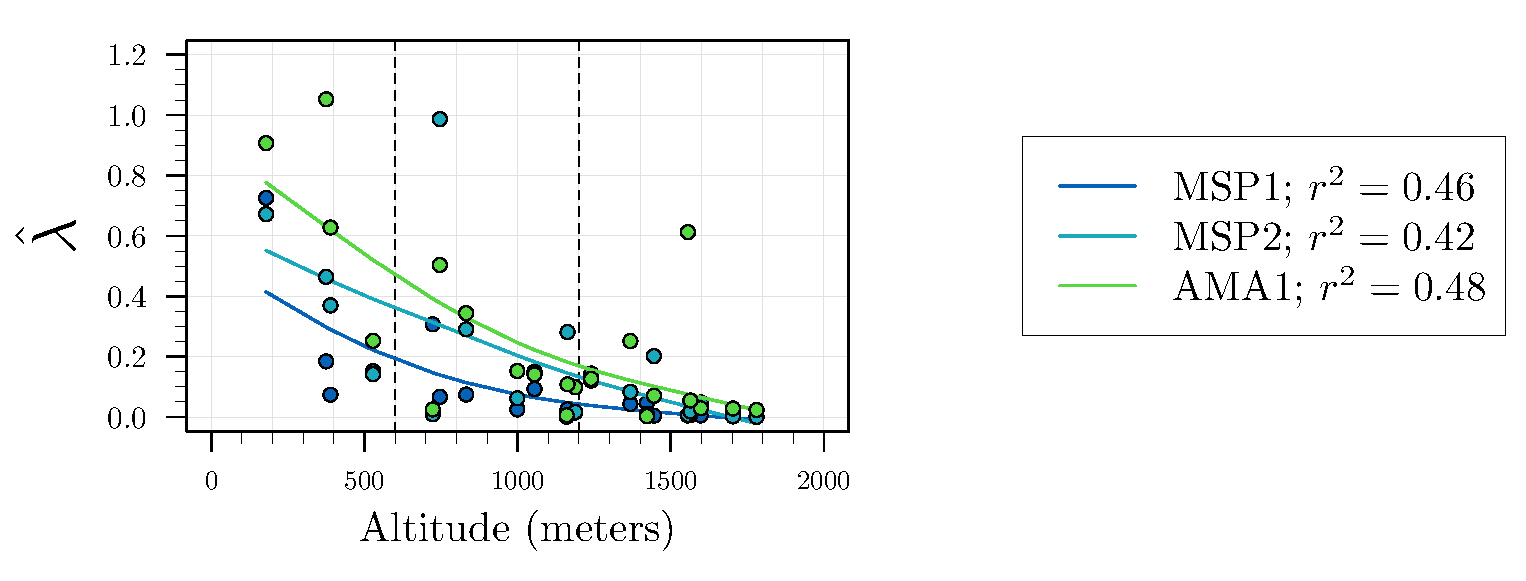
\includegraphics[width=\columnwidth]{images/M0_vs_altitude.pdf}
\end{adjustbox}
\caption[Dependency between altitude and SCR estimates]{Estimated SCR for each village using the RCM M$_0$. Each coloured point represents the transmission intensity estimated for each antigen data (MSP1, MSP2, and AMA1), as function of the respective village's altitude. The coloured lines are but an emphatic description of the transmission's trend. Vertical dashed lines represent the defined altitude limits, distinguishing between high ($>$1200m), medium (600m$-$1200m) and low ($<$600m) altitude villages.}
\label{fig:M0.SCR.altitude}
\end{figure}

Focusing on different transects encompassing clusters of altitude-defined villages, as well as some population genetic traits, transects from the Tanga region (West Usambara 1, 2, and 3) suggested higher estimated levels of transmission intensity.
More often villages from this region experienced a significant change in SCR some time before the sampling collection.
West Usambara 2 and West Usambara 3 (village Mgome), had their current estimates for SCR ($ \widehat{\lambda}$ or $ \widehat{\lambda}_2$, depending on the selected model) generally above $0.100$ in all data sets.
Transects from the Kilimanjaro region (transects Rombo, North, and South Pare) suggested lower estimates for transmission intensity.
Despite having similar structures in altitude, when compared to the villages from Tanga, the Kilimanjaro transects were located more inland, where a lesser humid climate is expected and could have presented an influence on the \textit{Anopheles} mosquitoes capacity.
The estimated values from Rombo relatively to the MSP1 data could suggest some affinity from individuals of the Wachaga ethnic group to produce the specific antibodies for the antigen.
The transmission intensities estimated in villages from this transect were notoriously higher, presenting similar levels to villages with higher measures of prevalence of infection.
However, the there was no strong discernible differences other than altitude and its effects on climate, that could indicate the reason for the different transmission intensities estimated.

%%%%%%%%%%%
% SUMMARY %
%%%%%%%%%%%
\section{Summary}

Comparing different nested RCMs to test biological and epidemiological hypotheses came to show that although seemingly close to a more realistic scenario, the effects of acquired immunity (model M$_{1,2}$), or past impacts from possible control measures (model M$_2$), did not present an impactful statistically significance, when applied to the data.
Model M$_0$ significantly described most of the studied villages.
Some exceptions were the villages Tamota and Mgila, best described by the RCM M$_2$, estimating that a recent change in SCR had occurred in the past years.
Model M$_{1,2}$ was also significant for some sites, describing villages located at intermediate and higher altitudes, such as Mpinji and Goha from the South Pare transect.

Correlation studies between M$_{1,2}$ and the more parsimonious M$_0$ suggested that neglecting to consider the age-dependent immunological uplift creates major underestimations in the SRR estimates, when considering the antigens MSP1 and MSP2.
% % Despite some villages evidencing a significant change in SCR, the overall best, model M$_0$, assumed both transition rates to be constant across all ages.
% The epidemiological proposal for past impacts able to effectively produce changes in malaria transmission was also dismissed for most villages.
% % Results based on this inference, modelled by M$_2$, were statistically non significant for the AMA1 data, with few villages from the MSP1$_{1,2}$ and MSP2 data sets deemed viable, when compared against M$_0$.
The simpler model M$_0$, with generally higher log-likelihoods than the remaining, more complex RCMs, is then considered the best model for the analysed data.
This conclusion implies that a more generalist model will prevail over other, more specialised proposals, when the population sample sizes under analysis do not provide sufficient data that would allow better estimations of parameters from the different models.
Results obtained by model M$_0$ demonstrated the dependency between the annual rate of seroconversion and altitude, with estimates for the AMA1 antigen being consistently higher than the others.
% \textcolor{red}{ tau^*==1 pode ser efeito dos maternal antibodies olhando figura 5.2. parece que o cutoff de idade de 1 ano poderá não ser o melhor cutoff Poderia ver a prevalência de infecção nos indivíduos com 1 ano de idade}.
% \textcolor{red}{TENHO DE POR CHAPÉU EM TODOS OS PARÂMETROS!!!!}
% Being the statistically more parsimonious, model M$_0$ presented underestimated parameter values when compared to M$_{1,2}$.
% It is worth mention the estimation of SRR has been shown difficult to estimate when using cross-sectional surveys.
% The difficulty can create some uncertainties when estimating the change point parameter $\uptau$, in the profile likelihood method.
% Are examples the model results for the MSP1 seroprevalence outcome (Table \ref{tab:M12.M11.msp1}), where both models estimate $\rho_1$ equal to zero at different cutoff values, for the villages Kilomeni, Ngulu, Mpinji, Tewe, and Kwadoe.
% As the more immunogenic, AMA1 is expected to be more easily detected at lower intensities of transmission, where other antigens might be significantly reduced.
% This sensitivity have resulted in less significant or noticeable changes in seroprevalence estimation.
% Non significant changes in SCR for AMA1 antigens have also been reported in \textit{P. vivax} analyses, under similar conditions \cite{cook2010using}.

% Despite the parametric restriction proposed for model M$_2$ ($\lambda_1\geq\lambda_2$), some villages where $\uptau^*$ was equal to one, estimated $\lambda_2$ with a higher value than $\lambda_1$.
% Although not intended, by occurring almost entirely on medium to low altitude villages, this event could grant some information about the sites.
% In those villages, children between one and two years old represented the interval where model M$_2$ identified the greatest change in SCR across all ages.
% % This event ($\uptau^*=1$) causes M$_2$ to estimate seroprevalence using only the upper bracket from equation (\ref{eq:rcm.reduction.scr}).
% The seroprevalence curves generated under this assumption ($\uptau^*=1$) did not present the characteristic biphasic behaviour from M$_2$ (Figure \ref{fig:seroprevalence.M0.M12}).
% An example was the village Tamota.
% Despite a statistically significant change in SCR for two antigens, with an estimated cutoff equal to one, its maximum likelihood estimators for $\lambda_2$ were higher than $\lambda_1$ in both occasions.
% This could also be malfunction from the package, due to the small amount of information available to perform more precise estimations at each year.


%%%%%%%%%%%%%%%%%%%%%%
%%%%% DISCUSSION %%%%%
%%%%%%%%%%%%%%%%%%%%%%
%%%%%%%%%%%%%%%%%%%%%%%%%%
%%%%%   DISCUSSION   %%%%%
%%%%%%%%%%%%%%%%%%%%%%%%%%
\chapter{Discussion}
\label{ch:discussion}

%%%%%%%%%%%%
% OVERVIEW %
%%%%%%%%%%%%
\section{Project overview}

% \textcolor{red}{Falar em como GMLs dizem que etnia Wachaga tem 1.81 de risco de ser infectado, mas que na realidade esse grupo é o menos afectado de todos. Possivelmente porque Others e Wachaga teriam que estar nas mesmas condições e os primeiros estão muito menos preparados para lidar com qualquer tipo de prevalência?}

% \textcolor{red}{Different statistical approaches can be applied when studying malaria transmission intensity.Knowing how to apply different methodologies and models is crucial when evaluating or developing projects for public health interventions, or plan for possible infectious disease outbreaks \cite{keeling2009mathematical}}.
% \textcolor{red}{Colocar parágrafos mais curtos.}
The main objective of this project was to estimate and describe malaria transmission intensity, assessing the heterogeneity values from different sites.
Using a benchmark cross-sectional survey data set from 21 Northeast Tanzanian villages with different endemic malaria intensities, various statistical methods were applied and tested.
First, based on the recorded infections amongst individuals from the different population cohorts, generalised linear models (GLMs) were built (Chapter \ref{ch:4.0}).
The models were set to infer about the primary transmission determinants influencing prevalence of infection.
% The infection status from the sampled individuals was used as outcome when assessing the primary risk factors for infection incidence.
Using different comparison methods and goodness-of-fit test statistics, the best model was selected.
This structure when applied to a model described prevalence of infection through significant determinants such as altitude, transect, ethnic, gender, age groups, and the presence of antibodies for malaria antigens.
Associating variables altitude and age group was also important to recreate a simplified categorical prevalence peak-shift, typically noticed when studying malaria in age-defined populations.
% The study of exposure factors was of importance to identify and predict how malaria was expected develop at different villages \cite{binka1995risk}.
The relative influence each demographical and exposure determinant had on prevalence of infection was assessed by the analyses of the model's odds ratios.
The results corroborated what previous literature had described, relating altitude as proxy for malaria transmission intensity \cite{drakeley2005altitude, bodker2003relationship}, and identifying the importance of individual characteristic, such as age group \cite{carneiro2010age} or ethnicity (genetic background), when inferring about risk of \textit{P. falciparum} malaria infection.
% granting individual protection \textcolor{red}{não trabalhei com protecção!! Não é necessário colocar isto, não vale a pena}.
% This tool can be used to predict possible hotspots of infection.
% Measures such as the prevalence rate or the entomological inoculation rate usually provide support to such inferences \cite{}.
Results shown by the three exposure antigens \textit{MSP1}, \textit{MSP2}, and \textit{AMA1} suggested that their presence consistently increased the odds of infection, thus evidencing their importance as immunological and hazard indicators as a consequence to the exposure to \textit{P. falciparum} parasites.
For the most immunogenic case, the sheer presence of the AMA1 antigen detected in children living in Mgome -- the most vulnerable age group and the village with the highest registered prevalence, 50.67\% -- increased the odds of infection from 61\% up to 136\%.
This sensitivity for the exposure antigens to indicate individuals at odds based on their serological status was then used to measure the exposure to malaria parasites.
% provided by the immunological variables was used.

With some of the studied villages in a state of malaria pre-elimination -- potentially presenting recurrent asymptomatic cases -- the use of exposure antigens could bring information to more accurately measure malaria transmission intensity.
Using the serological status for the three antigens as outcome of interest, reverse catalytic models (RCMs) were applied, assuming age as a proxy for time of exposure (Chapter \ref{ch:5.0}).
% To optimise the study effectiveness to measure transmission intensity on those sites, reverse catalytic models (RCMs) were applied.
Under different biological and epidemiological viewpoints, distinct RCMs were used.
Their sero-epidemiological results were compared, characterising the transmission intensity from each village.
% In these scenarios the more widely used case detection tools become limited to effectively estimate malaria transmission intensity \cite{stresman2012malaria}.
% Once this low infection rate threshold is reached, clear malaria symptomatic cases become rare.
% Even if mild symptoms were to be present, individuals might not seek for aid, as the disease it is not their main awareness concern \cite{}.
% If they do, the infection can be misdiagnosed for other more common diseases at the time \cite{}.
% Also, when inhabitants do not fear the impact of the low and controlled disease manifestations, areas with negligible transmission intensity may become challenges to reach an effective sample size and granting an adequate study power \cite{}.
% %To deal with the  key approach to optimizing malaria responses within a country will be structuring programmes in response to stratification by malaria burden and based on an analysis of past malaria incidence data, risk determinants related to the human host, parasites, vectors and the environment that together with an analysis of access to services..
% %The standard approaches are useful to estimate presence of infection in situations where endemic malaria occurs at high intensity rates, with several symptomatic cases at a time.
% %It is then necessary to study possible alternatives \cite{malera2011research} in order to optimise population screenings \cite{sachs2002economic, stewart2009rapid}.
% %as they tend to be expensive, time-consuming, and even with some lack of precision \cite{sachs2002economic, stewart2009rapid}.
Based on the data sets, the majority of the villages transmission intensity was better characterised by the simpler RCM M$_0$.
Estimates from this model, assuming both seroconversion and seroreversion rates (SCR and SRR) as constant across all ages, described the relations between transmission intensity and altitude, with SCR, proxy for transmission intensity, decreasing with altitude.
The results also showed how SRR was affected by the transmission intensity levels, reaching values close to zero in response to low estimates of SCR.
This might be due to the fact that in low transmission intensity villages, the transition into a antigen seropositive state tends to becomes a rare event.
With few seropositive individuals, the rate for seroreversion and antibody waning is expected to be close to non existent.

%%%%%%%%%%%%%%%%%%%%%%%%%%%%%%%
% IMPLICATIONS OF THE RESULTS %
%%%%%%%%%%%%%%%%%%%%%%%%%%%%%%%
\section{Epidemiological implications of the results}

% From the RCMs serological results, various conclusions can be taken.
% In the first comparison between the proposed age-dependent seroreversion rate (SRR) models, M$_{1,2}$ was selected as the more parsimonious model.
% The identification of this model suggested that after some time being exposed to a stable rate of transmission, all individuals, sooner or later, became permanently seropositives.
Recently, sero-epidemiological studies from longitudinal surveys have shown that some malaria antigens express a decrease in SRR with age \cite{ondigo2014estimation}. % QUENIA!!
These results came to contradict the overall assumption of constant SRR across all ages (assumed by the already published models M$_0$ and M$_2$).
This age-dependent SRR reduction was proposed in model M$_{1,2}$, with limited success in intermediate altitude villages, but mostly rejected for the simpler model M$_0$ regardless the antigens tested.
The results suggested that although biologically plausible, there was no sufficient information granted from the data that would allow the statistical acceptance of M$_{1,2}$.
% Under the analysed data, the seroprevalence estimates from both models were similar across all sites.
However, correlation tests showed underestimation of SCR from model M$_0$, relative to M$_{1,2}$.
Estimates for SRR were different depending on the antigen, although values of $ \widehat{\rho}_1$ could be tendentiously higher to compensate for the sudden decrease to $\rho_2=0$, given $ \widehat{\uptau}$.

The comparison of SCR estimates showed good correlations.
However, the small underestimations from M$_{0}$ (3\% to 11\% depending on the antigen) could become consequential in a scenario of low transmission settings, where accuracy is of most importance.
Estimates for SCR are usually the focused results when assessing malaria transmission intensity.
This rate can be representative of the force of infection \cite{hens2012modeling}, and its values have a clear transitional interpretation to more traditional measures, such as the entomological inoculation rate (Table \ref{tab:EIR.to.SCR} from Appendices) \cite{bodker2003relationship,drakeley2005estimating}.
With more areas reaching low transmission intensity, underestimating seroprevalence could produce misleading information, or even originate false sense of stability under a low transmission rate that otherwise could be taken for a somewhat more alarming event.
% A precise estimate of SRR at given time can also help to predict how the the serological status of a population is trending, allowing to develop and predict future actions accordingly.

Model M$_2$ was also used to estimate heterogeneity in malaria transmission.
Since its proposal, M$_2$ has been used as a complement to M$_0$ \cite{dewasurendra2017effectiveness} and applied to estimate and monitor the effectiveness of campaigns for malaria control \cite{cook2010using,cook2011serological}.
No literature was found indicating that specific actions for control of malaria infection took place on the studied villages.
% \textcolor{red}{In the Northeast Tanzanian case, neither the past serological status of each village, nor possible recent actions for control of malaria infections were known \textcolor{red}{unknown for you...}. Não existem artigos publicados na literatura que indiquem um controlo específico nestas populações.}
Model M$_2$ was then applied under the hypothesis of possible historical changes in transmission intensity, being tested against M$_0$ for the significance of such changes.
% under the epidemiological hypothesis that some villages could had in fact been exposed to interventions.
The comparison results suggested only few villages went through statistically significant SCR changes in past decades, and consequentially, their transmission intensity.
Other results suggested some villages had only recently changed their exposure rate (villages where $ \widehat{\uptau}^*=1$), consequently changing its SCR.
These sites were mostly located at low altitudes, with medium to high transmission settings.
% Despite the parametric restriction proposed for model M$_2$ ($\lambda_1\geq\lambda_2$), some villages where $\uptau^*$ was equal to one, estimated $\lambda_2$ with a higher value than $\lambda_1$.
% Although not intended, by occurring almost entirely on medium to low altitude villages, this event could grant some information about the sites.
% In those villages, children between one and two years old represented the interval where model M$_2$ identified the greatest change in SCR across all ages.
% % This event ($\uptau^*=1$) causes M$_2$ to estimate seroprevalence using only the upper bracket from equation (\ref{eq:rcm.reduction.scr}).
% The seroprevalence curves generated under this assumption ($\uptau^*=1$) did not present the characteristic biphasic behaviour from M$_2$ (Figure \ref{fig:seroprevalence.M0.M12}).
% An example was the village Tamota.
% Despite a statistically significant change in SCR for two antigens, with an estimated cutoff equal to one, its maximum likelihood estimators for $\lambda_2$ were higher than $\lambda_1$ in both occasions.
% This could also be malfunction from the package, due to the small amount of information available to perform more precise estimations at each year.
% Being the statistically more parsimonious, model M$_0$ presented underestimated parameter values when compared to M$_{1,2}$.
% It is worth mention the estimation of SRR has been shown difficult to estimate when using cross-sectional surveys.
% The difficulty can create some uncertainties when estimating the change point parameter $\uptau$, in the profile likelihood method.
% Are examples the model results for the MSP1 seroprevalence outcome (Table \ref{tab:M12.M11.msp1}), where both models estimate $\rho_1$ equal to zero at different cutoff values, for the villages Kilomeni, Ngulu, Mpinji, Tewe, and Kwadoe.
% As the more immunogenic, AMA1 is expected to be more easily detected at lower intensities of transmission, where other antigens might be significantly reduced.
% This sensitivity have resulted in less significant or noticeable changes in seroprevalence estimation.
% Non significant changes in SCR for AMA1 antigens have also been reported in \textit{P. vivax} analyses, under similar conditions \cite{cook2010using}.
For these situations, the parametric restriction proposed for model M$_2$ ($\lambda_1\geq\lambda_2$) was even disregarded, with estimates for $ \widehat{\lambda}_2$ presenting higher values than $ \widehat{\lambda}_1$.
One interpretation could be the detection of maternal antibodies that endured for more than the first year of a child's life.
Other hypothesis could be that with a widespread infection across all ages in low altitude villages, children between one and two years old represented the interval where model M$_2$ identified the more considerable change in SCR, representing when the infants first experiment an exposure to the malaria parasites.
Under this assumption of early SCR change, the generated seroprevalence curves did not present the characteristic biphasic behaviour (as seen in Figure \ref{fig:seroprevalence.M0.M2}).
% These estimates could also be a malfunction from the \emph{SEROAID} package, due to the reduced information available from the data to perform more precise estimations in each year.

The reduced number of significant changes in SCR when AMA1 antigen outcomes were used -- only one village identified -- have been reported in analyses done in \textit{P. vivax} parasites \cite{cook2010using}.
Due to its high immunogenicity (population reports for more than 80\% seropositive individuals by 20 years old \cite{ondigo2014estimation}), it is possible that despite an historical change, some molecular specialised tests still detected reasonable amounts of this antigen.



%%%%%%%%%%%%%%%
% LIMITATIONS %
%%%%%%%%%%%%%%%
\section{Statistical and epidemiological limitations}

% \textcolor{red}{variáveis climáticas estão diractamente relacionadas e representadas pela altitude.}
% During this project, important limitations were identified.
% First, the cross-sectional survey that originated the data.
% % used in a study pushing sero-epidemiology as a benchmark tool to estimate malaria transmission intensity in low transmission settings.
% The restricted sampling applied to the different population cohorts may have forced some level of heterogeneity amongst the individuals.
% To create similar transects of four distinct villages, the study may have forcibly encompassed geographically different villages.
% Transects such as Rombo or West Usambara 3 enclose distant villages.
% Contrarily, the South Pare transect selected villages with such high levels of proximity that they may influence each other.
% \textcolor{red}{Isto está errado -- cada transect tem um grupo específico!!!!}
% The identification of a major ethnic group describing each transect could have also originated biased interpretations based on genetic differences.
% Second, known important recorded variables were set aside for the study analyses.
% Climate characteristics such as temperature and rainfall, greatly influence transmission intensity through humidity and seasonality \cite{warrell2002essential, drakeley2005altitude}.
% With a set of villages defined by their altitude and geographical position, not including these explanatory variables must had greatly decreased the predictive power of the GLMs developed.

During this project, important limitations were identified.
The first was during the implementation of the simple GLMs to the data, when apparent more complex dependencies between variables were noticeable.
Within each transect, villages shared not only the same ethnic group, but also the described geographical proximity when in relation to the other studied sites.
When using the GLMs, these implications were disregarded with models assuming independence between the parameters of all villages.
The logistic \texttt{fit10} selected in Chapter \ref{ch:4.0}, performed well when inferring the odds of malaria infection, as well as justifying the heterogeneity measured.
% \textcolor{red}{However, despite the comparison methods suggesting good accuracy, uncertainties associated with the goodness-of-fit tests suggested some lack of information.}
The model was used for its descriptive abilities, being refrained from use as a broad predictive tool due to this limitation that could, eventually, be amended by focusing on the dependencies between variables.
% Dizer que, apesar de tudo, e embora os métodos de comparação tenham indicado boa precisão em relação ao modelo construído, os resultados do programa foram demonstrados como uma falha de informação, mantendo o modelo fit10 longe de ser perfeito. Este modelo não pode ser usado como uma ferramenta de previsão (ou seria suspeito).
These relations could possibly have been taken into account through use of generalised linear multilevel models (GLMMs).
The GLMMs delineate different hierarchical levels where the villages' systematic structures would be nested within a random factor level that could be defined by the transect categorical variable, \textit{Transect}.
However, the development of these more models was out of the scope of this thesis.
% would be time consuming, being set aside as the application and inference from the RCMs was the major purpose of the project.
% Although these correlations show how useful this set can be, the results do not go all the way when it comes to study the disease in low transmission settings \cite{stresman2012malaria}, thus application of alternative or more specific stochastic models to study disease spread can be a good alternative.

The RCMs also presented limitations as they are infinite population models.
% This set of models is specific for infinite populations.
Despite producing informative estimates, the application of the models to the limited sample sizes recorded in each village might not have been enough to statistically discern between each proposed model.
% \textcolor{red}{Não sabendo a village sample size posso estar muito longe da hipótese de infinite population}
Furthermore, the data in which the RCMs were applied to had a specific age structure with children between 1 and 4 years being oversampled in relation to other ages, because the original study used the effect of defined age groups in its survey \cite{drakeley2005estimating}.
Possibly, by increasing the sample size of the study, model M$_{1,2}$ would have a justification to be applied and produce more consistent significant results.
% Despite the global pattern justification form the models, by analysing the true prevalence values calculated at each village (Table \ref{tab:prevalence.seroprevalence}), one may see the predicted prevalence may have more 
% Also the recent signals for climate change and global warming may allow the \textit{Anopheles} mosquitoes to colonise higher altitudes and farther latitudes.
% Drug, sprays, and nets, although immensely useful in protecting the majority of the population and controlling infection spread, may never the part of the solution.
% Falar de vacinas!
% Vaccines exist for bacteria and viruses, who by comparison are simpler organisms.
% Referir a importância de criar unidades multidisciplinares para a actuação e eliminação da malária.
% Referiri de como um follow up study poderia evidenciar possíveis efeitos de migração/emigração dentro (e entre) as várias regiões.
% Seroepidemiological studies are especially useful in low transmission settings where the sensitivity of parasite prevalence surveys is limited by the scarcity of parasite positive individuals \cite{cook2010using}.
% Falar da temperatura e rainfall (importantes no estudo original) que têm grande efeito mas que não usei aqui -- pelo menos não directamente (usei altitude, que está correlacionada, justificar).
When applying this model, some villages certainly presented limited information to accurately estimate SRR (Tables \ref{tab:M0.M12.msp1} and Tables \ref{tab:M0.M12.msp2} and \ref{tab:M0.M12.ama1} from Appendices \ref{appendix:M0vM12}).
These situations resulted in non expected estimated values of $ \widehat{\rho}_1$ and respective confidence intervals, showing the difficulty of estimating the parameter when using samples form cross-sectional surveys.
The difficulty can also create some uncertainties when estimating the change point parameter $ \widehat{\uptau}$ in the profile likelihood method.
% However, if in further analyses this event continues to show, one could apply the data using a RCM under the complementary log-log equation (\ref{eq:rcm.cloglog}).

% \textcolor{red}{no caso de transição baixa rho~0, não é tao descabido assumir um modelo cloglog}
% \textcolor{red}{iSTO ESTÁ EM PORTUGUÊS: Are examples the model results for the MSP1 seroprevalence outcome (Table \ref{tab:M12.M11.msp1}), where both models estimate $\rho_1$ equal to zero at different cutoff values, for the villages Kilomeni, Ngulu, Mpinji, Tewe, and Kwadoe.}
% It is worth mention the estimation of SRR has been shown difficult to estimate when using cross-sectional surveys.
% This difficulty also created uncertainties when estimating the change point parameter $\uptau$ in the profile likelihood method.
% Are examples the model results for the MSP1 seroprevalence outcome (Table \ref{tab:M12.M11.msp1}), where both models estimate $\rho_1$ equal to zero at different cutoff values, for the villages Kilomeni, Ngulu, Mpinji, Tewe, and Kwadoe.
%However, the uncertainty association with the estimation of  is very high, as demonstrated by the respective confidence intervals. Note that data from Kilomeni and Tewe led to estimates of 1 equal to zero, showing the difficulty of estimating SRR using cross-sectional surveys.
%\textbf{Falar das dificuldades em estimar este parâmetro em cross-sectional studies, como se pode ver pelos $\rho_1=0$ estimados em algumas das vilas (name them); bem como correctamente identificar a os valor exacto de $\uptau$, como se pode ver pelos intervalos de confiança estimados.}
%To identify the model that best expresses acquired immunity when SCR is stable, M$_{1,1}$ was fit to the data of each village and its results against M$_{1,2}$ (Table \ref{tab:M11_M12}).

%%%%%%%%%%%%%%
% EXTENSIONS %
%%%%%%%%%%%%%%
\section{Further extensions}

% \textcolor{red}{Extender a teoria e meter exemplos (nomeadamente meter os clusteres por transect e que tal).}
If the intention was to measure malaria transmission intensity based only on models predicting prevalence of infection through the defined variables -- instead of seroprevalence via the RCMs -- some specifications or generalisations to the used linear model could be applied.
The generalised estimating equations (GEEs), being an extension of the GLMs, were developed specially to analyse discrete clustered data with correlated dependencies influencing the outcome.
% \cite{}(GEE 1986)
Similar to the GLMs, the GEEs return responses that can be viewed as directly related to the more traditional tools to measure malaria transmission.
This set of models has increasingly been used to study public health longitudinal surveys with multiple cohorts \cite{hanley2003statistical,hubbard2010gee}.
Applying the GEEs to the Northeastern Tanzania data, clusters for transect and geographically closer villages could be created, adding an estimated correlation matrix relating the outcomes.
The downside of this method could be the sample sizes of each related village.
The sheer number of individuals would create large correlation matrices, limiting the correlation structures given by the GEEs to perform the estimates.
If focused on a single village under more precise data, the GEEs could potentially further generate correlation between household families.
% \textcolor{red}{potencialmente poder-se-ia usar clusteres dentro de households, dentro das próprias vilas}.

% \textcolor{red}{Este parágrafo terá de ser explicado relativamente ao futuro: o estudo e simulação vai ter de ser toda refeita:
A side project of this thesis is still under development, with the intent of extend the understanding of the statistical power from the models assuming age-dependent change in SRR (models M$_{1,1}$ and M$_{1,2}$).
Due to the difficulty of rejecting M$_0$ for M$_{1,2}$ in the populations assessed in this thesis, the project will sample different simulated populations with different levels of initially defined parameters $\lambda$, $\rho_1$, $\rho_2$, and $\uptau$.
The parameter values are chosen in order to directly relate to different possible values of the EIR measure (Table \ref{tab:EIR.to.SCR} from Appendices).
A thousand populations with different sizes (1000, 5000, 10 000, 25 000, 50 000, and 100 000 individuals) will be simulated and analysed using models M$_{1,1}$ and M$_{1,2}$, calculating the true SCR.
Then, model M$_0$ will be instantiated with the true SCR onto the same simulated populations, estimating new values for SCR and SRR.
% Instantiating the true SCR to perform estimates with model M$_0$, that estimated SCR and SRR for the populations.
The results from the different models will be compared through likelihood ratio tests, with the proportion of rejections of M$_0$ for M$_{1,1}$ or M$_{1,2}$ at each simulated data, indicating the power of the age-dependent SRR model.
% This simulation study was performed in an original paper proposing the age-dependent models.
The results from this project could increase the knowledge on the estimation of SRR, proving this rate to be of importance when performing sero-epidemiological studies.
% The results showed that the probability of rejecting M$_0$ in sample sizes lower than 5000 individuals is less than 25\%, and for data sets of 100 000 individuals, the probability of rejecting the simpler model was at best 50\%.
% Only when comparing M$_0$ against the more drastic model M$_{1,2}$ ($\rho_2=0$) the probability of rejection reached 90\%.
% And even then, the sample sizes must had between 10 000 and 50 000 individuals.
% The results showed how difficult it is to reject M$_0$ for the age-dependent models, even though this simpler model is a less realistic proposal.
% This could be due to the limiting information provided to estimate both SCR and SRR.

\newpage
%%%%%%%%%%%%%%
% CONCLUSION %
%%%%%%%%%%%%%%
\section{Conclusion}

The research done to study malaria have many fronts.
Various approaches can be applied, all with the main objective of eradicating malaria infections from burdened sites.
The production of efficient vaccines is still under developing, however, actions such as distribution of treated mosquito nets and campaigns to directly control the mosquito populations have produced great results, while improving the life conditions of the inhabitants living on those affected sites.

Statistical models, such as spatial, temporal or stochastic models, are important tools to efficiently and quantitatively deal with malaria and its dynamics.
They allow for approaching the field of biology in a more controlled way, being widely applied in epidemiology and public health sciences.
Sero-epidemiology is in this scenario an innovative tool, presenting advantages in the implementation methods on the field and adapting to the recent decreases in malaria transmission intensity.
% \textcolor{red}{Serology-based model inferences have been used to model different infectious diseases that spread through proximity and contact, developing detectable and recognisable specific immunity \cite{hens2012modeling}.}
The RCMs used and compared throughout this thesis were able to estimate the annual seroconversion rate, as well as the seroreversion rate across various sites. These rates could bring new light onto the disease dynamics modelled by different variables such as altitude, age or genetics.
% However, no statistical model constructed can claim to be the correct model, and represent the truth.
In the analyses, the simpler and more broadly used RCM was not rejected when tested against the others.
However, one might suggest that in alternative scenarios, models such as the age-dependent SCR model may be more suited.
The continuous innovation of these techniques could only help to further explore the possibilities to positively control one of the most important diseases humanity has faced.
% may be the only way for approaching complex quantitative aspects of biological systems in a more rigorous thinking.
% As a scientific activity, they often engage in a different way of doing science and they provide a natural bridge to the applied sciences and public health.

% Statistical models are essentially descriptive and, inasmuch as they are based on experimental or observational data, may be described as empirical models.
% The structure of an empirical model will therefore be crucially dependent upon the data. 
% In contrast, mathematical models are largely based on the underlying subject area
% Imunologia depende largamente de casa indivíduo. Uns podem desenvolver logo outros demora muito mais tempo. Há logo à partida uma selecção natural.

% More frequent and higher quality statistics are critical for a better monitoring and evaluation of development programs and more inclusive decision-making process.
% The GoT new initiatives place a strong focus on results to improve performance and accountability. This calls for increased quality and frequency in the production of statistical information to continuously and consistently measure the results.
% In particular, accurate and timely household survey data are of critical importance for the effective design and monitoring of development programs and for promoting greater accountability. 
% They represent the cornerstone for sustainably monitoring the twin goals of poverty reduction and shared prosperity as well as many of the SDG indicators.
% While Tanzania has made gains in the availability of statistical information and survey data and can be considered as data rich compared to countries of similar levels of income, the availability of timely household surveys remains limited and the time intervals between poverty estimates are still quite large.

% There is a need to improve the quality and frequency of household survey data to ensure a more effective monitoring and evaluation of key performance indicators and targets of poverty reduction. \textbf{cite: Combined Project Information Documents / Integrated Safeguards Datasheet (PID/ISDS)}

% Transmission dynamics of the infection from individual to individual in the populations.
% This idea of transmission can usually be generalised into transmissions of genetic characteristics, such as gender, race, genetic diseases, cultural characteristics such as language or religion, or even addictive activity, such as drug use and gain or loss of information communicated through gossip, rumors and so on. \cite{brauer2012mathematical}
% Depending on the disease, different study approaches may be chosen to better quantify the disease dynamics. For example, in the \textit{Chagas} disease, a ´house' may be chosen (infested house = infected individuals) as a epidemiological unit.
% On the other and, for tuberculosis, due to its rapid spread under viable conditions, the chosen unit may be a community or group of strongly linked cluster of individuals.

% \textbf{When talking about the importance of eradicating malaria after its reduction:} The Garki project -- non profit study conducted by the WHO from 1969 to 1976 -- provided a dramatic example of the causes of eradicating malaria from a region temporarily \textbf{citar Garki project}.
% Based on some successes in malaria control using the initial provided mathematical models \cite{ross1911math} that predicted that malaria outbreaks could be avoided if the mosquito population could be reduced below a critical threshold level \textbf{citar fórmula do Roanld Ross}, the Garki project elimitated malaria, creating temporary windows that left the inhabitants without immunity by the campaign end, with resulting serious outbreaks of malaria.

\newpage
%%%%%%%%%%%%%%%%%%%%%%%%
%%%%% BIBLIOGRAPHY %%%%%
%%%%%%%%%%%%%%%%%%%%%%%%
\addcontentsline{toc}{chapter}{References}
\bibliography{bibliography.bib}
\bibliographystyle{nar} % estilo/estrutura que aparece na 

%%%%%%%%%%%%%%%%%%%%%%
%%%%% APPENDICES %%%%%
%%%%%%%%%%%%%%%%%%%%%%
\begin{appendices}
\pagestyle{plain}
% \begin{center}
% \chapter*{\centering Appendices}
% \addcontentsline{toc}{section}{Appendices}
% \end{center}
\newpage
\pagenumbering{roman}
\renewcommand{\thesubsection}{\Alph{subsection}}

%%%%%%%%%%%%%%%%%%%%%%%
% MODEL M0 DERIVATION %
%%%%%%%%%%%%%%%%%%%%%%%
\subsection{Model M$_0$ derivation} \label{appendix:M0.derivation}

Knowing seronegative individuals become seropositive at rate $\lambda_t$ and seropositive individuals revert at rate $\rho_t$, the proportion of seropositive individuals in a cohort $P$ is defined by the differential equation \cite{yman2016antibody}
%
\begin{equation}
    \frac{dP}{dt}=\lambda_t (1-P) - \rho_t P\ .
\end{equation}
%
\noindent
Considering model M$_0$, with constant transmission rates, $\lambda_t=\lambda$ and $\rho_t=\rho$, this equation can be solved to estimate the proportion of individuals of age $t$ at each cross-section.
%
\begin{equation}
\label{eq:apendix.2}
\begin{split}
    \int \frac{1}{\lambda(1-P)-\rho P}\ dP =& \int dt \Leftrightarrow \\
    \Leftrightarrow \int \frac{1}{\lambda-P(\lambda+\rho)}\ dP =&  \int dt \Leftrightarrow \\
    \Leftrightarrow -\frac{1}{\lambda+\rho} \int \frac{-(\lambda+\rho)}{\lambda-P(\lambda+\rho)}\ dP =&  \int dt \Leftrightarrow \\
    \Leftrightarrow -\frac{1}{\lambda+\rho} \ln(\lambda-P(\lambda+\rho)) =&\  t+c \Leftrightarrow \\
    \Leftrightarrow \  \ln(\lambda-P(\lambda+\rho)) =& -(\lambda+\rho)(t+c) \Leftrightarrow \\
    %\Leftrightarrow \  P(\lambda+\rho) =& \ \lambda - e^{ \left\{ -(\lambda+\rho)t-(\lambda+\rho)c\right\}} \Leftrightarrow \\
    \Leftrightarrow \  P =&\  \frac{\lambda - e^{ \left\{ -(\lambda+\rho)t-(\lambda+\rho)c\right\}}}{\lambda+\rho}\ .
\end{split}
\end{equation}

\noindent
Since a true seropositive state could only be achieved by being exposed to the malaria parasites (not accounting for the maternal acquired antibodies), this model assumes that no individual is seropositive at the moment of birth, i.e. $P(0)=0$, thus
%
\begin{equation}
\begin{split}
    \frac{\lambda - e^{ \left\{-(\lambda+\rho)0-(\lambda+\rho)c\right\}}}{\lambda+\rho} = &\  0 \Leftrightarrow \\
    \frac{\lambda - e^{ \left\{-(\lambda+\rho)c\right\}}}{\lambda+\rho} = &\  0 \Leftrightarrow \\
    %\Leftrightarrow \frac{e^{ \left\{-(\lambda+\rho)c\right\}}}{\lambda+\rho} = &\  \frac{\lambda}{\lambda+\rho} \Leftrightarrow \\
    \Leftrightarrow e^{ \left\{-(\lambda+\rho)c\right\}} =& \ \lambda \Leftrightarrow \\
    %\Leftrightarrow -(\lambda+\rho)c =& \ \ln(\lambda) \Leftrightarrow \\
    \Leftrightarrow c =& -\frac{\ln(\lambda)}{\lambda+\rho}\ ,
\end{split}
\end{equation}
%
\noindent
that can be directly applied onto previous equation (\ref{eq:apendix.2}),
%
\begin{equation}
\begin{split}
    %P =&\  \frac{\lambda - e^{ \left\{ -(\lambda+\rho)t+(\lambda+\rho)\frac{\ln(\lambda)}{\lambda+\rho}\right\}}}{\lambda+\rho} \\
    P =&\  \frac{\lambda - e^{ \left\{ -(\lambda+\rho)t+\ln(\lambda)\right\}}}{\lambda+\rho} \\
    =&\ \frac{\lambda-e^{\left\{ -(\lambda+\rho)t \right\}}\lambda}{\lambda+\rho} \\
    =& \frac{\lambda}{\lambda+\rho}\left(1- e^{\left\{ -(\lambda+\rho)t \right\}}\right)\ .
\end{split}
\end{equation}

\newpage



\subsection{Relationship between SCR, EIR, and the cutoff for SRR reducion}\label{appendix:EIR.and.SCR}

\begin{table}[H]
\centering
\caption[Relationship between SCR, EIR, and the cutoff for SRR reducion]{Relationship between SCR and the age in years at which SRR is expected to reduce from $\rho_1$ to $\rho_2$ (with $\rho_1 \geq \rho_2$). As previously described, estimates for SCR have a somewhat direct translation to the entomological inoculation rate measure (EIR), that identifies the number of infective bites received per person in a year, in a human population.}
\label{tab:EIR.to.SCR}
\begin{tabular}{ccc}
\toprule
EIR & SCR, $\lambda$ & \begin{tabular}[c]{@{}c@{}}Age of SRR\\reduction, $\hat{\uptau}$\end{tabular}      \\ 
\midrule
100  & 0.2900 & 3, 5                                                                  \\
10   & 0.0969 & 5, 10                                                                 \\
1    & 0.0324 & 5, 10                                                                 \\
0.1  & 0.0108 & 10, 15, 20                                                            \\
0.01 & 0.0036 & 10, 15, 20                                                            \\
\bottomrule
\end{tabular}
\end{table}


%%%%%%%%%%%%%%%%%%
% M11 VERSUS M12 %
%%%%%%%%%%%%%%%%%%
\subsection{M$_{1,2}$ \textit{vs.} M$_{1,1}$} \label{appendix:M12vM11}

%%%%% MSP1 %%%%%
\begin{sidewaystable}
\centering
\caption[Likelihood ratio test for comparing RCMs M$_{1,2}$ and M$_{1,1}$, MSP1 antigen data]{Comparison between the two age-dependent SRR models M$_{1,2}$ and M$_{1,1}$ using the likelihood ratio test. Data used from the immune responses to \textit{P. falciparum}-MSP1 antigen in samples from the 21 villages. Both models assume constant SCR ($\lambda$) in the population. Model M$_{1,1}$ assumes constant SRR ($\rho_1$) for ages below $\uptau$, and a lower rate ($\rho_2$) after cut-off. Model M$_{1,2}$ assumes $\rho_2=0$ after $\uptau$. LogL refers to the log-likelihood function evaluated at the respective maximum likelihood estimates using profile likelihood method. P-value is associated with the log-likelihood ratio test comparing the nested model M$_{1,2}$ with M$_{1,1}$. Estimated 95\% confidence intervals including $>$10 suggest the model did not have sufficient information to accurately estimate the lower and upper limits.}
\label{tab:M12.M11.msp1}
\begin{adjustbox}{width=\linewidth}
%%%%%%%%%%%%%%%%%%%%%%%%%%%%
%%%%% MSP1 - M12 vs M11 %%%%
%%%%%%%%%%%%%%%%%%%%%%%%%%%%
\begin{tabular}{llllccclllccr} 
\toprule
\multicolumn{1}{c}{\multirow{2}{*}{Transect}} & \multicolumn{1}{c}{\multirow{2}{*}{Village}} & \multicolumn{4}{c}{Model M$_{1,2}$} & \multicolumn{1}{c}{} & \multicolumn{5}{c}{Model M$_{1,1}$} & \multicolumn{1}{c}{\multirow{2}{*}{p-value}}  \\ 
\cmidrule{3-6}\cmidrule{8-12}
\multicolumn{1}{c}{} & \multicolumn{1}{c}{} & \multicolumn{1}{c}{$\hat{\lambda}$} & \multicolumn{1}{c}{$\hat{\rho}_1$} & \multicolumn{1}{c}{$\hat{\uptau}$} & \multicolumn{1}{c}{logL} & \multicolumn{1}{c}{} & \multicolumn{1}{c}{$\hat{\lambda}$} & \multicolumn{1}{c}{$\hat{\rho}_1$} & \multicolumn{1}{c}{$\hat{\rho}_2$} & \multicolumn{1}{c}{$\hat{\uptau}$} & \multicolumn{1}{c}{logL} & \multicolumn{1}{c}{} \\ 
\midrule
Rombo       & Mokala         & 0.016 (0.009, $>$5)   & 0.031 (0.000, $>$10)   & 30  & -45.63  & & 8.795  (0.010, $>$10)   & $>$10  (0.000, $>$15)   & 29.815 (0.000, $>$10)   & 8   & -44.39   & 0.115\\
            & Machame Aleni  & 0.052 (0.027, $>$5)   & 0.104 (0.031, 0.460)   & 37  & -56.01  & & 0.187  (0.049, $>$10)   & 0.972  (0.135, $>$10)   & 0.427  (0.000, $>$10)   & 12  & -53.91   & 0.040\\
            & Ikuini         & 0.020 (0.011, $>$5)   & 0.061 (0.000, $>$10)   & 22  & -58.16  & & 0.548  (0.016, $>$10)   & 5.683  (0.018, $>$10)   & 1.358  (0.000, $>$10)   & 13  & -56.29   & 0.053\\
            & Kileo          & 0.298 (0.210, $>$5)   & 0.055 (0.026, 0.110)   & 40  & -45.61  & & 15.343 (0.278, $>$10)   & 17.536 (0.045, $>$15)   & 3.491  (0.000, 0.248)   & 4   & -42.99   & 0.022\\
\cmidrule{2-13}
N. Pare     & Kilomeni       & 0.046 (0.004, $>$5)   & 0.864 (0.000, $>$10)   & 30  & -17.22  & & 0.046  (0.004, $>$10)   & 0.864  (0.000, $>$10)   & 0.000  (0.000, 0.098)   & 30  & -17.22   & $\sim$1.000\\
            & Lambo          & 0.019 (0.010, $>$5)   & 0.232 (0.000, $>$10)   & 7   & -37.60  & & 4.885  (0.013, $>$10)   & $>$10  (0.000, $>$15)   & 11.526 (0.000, $>$10)   & 10  & -36.15   & 0.089\\
            & Ngulu          & 0.084 (0.052, $>$5)   & $>$10 (0.000, $>$10)   & 1   & -13.31  & & 8.845  (0.470, $>$10)   & $>$10  (1.510, $>$15)   & 1.824  (0.000, $>$10)   & 13  & -11.70   & 0.073\\
            & Kambi ya Simba & 0.074 (0.043, $>$5)   & 0.019 (0.000, $>$10)   & 36  & -27.01  & & 0.074  (0.043, 0.136)   & 0.019  (0.000, 0.095)   & 0.000  (0.000, $>$10)   & 36  & -27.01   & $\sim$1.000\\
\cmidrule{2-13}
S. Pare     & Bwambo         & 0.017 (0.004, $>$5)   & 0.265 (0.000, $>$10)   & 27  & -34.93  & & 4.216  (0.034, $>$10)   & $>$10  (0.472, $>$15)   & 10.06  ($>$10, $>$15)   & 35  & -33.45   & 0.085\\
            & Mpinji         & 0.009 (0.005, $>$5)   & $>$10 (0.134, $>$15)   & 8   & -19.23  & & 0.009  (0.005, 0.022)   & $>$10  ($>$10, $>$15)   & 0.000  (0.000, $>$10)   & 8   & -19.23   & $\sim$1.000\\
            & Goha           & 0.042 (0.025, $>$5)   & 0.073 (0.000, 0.196)   & 24  & -57.35  & & 0.066  (0.028, 0.288)   & 0.233  (0.011, 1.438)   & 0.062  (0.000, $>$10)   & 13  & -56.70   & 0.254\\
            & Kadando        & 0.156 (0.115, $>$5)   & 0.032 (0.014, 0.069)   & 38  & -56.82  & & 0.381  (0.182, 1.093)   & 0.436  (0.104, 1.545)   & 0.089  (0.000, $>$10)   & 8   & -53.36   & 0.009\\
\cmidrule{2-13}
W. Usamb. 1 & Emmao          & 0.006 (0.001, $>$5)   & 0.838 (0.000, $>$10)   & 26  & -9.68   & & 1.616  (0.002, $>$10)   & $>$10  (0.110, $>$15)   & 15.481 ($>$10, $>$15)   & 31  & -8.93    & 0.221\\
            & Handei         & 0.049 (0.025, $>$5)   & 0.173 (0.062, 0.527)   & 37  & -56.42  & & 0.268  (0.049, $>$10)   & 3.655  (0.332, $>$10)   & 1.215  (0.000, $>$10)   & 5   & -55.00   & 0.092\\
            & Tewe           & 0.030 (0.023, $>$5)   & $>$10 (0.000, $>$10)   & 2   & -62.63  & & 0.044  (0.027, 0.074)   & $>$10  ($>$10, $>$15)   & 0.026  (0.000, $>$10)   & 3   & -61.72   & 0.177\\
            & Mn'galo        & 0.075 (0.058, $>$5)   & 0.010 (0.000, $>$10)   & 40  & -67.08  & & 0.160  (0.101, 0.271)   & 0.740  (0.252, 1.631)   & 0.036  (0.000, $>$10)   & 6   & -61.53   & 0.001\\
\cmidrule{2-13}
W. Usamb. 2 & Kwadoe         & 0.013 (0.007, $>$5)   & 0.558 (0.013, 2.794)   & 14  & -35.47  & & 0.932  (0.153, $>$10)   & 30.758 (4.129, $>$10)   & 1.863  (0.000, $>$10)   & 30  & -33.00   & 0.026\\
            & Funta          & 0.123 (0.093, 0.169)  & 0.020 (0.007, 0.045)   & 40  & -47.46  & & 0.244  (0.125, 0.592)   & 0.209  (0.037, 0.717)   & 0.041  (0.000, $>$10)   & 12  & -45.27   & 0.036\\
            & Tamota         & 0.092 (0.066, $>$5)   & 0.042 (0.017, 0.091)   & 40  & -65.06  & & 0.295  (0.112, $>$10)   & 0.558  (0.112, $>$10)   & 0.174  (0.000, $>$10)   & 11  & -60.61   & 0.003\\
            & Mgila          & 0.194 (0.140, $>$5)   & 0.036 (0.013, 0.091)   & 33  & -64.45  & & 16.502 (0.891, $>$10)   & 15.795 (0.785, $>$10)   & 2.796  (0.000, $>$10)   & 10  & -50.62   & $<$0.001\\
\cmidrule{2-13}
W. Usamb. 3 & Mgome          & 0.835 (0.457, $>$5)   & 0.107 (0.035, $>$10)   & 37  & -32.48  & & 1.527  (0.582, $>$10)   & 0.335  (0.076, $>$10)   & 0.090  (0.000, $>$10)   & 13  & -30.48   & 0.046\\
\bottomrule
\end{tabular}
\end{adjustbox}
\end{sidewaystable}

%%%%% MSP2 %%%%%
\begin{sidewaystable}
\centering
\caption[Likelihood ratio test for comparing RCMs M$_{1,2}$ and M$_{1,1}$, MSP2 antigen data]{Comparison between the two age-dependent SRR models M$_{1,2}$ and M$_{1,1}$ using the likelihood ratio test. Data used from the immune responses to \textit{P. falciparum}-MSP2 antigen in samples from the 21 villages. Both models assume constant SCR ($\lambda$) in the population. Model M$_{1,1}$ assumes constant SRR ($\rho_1$) for ages below $\uptau$, and a lower rate ($\rho_2$) after cut-off. Model M$_{1,2}$ assumes $\rho_2=0$ after $\uptau$. LogL refers to the log-likelihood function evaluated at the respective maximum likelihood estimates using profile likelihood method. P-value is associated with the log-likelihood ratio test comparing the nested model M$_{1,2}$ with M$_{1,1}$. Estimated 95\% confidence intervals including $>$10 suggest the model did not have sufficient information to accurately estimate the lower and upper limits.}
\label{tab:M12.M11.msp2}
\begin{adjustbox}{width=\linewidth}
%%%%%%%%%%%%%%%%%%%%%%%%%%%%
%%%%% MSP2 - M12 vs M11 %%%%
%%%%%%%%%%%%%%%%%%%%%%%%%%%%
\begin{tabular}{llllclllllclr} 
\toprule
\multicolumn{1}{c}{\multirow{2}{*}{Transect}} & \multicolumn{1}{c}{\multirow{2}{*}{Village}} & \multicolumn{4}{c}{Model M$_{1,2}$} & \multicolumn{1}{c}{} & \multicolumn{5}{c}{Model M$_{1,1}$} & \multicolumn{1}{c}{\multirow{2}{*}{p-value}}  \\ 
\cmidrule{3-6}\cmidrule{8-12}
\multicolumn{1}{c}{} & \multicolumn{1}{c}{} & \multicolumn{1}{c}{$\hat{\lambda}$} & \multicolumn{1}{c}{$\hat{\rho}_1$} & \multicolumn{1}{c}{$\hat{\uptau}$} & \multicolumn{1}{c}{logL} & \multicolumn{1}{c}{} & \multicolumn{1}{c}{$\hat{\lambda}$} & \multicolumn{1}{c}{$\hat{\rho}_1$} & \multicolumn{1}{c}{$\hat{\rho}_2$} & \multicolumn{1}{c}{$\hat{\uptau}$} & \multicolumn{1}{c}{logL} & \multicolumn{1}{c}{} \\ 
\midrule
Rombo       & Mokala         & 0.004 (0.001, $>$5)    & 0.309 (0.000, $>$10)   & 16   & -19.95   & & 1.340  (0.001, $>$10)   & $>$10  (0.000, $>$15)   & $>$10 (0.000, 39.595)  & 19  & -19.66   & 0.446\\
            & Machame Aleni  & 0.053 (0.002, $>$5)    & 1.830 (0.014, 15.071)  & 40   & -16.16   & & 0.053  (0.002, $>$10)   & 1.826  (0.014, $>$10)   & 0.000 (0.000, $>$10)   & 40  & -16.16   & $\sim$1.000\\
            & Ikuini         & 0.009 (0.001, $>$5)    & 0.857 (0.000, $>$10)   & 31   & -13.68   & & 3.888  (0.001, $>$10)   & $>$10  (0.000, $>$10)   & 0.000 (0.000, 5.196)   & 39  & -13.62   & 0.729\\
            & Kileo          & 0.014 (0.007, $>$5)    & 0.408 (0.000, $>$10)   & 9    & -41.64   & & 0.055  (0.009, $>$10)   & 1.916  (0.012, $>$10)   & 0.164 (0.000, $>$10)   & 11  & -40.61   & 0.151\\
\cmidrule{2-13}
N. Pare     & Kilomeni       & 0.008 (0.003, $>$5)    & 0.041 (0.000, $>$10)   & 39   & -18.19   & & 40.763 (0.004, $>$10)   & $>$10  (0.000, $>$15)   & 0.000 (0.000, 0.6835)  & 11  & -16.63   & 0.077\\
            & Lambo          & 0.029 (0.015, $>$5)    & 0.707 (0.000, $>$10)   & 9    & -33.77   & & 0.167  (0.046, $>$10)   & 3.514  (0.491, $>$10)   & 0.217 (0.000, $>$10)   & 13  & -32.12   & 0.069\\
            & Ngulu          & 0.536 (0.190, $>$5)    & 0.313 (0.000, $>$10)   & 6    & -5.33    & & 0.536  (0.190, $>$10)   & 0.314  (0.000, $>$10)   & 0.000 (0.000, 0.157)   & 6   & -5.33    & $\sim$1.000\\
            & Kambi ya Simba & 0.523 (0.214, $>$5)    & 0.219 (0.051, 0.720)   & 40   & -30.68   & & 1.602  (0.317, $>$10)   & 0.923  (0.118, $>$10)   & 0.668 (0.000, $>$10)   & 13  & -28.92   & 0.061\\
\cmidrule{2-13}
S. Pare     & Bwambo         & 0.057 (0.044, $>$5)    & $>$10 (0.000, $>$10)   & 2    & -57.15   & & 0.072  (0.049, 0.111)   & $>$10  (0.000, $>$15)   & 0.013 (0.000, $>$10)   & 2   & -56.41   & 0.224\\
            & Mpinji         & 0.475 (0.172, $>$5)    & 0.410 (0.103, 1.295)   & 34   & -47.04   & & 11.38  (0.534, $>$10)   & 15.982 (0.654, $>$10)   & 5.736 (0.000, $>$10)   & 13  & -44.07   & 0.015\\
            & Goha           & 0.205 (0.120, $>$5)    & 0.300 (0.152, 0.632)   & 40   & -74.54   & & 6.778  (0.303, $>$10)   & 20.784 (0.718, $>$10)   & $>$10 (0.000, $>$15)   & 3   & -70.64   & 0.005\\
            & Kadando        & 0.148 (0.089, $>$5)    & 0.143 (0.068, 0.332)   & 40   & -60.86   & & 0.148  (0.089, 0.297)   & 0.143  (0.068, 0.342)   & 0.000 (0.000, 82.982)  & 40  & -60.86   & $\sim$1.000\\
\cmidrule{2-13}
W. Usamb. 1 & Emmao          & 0.001 (0.000, $>$5)    & $>$10 (0.000, $>$10)   & 9    & -7.49    & & 0.657  (0.000, $>$10)   & $>$10  (0.000, $>$15)   & $>$10 (0.000, 7.545)   & 15  & -6.38    & 0.136\\
            & Handei         & 0.082 (0.056, $>$5)    & 0.093 (0.048, 0.175)   & 40   & -72.43   & & 0.758  (0.076, $>$10)   & 4.405  (0.082, $>$10)   & 1.186 (0.080, 0.620)   & 6   & -70.21   & 0.035\\
            & Tewe           & 0.065 (0.046, $>$5)    & 0.031 (0.008, 0.067)   & 35   & -65.11   & & 0.090  (0.058, 0.139)   & 3.493  (0.196, $>$10)   & 0.044 (0.000, $>$10)   & 2   & -63.06   & 0.043\\
            & Mn'galo        & 0.375 (0.227, $>$5)    & 0.199 (0.100, 0.422)   & 40   & -65.67   & & 0.566  (0.291, $>$10)   & 0.447  (0.171, $>$10)   & 0.460 (0.000, $>$10)   & 12  & -63.58   & 0.041\\
\cmidrule{2-13}
W. Usamb. 2 & Kwadoe         & 0.023 (0.012, $>$5)    & 0.130 (0.000, $>$10)   & 21   & -51.64   & & 0.044  (0.016, 0.459)   & 0.301  (0.033, 4.32)    & 0.079 (0.000, $>$10)   & 20  & -50.28   & 0.099\\
            & Funta          & 0.142 (0.108, $>$5)    & 0.020 (0.008, 0.041)   & 40   & -47.8    & & 0.294  (0.119, $>$10)   & 0.425  (0.011, $>$10)   & 0.049 (0.000, $>$10)   & 6   & -45.90   & 0.051\\
            & Tamota         & 0.159 (0.112, $>$5)    & 0.041 (0.016, 0.096)   & 39   & -62.93   & & 0.268  (0.166, 0.535)   & 0.169  (0.069, 0.449)   & 0.048 (0.000, $>$10)   & 17  & -57.48   & 0.001\\
            & Mgila          & 0.493 (0.348, 0.789)   & 0.055 (0.025, 0.126)   & 37   & -40.73   & & 0.493  (0.348, 0.789)   & 0.055  (0.025, 0.126)   & 0.000 (0.000, 0.000)   & 37  & -40.73   & $\sim$1.000\\
\cmidrule{2-13}
W. Usamb. 3 & Mgome          & 0.706 (0.476, 1.151)   & 0.034 (0.009, 0.093)   & 33   & -21.19   & & 0.706  (0.476, 1.151)   & 0.034  (0.009, 0.093)   & 0.000 (0.000, $>$10)   & 33  & -21.19   & $\sim$1.000\\
\bottomrule
\end{tabular}
\end{adjustbox}
\end{sidewaystable}

%%%%% AMA1 %%%%%
\begin{sidewaystable}
\centering
\caption[Likelihood ratio test for comparing RCMs M$_{1,2}$ and M$_{1,1}$, AMA1 antigen data]{Comparison between the two age-dependent SRR models M$_{1,2}$ and M$_{1,1}$ using the likelihood ratio test. Data used from the immune responses to \textit{P. falciparum}-AMA1 antigen in samples from the 21 villages. Both models assume constant SCR ($\lambda$) in the population. Model M$_{1,1}$ assumes constant SRR ($\rho_1$) for ages below $\uptau$, and a lower rate ($\rho_2$) after cut-off. Model M$_{1,2}$ assumes $\rho_2=0$ after $\uptau$. LogL refers to the log-likelihood function evaluated at the respective maximum likelihood estimates using profile likelihood method. P-value is associated with the log-likelihood ratio test comparing the nested model M$_{1,2}$ with M$_{1,1}$. Estimated 95\% confidence intervals including $>$10 suggest the model did not have sufficient information to accurately estimate the lower and upper limits.}
\label{tab:M12.M11.ama1}
\begin{adjustbox}{width=\linewidth}
%%%%%%%%%%%%%%%%%%%%%%%%%%%%
%%%%% AMA1 - M12 vs M11 %%%%
%%%%%%%%%%%%%%%%%%%%%%%%%%%%
\begin{tabular}{llllclllllclr} 
\toprule
\multicolumn{1}{c}{\multirow{2}{*}{Transect}} & \multicolumn{1}{c}{\multirow{2}{*}{Village}} & \multicolumn{4}{c}{Model M$_{1,2}$} & \multicolumn{1}{c}{} & \multicolumn{5}{c}{Model M$_{1,1}$} & \multicolumn{1}{c}{\multirow{2}{*}{p-value}}  \\ 
\cmidrule{3-6}\cmidrule{8-12}
\multicolumn{1}{c}{} & \multicolumn{1}{c}{} & \multicolumn{1}{c}{$\hat{\lambda}$} & \multicolumn{1}{c}{$\hat{\rho}_1$} & \multicolumn{1}{c}{$\hat{\uptau}$} & \multicolumn{1}{c}{logL} & \multicolumn{1}{c}{} & \multicolumn{1}{c}{$\hat{\lambda}$} & \multicolumn{1}{c}{$\hat{\rho}_1$} & \multicolumn{1}{c}{$\hat{\rho}_2$} & \multicolumn{1}{c}{$\hat{\uptau}$} & \multicolumn{1}{c}{logL} & \multicolumn{1}{c}{} \\ 
\midrule
Rombo       & Mokala         & 0.023 (0.007, $>$5)    & 0.291 (0.046, 1.477)   & 38   & -34.36   & & 3.531 (0.008, $>$10)   & $>$10 (0.060, $>$10)   & $>$10 (0.000, $>$10)   & 1    & -33.78   & 0.281\\
            & Machame Aleni  & 0.007 (0.003, $>$5)    & $>$10 (0.257, $>$10)   & 14   & -18.01   & & $>$10 (0.007, $>$10)   & $>$10 (1.619, $>$10)   & $>$10 (0.000, $>$10)   & 20   & -17.45   & 0.290\\
            & Ikuini         & 0.007 (0.004, $>$5)    & 0.017 (0.000, $>$10)   & 39   & -35.10   & & 2.640 (0.004, $>$10)   & $>$10 (0.000, $>$10)   & $>$10 (0.000, 0.308)  & 16   & -33.67   & 0.091\\
            & Kileo          & 0.025 (0.016, $>$5)    & 0.013 (0.000, $>$10)   & 40   & -47.97   & & 0.042 (0.017, 0.117)   & 0.421 (0.000, 2.476)   & 0.045 (0.000, $>$10)   & 6    & -47.44   & 0.303\\
\cmidrule{2-13}
N. Pare     & Kilomeni       & 0.159 (0.041, $>$5)    & 0.612 (0.116, 1.743)   & 35   & -33.31   & & 10.779 (0.118, $>$10)  & $>$10 (0.416, $>$10)   & 7.642 (0.000, $>$10)   & 36   & -31.79   & 0.081\\
            & Lambo          & 0.104 (0.062, $>$5)    & 0.042 (0.006, 0.168)   & 39   & -42.43   & & 0.342 (0.082, $>$10)   & 0.591 (0.022, $>$10)   & 0.182 (0.000, $>$10)   & 10   & -41.05   & 0.097\\
            & Ngulu          & 1.021 (0.282, $>$5)    & 0.557 (0.000, $>$10)   & 6    & -5.73    & & 1.020 (0.283, $>$10)   & 0.557 (0.000, $>$10)   & 0.000 (0.000, 0.031)  & 6    & -5.73    & $\sim$1.000\\
            & Kambi ya Simba & 0.440 (0.196, $>$5)    & 0.168 (0.040, 0.518)   & 40   & -30.55   & & 0.633 (0.251, $>$10)   & 0.317 (0.072, $>$10)   & 0.217 (0.000, $>$10)   & 18   & -29.23   & 0.104\\
\cmidrule{2-13}
S. Pare     & Bwambo         & 0.041 (0.024, $>$5)    & 0.082 (0.000, $>$10)   & 18   & -58.93   & & 0.076 (0.026, 0.361)   & 0.220 (0.000, 1.528)   & 0.033 (0.000, $>$10)   & 18   & -58.18   & 0.221\\
            & Mpinji         & 0.070 (0.048, $>$5)    & 0.028 (0.003, 0.084)   & 40   & -48.89   & & 0.170 (0.069, 0.428)   & 0.374 (0.040, 1.321)   & 0.081 (0.000, $>$10)   & 11   & -46.50   & 0.029\\
            & Goha           & 0.128 (0.090, $>$5)    & 0.071 (0.031, 0.139)   & 28   & -58.91   & & 0.134 (0.092, 0.214)   & 0.075 (0.032, 0.160)   & 0.008 (0.000, $>$10)   & 28   & -58.65   & 0.471\\
            & Kadando        & 0.235 (0.166, $>$5)    & 0.089 (0.051, 0.159)   & 40   & -65.47   & & 0.562 (0.230, $>$10)   & 1.140 (0.089, $>$10)   & 0.267 (0.000, $>$10)   & 3    & -61.77   & 0.007\\
\cmidrule{2-13}
W. Usamb. 1 & Emmao          & 0.021 (0.009, $>$5)    & 0.095 (0.004, 0.604)   & 40   & -31.37   & & 0.133 (0.013, $>$10)   & 2.223 (0.038, $>$10)   & 0.800 (0.000, $>$10)   & 10   & -29.78   & 0.075\\
            & Handei         & 0.260 (0.188, $>$5)    & 0.072 (0.039, 0.132)   & 37   & -62.64   & & 0.260 (0.188, 0.382)   & 0.072 (0.039, 0.132)   & 0.000 (0.000, $>$10)   & 37   & -62.64   & $\sim$1.000\\
            & Tewe           & 0.154 (0.116, $>$5)    & 0.037 (0.018, 0.069)   & 40   & -56.94   & & 0.493 (0.222, $>$10)   & 0.753 (0.192, $>$10)   & 0.138 (0.000, $>$10)   & 8    & -52.38   & 0.003\\
            & Mn'galo        & 0.623 (0.475, $>$5)    & 0.028 (0.013, 0.054)   & 40   & -33.58   & & 1.650 (0.602, $>$10)   & 0.868 (0.029, $>$10)   & 0.074 (0.044, 0.250)   & 3    & -31.35   & 0.035\\
\cmidrule{2-13}
W. Usamb. 2 & Kwadoe         & 0.052 (0.031, $>$5)    & 0.129 (0.059, 0.298)   & 40   & -67.91   & & 0.341 (0.103, $>$10)   & 2.844 (0.651, $>$10)   & 1.043 (0.000, $>$10)   & 7    & -62.46   & 0.001\\
            & Funta          & 0.130 (0.090, $>$5)    & 0.066 (0.034, 0.129)   & 40   & -53.90   & & 0.355 (0.118, $>$10)   & 1.456 (0.054, $>$10)   & 0.215 (0.052, 0.190)   & 4    & -52.63   & 0.111\\
            & Tamota         & 0.116 (0.066, $>$5)    & 0.196 (0.091, 0.438)   & 40   & -65.96   & & 0.245 (0.090, $>$10)   & 0.648 (0.139, $>$10)   & 0.885 (0.000, 1.370)   & 10   & -63.38   & 0.023\\
            & Mgila          & 0.625 (0.384, $>$5)    & 0.249 (0.132, 0.468)   & 40   & -60.95   & & 1.301 (0.572, $>$10)   & 0.695 (0.240, $>$10)   & 1.246 (0.000, $>$10)   & 8    & -55.81   & 0.001\\
\cmidrule{2-13}
W. Usamb. 3 & Mgome          & 0.942 (0.606, 1.721)   & 0.067 (0.026, 0.173)   & 35   & -26.70   & & 15.64 (0.809, $>$10)   & 7.037 (0.044, $>$10)   & 1.072 (0.000, 0.536)   & 2    & -26.35   & 0.403\\
\bottomrule
\end{tabular}
\end{adjustbox}
\end{sidewaystable}

\newpage

%%%%%%%%%%%%%%%%%
% M0 VERSUS M12 %
%%%%%%%%%%%%%%%%%

\subsection{M$_{0}$ \textit{vs.} M$_{1,2}$} \label{appendix:M0vM12}

%%%%% MSP2 %%%%%
\begin{sidewaystable}
\centering
\caption[Likelihood ratio test for comparing RCMs M$_0$ and M$_{1,2}$, MSP2 antigen data]{Comparison between models M$_0$ and M$_{1,2}$ using the likelihood ratio test. Data used from the immune responses to \textit{P. falciparum}-MSP2 antigen in samples from the 21 villages. Model M$_0$ assumes a constant SCR and SRR ($\lambda$ and $\rho$, respectively), while model M$_{1,2}$ assumes a constant SCR, $\lambda_1$ for ages $<\uptau$ and $\lambda_2=0$ otherwise. LogL refers to the log-likelihood function evaluated at the respective maximum likelihood estimates using profile likelihood method. P-value is associated with the log-likelihood ratio test comparing the nested model M$_0$ with M$_{1,2}$. Estimated 95\% confidence intervals including $>$10 suggest the model did not have sufficient information to accurately estimate the lower and upper limits. This event can be mostly seen at high altitude villages.}
\label{tab:M0.M12.msp2}
\begin{adjustbox}{width=\linewidth}
%%%%%%%%%%%%%%%%%%%%%%%%%%%
%%%%% MSP2 - M0 vs M12 %%%%
%%%%%%%%%%%%%%%%%%%%%%%%%%%
\begin{tabular}{llllllllclr}
\toprule
\multicolumn{1}{c}{\multirow{2}{*}{Transect}} & \multicolumn{1}{c}{\multirow{2}{*}{Village}} & \multicolumn{3}{c}{Model M$_{0}$} & \multicolumn{1}{c}{} & \multicolumn{4}{c}{Model M$_{1,2}$} & \multicolumn{1}{c}{\multirow{2}{*}{p-value}}  \\ 
\cmidrule{3-5}\cmidrule{7-10}
\multicolumn{1}{c}{} & \multicolumn{1}{c}{} & \multicolumn{1}{c}{$\hat{\lambda}$ (95\% CI)} & \multicolumn{1}{c}{$\hat{\rho}$ (95\% CI)} & \multicolumn{1}{c}{logL} & \multicolumn{1}{c}{} & \multicolumn{1}{c}{$\hat{\lambda}$ (95\% CI)} & \multicolumn{1}{c}{$\hat{\rho}_1$ (95\% CI)} & \multicolumn{1}{c}{$\hat{\uptau}$} & \multicolumn{1}{c}{logL} & \multicolumn{1}{c}{} \\ 
\midrule
Rombo       & Mokala         & 0.002 (0.001, 0.016)   & 0.000 (0.000, 0.432)   & -20.54   & &   0.004 (0.001, $>$5)    & 0.309 (0.000, $>$10)   & 16   & -19.95  &  0.277  \\
            & Machame Aleni  & 0.011 (0.001, 0.176)   & 0.273 (0.000, $>$10)   & -16.9    & &   0.053 (0.002, $>$5)    & 1.830 (0.014, 15.071)  & 40   & -16.16  &  0.224  \\
            & Ikuini         & 0.001 (0.000, 0.080)   & 0.000 (0.000, $>$10)   & -14.57   & &   0.009 (0.001, $>$5)    & 0.857 (0.000, $>$10)   & 31   & -13.68  &  0.182  \\
            & Kileo          & 0.009 (0.006, 0.021)   & 0.000 (0.000, 0.079)   & -42.61   & &   0.014 (0.007, $>$5)    & 0.408 (0.000, $>$10)   & 9    & -41.64  &  0.164  \\
\cmidrule{2-11}
N. Pare     & Kilomeni       & 0.007 (0.002, 0.418)   & 0.026 (0.000, $>$10)   & -18.27   & &   0.008 (0.003, $>$5)    & 0.041 (0.000, $>$10)   & 39   & -18.19  &  0.689  \\
            & Lambo          & 0.017 (0.011, 0.034)   & 0.000 (0.000, 0.059)   & -35.59   & &   0.029 (0.015, $>$5)    & 0.707 (0.000, $>$10)   & 9    & -33.77  &  0.056  \\
            & Ngulu          & 0.291 (0.165, 0.513)   & 0.000 (0.000, 0.030)   & -5.84    & &   0.536 (0.190, $>$5)    & 0.313 (0.000, $>$10)   & 6    & -5.33   &  0.313  \\
            & Kambi ya Simba & 0.985 (0.202, 10.491)  & 0.408 (0.041, 1.886)   & -30.44   & &   0.523 (0.214, $>$5)    & 0.219 (0.051, 0.720)   & 40   & -30.68  &  $\sim$1.000  \\
\cmidrule{2-11}
S. Pare     & Bwambo         & 0.049 (0.039, 0.073)   & 0.000 (0.000, 0.023)   & -58.59   & &   0.057 (0.044, $>$5)    & $>$10 (0.000, $>$10)   & 2    & -57.15  &  0.090  \\
            & Mpinji         & 0.202 (0.084, 4.197)   & 0.116 (0.016, 2.792)   & -52.75   & &   0.475 (0.172, $>$5)    & 0.410 (0.103, 1.295)   & 34   & -47.04  &  0.001  \\
            & Goha           & 0.281 (0.123, 2.166)   & 0.407 (0.150, 5.514)   & -73.67   & &   0.205 (0.120, $>$5)    & 0.300 (0.152, 0.632)   & 40   & -74.54  &  $\sim$1.000  \\
            & Kadando        & 0.142 (0.081, 0.312)   & 0.130 (0.056, 0.347)   & -61.58   & &   0.148 (0.089, $>$5)    & 0.143 (0.068, 0.332)   & 40   & -60.86  &  0.230  \\
\cmidrule{2-11}
W. Usamb. 1 & Emmao          & 0.001 (0.000, 0.099)   & 0.000 (0.000, $>$10)   & -7.69    & &   0.001 (0.000, $>$5)    & $>$10 (0.000, $>$10)   & 9    & -7.49   &  0.527  \\
            & Handei         & 0.083 (0.054, 0.142)   & 0.094 (0.044, 0.198)   & -72.04   & &   0.082 (0.056, $>$5)    & 0.093 (0.048, 0.175)   & 40   & -72.43  &  $\sim$1.000  \\
            & Tewe           & 0.062 (0.043, 0.092)   & 0.024 (0.003, 0.059)   & -65.43   & &   0.065 (0.046, $>$5)    & 0.031 (0.008, 0.067)   & 35   & -65.11  &  0.424  \\
            & Mn'galo        & 0.370 (0.208, 0.828)   & 0.190 (0.086, 0.497)   & -66.52   & &   0.375 (0.227, $>$5)    & 0.199 (0.100, 0.422)   & 40   & -65.67  &  0.192  \\
\cmidrule{2-11}
W. Usamb. 2 & Kwadoe         & 0.018 (0.010, 0.040)   & 0.028 (0.000, 0.121)   & -52.51   & &   0.023 (0.012, $>$5)    & 0.130 (0.000, $>$10)   & 21   & -51.64  &  0.187  \\
            & Funta          & 0.092 (0.072, 0.339)   & 0.000 (0.000, 0.123)   & -56.8    & &   0.142 (0.108, $>$5)    & 0.020 (0.008, 0.041)   & 40   & -47.8   &  $<$0.001  \\
            & Tamota         & 0.150 (0.104, 0.246)   & 0.034 (0.011, 0.087)   & -63.54   & &   0.159 (0.112, $>$5)    & 0.041 (0.016, 0.096)   & 39   & -62.93  &  0.269  \\
            & Mgila          & 0.465 (0.322, 0.760)   & 0.046 (0.019, 0.110)   & -42.36   & &   0.493 (0.348, 0.789)   & 0.055 (0.025, 0.126)   & 37   & -40.73  &  0.071  \\
\cmidrule{2-11}
W. Usamb. 3 & Mgome          & 0.672 (0.440, 1.161)   & 0.025 (0.006, 0.080)   & -22.33   & &   0.706 (0.476, 1.151)   & 0.034 (0.009, 0.093)   & 33   & -21.19  &  0.131  \\
\bottomrule
\end{tabular}
\end{adjustbox}
\end{sidewaystable}

%%%%% AMA1 %%%%%
\begin{sidewaystable}
\centering
\caption[Likelihood ratio test for comparing RCMs M$_0$ and M$_{1,2}$, AMA1 antigen data]{Comparison between models M$_0$ and M$_{1,2}$ using the likelihood ratio test. Data used from the immune responses to \textit{P. falciparum}-AMA1 antigen in samples from the 21 villages. Model M$_0$ assumes a constant SCR and SRR ($\lambda$ and $\rho$, respectively), while model M$_{1,2}$ assumes a constant SCR, $\lambda_1$ for ages $<\uptau$ and $\lambda_2=0$ otherwise. LogL refers to the log-likelihood function evaluated at the respective maximum likelihood estimates using profile likelihood method. P-value is associated with the log-likelihood ratio test comparing the nested model M$_0$ with M$_{1,2}$. Estimated 95\% confidence intervals including $>$10 suggest the model did not have sufficient information to accurately estimate the lower and upper limits. This event can be mostly seen at high altitude villages.}
\label{tab:M0.M12.ama1}
\begin{adjustbox}{width=\linewidth}
%%%%%%%%%%%%%%%%%%%%%%%%%%%
%%%%% AMA1 - M0 vs M12 %%%%
%%%%%%%%%%%%%%%%%%%%%%%%%%%
\begin{tabular}{llllllllclr} 
\toprule
\multicolumn{1}{c}{\multirow{2}{*}{Transect}} & \multicolumn{1}{c}{\multirow{2}{*}{Village}} & \multicolumn{3}{c}{Model M$_{0}$} & \multicolumn{1}{c}{} & \multicolumn{4}{c}{Model M$_{1,2}$} & \multicolumn{1}{c}{\multirow{2}{*}{p-value}}  \\ 
\cmidrule{3-5}\cmidrule{7-10}
\multicolumn{1}{c}{} & \multicolumn{1}{c}{} & \multicolumn{1}{c}{$\hat{\lambda}$ (95\% CI)} & \multicolumn{1}{c}{$\hat{\rho}$ (95\% CI)} & \multicolumn{1}{c}{logL} & \multicolumn{1}{c}{} & \multicolumn{1}{c}{$\hat{\lambda}$ (95\% CI)} & \multicolumn{1}{c}{$\hat{\rho}_1$ (95\% CI)} &  \multicolumn{1}{c}{$\hat{\uptau}$} & \multicolumn{1}{c}{logL} & \multicolumn{1}{c}{} \\ 
\midrule
Rombo       & Mokala         & 0.028 (0.006, 0.297)   & 0.350 (0.034, $>$10)   & -34.14   & & 0.023 (0.007, $>$5)    & 0.291 (0.046, 1.477)   & 38   & -34.36   & $\sim$1.000\\
            & Machame Aleni  & 0.003 (0.001, 0.007)   & 0.000 (0.000, 0.080)   & -20.88   & & 0.007 (0.003, $>$5)    & $>$10 (0.257, $>$10)   & 14   & -18.01   & 0.017\\
            & Ikuini         & 0.006 (0.003, 0.019)   & 0.000 (0.000, 0.146)   & -35.20   & & 0.007 (0.004, $>$5)    & 0.017 (0.000, $>$10)   & 39   & -35.10   & 0.655\\
            & Kileo          & 0.025 (0.015, 0.048)   & 0.015 (0.000, 0.076)   & -47.87   & & 0.025 (0.016, $>$5)    & 0.013 (0.000, $>$10)   & 40   & -47.97   & $\sim$1.000\\
\cmidrule{2-11}
N. Pare     & Kilomeni       & 0.617 (0.014, 1.401)   & 1.971 (0.000, 15.101)  & -34.79   & & 0.159 (0.041, $>$5)    & 0.612 (0.116, 1.743)   & 35   & -33.31   & 0.085\\
            & Lambo          & 0.098 (0.056, 0.232)   & 0.036 (0.002, 0.156)   & -42.74   & & 0.104 (0.062, $>$5)    & 0.042 (0.006, 0.168)   & 39   & -42.43   & 0.431\\
            & Ngulu          & 0.344 (0.192, 0.622)   & 0.000 (0.000, 0.043)   & -7.36    & & 1.021 (0.282, $>$5)    & 0.557 (0.000, $>$10)   & 6    & -5.73    & 0.071\\
            & Kambi ya Simba & 0.503 (0.179, 8.564)   & 0.182 (0.030, 1.582)   & -30.50   & & 0.440 (0.196, $>$5)    & 0.168 (0.040, 0.518)   & 40   & -30.55   & $\sim$1.000\\
\cmidrule{2-11}
S. Pare     & Bwambo         & 0.029 (0.021, 0.048)   & 0.003 (0.000, 0.038)   & -59.84   & & 0.041 (0.024, $>$5)    & 0.082 (0.000, $>$10)   & 18   & -58.93   & 0.177\\
            & Mpinji         & 0.071 (0.046, 0.125)   & 0.028 (0.001, 0.095)   & -48.70   & & 0.070 (0.048, $>$5)    & 0.028 (0.003, 0.084)   & 40   & -48.89   & $\sim$1.000\\
            & Goha           & 0.108 (0.074, 0.171)   & 0.037 (0.010, 0.090)   & -62.31   & & 0.128 (0.090, $>$5)    & 0.071 (0.031, 0.139)   & 28   & -58.91   & 0.009\\
            & Kadando        & 0.253 (0.166, 0.431)   & 0.095 (0.049, 0.199)   & -63.66   & & 0.235 (0.166, $>$5)    & 0.089 (0.051, 0.159)   & 40   & -65.47   & $\sim$1.000\\
\cmidrule{2-11}
W. Usamb. 1 & Emmao          & 0.023 (0.008, 0.587)   & 0.108 (0.000, 24.434)  & -31.07   & & 0.021 (0.009, $>$5)    & 0.095 (0.004, 0.604)   & 40   & -31.37   & $\sim$1.000\\
            & Handei         & 0.252 (0.176, 0.390)   & 0.066 (0.032, 0.129)   & -63.84   & & 0.260 (0.188, $>$5)    & 0.072 (0.039, 0.132)   & 37   & -62.64   & 0.121\\
            & Tewe           & 0.152 (0.112, 0.221)   & 0.036 (0.016, 0.072)   & -57.00   & & 0.154 (0.116, $>$5)    & 0.037 (0.018, 0.069)   & 40   & -56.94   & 0.729\\
            & Mn'galo        & 0.628 (0.460, 0.874)   & 0.027 (0.011, 0.058)   & -33.29   & & 0.623 (0.475, $>$5)    & 0.028 (0.013, 0.054)   & 40   & -33.58   & $\sim$1.000\\
\cmidrule{2-11}
W. Usamb. 2 & Kwadoe         & 0.055 (0.030, 0.144)   & 0.137 (0.055, 0.470)   & -67.18   & & 0.052 (0.031, $>$5)    & 0.129 (0.059, 0.298)   & 40   & -67.91   & $\sim$1.000\\
            & Funta          & 0.126 (0.084, 0.200)   & 0.061 (0.028, 0.128)   & -54.48   & & 0.130 (0.090, $>$5)    & 0.066 (0.034, 0.129)   & 40   & -53.90   & 0.281\\
            & Tamota         & 0.141 (0.067, 0.584)   & 0.241 (0.091, 1.184)   & -64.56   & & 0.116 (0.066, $>$5)    & 0.196 (0.091, 0.438)   & 40   & -65.96   & $\sim$1.000\\
            & Mgila          & 1.051 (0.466, 7.859)   & 0.428 (0.163, 1.472)   & -57.03   & & 0.625 (0.384, $>$5)    & 0.249 (0.132, 0.468)   & 40   & -60.95   & $\sim$1.000\\
\cmidrule{2-11}
W. Usamb. 3 & Mgome          & 0.908 (0.556, 1.751)   & 0.055 (0.019, 0.157)   & -28.15   & & 0.942 (0.606, 1.721)   & 0.067 (0.026, 0.173)   & 35   & -26.70   & 0.089\\
\bottomrule
\end{tabular}
\end{adjustbox}
\end{sidewaystable}

\newpage

%%%%%%%%%%%%%%%%%
% M0 VERSUS M2 %
%%%%%%%%%%%%%%%%%

\subsection{M$_{0}$ \textit{vs.} M$_{2}$} \label{appendix:M0vM2}
%%%%% MSP2 %%%%%
\begin{sidewaystable}
\centering
\caption[Likelihood ratio test for comparing RCMs M$_0$ and M$_{2}$, MSP2 antigen data]{Comparative analysis of the results from models  M$_{0}$ and M$_{2}$, referring all 21 villages, considering MSP2 individual status as the outcomes. Model M$_{0}$ assumes constant SCR ($\lambda$) and SRR ($\rho$) for all ages. Model M$_{2}$ also assumes constant SRR, and a change in SCR after the cutoff parameter, $\uptau^*$. logL refers to the log-likelihood function evaluated at the respective maximum likelihood estimates using the profile likelihood method. p-value is associated with the log-likelihood ratio test comparing both models.}
\label{tab:M0.M2.msp2}
\begin{adjustbox}{width=\linewidth}
%%%%%%%%%%%%%%%%%%%%%%%%%%
%%%%% MSP2 - M0 vs M2 %%%%
%%%%%%%%%%%%%%%%%%%%%%%%%%
\begin{tabular}{lllllllllclr}
\toprule
\multicolumn{1}{c}{\multirow{2}{*}{Transect}} & \multicolumn{1}{c}{\multirow{2}{*}{Village}} & \multicolumn{3}{c}{Model M$_0$} & \multicolumn{1}{c}{} & \multicolumn{5}{c}{Model M$_2$} & \multicolumn{1}{c}{\multirow{2}{*}{p-value}}  \\ 
\cmidrule{3-5}\cmidrule{7-11}
\multicolumn{1}{c}{} & \multicolumn{1}{c}{} & \multicolumn{1}{c}{$\hat{\lambda}$ (95\% CI)} & \multicolumn{1}{c}{$\hat{\rho}$ (95\% CI)} & \multicolumn{1}{c}{logL} & \multicolumn{1}{c}{} & \multicolumn{1}{c}{$\hat{\lambda}_1$ (95\% CI)} & \multicolumn{1}{c}{$\hat{\lambda}_2$ (95\% CI)} & \multicolumn{1}{c}{$\hat{\rho}$ (95\% CI)} & \multicolumn{1}{c}{$\hat{\uptau}^*$} & \multicolumn{1}{c}{logL} & \multicolumn{1}{c}{} \\ 
\midrule
Rombo       & Mokala         & 0.002 (0.001, 0.016)   & 0.000 (0.000, 0.432)   & -20.54   & &  12.901  (0.000, $>$10)   & 0.003 (0.001, 0.007)   & 0.062 (0.000, $>$10)   & 36   & -19.43   & 0.330\\
            & Machame Aleni  & 0.011 (0.001, 0.176)   & 0.273 (0.000, $>$10)   & -16.9    & &  140.477 (0.000, $>$10)   & 0.010 (0.000, $>$5)    & 0.598 (0.000, $>$5)    & 6    & -16.49   & 0.664\\
            & Ikuini         & 0.001 (0.000, 0.080)   & 0.000 (0.000, $>$10)   & -14.57   & &  9.110   (0.000, $>$10)   & 0.002 (0.000, 0.004)   & 0.049 (0.000, $>$10)   & 39   & -13.13   & 0.237\\
            & Kileo          & 0.009 (0.006, 0.021)   & 0.000 (0.000, 0.079)   & -42.61   & &  1.955   (0.004, $>$5)    & 0.010 (0.004, 0.020)   & 0.073 (0.000, $>$10)   & 20   & -41.27   & 0.262\\
\cmidrule{2-12}
N. Pare     & Kilomeni       & 0.007 (0.002, 0.418)   & 0.026 (0.000, $>$10)   & -18.27   & &  70.665  (0.001, $>$10)   & 0.000 (0.000, 0.025)   & 0.189 (0.000, $>$10)   & 11   & -16.63   & 0.194\\
            & Lambo          & 0.017 (0.011, 0.034)   & 0.000 (0.000, 0.059)   & -35.59   & &  0.288   (0.032, $>$5)    & 0.009 (0.002, 0.024)   & 0.054 (0.005, $>$10)   & 13   & -32.66   & 0.053\\
            & Ngulu          & 0.291 (0.165, 0.513)   & 0.000 (0.000, 0.030)   & -5.84    & &  117.965 (0.068, $>$10)   & 0.251 (0.124, 0.451)   & 0.000 (0.000, $>$10)   & 7    & -5.34    & 0.607\\
            & Kambi ya Simba & 0.985 (0.202, 10.491)  & 0.408 (0.041, 1.886)   & -30.44   & &  0.049   (0.000, $>$5)    & 0.912 (0.102, $>$5)    & 0.043 (0.000, $>$5)    & 1    & -29.68   & 0.468\\
\cmidrule{2-12}
S. Pare     & Bwambo         & 0.049 (0.039, 0.073)   & 0.000 (0.000, 0.023)   & -58.59   & &  19.450  (0.177, $>$10)   & 0.045 (0.036, 0.057)   & 0.000 (0.000, $>$10)   & 37   & -55.25   & 0.035\\
            & Mpinji         & 0.202 (0.084, 4.197)   & 0.116 (0.016, 2.792)   & -52.75   & &  0.033   (0.017, 0.066)   & 0.431 (0.258, 0.643)   & 0.000 (0.000, 0.038)   & 1    & -45.25   & 0.001\\
            & Goha           & 0.281 (0.123, 2.166)   & 0.407 (0.150, 5.514)   & -73.67   & &  0.055   (0.000, $>$5)    & 0.350 (0.172, $>$5)    & 0.165 (0.000, $>$5)    & 1    & -72.32   & 0.259\\
            & Kadando        & 0.142 (0.081, 0.312)   & 0.130 (0.056, 0.347)   & -61.58   & &  140.776 (0.000, $>$10)   & 0.144 (0.086, 0.261)   & 0.185 (0.000, $>$10)   & 6    & -60.85   & 0.482\\
\cmidrule{2-12}
W. Usamb. 1 & Emmao          & 0.001 (0.000, 0.099)   & 0.000 (0.000, $>$10)   & -7.69    & &  50.467  (0.000, $>$10)   & 0.000 (0.000, 0.014)   & 0.231 (0.000, $>$10)   & 15   & -6.43    & 0.284\\
            & Handei         & 0.083 (0.054, 0.142)   & 0.094 (0.044, 0.198)   & -72.04   & &  1.547   (0.080, $>$5)    & 0.072 (0.041, 0.125)   & 0.166 (0.083, $>$10)   & 6    & -70.14   & 0.150\\
            & Tewe           & 0.062 (0.043, 0.092)   & 0.024 (0.003, 0.059)   & -65.43   & &  0.418   (0.090, $>$5)    & 0.046 (0.027, 0.075)   & 0.059 (0.028, $>$10)   & 8    & -62.79   & 0.071\\
            & Mn'galo        & 0.370 (0.208, 0.828)   & 0.190 (0.086, 0.497)   & -66.52   & &  0.052   (0.006, 0.360)   & 0.367 (0.256, 0.519)   & 0.052 (0.000, 0.222)   & 2    & -64.51   & 0.134\\
\cmidrule{2-12}
W. Usamb. 2 & Kwadoe         & 0.018 (0.010, 0.040)   & 0.028 (0.000, 0.121)   & -52.51   & &  27.229  (0.002, $>$10)   & 0.019 (0.012, 0.032)   & 0.056 (0.009, $>$10)   & 27   & -50.88   & 0.196\\
            & Funta          & 0.092 (0.072, 0.339)   & 0.000 (0.000, 0.123)   & -56.80   & &  0.287   (0.081, $>$5)    & 0.128 (0.085, 0.182)   & 0.026 (0.009, $>$10)   & 6    & -46.19   & $<$0.001\\
            & Tamota         & 0.150 (0.104, 0.246)   & 0.034 (0.011, 0.087)   & -63.54   & &  0.076   (0.040, 0.135)   & 0.347 (0.187, 0.544)   & 0.013 (0.000, 0.041)   & 1    & -59.86   & 0.025\\
            & Mgila          & 0.465 (0.322, 0.760)   & 0.046 (0.019, 0.110)   & -42.36   & &  0.318   (0.148, 0.657)   & 0.662 (0.336, 1.097)   & 0.039 (0.017, 0.086)   & 1    & -41.56   & 0.449\\
\cmidrule{2-12}
W. Usamb. 3 & Mgome          & 0.672 (0.440, 1.161)   & 0.025 (0.006, 0.080)   & -22.33   & &  0.303   (0.003, $>$5)    & 0.719 (0.477, 1.070)   & 0.020 (0.000, 0.065)   & 3    & -21.94   & 0.677\\
\bottomrule
\end{tabular}
\end{adjustbox}
\end{sidewaystable}

%%%%% AMA1 %%%%%
\begin{sidewaystable}
\centering
\caption[Likelihood ratio test for comparing RCMs M$_0$ and M$_{2}$, AMA1 antigen data]{Comparative analysis of the results from models  M$_{0}$ and M$_{2}$, referring all 21 villages, considering AMA1 individual status as the outcomes. Model M$_{0}$ assumes constant SCR ($\lambda$) and SRR ($\rho$) for all ages. Model M$_{2}$ also assumes constant SRR, and a change in SCR after the cutoff parameter, $\uptau^*$. logL refers to the log-likelihood function evaluated at the respective maximum likelihood estimates using the profile likelihood method. p-value is associated with the log-likelihood ratio test comparing both models.}
\label{tab:M0.M2.ama1}
\begin{adjustbox}{width=\linewidth}
%%%%%%%%%%%%%%%%%%%%%%%%%%
%%%%% AMA1 - M0 vs M2 %%%%
%%%%%%%%%%%%%%%%%%%%%%%%%%
\begin{tabular}{lllllllllclr} 
\toprule
\multicolumn{1}{c}{\multirow{2}{*}{Transect}} & \multicolumn{1}{c}{\multirow{2}{*}{Village}} & \multicolumn{3}{c}{Model M$_0$} & \multicolumn{1}{c}{} & \multicolumn{5}{c}{Model M$_2$} & \multicolumn{1}{c}{\multirow{2}{*}{p-value}}  \\ 
\cmidrule{3-5}\cmidrule{7-11}
\multicolumn{1}{c}{} & \multicolumn{1}{c}{} & \multicolumn{1}{c}{$\hat{\lambda}$ (95\% CI)} & \multicolumn{1}{c}{$\hat{\rho}$ (95\% CI)} & \multicolumn{1}{c}{logL} & \multicolumn{1}{c}{} & \multicolumn{1}{c}{$\hat{\lambda}_1$ (95\% CI)} & \multicolumn{1}{c}{$\hat{\lambda}_2$ (95\% CI)} & \multicolumn{1}{c}{$\hat{\rho}$ (95\% CI)} & \multicolumn{1}{c}{$\hat{\uptau}^*$} & \multicolumn{1}{c}{logL} & \multicolumn{1}{c}{} \\ 
\midrule
Rombo       & Mokala         & 0.028 (0.006, 0.297)   & 0.350 (0.034, $>$10)   & -34.14   & & 8.711 (0.000, $>$5)  & 0.000 (0.000, $>$5)    & 2.437 (0.000, $>$5)    & 1   & -33.78   & 0.698 \\
            & Machame Aleni  & 0.003 (0.001, 0.007)   & 0.000 (0.000, 0.080)   & -20.88   & & 35.913 (0.006, $>$5) & 0.000 (0.000, 0.003)   & 0.105 (0.000, $>$10)   & 20  & -17.45   & 0.032 \\
            & Ikuini         & 0.006 (0.003, 0.019)   & 0.000 (0.000, 0.146)   & -35.20   & & 47.109 (0.000, $>$5) & 0.007 (0.002, 0.016)   & 0.121 (0.000, $>$10)   & 16  & -33.33   & 0.154 \\
            & Kileo          & 0.025 (0.015, 0.048)   & 0.015 (0.000, 0.076)   & -47.87   & & 29.052 (0.000, $>$5) & 0.028 (0.017, 0.045)   & 0.055 (0.000, $>$10)   & 19  & -46.72   & 0.317 \\
\cmidrule{2-12}
N. Pare     & Kilomeni       & 0.617 (0.014, 1.401)   & 1.971 (0.000, 15.101)  & -34.79   & & 0.000 (0.000, $>$5)  & 0.403 (0.018, $>$5)    & 1.212 (0.000, $>$5)    & 2   & -34.77   & 0.980 \\
            & Lambo          & 0.098 (0.056, 0.232)   & 0.036 (0.002, 0.156)   & -42.74   & & 0.047 (0.016, 0.144) & 0.177 (0.071, 0.322)   & 0.012 (0.000, 0.085)   & 2   & -41.52   & 0.295 \\
            & Ngulu          & 0.344 (0.192, 0.622)   & 0.000 (0.000, 0.043)   & -7.36    & & 0.237 (0.072, 0.596) & 0.468 (0.189, 0.908)   & 0.000 (0.000, 0.030)   & 2   & -6.95    & 0.664 \\
            & Kambi ya Simba & 0.503 (0.179, 8.564)   & 0.182 (0.030, 1.582)   & -30.50   & & 1.627 (0.008, $>$5)  & 0.000 (0.000, 1.263)   & 0.204 (0.000, 0.683)   & 1   & -29.41   & 0.336 \\
\cmidrule{2-12}
S. Pare     & Bwambo         & 0.029 (0.021, 0.048)   & 0.003 (0.000, 0.038)   & -59.84   & & 27.276 (0.000, $>$5) & 0.032 (0.022, 0.045)   & 0.024 (0.000, $>$10)   & 27  & -58.11   & 0.177 \\
            & Mpinji         & 0.071 (0.046, 0.125)   & 0.028 (0.001, 0.095)   & -48.70   & & 47.168 (0.000, $>$5) & 0.070 (0.048, 0.106)   & 0.040 (0.003, $>$10)   & 16  & -47.33   & 0.254 \\
            & Goha           & 0.108 (0.074, 0.171)   & 0.037 (0.010, 0.090)   & -62.31   & & 0.036 (0.021, 0.110) & 0.129 (0.092, 0.171)   & 0.000 (0.000, 0.046)   & 4   & -60.30   & 0.134 \\
            & Kadando        & 0.253 (0.166, 0.431)   & 0.095 (0.049, 0.199)   & -63.66   & & 117.812 (0.000, $>$5)& 0.231 (0.154, 0.365)   & 0.099 (0.000, $>$10)   & 7   & -62.73   & 0.395 \\
\cmidrule{2-12}
W. Usamb. 1 & Emmao          & 0.023 (0.008, 0.587)   & 0.108 (0.000, 24.434)  & -31.07   & & 70.783 (0.000, $>$5) & 0.020 (0.005, 0.100)   & 0.194 (0.000, $>$10)   & 11  & -30.04   & 0.357 \\
            & Handei         & 0.252 (0.176, 0.390)   & 0.066 (0.032, 0.129)   & -63.84   & & 0.168 (0.072, 0.420) & 0.290 (0.188, 0.420)   & 0.051 (0.020, 0.108)   & 2   & -63.30   & 0.583 \\
            & Tewe           & 0.152 (0.112, 0.221)   & 0.036 (0.016, 0.072)   & -57.00   & & 1.770 (0.138, $>$5)  & 0.137 (0.098, 0.194)   & 0.042 (0.024, $>$10)   & 10  & -55.19   & 0.164 \\
            & Mn'galo        & 0.628 (0.460, 0.874)   & 0.027 (0.011, 0.058)   & -33.29   & & 2.340 (0.470, $>$5)  & 0.556 (0.398, 0.772)   & 0.028 (0.014, 0.054)   & 3   & -31.93   & 0.257 \\
\cmidrule{2-12}
W. Usamb. 2 & Kwadoe         & 0.055 (0.030, 0.144)   & 0.137 (0.055, 0.470)   & -67.18   & & 88.508 (0.000, $>$5) & 0.046 (0.026, 0.083)   & 0.178 (0.127, $>$10)   & 9   & -64.56   & 0.073 \\
            & Funta          & 0.126 (0.084, 0.200)   & 0.061 (0.028, 0.128)   & -54.48   & & 0.430 (0.112, $>$5)  & 0.090 (0.047, 0.159)   & 0.093 (0.046, 0.174)   & 4   & -52.74   & 0.176 \\
            & Tamota         & 0.141 (0.067, 0.584)   & 0.241 (0.091, 1.184)   & -64.56   & & 0.050 (0.004, 0.561) & 0.200 (0.074, 0.362)   & 0.116 (0.000, 0.672)   & 1   & -63.91   & 0.522 \\
            & Mgila          & 1.051 (0.466, 7.859)   & 0.428 (0.163, 1.472)   & -57.03   & & 0.017 (0.000, $>$5)  & 0.614 (0.452, $>$5)    & 0.052 (0.000, $>$5)    & 2   & -56.66   & 0.691 \\
\cmidrule{2-12}
W. Usamb. 3 & Mgome          & 0.908 (0.556, 1.751)   & 0.055 (0.019, 0.157)   & -28.15   & & 0.031 (0.000, $>$5)  & 0.808 (0.617, 1.302)   & 0.000 (0.000, 0.105)   & 3   & -27.14   & 0.364 \\
\bottomrule
\end{tabular}
\end{adjustbox}
\end{sidewaystable}


\newpage



%%%%%%%%%%%%%%%%%%%%%%%%%%%%%%%%%%%%%%%%%%%%%%
% MODEL M2 ESTIMATED SEROPREVALENCE FOR MSP2 %
%%%%%%%%%%%%%%%%%%%%%%%%%%%%%%%%%%%%%%%%%%%%%%
\subsection{MSP2 estimated seroprevalence} \label{appendix:M2.seroprev.msp2}

\begin{figure}[H]
\center
\begin{adjustbox}{width=\linewidth,totalheight=\textheight-6\baselineskip}
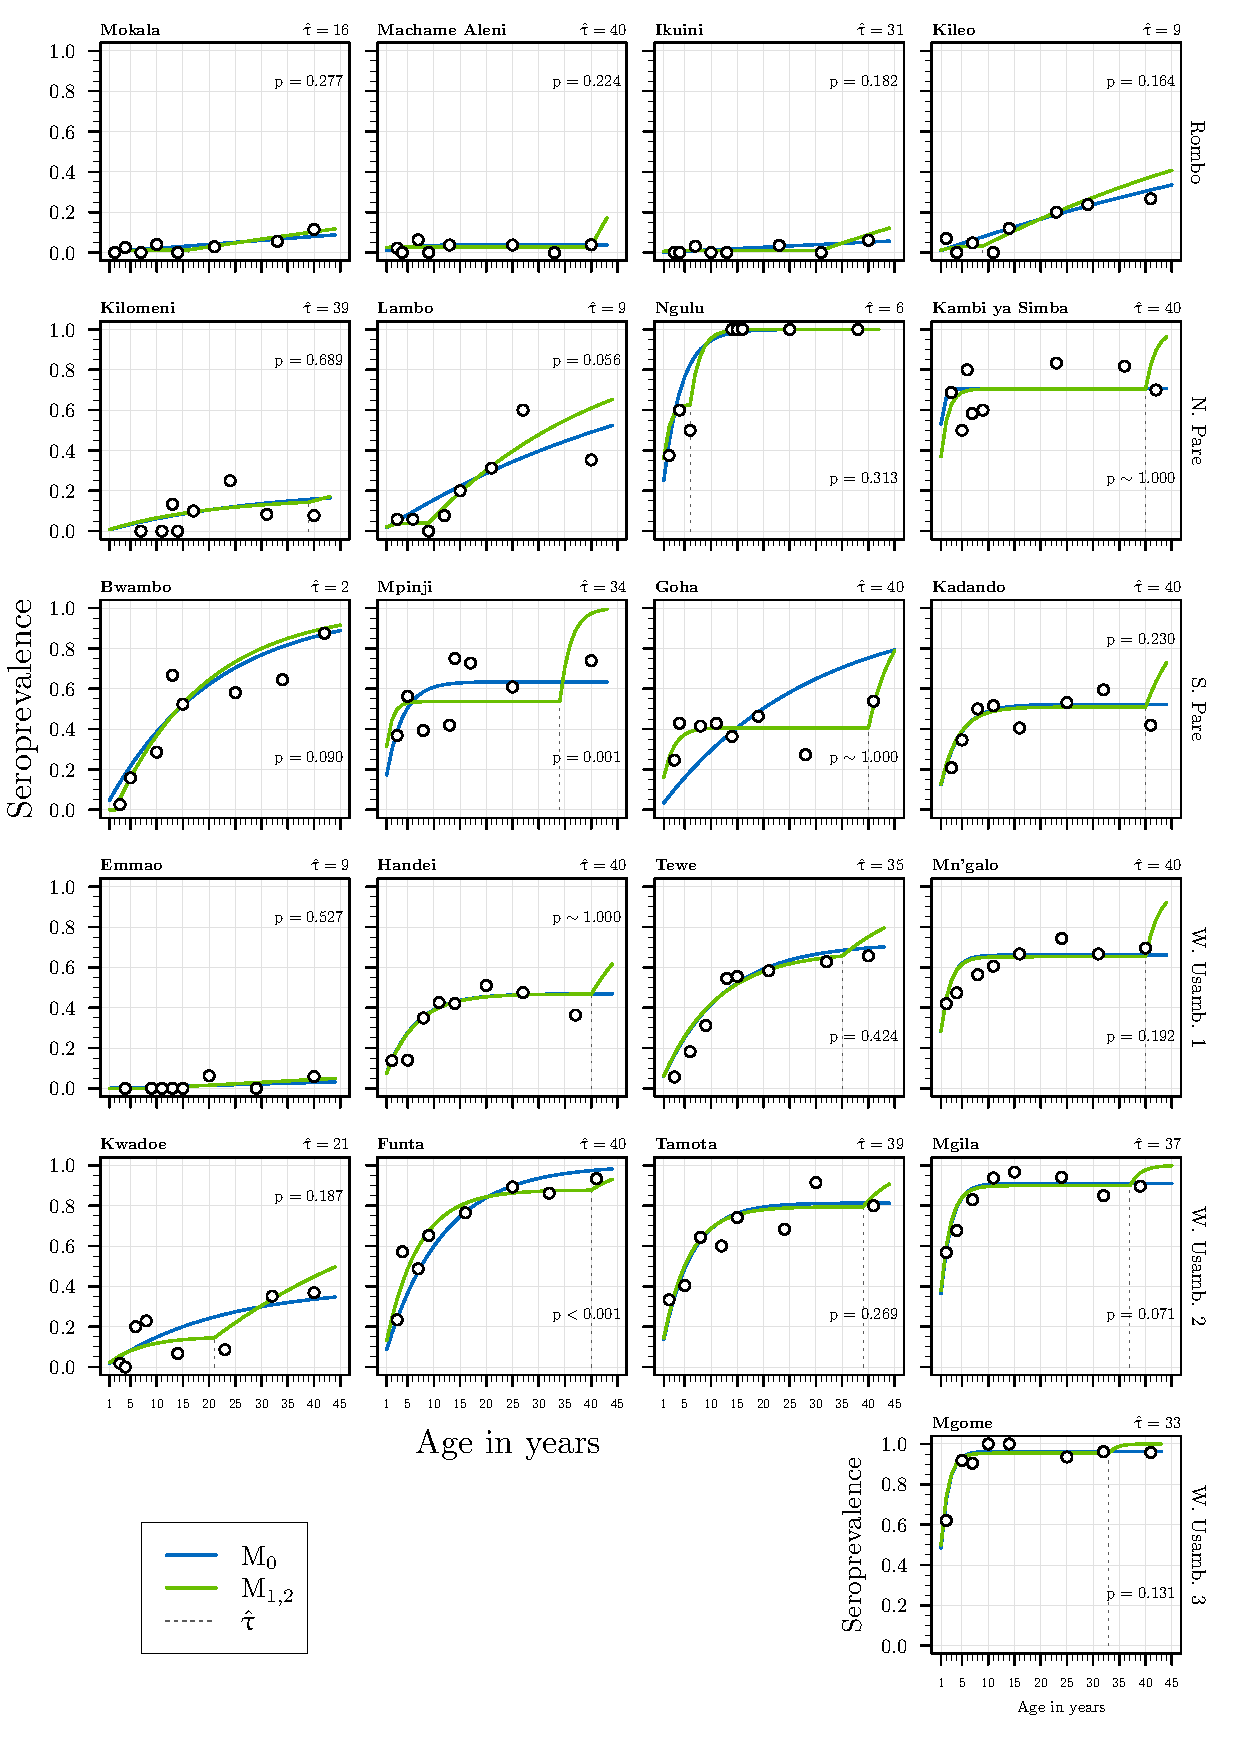
\includegraphics[width=\columnwidth]{images/Seroprevalence_M0vM12_msp2.pdf}
\end{adjustbox}
\caption[Estimated MSP2 seroprevalence for models M$_0$ and M$_{1,2}$]{Fits for the estimated MSP2 antigen seroprevalence for the 21 assessed villages, using models M$_0$ (blue lines) and M$_{1,2}$ (green lines), with the cutoff parameter of the latter signalled. Each row of graphs represents data from the transects (identified on the right hand side), where villages are ordered by decreasing altitude (and increasing malaria incidence). In the different plots, the dots represent the observed seroprevalence of distinct age groups by splitting the sampled age distribution into similar bins. P-values from the resulting likelihood ratio tests are identified.}
\label{fig:msp2.seroprevalence.M0.M12}
\end{figure}


\begin{figure}[H]
\center
\begin{adjustbox}{width=\linewidth,totalheight=\textheight-5\baselineskip}
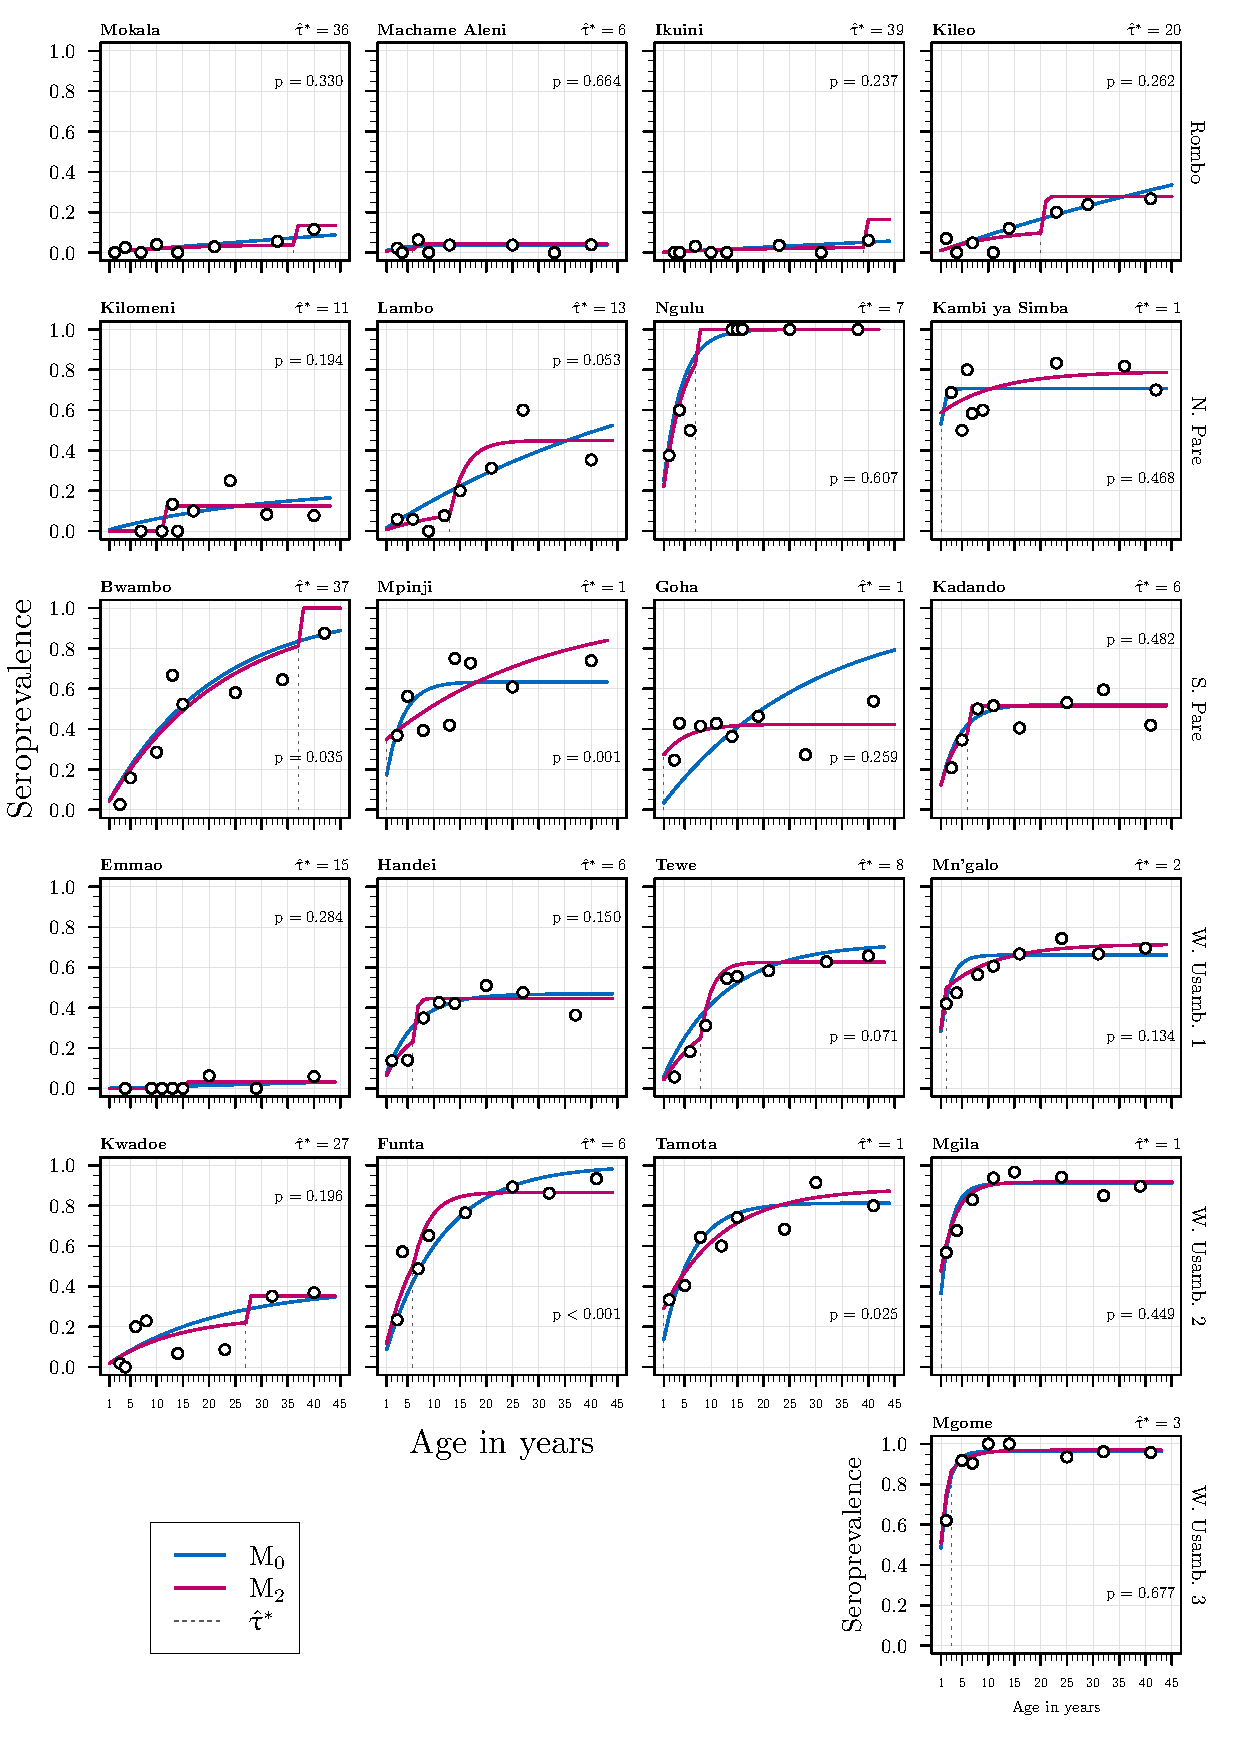
\includegraphics[width=\columnwidth]{images/Seroprevalence_M0vM2_msp2.pdf}
\end{adjustbox}
\caption[Estimated MSP2 seroprevalence for models M$_0$ and M$_2$]{Fits for the estimated MSP2 antigen seroprevalence for the 21 assessed villages, using models M$_0$ (blue lines) and M$_2$ (light red lines), with the cutoff parameter of the latter signalled, identifying the change in SCR happening in years before sampling. Each row of graphs represents data from the transects (identified on the right hand side), where villages are ordered by decreasing altitude (and increasing malaria incidence). In the different plots, the dots represent the observed seroprevalence of distinct age groups by splitting the sampled age distribution into similar bins. P-values from the resulting likelihood ratio tests are identified.}
\label{fig:msp2.seroprevalence.M0.M2}
\end{figure}

%%%%%%%%%%%%%%%%%%%%%%%%%%%%%%%%%%%%%%%%%%%%%%
% MODEL M2 ESTIMATED SEROPREVALENCE FOR AMA1 %
%%%%%%%%%%%%%%%%%%%%%%%%%%%%%%%%%%%%%%%%%%%%%%
\subsection{AMA1 estimated seroprevalence} \label{appendix:M2.seroprev.ama1}

\begin{figure}[H]
\center
\begin{adjustbox}{width=\linewidth,totalheight=\textheight-6\baselineskip}
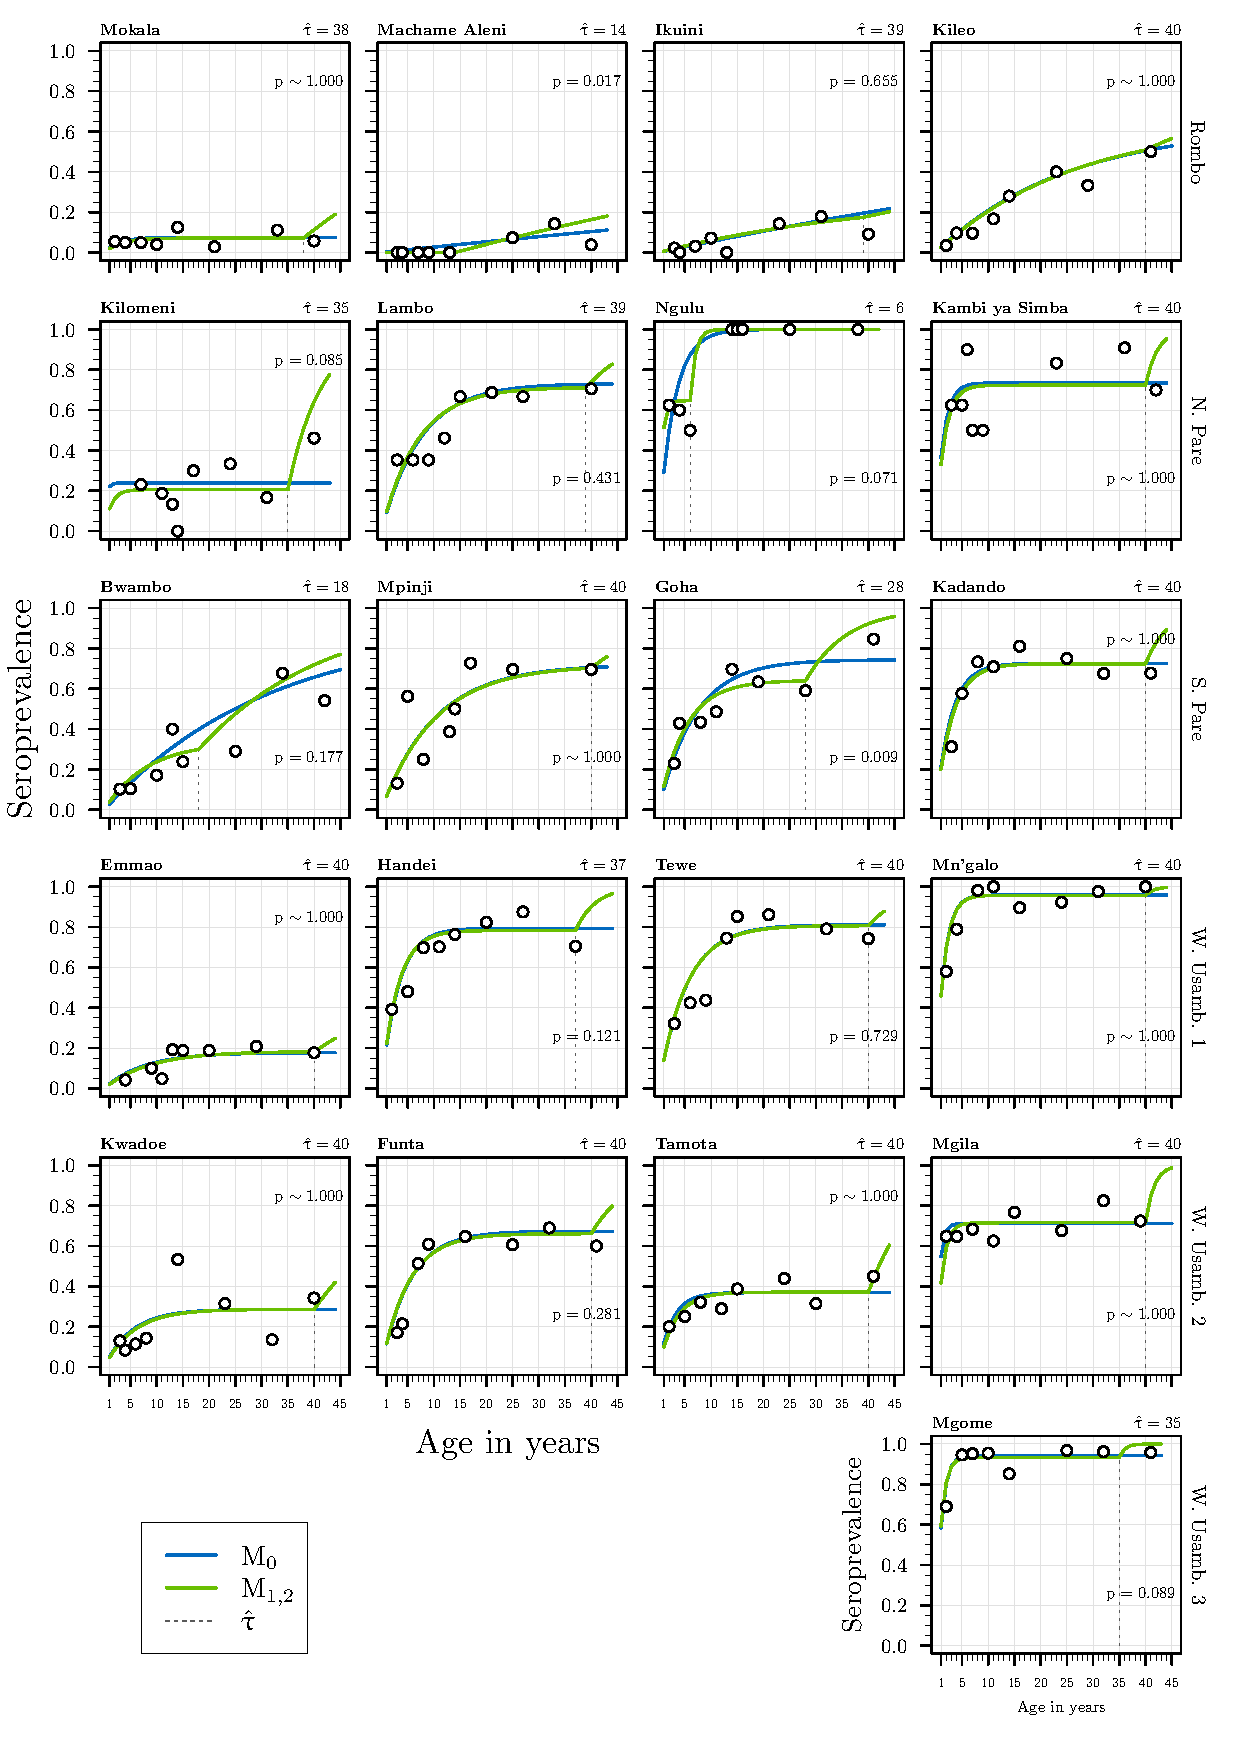
\includegraphics[width=\columnwidth]{images/Seroprevalence_M0vM12_ama1.pdf}
\end{adjustbox}
\caption[Estimated AMA1 seroprevalence for models M$_0$ and M$_{1,2}$]{Fits for the estimated AMA1 antigen seroprevalence for the 21 assessed villages, using models M$_0$ (blue lines) and M$_{1,2}$ (green lines), with the cutoff parameter of the latter signalled. Each row of graphs represents data from the transects (identified on the right hand side), where villages are ordered by decreasing altitude (and increasing malaria incidence). In the different plots, the dots represent the observed seroprevalence of distinct age groups by splitting the sampled age distribution into similar bins. P-values from the resulting likelihood ratio tests are identified.}
\label{fig:ama1.seroprevalence.M0.M12}
\end{figure}

\begin{figure}[H]
\center
\begin{adjustbox}{width=\linewidth,totalheight=\textheight-5\baselineskip}
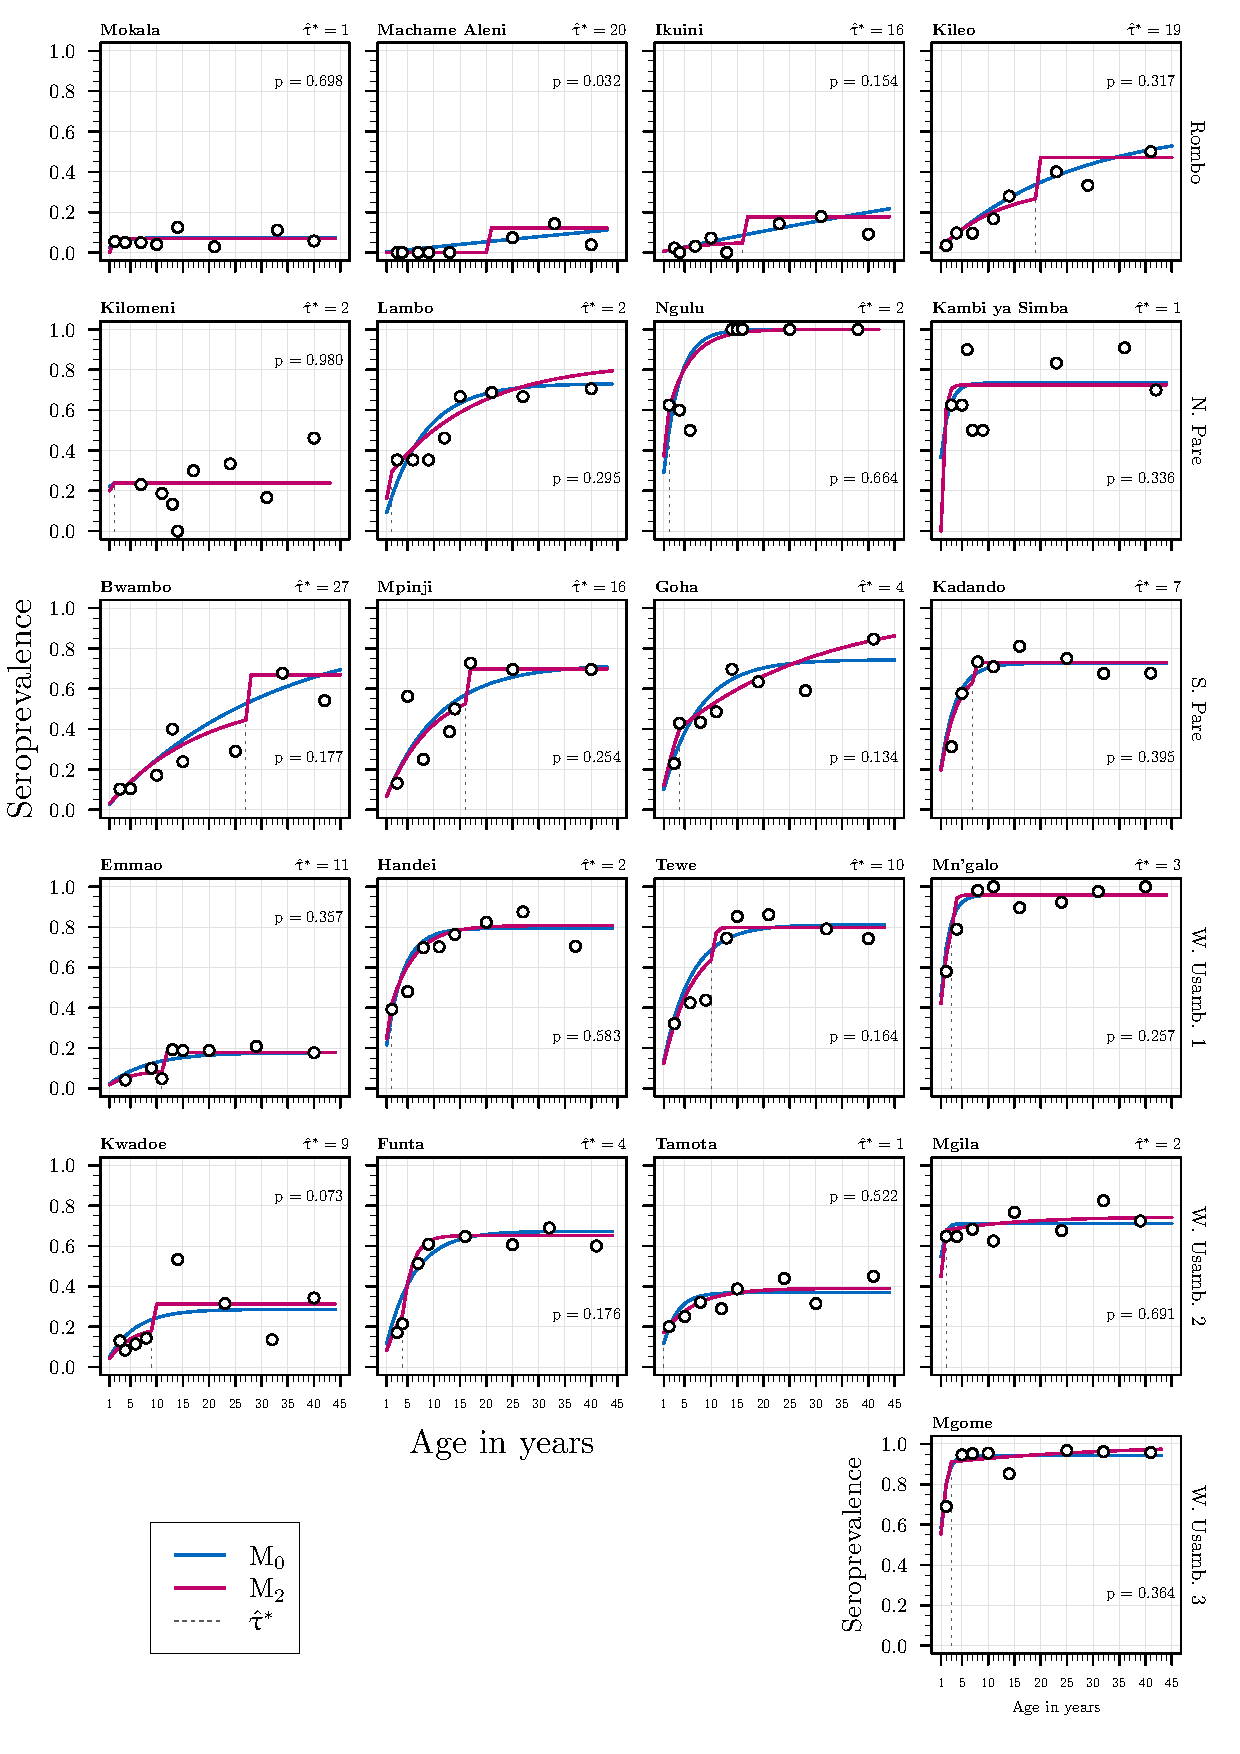
\includegraphics[width=\columnwidth]{images/Seroprevalence_M0vM2_ama1.pdf}
\end{adjustbox}
\caption[Estimated AMA1 seroprevalence for models M$_0$ and M$_2$]{Fits for the estimated AMA1 antigen seroprevalence for the 21 assessed villages, using models M$_0$ (blue lines) and M$_2$ (light red lines), with the cutoff parameter of the latter signalled, identifying the change in SCR happening in years before sampling. Each row of graphs represents data from the transects (identified on the right hand side), where villages are ordered by decreasing altitude (and increasing malaria incidence). In the different plots, the dots represent the observed seroprevalence of distinct age groups by splitting the sampled age distribution into similar bins. P-values from the resulting likelihood ratio tests are identified.}
\label{fig:ama1.seroprevalence.M0.M2}
\end{figure}



%%%%%%%%%%%%%%%%%%%%%%%%%%%%%%%%%%%%%%%%%%%%%%%%%%%%%
% R FUNCTIONS TO ESTIMATE TRANSITION RATES FROM M11 %
%%%%%%%%%%%%%%%%%%%%%%%%%%%%%%%%%%%%%%%%%%%%%%%%%%%%%

\subsection{R functions used to estimate transition rates from model M$_{1,1}$}
\label{appendix:r.function}
\definecolor{mygreen}{rgb}{0,0.6,0}
\definecolor{mygray}{rgb}{0.5,0.5,0.5}
\definecolor{mymauve}{rgb}{0.58,0,0.82}
\lstset{
        language=R,
        basicstyle=\scriptsize\ttfamily,
        commentstyle=\ttfamily\color{mygreen},
        numbers=left,
        numberstyle=\ttfamily\color{black}\footnotesize,
        stepnumber=1,
        numbersep=5pt,
        backgroundcolor=\color{white},
        showspaces=false,
        showstringspaces=false,
        showtabs=false,
        frame=single,
        tabsize=2,
        captionpos=b, % sets the caption-position to bottom
        breaklines=true, % sets automatic line breaking
        breakatwhitespace=false, % sets if automatic breaks should only happen at whitespace
        title=\lstname,
        escapeinside={},
        keywordstyle={},
        morekeywords={},
        backgroundcolor=\color{white}, % choose the background color; you must add \usepackage{color} or \usepackage{xcolor}; should come as last argument
        keepspaces=true,                 % keeps spaces in text, useful for keeping indentation of code (possibly needs columns=flexible)
        keywordstyle=\ttfamily\color{blue},       % keyword style
        morekeywords={*,...},            % if you want to add more keywords to the set
        numbersep=5pt,                   % how far the line-numbers are from the code
        rulecolor=\color{black},         % if not set, the frame-color may be changed on line-breaks within not-black text (e.g. comments (green here))
        title=\ttfamily{jtm\_functions\_M11.R}
}

\lstinputlisting[language=R]{appendices/jtm_functions_M11.R}

\end{appendices}

\pagestyle{plain}
\cleardoublepage

\end{document}